%% Use the standard UP-methodology class
%% with French language.
%%
%% You may specify the option 'twoside' or 'oneside' for
%% the document.
%%
%% See the documentation tex-upmethodology on
%% http://www.arakhne.org/tex-upmethodology/
%% for details about the macros that are provided by the class and
%% to obtain the list of the packages that are already included. 
 
\documentclass[english]{spimubphdthesis}

%%--------------------
%% The TeX code is entering with UTF8
%% character encoding (Linux and MacOS standards)
\usepackage[utf8]{inputenc}
 
%%-------------------
%% You want to use the NatBib extension
%\usepackage[authoryear]{natbib}
 
%%--------------------
%% Include the 'multibib' package to enable to
%% have different types of bibliographies in the
%% document (see at the end of this template for
%% an example with a personnal bibliography and
%% a general bibliography)
%%
%% Each bibliography defined with 'multibib'
%% adds a chapter with the corresponding
%% publications (in addition to the chapter for
%% the standard/general bibliography).
%% CAUTION:
%% There is no standard way to do include this type of
%% personnal bibliography.
%% We propose to use 'multibib' package to help you,
%% for example.
% \usepackage{multibib}
 
%% Define a "type" of bibliography, here the PERSONAL one,
%% that is supported by 'multibib'.
%\newcites{PERSO}{Liste de mes publications}
 
%% To cite one of your PERSONAL papers with the style
%% of the PERSONAL bibliography: \citePERSO{key}
%% To force to show one of your PERSONAL papers into
%% the PERSONAL bibliography, even if not cited in the
%% text: \nocitePERSO{key}
 
%% REMARK: When you are using 'multibib', you
%% must compile the PERSONAL bibliography by hand.
%% For example, the sequence of commands to run
%% when you had defined the bibliography PERSO is:
%%   $ pdflatex my_document.tex
%%   $ bibtex my_document.aux
%%   $ bibtex PERSO.aux
%%   $ pdflatex my_document.tex
%%   $ pdflatex my_document.tex
%%   $ pdflatex my_document.tex


%%--------------------
%% Add here any other packages that are needed for your document.
%\usepackage{eurosim}
%\usepackage{amsmath}
\usepackage{graphicx}
\usepackage{epsfig}
\usepackage{mathrsfs}
\usepackage{times}
\usepackage{makeidx}
\usepackage{amsmath}
\usepackage{algorithm}
\usepackage{algorithmic}
%\usepackage{subfigure}
%\usepackage{subcaption}
\usepackage{multicol}
\usepackage{array}
\usepackage{siunitx}
\usepackage{balance} % This allows for the even columns in the final page, just insert \balance in the last page, e.g., before the reference list
\usepackage{cite}
%\usepackage{setspace}
\usepackage{etoolbox}
\newtoggle{blindcopy}
%\toggletrue{blindcopy}
\usepackage{hhline}
\usepackage{booktabs}
\usepackage{rotating}
\usepackage{multirow}
\usepackage{wasysym}
\usepackage{xcolor}
\usepackage{adjustbox}
\usepackage{slashbox}
\usepackage{threeparttable}
\usepackage{blindtext}

%\usepackage{subfigure}
\usepackage[subrefformat=parens,labelformat=parens]{subcaption}

\usepackage{listings}
\lstset{
	basicstyle=\ttfamily,
	columns=fullflexible,
	breaklines=true,
	postbreak=\mbox{\textcolor{black}{$\hookrightarrow$}\space},
}

% set new command for table column width
\usepackage{array}
\newcolumntype{L}[1]{>{\raggedright\let\newline\\\arraybackslash\hspace{0pt}}m{#1}} % left aligned
\newcolumntype{C}[1]{>{\centering\let\newline\\\arraybackslash\hspace{0pt}}m{#1}} % center aligned
\newcolumntype{R}[1]{>{\raggedleft\let\newline\\\arraybackslash\hspace{0pt}}m{#1}} % right aligned

%\usepackage{etoolbox}
%\newtoggle{usingspim}
%\toggletrue{usingspim}
%\togglefalse{usingspim}


%paragraph indentation
\setlength{\parindent}{4em} 

%paragraph spacing
\setlength{\parskip}{1em}

%Line spacing
\renewcommand{\baselinestretch}{1.1}

 
%%--------------------
%% Set the title, subtitle, defense date, and
%% the registration number of the PhD thesis.
%% The optional parameter is the subtitle of the PhD thesis.
%% The first mandatory parameter is the title of the PhD thesis.
%% The second mandatory parameter is the date of the PhD defense.
%% The third mandatory parameter is the location/city of the PhD defense.
%% The forth mandatory parameter is the reference number given by
%% the University Library after the PhD defense.
%\declarethesis[]{Estimation de performance, Test et Contrôle des Systèmes d’Objets Connectés Utilisant un Réseau de Communication Non-Idéal}{3 July 2020}{Dijon}{XYZ}
\declarethesis[]{Performance Estimation, Testing, and Control of Cyber-Physical Systems Employing Non-Ideal Communications Networks}{4 Sep 2020}{Dijon}{XYZ}
%{Estimation de performance, Test et Contrôle des Systèmes d’Objets Connectés Utilisant un Réseau de Communication Non-Idéal}


 
%%--------------------
%% Set the author of the PhD thesis
\addauthor[rick.candell@gmail.com]{Richard Candell}{}


 
%%--------------------
%% Add a member of the jury
%%
%% CAUTION 1: If a Jury member is not present during the defense,
%%            she/he must be in the list of the Jury members.
%%            Only the reviewers and the members who are present during the defense must
%%            appear in the Jyry member list. 
%% CAUTION 2: After your defense, you must assign the role "Pr\'esident" to
%%            the Jury member who have been the President of the Jury.
%% CAUTION 3: The recommended order for the Jury members is:
%%            President, Reviewer(s), Examiner(s), Director(s),
%%            Other supervisor(s), Invited person(s).
%% \addjury{Firstname}{Lastname}{Role in the jury}{Position}
%\addjury{Alain}{BONNIN}		{Pr\'esident}			{Universit\'e de Bourgogne \\ Commentaire secondaire}
\addjury{Sebti}{FOUFOU}		{Directeur de thèse}	{Professeur à l'Universit\'e de Bourgogne}
\addjury{Khalil}{DRIRA}	    {Rapporteur}			{Professeur à l'Universit\'e de Toulouse}
\addjury{Abbes}{AMIRA}	    {Rapporteur}			{Professeur à De Montfort University}
\addjury{Salima}{BENBERNOU}	{Examinateur}			{Professeur à l'Universit\'e Paris Descartes}
\addjury{Nejib}{MOALLA}		{Examinateur}			{Professeur à l'University Lumi\'ere Lyon 2}

 
%%--------------------
%% Change style of the table of the jury
%% \Set{jurystyle}{put macros for the style}
%\Set{jurystyle}{\small}
 
%%--------------------
%% Set the English abstract
\thesisabstract[english]{Wireless technology is a key enabler of the promises of Industry 4.0 (Smart Manufacturing). As such, wireless technology will be adopted as a principal mode of communication within the factory beginning with the factory enterprise and eventually being adopted for use within the factory workcell.  Factory workcell communication has particular requirements on latency, reliability, scale, and security that must first be met by the wireless communication technology used.  Wireless is considered a non-ideal form of communication in that when compared to its wired counterparts, it is considered less reliable (lossy) and less secure.  These possible impairments lead to delay and loss of data in industrial automation systems where determinism, security, and safety are considered paramount.  This thesis investigates the wireless requirements of the factory workcell and applicability of existing wireless technology, presents a modeling approach to discovery of architecture and data flows using SysML, provides a method for the use of graph databases to the organization and analysis of performance data collected from a testbed environment, and, finally, provides an approach to using machine learning in the evaluation of cyberphysical system performance.}

 
%%--------------------
%% Set the English keywords. They only appear if
%% there is an English abstract
\thesiskeywords[english]{industrial wireless, smart manufacturing, systems modeling, machine learning, graph database, industrial wireless testbed}


%%--------------------
%% Set the French abstract
\thesisabstract[french]{Lorem ipsum dolor sit amet, saepe quodsi dolores an usu. An sed fugit dissentiunt, ex tota soleat duo. Omnes deserunt adversarium qui ad, periculis pertinacia has id. Ea tibique antiopam eos. Usu illud cetero voluptatum ne, ea odio soluta labores sit.	Pri modus eruditi definiebas an. Dicat latine inermis no quo, eos tollit delicata interesset cu. Placerat vituperatoribus pro ne, cu verear tritani deterruisset usu. Quaeque recusabo maluisset te pri, mutat maiorum accusamus at his.	Pro ad nihil deleniti senserit, mundi feugiat indoctum an sea. In consulatu efficiendi qui, eu duo dicta deserunt definitiones, te atqui sapientem adolescens sit. Id pro consulatu splendide evertitur, vis eu perpetua molestiae, an melius virtute efficiantur vis. Animal aeterno mei ei.	}


%%--------------------
%% Set the French keywords. They only appear if
%% there is an French abstract
\thesiskeywords[french]{communications sans fil industriel, fabrication intelligente, apprentissage automatique, modelisation systéme, base de données graphe, banc d'essai sans fil industriel}

 
%%--------------------
%% Change the layout and the style of the text of the "primary" abstract.
%% If your document is written in French, the primary abstract is in French,
%% otherwise it is in English.
%\Set{primaryabstractstyle}{\tiny}
 
%%--------------------
%% Change the layout and the style of the text of the "secondary" abstract.
%% If your document is written in French, the secondary abstract is in English,
%% otherwise it is in French.
%\Set{secondaryabstractstyle}{\tiny}
 
%%--------------------
%% Change the layout and the style of the text of the "primary" keywords.
%% If your document is written in French, the primary keywords are in French,
%% otherwise they are in English.
%\Set{primarykeywordstyle}{\tiny}
 
%%--------------------
%% Change the layout and the style of the text of the "secondary" keywords.
%% If your document is written in French, the secondary keywords are in English,
%% otherwise they are in French.
%\Set{secondarykeywordstyle}{\tiny}
 
%%--------------------
%% Change the speciality of the PhD thesis
\Set{speciality}{Informatique}
 
%%--------------------
%% Change the institution
\Set{universityname}{Universit\'e de Bourgogne}
 

%%--------------------
%% Clear the list of the laboratories
\resetlaboratories

%%--------------------
%% Add the laboratory where the thesis was made
%\addlaboratory{Laboratoire Waynes Industry}
\addlaboratory{Laboratoire \'Electronique, Informatique et Image}


%%--------------------
%% Clear the list of the partner/sponsor logos
%\resetpartners

%%--------------------
%% Add the logos of the partners or the sponsors on the front page
%%
%% CAUTION 1: At least, the logo of the University should appear (UB)
%%
%\addpartner[image options]{image name}

%\addpartner{ub}

%%--------------------
%% Change the header and the foot of the pages.
%% You must include the package "fancyhdr" to
%% have access to these macros.
%% Left header
%\lhead{}
%% Center header
%\chead{}
%% Right header
%\rhead{}
%% Left footer
%\lfoot{}
%% Center footer
%\cfoot{}
%% Right footer
%\rfoot{}
 
%%--------------------
% Declare several theorems
%\declareupmtheorem{mytheorem}{My Theorem}{List of my Theorems}

%%--------------------
%% Change the message on the backcover.
%\Set{backcovermessage}{%
%	Some text
%}

\begin{document}
 
%%--------------------
%% The following line does nothing until
%% the class option 'nofrontmatter' is given.
\frontmatter

%%--------------------
%% The following line permits to add a chapter for "acknowledgements"
%% at the beginning of the document. This chapter has not a chapter
%% number (using the "star-ed" version of \chapter) to prevent it to
%% be in the table of contents
\chapter*{Dedication}
The author would like express his gratitude to his beautiful daughter, Erin, for all of her
generous support, kindness, and care, and her countless hours as a child accompanying me in my laboratory. I hope that she
remembers fondly those weekends listening to her Avengers movies while I ran factory simulators and troubleshooted robots.


%%--------------------
%% The following line permits to add a chapter for "acknowledgements"
%% at the beginning of the document. This chapter has not a chapter
%% number (using the "star-ed" version of \chapter) to prevent it to
%% be in the table of contents
\chapter*{Acknowledgments}

My deepest gratitude goes to my Lord, God, for all of His support, guidance, training, and wisdom.  Without the endowment of my abilities by Him, this work would have been made impossible.  I have been blessed with intelligence and creativity sufficient to perceive a vision, communicate that vision, and then direct a team more capable than myself to implement that vision.  I would like to extend my deepest thanks to my research team.  Without their help during trying times, this thesis would have been possible. I would like to acknowledge my advisor, Professor Foufou, whose steadfast encouragement to persevere has not gone unnoticed. 

	
%%--------------------
%% Include a general table of contents
\setcounter{tocdepth}{2}
\tableofcontents

%%--------------------
%% The content of the PhD thesis
\mainmatter

\fontencoding{T1}
\fontfamily{times}
\fontseries{m}
\fontshape{it}
\fontsize{12}{15}
\selectfont
 
\part{Context and Problem Statement}\label{part:context}
\chapter{Introduction}\label{chapter:intro}

\chapterintro*
Cyber-physical systems (CPS) are defined as a holistic integration of computing, networking, and physical processes.  Implicit within these systems are feedback connections in which the computing and networking devices affect the physical systems directly.  Traditionally, industrial computation was performed using dedicated electronics with analog process variables and control signals being communicated over twisted-pair wires.  As automation capabilities evolved, serial communications architectures such as the common field-bus were adopted.  With the advent of the Internet and Cloud Computing, Internet Protocol (IP) was adopted for more advanced data collection and control applications.  In such applications, reliability and latency requirements were not overly difficult to achieve given the existing technologies; however applications requiring tight feedback timing and reliability were not addressed as the protocols primarily targeted slower flow-based processes and building automation.  Discrete manufacturing requirements remained largely unaddressed.  To answer the call of discrete manufacturing requirements, routable industrial IP protocols such as Common Internet Protocol (CIP), SERCOS III, and Profinet by Siemens were developed to guarantee latency, reliability, and interoperability between systems.  However, given that these protocols are often IP-routable and share a common communication medium, these types of systems are limited in their ability to meet the performance demands of the physical systems or guarantee security.   These wired protocols can lack flexibility and mobility demanded by modern industrial applications.

Communication strategies that jointly address reliability, timing, scale, and power are needed to meet the needs of future industrial control systems.  Proponents of advanced manufacturing systems such as those defined by Industry 4.0 and the Industrial Internet Consortium state that existing protocols are not capable of meeting all the demands of industry.  The future factory will require untethered situationally-aware communications, heavy reliance on automation to include robotics, and an increased cognitive cyber-security posture.  It is not certain if feedback control of robot motion is necessary; however, future communication systems must address strict latency and data reliability requirements for discrete sensors, actuators, and robot end-effectors while maintaining security.  With the adoption of wireless communications in the factory, existing protocols such as IEEE 802.11 and IEEE 802.15.4 are not be capable of meeting reliability demands, round-trip latencies under 10ms, or scalability to dozens of devices within individual workcells and hundreds or thousands of devices within an entire factory system.    

Wireless communications is inherently more prone to latency and delay than wired counterparts.  In addition, wireless communication implies the utilization of the electromagnetic spectrum which is a publicly accessible medium with constrained capacity and more prone to cyber-attack.  While transmitted data can by digitally protected through authentication and encryption, wireless devices are prone to interference and jamming by both rogue and friendly emitters, exacerbating the reliability and latency concern impacting factory performance without compromising data security.  Wireless communication in factories is often constrained by battery life and most certainly constrained by the availability of the electromagnetic spectrum.   As the reliance on wireless devices within the factory continues, steps toward developing a more robust wireless factory communications network must be developed. These steps include:

\begin{itemize}
	\item The automation system must become state aware and adaptive to knowledge of the trends in electromagnetic spectrum occupancy and acute events; 
	\item Intelligence of the automation system must move closer to the physical system.  This means moving the intelligence for control to the actuator; and  
	\item Performance test methods must be developed and incorporated into the industrial fringe devices.  The test methods must be dependable and at the same time easy to use by factory personal not trained in the technicalities of wireless communication. 
	\item Existing Wireless communications protocols must be analyzed and adapted, and new protocols must be developed to balance reliability, latency, and scalability. 
	\item Security of the network must be maintained and must include availability as a paramount characteristic.
\end{itemize}

The proposed thesis presents the development of test approaches for measuring the performance of industrial wireless networks deployed within smart manufacturing workcells.  Thus the primary goal of this thesis is the discovery of methods and approaches to the evaluation of industrial uses cases performance for those use case in which wireless communication technology is used as the principal mode of communications.  The primary motivation of the research has been to discover practical test and evaluation methods for assessing performance of an industrial workcell thereby improving security, safety, and reliability.   Findings and results of the thesis work are included within this thesis and published as journal articles and conference proceedings.  These references are noted through the text and bibliography.  

\section{Industrial Revolutions}
Major advances in manufacturing of goods for the betterment of humanity have occurred many times in the last two hundred and fifty years in the history of humanity.  These advancements occurred of science and technology occurred as revolutionary events at different times.  The first revolution occurred at the edge of the eightieth century primarily in England but also in France, Germany, and the United States with the applicant of automatic mechanization of large machines using coal powered steam engines.  These machines were mainly used for the processing of cotton, wool, and silks in the production of textiles for export throughout the world.  Advancements during this period included uses of coal to produce steam power, the production of iron, steel, and other rudimentary alloys, and, very importantly, the engineering advancements of tool making.  The advancements of the first industrial revolution paved the way for the centralization and mass production of goods.
%CITATION SOURCES *** {https://en.wikipedia.org/wiki/Technological_revolution#Potential_future_technological_revolutions}

The next century was marked by the development of scientific and engineering advancements in chemistry, physics, and engineering. Experimentation with electricity and the production thereof led to the eventual explosion of industrial machinery, tooling, electrification, chemical manufacture, petroleum refinement, rail and marine transportation, the automobile, agriculture, and telecommunications by wire over long distances.  This period of discovery culminated with rapid expansion of industrialization through the world, especially in North America and Japan up until the beginning of World War I.
%CITATION SOURCES *** https://en.wikipedia.org/wiki/Second_Industrial_Revolution#Machine_tools

\begin{figure}[!tbp]
	\begin{center}
		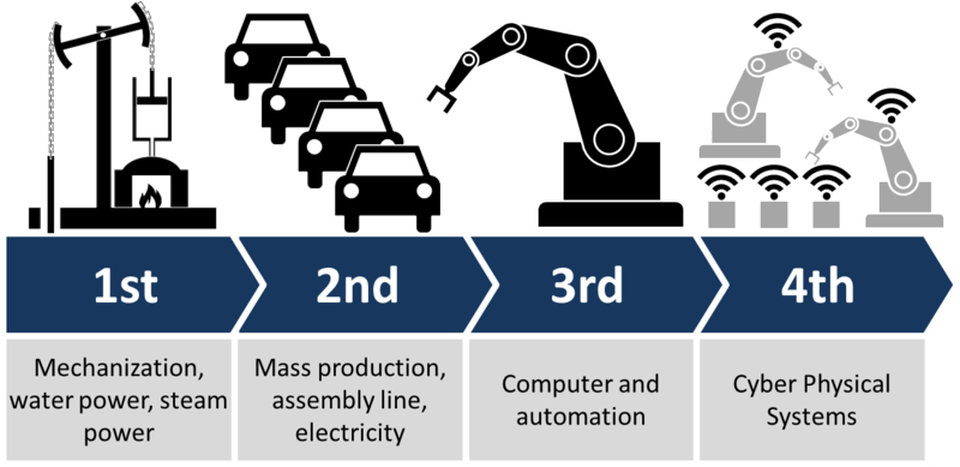
\includegraphics[width=0.75\textwidth]{chapter-intro/images/forbes_2016_03_Industry_4.0}
		\label{fig:intro:forbes-i40-evolution}
		\caption{Industry 4.0: Wireless is a key enabler in the 4th industrial revolution.}
	\end{center}
\end{figure}

The third industrial revolution began in the tears immediately following the second world war with the rapid advancement of pure and applied sciences.  These advancements were driven primarily by the cold war and the space race between the United States and the USSR.  This period of advancement was marked by many discoveries and scientific applications such as the development of telecommunications theories (Claude Shannon), advancement of radio and wired communications, the discovery of the transistor, and the rapid expansion of computers and information technology in business and defense.  Also during these years, arrived the application of computing within manufacturing and process control settings. Computers slowly began to replace the basic relay circuit in control systems.  By utilizing the programmable logic controller (PLC), manufacturers gained the ability to develop control their processes more easily and develop control strategies that were once more difficult to implement in the past with dedicated, specialized equipment.  PLCs offered both the ability to more easily adapt processes to information gathered directly from the factory operation as well as slowly collect and store information electronically.  However, electronic storage of this information was still both difficult and expensive as telecommunications technology was yet relatively slow and storage expensive.  Over the years following through the 1980's until today, computers have followed closely Moore's "Law" which states according to the the perception of Intel Corporation founder, Gordon E. Moore, that the number of transistors on a microchip doubles every two years.  This paradigm of exponential growth in digital computing technology in terms of computing speed, storage, and efficiency has created a world in which computers and computing devices have become ubiquitous, surrounding practically every aspect of human endeavors and leading to the latest installment of industrial advancement, the 4\textsuperscript{th} Industrial Revolution, also known as the \textit{Information Revolution} which is currently ongoing. 

The Information Revolution is defined by a culture that is highly interconnected and data-dependent.  Clearly, the modern world is dominated by the Internet, high-performance computers, and personal mobile communications devices such as cell phones developed over the last several decades. Within the hands of each individual, one may find a smartphone capable of performing computing and communications tasks not even imaginable fifty years ago.  Indeed, within each of these devices resides a powerful microprocessor capable of clocking speeds in the gigahertz, offline storage spanning gigabytes, at-least one high-resolution camera, and communication components enabling high-speed connectivity capability.  These personal devices are smart and easily re-programmable by downloading of new applications, i.e., \textit{apps} enabling users to produce and consume information rapidly.  Users enjoy the ability to speak at any moment, send brief messages using apps such as WhatsApp\texttrademark, download videos, play games, store documents, music, photographs, and videos within "the cloud."  Within office and business enterprises, a personal computer is within reach of every employee and is the tool used for information production.  The data produced is stored within the cloud and usually produced and maintained locally, although the services of data production are quickly shifting to the cloud as well depending on the needs the end user.

These capabilities have also been permeating industrial environments, although at a slower rate, given the inherent conservatism of industrial establishments.  Industrial environments include aerospace and automotive manufacturing, electrical power production, food processing, petroleum and chemical production.  That is not to say that industrial establishments are not open to technological change, but that established production system can be difficult or risky to modify once they are operational.  While industrial operations have distinctly different requirements than office businesses; analogues may be made between the computing constructs found within the personal/business computing domains and those constructs founds within the industrial computing domains.  For example, within a factory production enterprise, the Internet itself exists as an outside entity providing global connectivity, hosting, storage, computing resource, and analysis tools.  These services are often replicated within the business enterprise of the factory operation and extended into the factory environment to some degree from the factory management system to the factory floor.  

In addition, with the explosiveness of ubiquitous, low-cost computing devices, the modern factory operation is changing to include more intelligence and adaptability at the factory edge.  This change includes discrete devices such as sensors and actuators, collaborative robots, autonomous gantry systems, intelligent vehicular systems, tracking and inventory systems, and the like.  These systems coupled with the plethora of computing resources have the potential to create an enormous amount of information as well as the opportunities for greater control over the factory enterprise.  It is just a matter of tapping the information within the factory and bringing that information to a useful purpose.  Where the third industrial revolution brought computing and automation to the factory, the fourth industrial revolution will improve upon the automation found within the factory by adding intelligence, autonomy, and machine learning powered by data. This data-centricty defines Industry 4.0.  

\section{Industry 4.0 and Smart Manufacturing}

Industry 4.0 was \textit{officially} launched by President Barack Obama of the United States and Chancellor Angela Merkel of Germany at the Hannover Messe industry show on April 24, 2016 \cite{HannoverMesse2016:Report, HannoverMesse2016:MachineDesign}.  Smart manufacturing is a term used to described the ongoing efforts within academia, government, and private industry to improve upon existing and future factory operations by incorporating the latest advances and design principals in computing, storage, and communication such as interoperability, virtualization, decentralization, distributed control, real-time processing and communication, service oriented architecture, easy use and maintenance, cost savings, and modularity of design.  With Industry 4.0, the industrial internet of things (IIoT) and industrial cyber-physical systems are expected to make large sweeping changes in efficiency, reliability, and capability of the future factory~\cite{Raptis2019}.	

\begin{figure}[!tbp]
	\begin{center}
		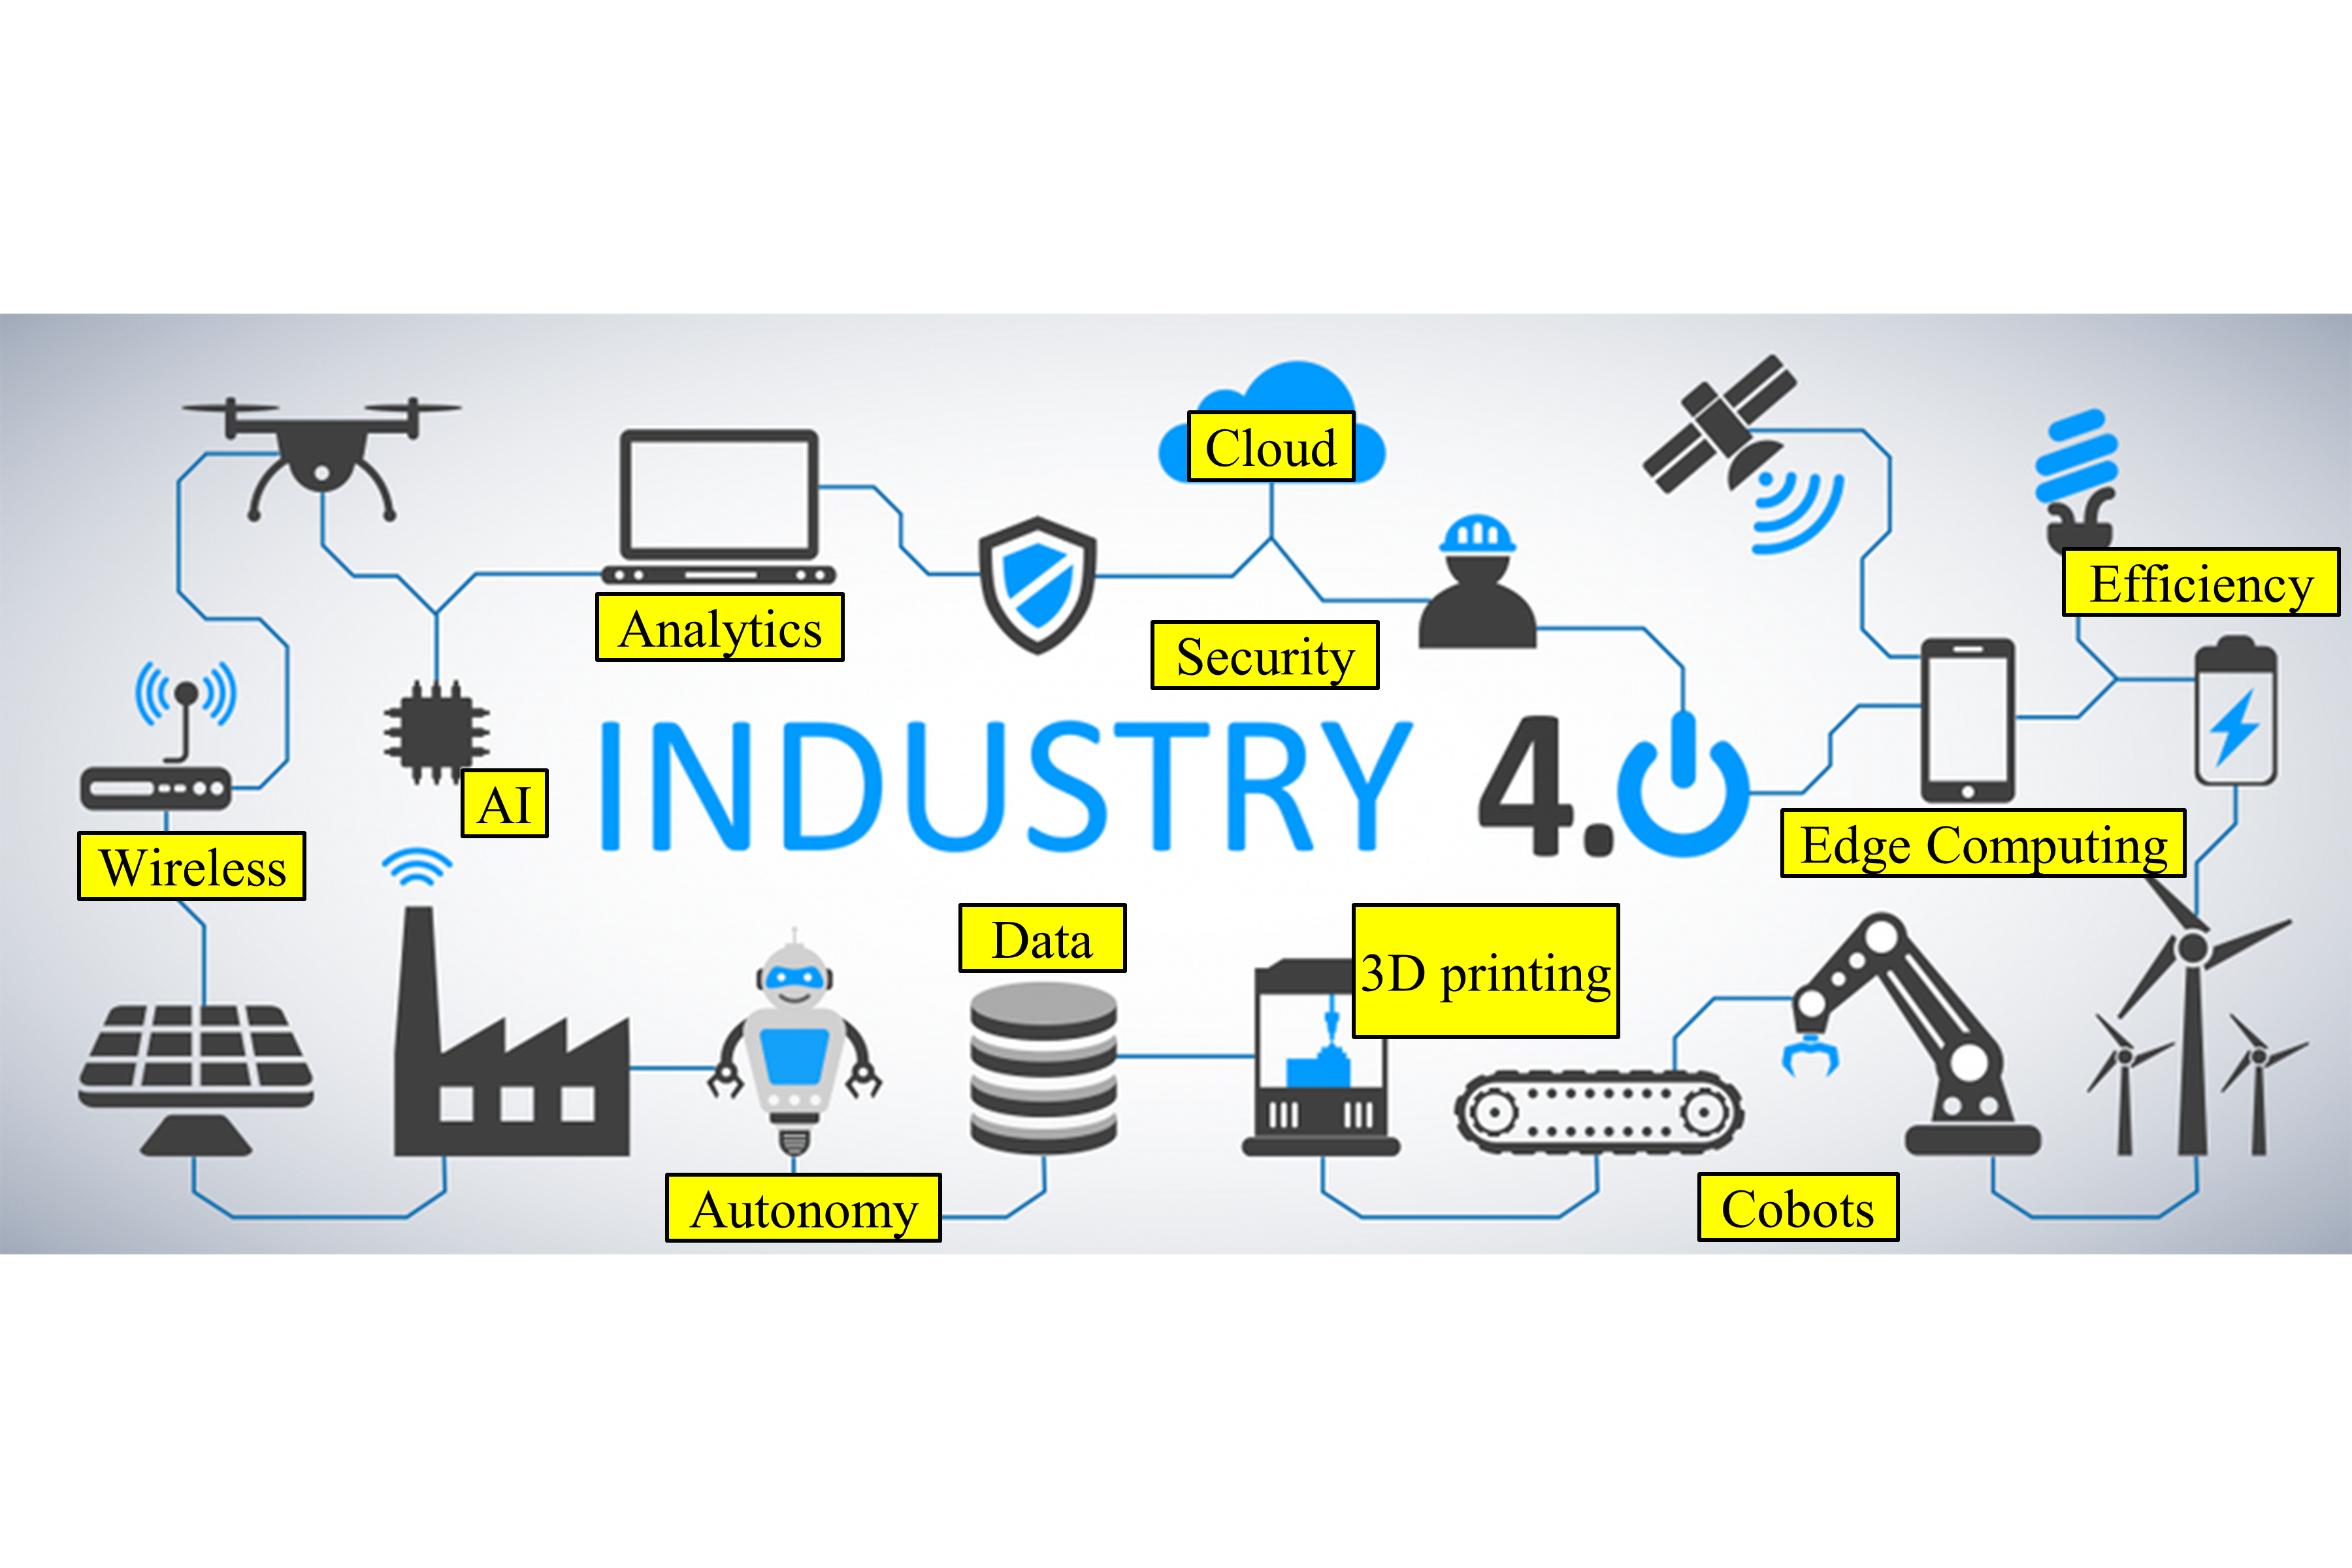
\includegraphics[width=\textwidth]{chapter-intro/images/intro/forbes-i40-candell.png}
		\label{fig:intro:forbes-i40}
		\caption{Industry 4.0: Incorporating the benefits of machine learning, massive data, mobility, and autonomy within the modern factory.}
	\end{center}
\end{figure}
%\begin{verbatim}https://www.forbes.com/sites/bernardmarr/2018/09/02/what-is-industry-4-0-heres-a-super-easy-explanation-for-anyone/#6dee527a9788\end{verbatim}

Propelled by economic pressure toward greater efficiency, factory agility, and product customization, future factories will have the technological ability to adapt quickly to customer demands, modify manufacturing processes automatically based on quality feedback, and fabricate products with a reduced environmental impact.  Technological application and advances required for smart manufacturing to be truly successful include collaborative and mobile robotics, distributed machine autonomy based on artificial intelligence, and a high degree of interconnectivity of among the automation resources.  Some of the important technologies and capabilities within a smart factory are listed below.  This is certainly not an exhaustive list of what is required to achieve the goals of Industry 4.0, but it highlights some of the fundamentals that are pertinent to this thesis.

\begin{description}
	
	\item[Data] Quantities, signals, states, and situational awareness are essential to the goals of smart manufacturing. This knowledge will be centric to the ongoings of the future factory.  Data will be produced rapidly, transmitted, accumulated in large quantities, analyzed, and acted upon continuously; and the behavior of the smart factory will rely heavily on this data to operate. 
	 
	\item[The Cloud] These are the resources required for storage, processing, analysis, and presentation of data produced by the factory enterprise.  The resources of "The cloud" will include elements associated with the infrastructure and services offered.  These types of services would be augmented to meet the needs of the factory enterprise.
	
	\item[Edge Computing]  While much data will be stored within cloud resources, other forms of data will be migrated toward the "edge" on the floor of the factory.  Edge computing will increase efficiency making data more rapidly accessible for automation and control within the workcell.  Moving data between automation actors within the factory quickly will be essential.  Identifying the kinds of data and communications needs is equally important.
	
	\item[Robots] The smart factory will be replete with robots of all kinds including stationary and mobile arms, cranes, lifts, etc.  The robots will be mostly collaborative in that they will coexist with other robots as well as humans as they perform their own tasks or cooperate to complete them together.  Robots will have the ability to roam between work-cells within a factory, learn its role quickly, become aware of edge devices, and communicate with other actors within the workcell to accomplish its goals.  Current manufacturing architectures use wired connectivity through field bus and industrialized Ethernet for sensing and real-time control of robotics resources. By mobilizing robot resources, cables will be eliminated; therefore, reliable, high-performance wireless communication becomes essential.
	
	\item[Artifical Intelligence (AI)] Computing resources within the factory will be supplied with some form of intelligence.  The level of intelligence will depend on the applications required and the level of advancement of machine learning in general.  Much of the intelligence will be centralized in the beginning, but as the capabilities of edge devices evolve and improve, AI will migrate more towards the edge including mobile actors such as robots.   And since mobility is also essential to the goals of smart manufacturing, wireless performance will be important to enabling rapid an reliable communication between intelligence centers and mobile actors such as robots and other untethered machines.
	
	\item[Wireless Communication] A central concept to all of the previous content is the movement of data between autonomous and mobile actors within the smart factory environment.  Wireless communication is key to achieving this vision as it pertains to the transfer of information between two or more points without cables "over the air" typically using the propagation of modulated electromagnetic waves~\cite{proakis1995digital}.


\end{description}



\section{The Importance of Wireless in Smart Manufacturing}
The concept of Industry 4.0 is centered around the smart factory in which autonomous actors permeate the factory.  Wireless technology is an essential requirement for all interconnected things that are wireless. Cyber-physical systems (CPS), i.e., systems in which the networking, computation, and the physical world are tightly integrated will dominate the factory.  Whereas the factory of the past was predicated on centralized design based on limited data and knowledge of the past, present, and future states of the business enterprise, decision making within the smart factory will be highly decentralized.  Information will likely be stored in the cloud; however, the actors making decisions will be located in throughout the factory itself at the edge.  Wireless technology will be used fore two main categories within the smart manufacturing enterprise and are described as follows:

\begin{description}
	
	\item[Cable Elimination] Substitution with a wireless technology where once a wire existed in an existing industrial system.  This often occurs when the cost of installing a cable is either infeasible or prohibitively expensive but the cost of not replacing the wire would cost more.  Cable substitution with wireless could be envisioned where once a cabinet existed as a nexus point for input-output (I/O) end-points.  If a legacy product fails thus rendering the nexus in-operational, wireless could be used to replace the connections between a computing device and the various I/O endpoints.  This scenario is often cited in industry as a high-likelihood scenario for both sensing applications and sensing with control applications where the I/O end-points are stationary.  Wireless will be used to circumvent future failure or will be used as a rapid replacement measure for a failed system.
	
	\item[Mobility Enabling] Support of one or more untethered actors such as a robotic arm or heavy lift machine to assist in the movement of materials or the tending of other processes.  In these applications, the untethered actors require, at a minimum, instructions to perform their tasks.  More than likely, the mobile actor will need to remain aware of itself and its surroundings, communicate to a supervisor or other mobile actors.  Interconnection with the factory safety systems will likely be a necessity.
	
\end{description}


\section{Challenges in Industrial Wireless Networks}
Since the development of wireless sensor networks (WSN) beginning in the early 2000's much excitement has been generated by its promises~\cite{OnWorld2014}.   Development of IEEE 802.15.4 brought about such standards as WirelessHART~\cite{Song2008}, ISA100.11a~\cite{ISA100.11a}, and Zigbee as low-power mesh networking options for industry.  Other similar wireless networking technologies include LoRAWAN, Sigfox, 6TiSCH, and Wi-Fi to name a few.  These WSNs technologies were all designed primarily with the main goal of collecting information or transmitting large amounts of data rapidly in the special case of WiFi.  Industrial WSN technologies were not really intended to command or control devices, although they have been at times adapted to do so.  For example, WirelessHART and ISA100.11a have the primitives (i.e., the "hooks" to do so) and some valve control and other applications have been realized using these protocols. These types of WSN technologies were designed to support sensing with some supervisory or human-in-the-loop control with command decisions rarely occurring and without demanding reliability or latency requirements placed on the communication system.  Indeed, WSN's typically operate with 75\% link-to-link packer success rates at the physical layer.  With the advent of 5G communications, which in this context includes both cellular and wireless local area networks (WLAN) such as Wi-Fi (e.g., IEEE 802.11ax), much work has been done to characterize the wireless requirements landscape for industry as summarized in~\cite{Montgomery2019}.  The requirements landscape for industrial wireless can be organized into to main categories: 1) sensing and data gathering, and 2) control.  For the first category, many technologies already exist to support these applications, and rarely is reliability or latency a major concern for these applications.  The second category, control has garnered interest within the academic and industrial communities because of the promises of eliminating cables and enabling mobility, and hence, autonomy.  

However, the adoption of wireless for control applications has been rare to date~\cite{Martinez2019}.  The primary reasons for its evident failure is most likely reluctance on the part of control designers to use a mode of communication that on the surface appears brittle and unreliable regardless of the truthfulness behind these assumptions.  Wireless technology in general has the following perceived shortcomings that need to be addressed by the research and development community before its widespread adoption comes to fruition.  These shortcomings include the following:

\begin{description}	
	
	\item[Choices, Obsolescence, Interoperability] Many wireless alternatives exist, and the market is ever changing.  The number of choices can be confusing for factory operators trying to implement a solution that will last 10 years or more.  In comparison, wired networks are typically built on the same Ethernet or field-bus backbones that have existed for decades. When factory control engineers select networking equipment for a factory installation, they intend for those devices to last for at least ten years or more.  With a plethora of selections in the wireless market, the marketing hype surrounding those devices, and the rapidity by which technology changes, the reluctance to adopt wireless becomes clear.  
	
	\item[Link Performance] Information flow between actors within a factory operation.  Since wireless communication is by definition communication without wires across a shared physical medium, it is perceived (correctly) that wireless is not reliable.  This perception of a difference in reliability fuels the reluctance of wireless adoption within factories although the strong desire exists to do so.
	
	\item[Security] Factory operators want their networks to have the same level of security as their wired networks.  The very nature of wireless is open in terms of access to the physical communication media.  Essentially, this leaves wireless open for eavesdropping attacks assuming that the underlying encryption can be hacked.  If strong encryption is used, the wireless network can still be compromised by jamming or interference.  Security of the wireless network includes immunity from interference, fitness of data, and privacy.  Indeed, the concept of security can be extended to include all aspects of reliability, data integrity, privacy, safety, and stability of the factory operation touched by the wireless network.	
	
\end{description}

The use of wires precludes mobility and makes deployment of edge devices more expensive as each devices requires power, wires, and conduit for communication. By adopting wireless for both sensing and control of machines within the workcell, a lower-cost, untethered operation becomes achievable. Once wireless is adopted as the primary mode of communication, questions arise as to the required latency, reliability, scale, and security of the wireless network especially when the network is used for the control of machines and the assurance of safety. 

In a factory operation where wireless is used as a primary mode of communication, performance of the wireless network becomes paramount and the ability to assess that performance becomes equally important.  Performance of the wireless network depends on many factors that are impossible to define here within this thesis; however, an introduction on industrial wireless deployments which includes an excellent primer on radio communication can be found in~\cite{Candell2018.IWSGuide} which is a primary contribution to industry.  Nevertheless, the main categories of factors that impact an industrial wireless network are provided as follows.

\paragraph{Propagation Loss} Wireless communication as compared to wired modes of communication is considered "lossy".  The probability of error for any wireless communication is governed by the amount of power detected by a receiving radio and the competing noise and interference observed by the receiver.  It is essentially and matter of maintaining an acceptable signal-to-noise ratio (SNR). The amount of loss between a transmitter and receiver is governed by the general equation $L=10\log_{10}\left(\left(\frac{4\pi d f}{c}\right)^n\right)$ where $d$ is the distance between transmitter and receiver, $f$ is the frequency transmission, and $n$ is the path loss exponent for a particular environment.  Thus, the SNR drops with distance for a given frequency.  Whereas cables typically experience very little loss, wireless modes of communication experience loss very rapidly depending on the frequency of transmission as shown in Fig.~\ref{intro:pathloss-example} as negative path gain.  The figure shows the typical loss curve for a particular factory at 2245 MHz near the common 2400-2500 MHz Industrial, Scientific, and Medical (ISM) band used by WiFi, Zigbee, and WirelessHART, ana ISA100.11a.

\begin{figure}
	\centering
	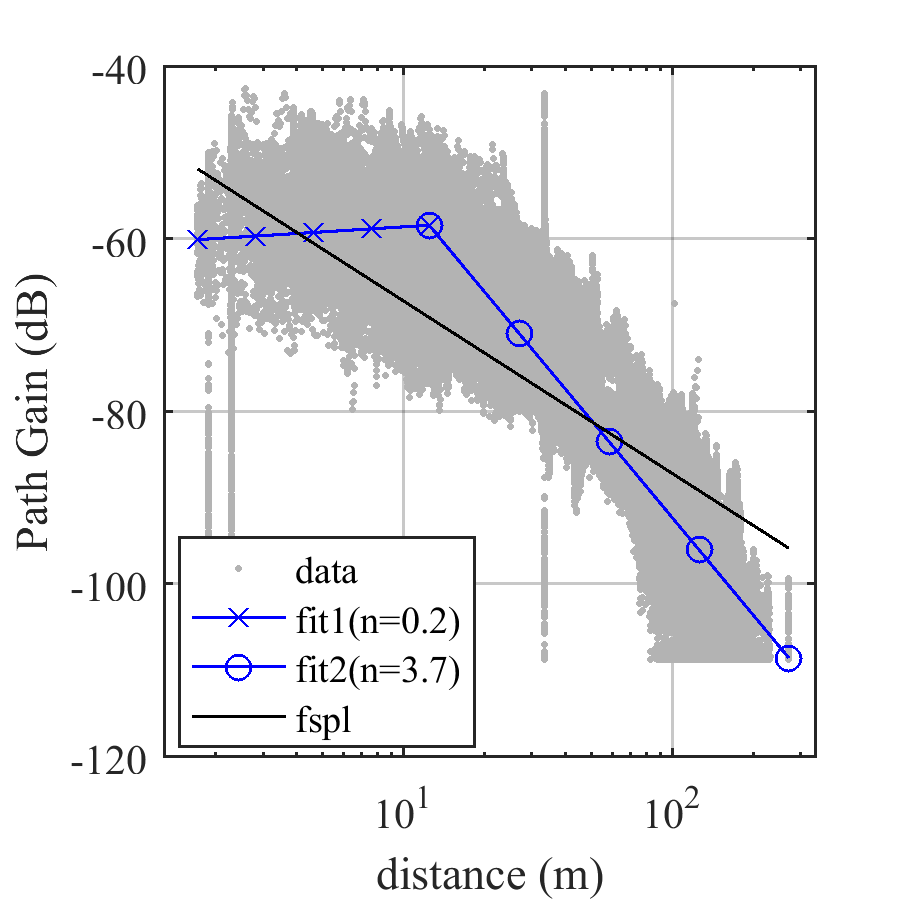
\includegraphics[width=0.6\textwidth]{chapter-intro/images/gain2245}
	\caption{Example of radio propagation path loss for 2245 MHz transmissions within a factory environment.  Reproduced from NIST Technical Note 1951~\cite{Candell2017.NIST1951}}
	\label{intro:pathloss-example}
\end{figure}
 
\paragraph{Multi-path} Objects within the surrounding environment determine the behavior of the waves as they propagate through the environment.  Shown in Fig.~\ref{intro:fig:multipath}is a simplified model of a radio channel. When RF energy is transmitted, it will travel in the direction determined by the antenna gain pattern.  Objects in the environment may obstruct, attenuate, or reflect RF energy.  Reflections contribute to a phenomenon known as multi-path.   Edges of objects may also result in diffraction even if a line-of-sight (LOS) path exists.  At the receiver end, direct path and reflected energy is detected and decoded into useful information if the signal energy was high enough to overcome naturally and artificially occurring noise and interference.  Multi-path reflections may result in significant information loss even if signal power is high.  Multi-path is severe within factories due to the large highly-metallic structures that exists in those environments\cite{Candell2017.NIST1951,Rappaport1991,Remley2008}; therefore, industrial wireless system must anticipate and accommodate these effects.

\begin{figure}
	\centering
	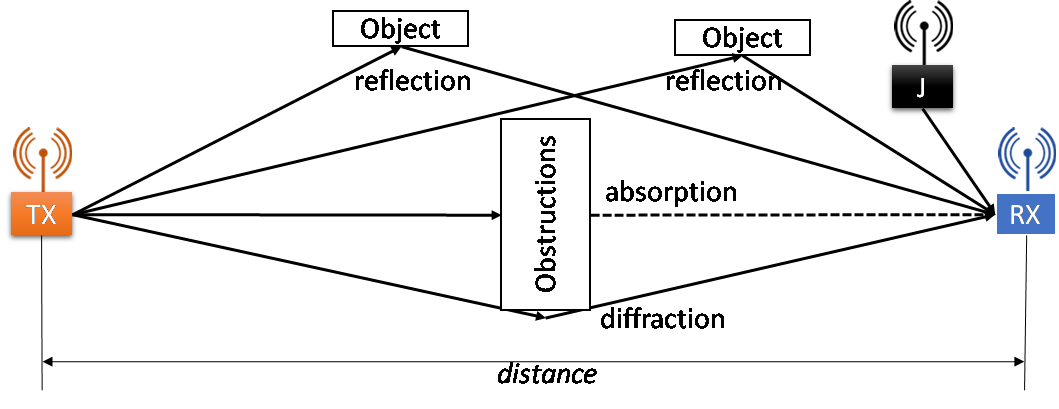
\includegraphics[width=0.6\textwidth]{chapter-intro/images/multipath}
	\caption{Wireless range, obstructions, absorption, reflection, diffraction, and jamming}
	\label{intro:fig:multipath}
\end{figure}

\paragraph{Interference} Electromagnetic interference (EMI) is always present to some degree in a wireless network.  EMI when in the radio frequency spectrum creates a disturbance that disrupts intended communications.  The disturbance can degrade performance by introducing RF energy into the circuits of wireless devices.  When the disturbance is strong enough to overcome the intended signal, communication loss will result.  Sources of EMI include both man-made and natural sources.  Natural radio sources typically will not interfere with network operation as the devices or deployment locations are designed to accommodate some natural interference.  Man-made interference can include other competing radio devices that operate in the same frequency band or nearby in frequency.  Noise from rotating electrical motors can also occur and typically affects radio bands below 400 MHz.  Common interference sources include personal devices such as cell-phones when a Wi-Fi hotspot is enabled.  It can also include non-communication devices such as micro-wave ovens.  EMI can also emanate from intentional radio jammers designed to disrupt communications, and this can be classified as a security issue.

\paragraph{Wireless Protocols Used} Each wireless protocol has been designed with its own target application and ambient environment for performance.  Each protocol is designed with a method for accessing the radio media, organizing data for transmission, methods for receiving transmissions, and recovering from interruptions.   For example, IEEE 802.11 also known as Wi-Fi was designed primarily for home and office use for the transfer of large amounts of data rapidly.  Wi-Fi typically uses 20 to 40 MHz of bandwidth and employs high order modulation and coding schemes.  Wi-Fi works well to transfer files and stream video, and serves well where traditional Ethernet is used; however, Wi-Fi operates within public radio bands and is prone to interference, contention, and non-determinism of response times.  In contrast, other protocols such as WirelessHART and ISA100.11a are designed specifically for industrial wireless sensor networks.  These protocols use low-order modulation schemes with frequency hopping and are by design more resilient to interference.  They also offer substationally better determinism but are limited in data throughput.

\section{Wireless Key Performance Indicators}

Given the challenges described in the previous section, assessing the performance of the wireless system becomes a matter of defining and then measuring key performance indicators (KPI) relevant to the success of a given wireless deployment.  A KPI can be considered a requirement of an industrial system if that KPI is used to specify a condition or capability needed by a stakeholder to solve a problem or achieve an objective within the factory enterprise.  Requirements considerations for designing or implementing a wireless communication system in a factory workcell include latency, reliability, scalability, range, payload size, update rate, operation and implementation cost, security, and system resiliency. These requirements are important aspects of a wireless network~\cite{CandellRW2017}. These requirements have particularly influential roles in implementing a wireless communications system within a factory environment and then assess the success of that wireless deployment.  The following paragraphs define the key performance indicators (which may be considered as requirements) for an industrial wireless system. 

\paragraph{Latency}
Latency is defined as the period of time between information transmission and reception between two actors.  Most non-industrial wireless systems are designed for higher data rates without regard for latency. However, for industrial applications, low latency is an important factor in control-based tasks as transmissions that occur outside of the latency threshold are considered failed transmissions. Industrial applications use smaller packet sizes with precise timings, signifying the criticality of latency.
\begin{definition}[Latency] \label{def:latency}
	The time between transmission of the first bit of information to the time in which that information is received by its intended recipient.
\end{definition}

\paragraph{Reliability}
Industrial functions such as safety transmissions or critical control processes are examples of functions that require an extremely high degree of reliability because a “missing” transmission could have severe consequences to safety, production, and/or equipment integrity. High-reliability in industrial communication is crucial for numerous mission-critical applications. 

\begin{definition}[Reliability] \label{def:reliability}
	The probability of loss of information due to any source of noise or exceeded latency.
\end{definition}

\paragraph{Scalability}
Scale, in an industrial wireless point-of-view, is the number of devices that can be deployed on the network while retaining reliability, speed, and data-rate at set requirements. Scalability is important for dynamic networks where devices come-in and go-out of use. One distinct advantage of wireless communications is the ease with which nodes can be added to the network without the need for laying wire or cable.
\begin{definition}[Scale] \label{def:scale}
	The number of participating devices within a network.
\end{definition}

\paragraph{Range}
Range is the maximum distance to which a wireless link can extend while maintaining all other requirements. In general, as the distance of the wireless link increases, the channel losses increase and the signal power between nodes decreases. Excess range affects the reliability and latency of transmission.
\begin{definition}[Range] \label{def:range}
	The maximum distance to which a wireless link can extend while maintaining all other requirements
\end{definition}

\paragraph{Payload Size}
Payload size is the size, in bytes, of the information portion of a transmission; however, the payload excludes header, framing, and error-correction information. Differentiating the payload size from the overall individual packet size allows the designer to ascertain the size of the information portion of the transmission. Many industrial applications, such as safety and control applications, the payload size is small.
\begin{definition}[Payload Size] \label{def:payloadsize}
	The informational length of information to be transmitted not including all overhead associated with the protocol used for transmission.
\end{definition}

\paragraph{Update Rate}
Certain manufacturing applications require higher update rates to achieve desired workcell performance. A wireless network must support the required update rates needed by all the applications on that wireless network. For example, a force feedback control application that utilizes a wireless force-torque sensor may require 125 Hz sample rate. An example of such an application may be found in reference~\cite{Candell_ISIT_2019}. Update rate is an important factor that impacts the deployment and configuration of wireless networks and it dictates the effectiveness of frequency planning~\cite{Candell2018.IWSGuide}.
\begin{definition}[Update Rate] \label{def:updaterate}
	Rate of transmission for a particular process variable.
\end{definition}

\paragraph{Operation and Implementation Costs}
A consideration for implementing industrial wireless communications is the cost savings. For a wireless communications system, there is no need to install and, later, replace cabling due to degradation and wear. In wireless communications, redundancy can be achieved without cables. Wireless communications require lower labor costs as remote monitoring and control extend the ability to monitor and manage remote sites; onsite personnel is unnecessary. Electricity cost is lower for wireless installations, due to the relatively low power draw of wireless communications.

\paragraph{Security}
Security in wireless communications is not equivalent to security in wired communications in that wireless networks offer a different potential for exploitation; wireless uses air for communication which provides easier access to remote foreign actors. Along with the threat of remote jamming, there exists the possibility, absent adequate security protection, that wireless networks could be accessed if the keys to the public-key cryptography are discovered and encrypted transmissions are revealed. Wireless for industrial applications must be reliant to security related threats as the loss of communication can be costly and may damage equipment or personnel. Detailed requirements for wireless security are not discussed further in this report but more information can be found in~\cite{Stouffer2015}.

\paragraph{System Resiliency}
Overall system resiliency in a factory environment must be considered as issues with networking may lead to unnecessary inefficiency. For example, if power is disrupted, a network must be able to re-establish connectivity within seconds. Intelligent applications may also be required to overcome network communication issues. Achieving a resilient network is not trivial as current wireless device may require long periods of time to re-establish connections within the network.  For example, mesh networks based on low-data-rate protocols can often take minutes to reestablish an operational network after an intermittent loss of power.  System resiliency is outside the scope of this report; however, system resiliency issues such as recovery time after power loss must be considered in the design of wireless technology for use in factory workcells.

\paragraph{Power and Battery Life}
Often overlooked is the power efficiency of wireless devices.  In factories in which power is readily available such as in a workcell or on a mobile cart platform, power efficiency is not often considered.  In scenarios where devices are deployed over large distances such as in a oil refinery or water purification plant, battery life becomes important.  Battery life can also be important for large scale deployments in factories with thousands of devices.  In those scenarios, the frequency of battery change or failure can drive costs substantially.  Therefore, power efficiency and the impact of design factors on battery life can be equally as important as reliability in a deployment. 


These requirements vary greatly depending on the class of industrial application and much work has been done to try to make sense of the classes of applications and there subsequent requirements.  An illustrative perspective of these is given in Fig.~\ref{intro:fig:wirelesspecs} showing both typical and worst case specifications and how each relate.  


\begin{figure}[!tbp]
	
	\centering
	\begin{subfigure}{.8\textwidth}
		\centering
		% include first image
		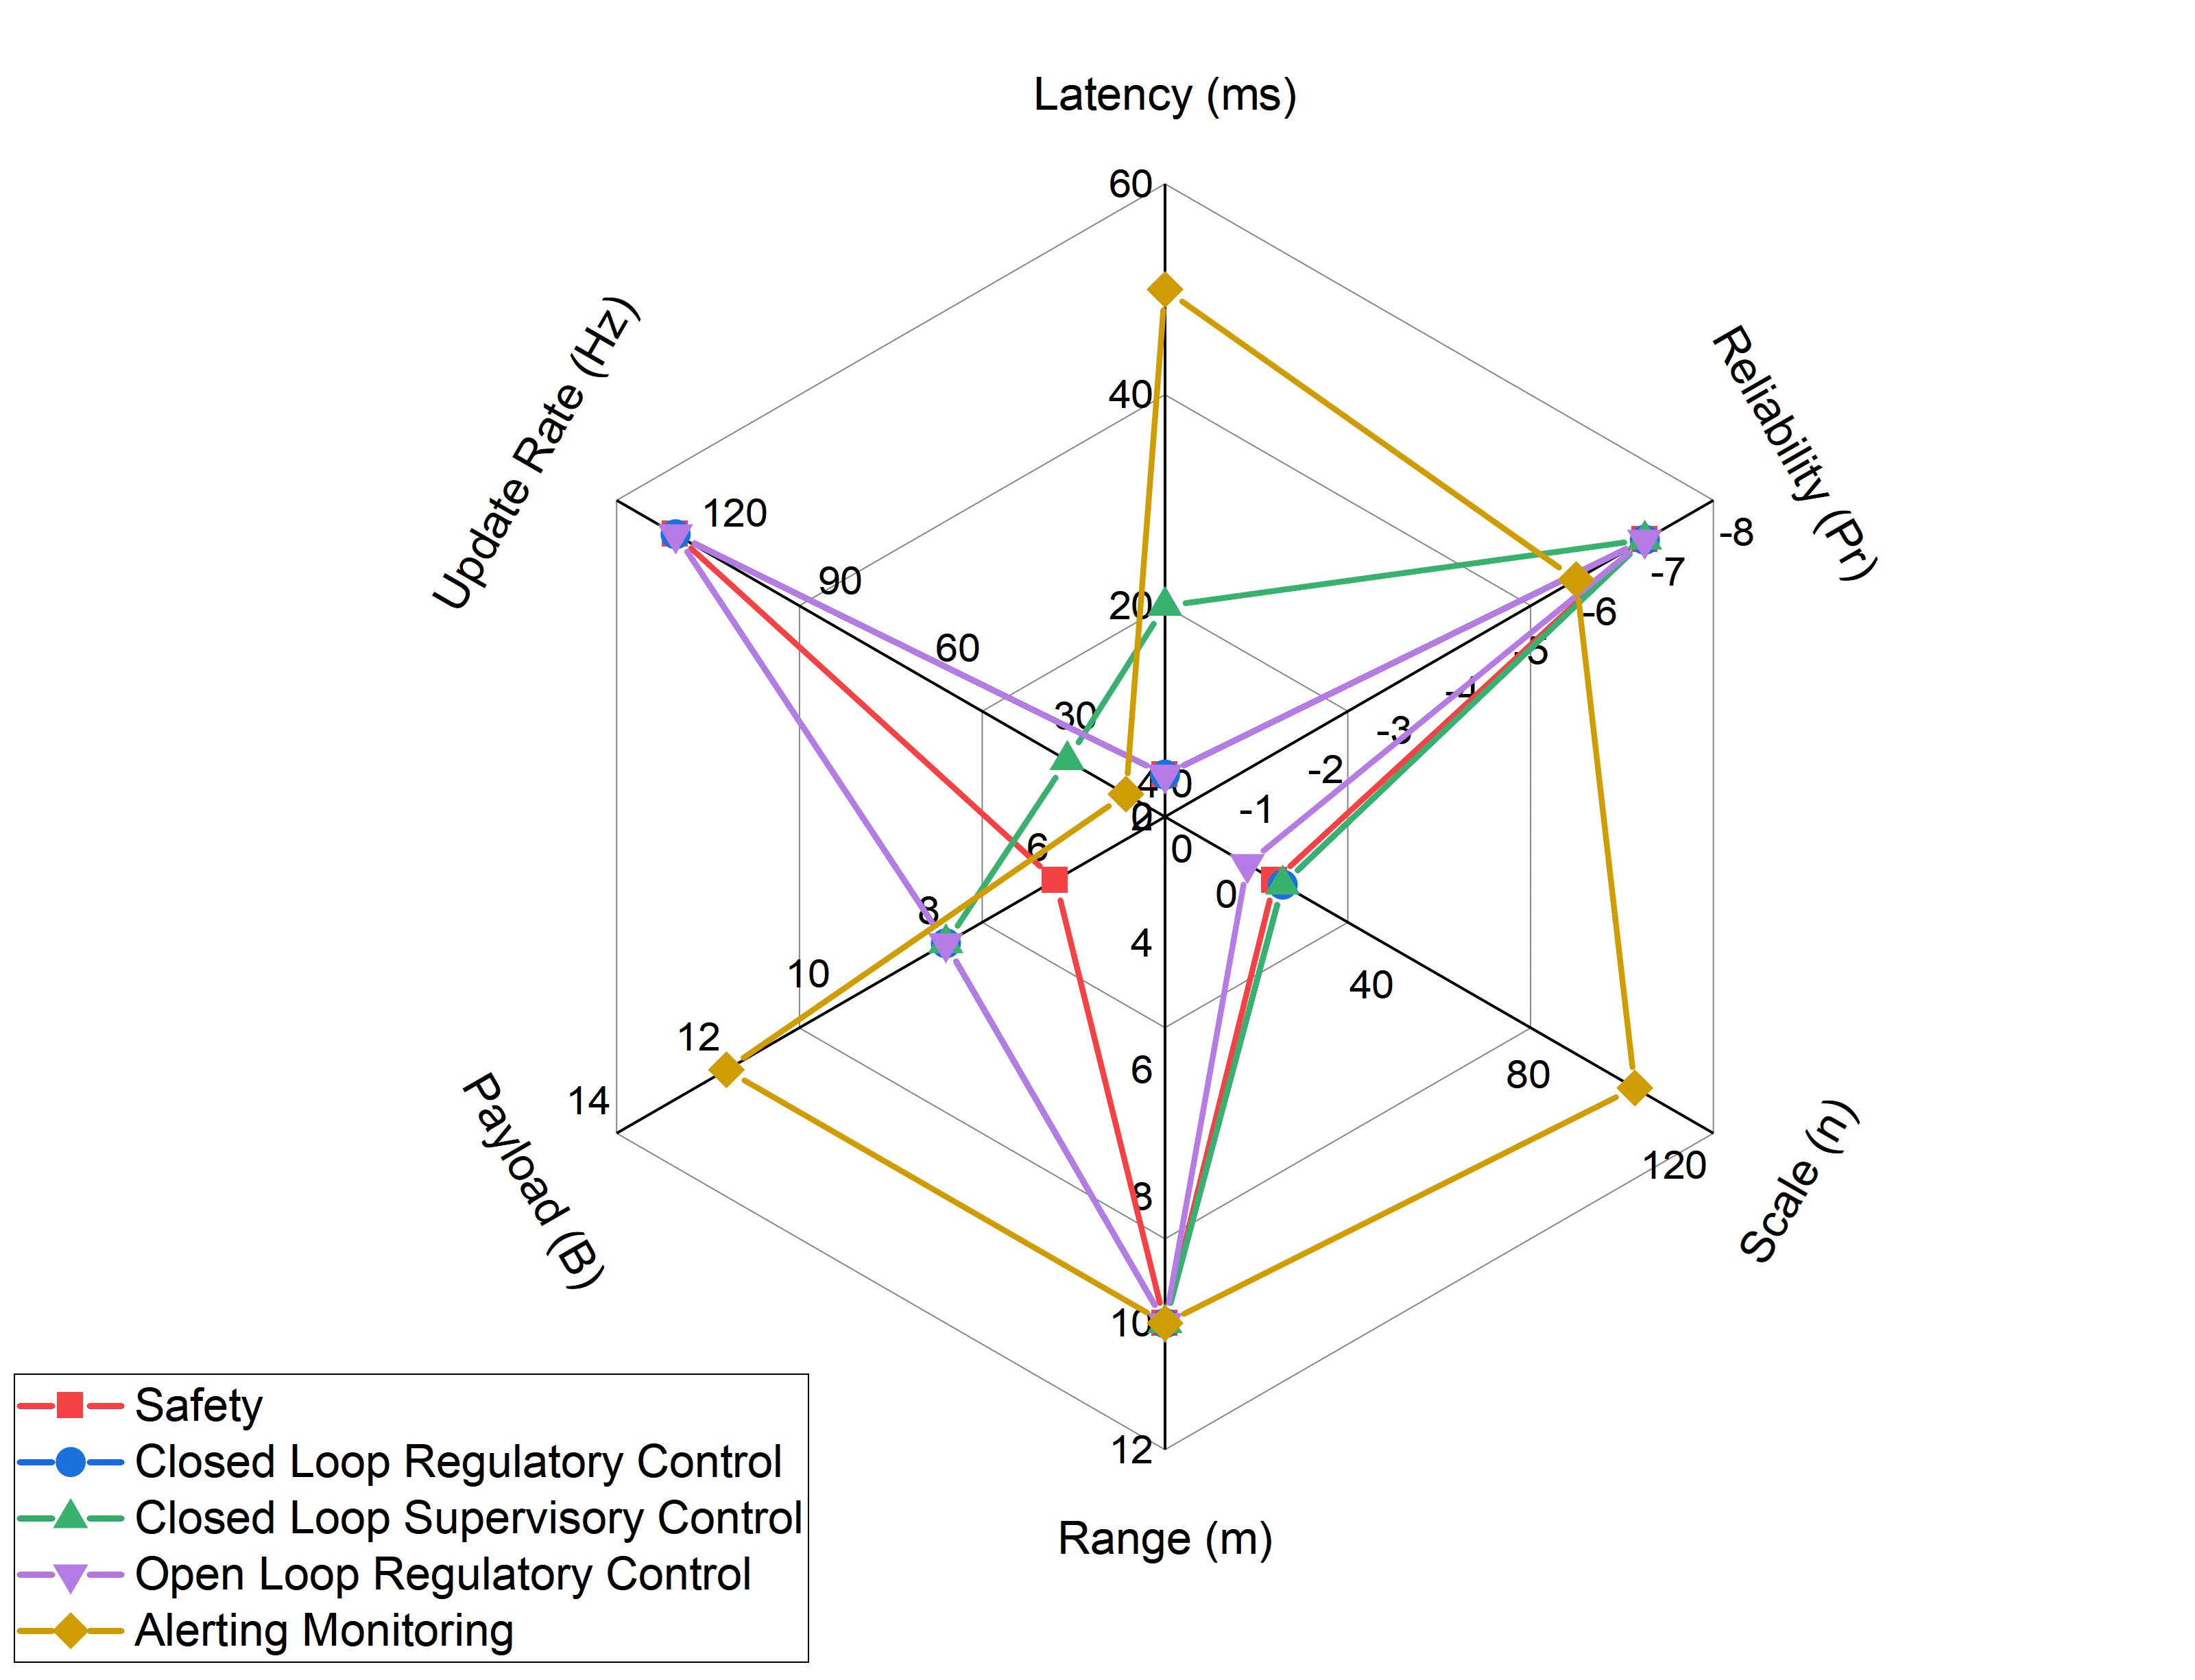
\includegraphics[width=.95\textwidth]{chapter-intro/diagrams/TypicalSpecs}  
		\caption{Typical}
		\label{intro:fig:typicalspecs}
	\end{subfigure}
	\begin{subfigure}{.8\textwidth}
		\centering
		% include second image
		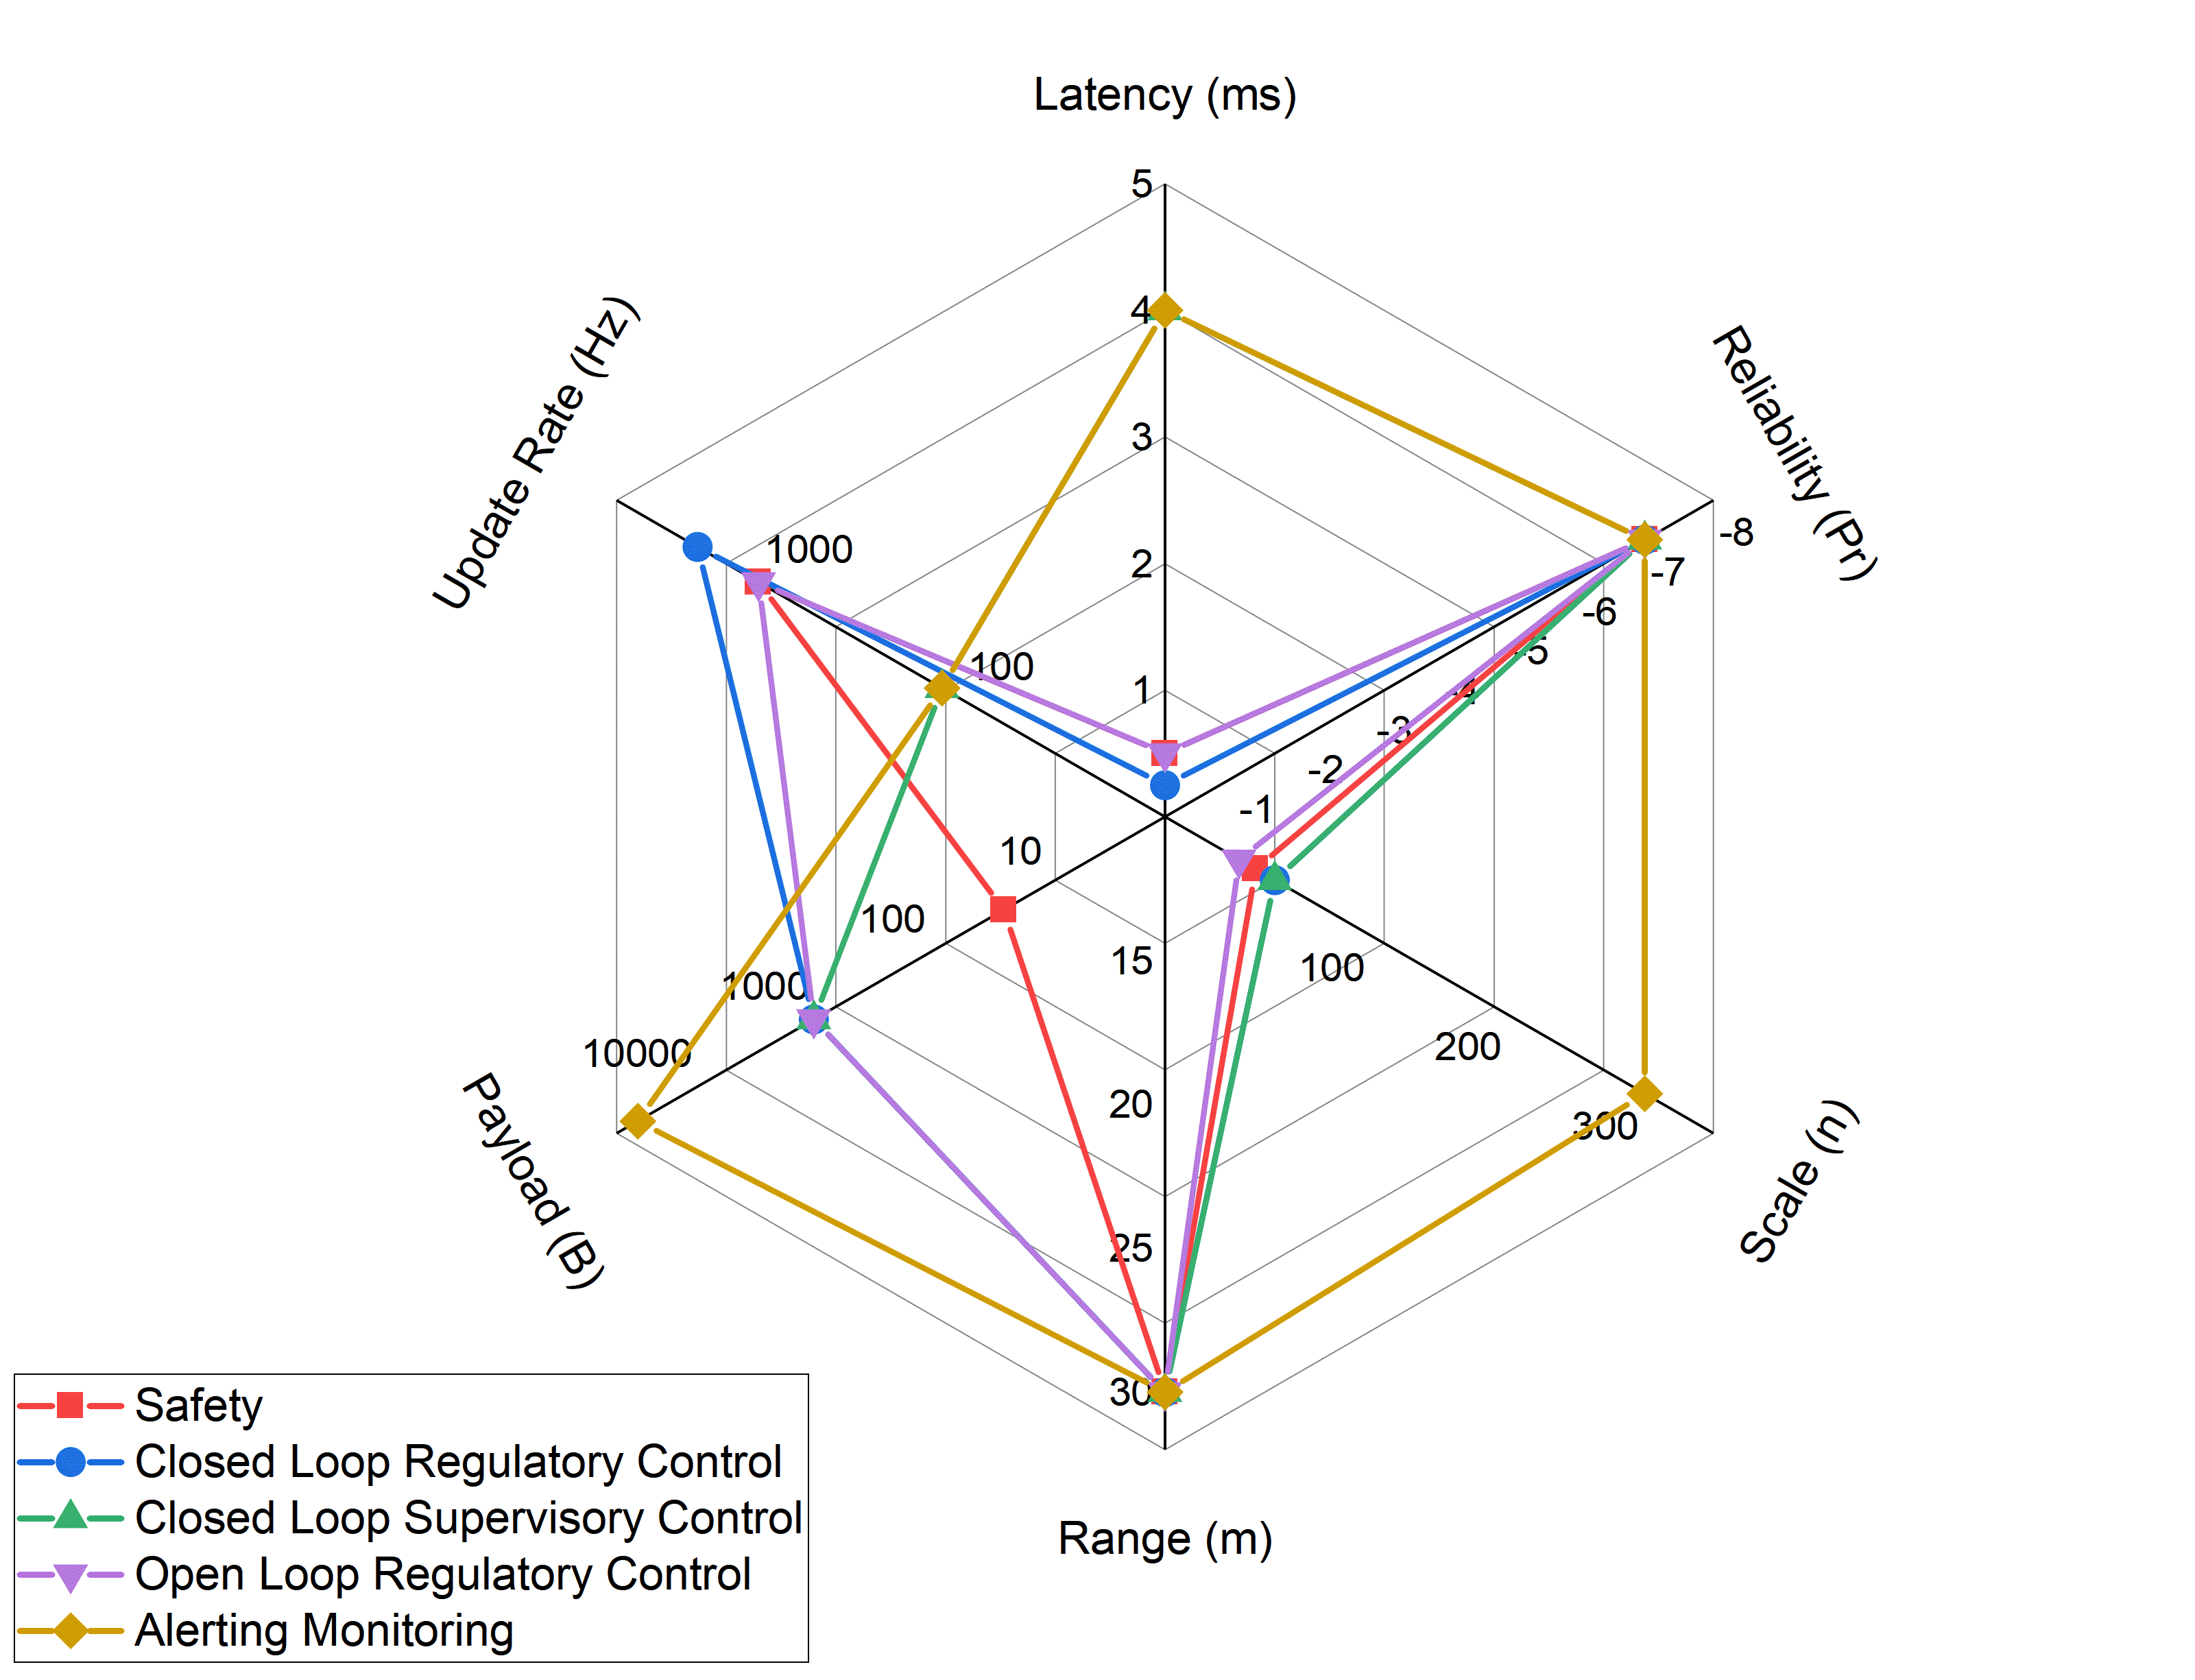
\includegraphics[width=.95\textwidth]{chapter-intro/diagrams/WorstSpecs}  
		\caption{Worst Case}
		\label{intro:fig:worstspecs}
	\end{subfigure}
	\caption{
		Typical ~\protect\subref{intro:fig:typicalspecs} and Worst Case ~\protect\subref{intro:fig:worstspecs} key performance indicators for industrial wireless use cases presented in~\cite{Montgomery2019}.
	}
	\label{intro:fig:wirelesspecs}	
	
\end{figure}



%\section{Performance Evaluation}
%
%The focus of the research presented in this body of thesis is performance estimation of both the netwpork and physical 
%
%Present the TESTBED!!!
%
%A clearer concept of the requirements will not only allow for the development of realistic wireless systems, but it is also essential in the construction of more accurate models, the conduct of more effective testing, and better analysis the performance measurement data that results.
%
%First understanding the technical landscape: components, interfaces, and constraints
%
%Next setting up a framework for performance evaluation: use case definition, testbed abd data capture, organization of data captured, 
%
%Analysis methods for the captured data: data cleaning, curation, and application of the graph database
%
%Application of machine learning as an example and how different algorithms performance to inferring an important metric in industrial wireless, i.e., signal to interference level
%
%Performance is often done as a before and after; however some effort has been made to standardize test methods~\cite{Candell2015, Candell2017IWW}

\section{Contribution Summary and Thesis Organization}

\begin{figure}[!tbhp]
	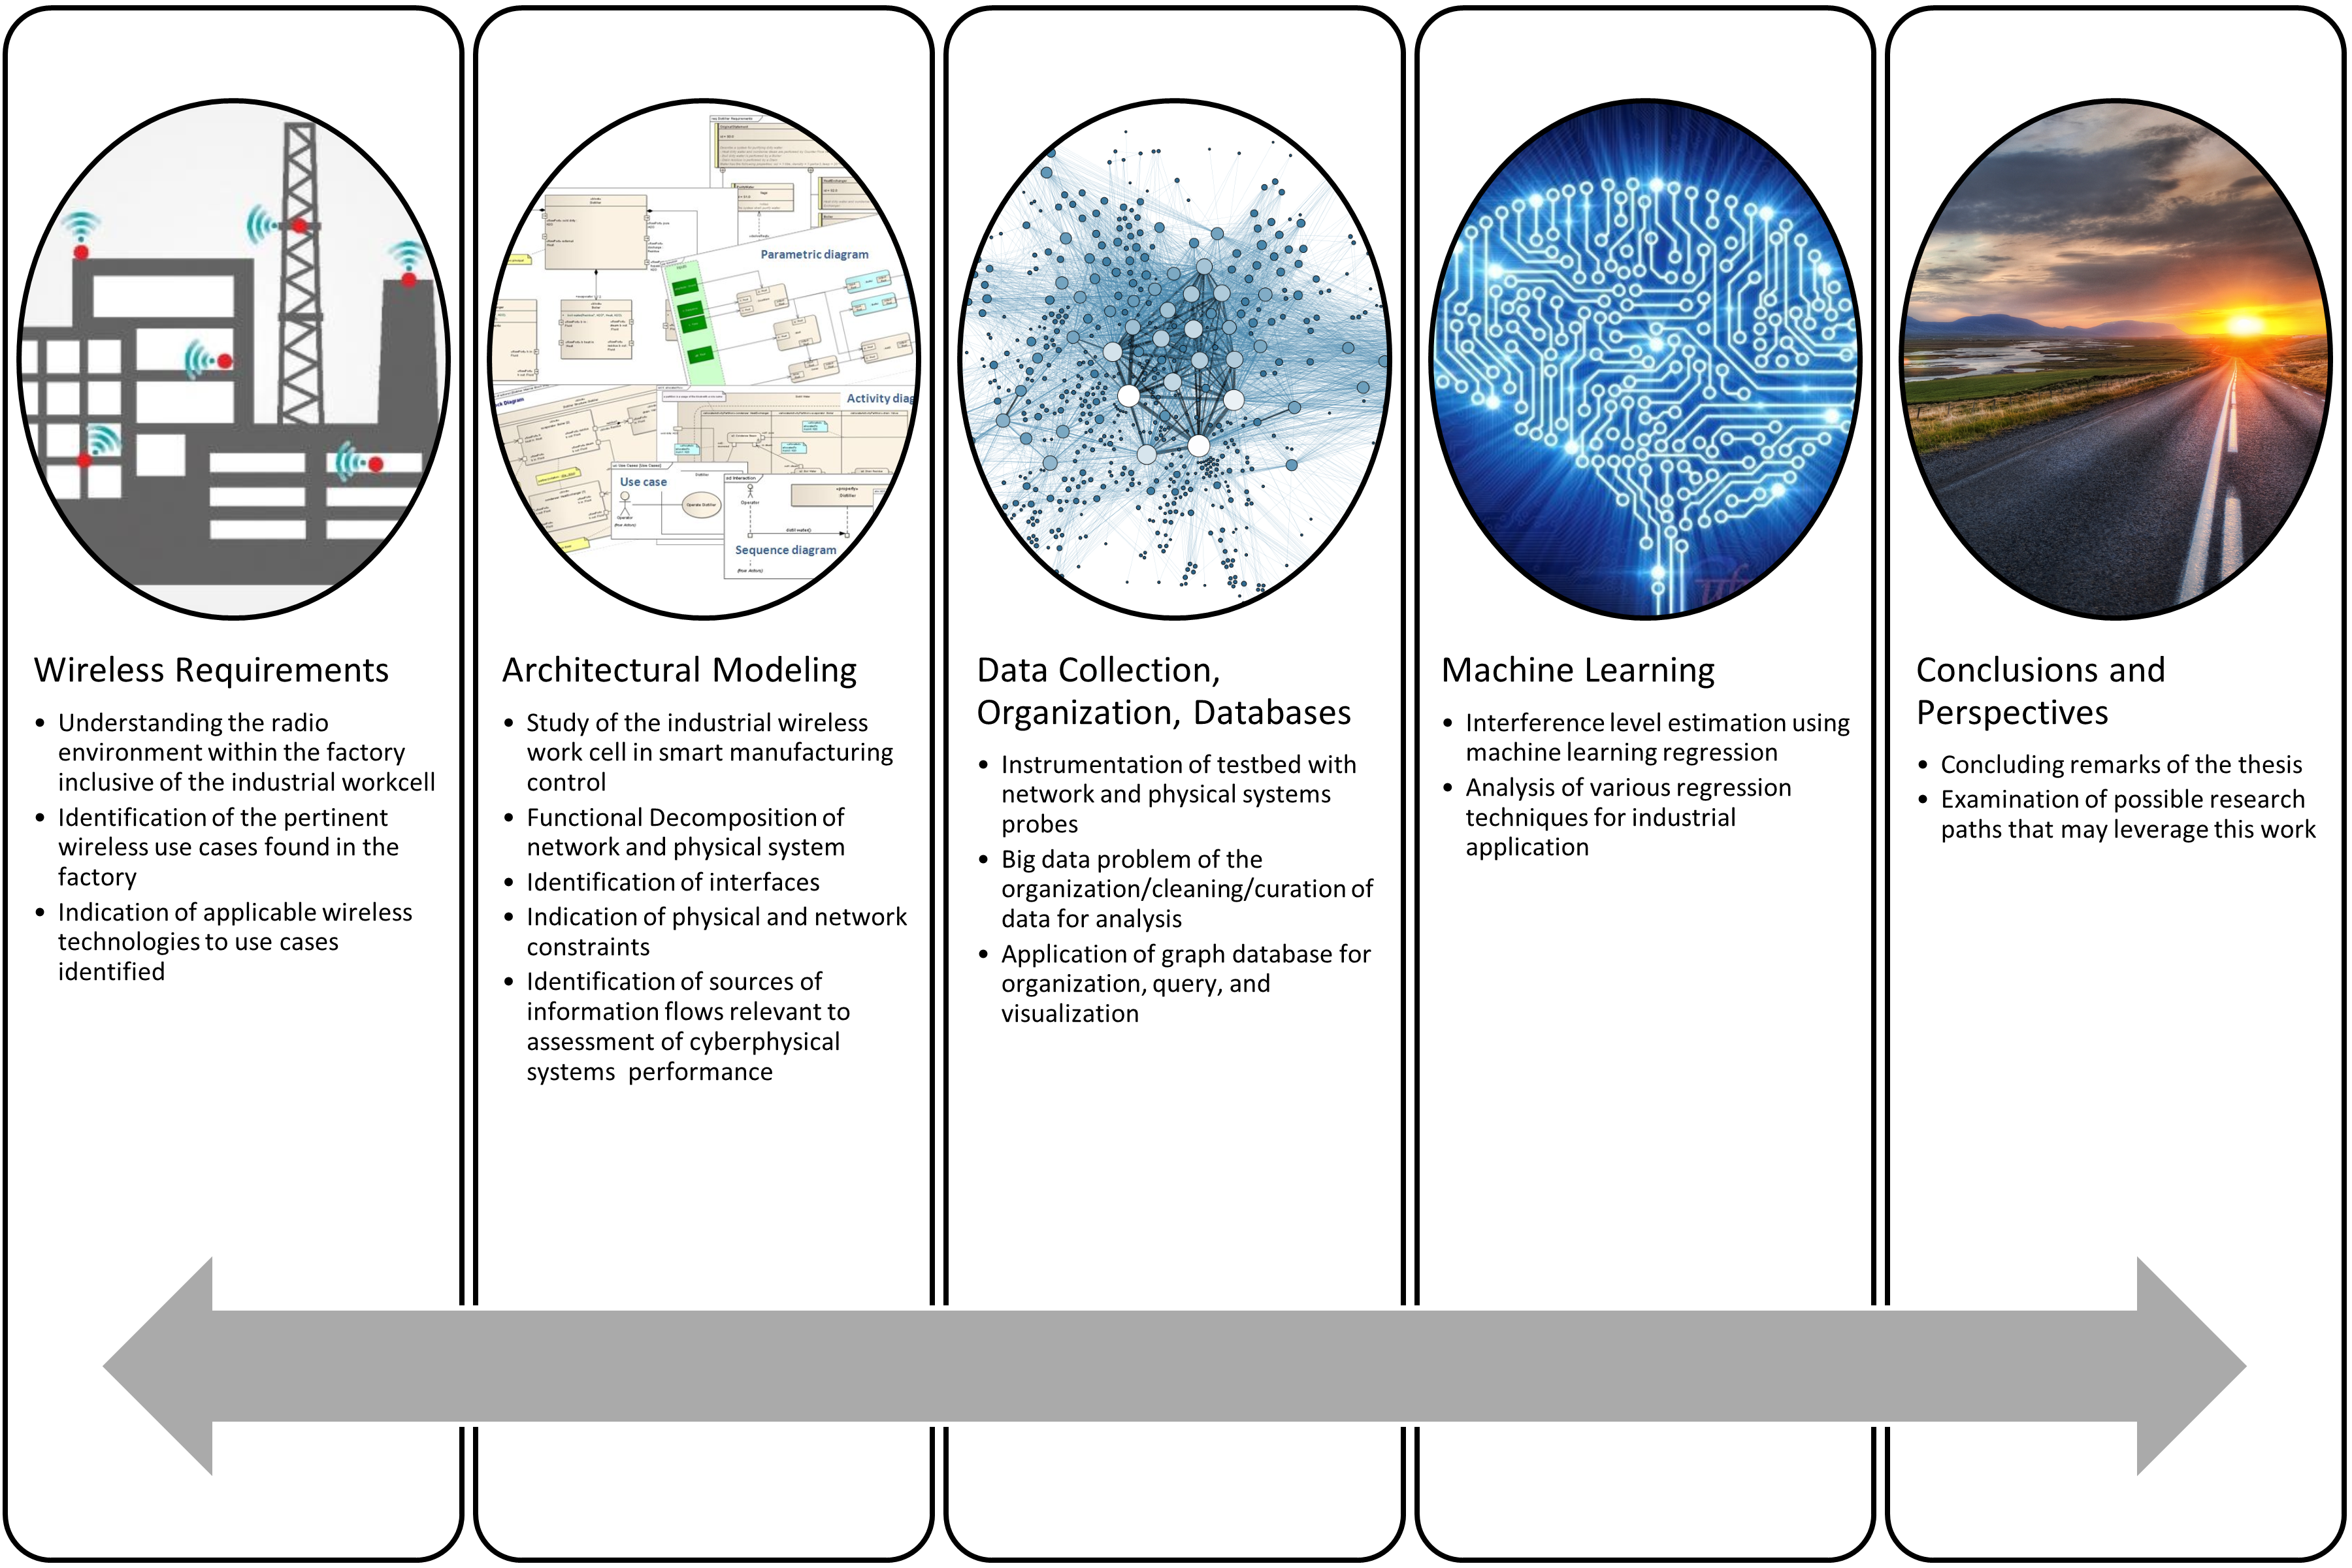
\includegraphics{chapter-intro/images/contributions}
	\caption{Contribution areas and organization of this thesis.}
	\label{fig:intro:contr-org}
\end{figure}

This thesis is presented in three major parts.  The first part, Part~\ref{part:context}, \textit{Context and Problem Statement} provides a historical introduction to the context of smart manufacturing.  It presents the premises of industrial wireless technology, key challenges to using wireless within a factory environment, and the accepted indicators that are currently used in the application of wireless within factory environments. In Part~\ref{part:context}, the existing state of the art is also presented in Chapter~\ref{chapter:soa}.  This state of the art includes a discussion of the industrial wireless technology landscape, standards, and a tentative mapping of those technologies to application domains.  A discussion of the systems modeling approaches is then provided with a focus on the Systems Markup Language (SysML).  A discussion of approaches to the use of databases follows.  In Part~\ref{part:techical}, \textit{Thesis Contributions}, the technical contributions of this thesis are presented, providing a detailed discussion of the four major contributions of this thesis work.  The thesis contributions are presented as follows:

%\begin{description}
%	\item[Requirements] \cite{CandellRW2017}, \cite{Montgomery2019}, \cite{Candell2018.IWSGuide} An examination of the wireless technology landscape is conducted.  Existing and future wireless technologies are assessed for their appropriate applicability to industrial use cases. 
%	
%	\item[Modeling] \cite{Candell2019ASR.SYSML}, \cite{Candell2018SysML.JRES}, \cite{Candell2018SysML.GitHub} In an effort to better understand the architectural composition of the workcell using industrial wireless communication, modeling techniques are used to identify and decomposed the parts, interfaces, and data flows.  SysML is adopted for this process and a proposed modeling library is created and presented.  The model with conceptual diagram is made publicly available independent of the tool that was used to create the model.
%	
%	\item[Application of Graph Database] \cite{CandellISIT2020.Conf} A method is developed for collecting, cleaning, organizing, and presenting the cyberphysical performance indicators of experiments run within the NIST Industrial Wireless Testbed. The method developed utilizes the Neo4j graph database and is presented as a novel approach as compared to traditional approaches using relational database, spreadsheets, and raw file processing.
%	
%	\item[Machine Learning] \cite{CandellISIE2019.Conf}, \cite{CandellISIE2019.Conf.Data}, \cite{CandellIJAMT2020.Jrml} A machine learning technique is developed and applied to the prediction of signal-to-interference levels within a wireless factory workcell network employing a robot arm within a force-seeking apparatus.  The machine learning method allows a trained network to accurately determine the signal-to-interference level using the physical state of the robot arm rather than the state of the wireless link itself.
%\end{description}

		\begin{description}
	
	\item[Requirements] \cite{CandellRW2017} \cite{Montgomery2019} \cite{Candell2018.IWSGuide} \cite{ieeeMagazine2018} An examination of the wireless technology landscape is conducted.  Existing and future wireless technologies are assessed for their appropriate applicability to industrial use cases. In~\cite{Candell2018.IWSGuide}, the authors produced a major contribution for the manufacturing industry to effectively design and deploy industrial wireless networks used for sensing, control, monitoring, and surveillance.  In ~\cite{ieeeMagazine2018}, the guidelines are presented to the academic community as a peer-reviewed article.
	
	\item[Modeling] \cite{Candell2019ASR.SYSML} \cite{Candell2018SysML.JRES} In an effort to better understand the architectural composition of the workcell using industrial wireless communication, modeling techniques are used to identify and decomposed the parts, interfaces, and data flows.  SysML is adopted for this process and a proposed modeling library is created and presented.  The model with conceptual diagram is made publicly available independent of the tool that was used to create the model.
	
	\item[Application of Graph Database] \cite{CandellISIT2020.Conf} \cite{GraphDB.JCISE.Journal} A method is developed for collecting, cleaning, organizing, and presenting the cyber-physical performance indicators of experiments run within the NIST Industrial Wireless Testbed. The method developed utilizes the Neo4j graph database and is presented as a novel approach as compared to traditional approaches using relational database, spreadsheets, and raw file processing.
	
	\item[Machine Learning] \cite{CandellISIE2019.Conf} \cite{Candell2020.Jrnl.Access} A machine learning technique is developed and applied to the prediction of signal-to-interference levels within a wireless factory workcell network employing a robot arm within a force-seeking apparatus.  The machine learning method allows a trained network to accurately determine the signal-to-interference level using the physical state of the robot arm rather than the state of the wireless link itself.
	
\end{description}

Subsequently, in~\cite{Candell.PLMConf2020}, we present a new industrial wireless testbed design that motivates academic research and is relevant to the needs of industry. The testbed is deigned to serve as both a demonstration and research platform for the wireless workcell. The work leverages lessons learned from past incarnations that included a dual robot machine tending scenario and a force-torque seeking robot arm apparatus. This version of the testbed includes computational and communication elements such that the operation of the physical system is noticeably degraded under the influence of radio interference, competing network traffic, and radio propagation effects applied within the lab. Key performance indicators of the testbed are selected and presented which include communication, computational, and physical systems indicators. This new testbed will be used to perform future research motivated by this thesis.

An additional contribution is cited here~\cite{MSEC2019-2896}.  In this work, we have designed, constructed, and executed an experiment in which a typical two-dimensional gantry apparatus was controlled by a local controller which received G-code commands wirelessly over a Wi-Fi network. The industrial wireless channel was replicated using a radio frequency (RF) channel emulator where various scenarios were considered and various wireless channel parameters were studied. The movement of the gantry system tool was tracked using a vision tracking system to quantify the impact of the wireless channel on the system performance. Numerical results were presented including the total run time of an industrial process and the dwell times at various positions through the process. This contribution is not discussed within the thesis.

Finally, this thesis concludes in Part~\ref{part:conclusion}.  Our concluding remarks and recommended future direction are provided.





%\part{State of the Art}\label{part:soa}

\chapter{State of the Art}\label{chapter:soa}

\chapterintro*

This chapter present the reader with background conducted during the thesis investigations. The chapter is presented as a "State-of-the-art" but it can also be considered as a a compilation of the related work previously performed by other interested researchers within the field.  The content, therefore, of this chapter contains a summary of the previous works discovered for the contributions presented in Part~\ref{part:techical}.  The chapter is divided into three main sections: 1) an exploration of industrial wireless requirements with a mapping of those requirements to existing and future wireless technologies; 2) system modeling of the factory with specific mention of the wireless workcell; 3) the organization of data for the collection and analysis of performance data of \glspl{cps} found in factory workcells; and, finally, 4) applications of machine learning for the prediction of wireless network performance within factory workcells. 

\section{Industrial Wireless Requirements Space}\label{sec:requirements-space}

The use of \glspl{iwn} has been studied in many works in the literature and industry. However, no comprehensive survey of the holistic problem space of industrial communications has been performed.   The following chapter provides background into the evolving landscape of industrial wireless requirements.  It should be noted that the requirements perspective is often influenced by hype in the marketplace, and often the requirements that are stated are unrealistic or impossible to meet within reasonable price points.  First, a literature review has been provided which was the result of the work presented in~\cite{CandellRW2017}.  This literature review will be followed by an elaborated perspective provide in NIST 300-8~\cite{Montgomery2019} of which the candidate took a lead role in leading, contributing, and writing.  Within that work, a picture of the wireless requirements landscape is provided based on inputs from the \gls{isa} and the \gls{etsi}.  The work then provides a more distilled view of the requirements perspective with rationale.  This distilled perspective serves as both a state of the art of industrial user requirements viewed by \gls{etsi} and \gls{isa}, but it also serves as a major contribution in that it provides validated requirements that are usable to build realistic and functional wireless systems.  This is ultimately the goal of performing a rigorous review of the requirements landscape and producing saner perspective.  A clearer concept of the requirements will not only allow for the development of realistic wireless systems, but it is also essential in the construction of more accurate models, the conduct of more effective testing, and better analysis of the performance measurement data that results.


\subsection{Literature Review}\label{sec:litreview:academia}

This section provides an overview of the literature review conducted for the work performed in~\cite{CandellRW2017} in which the broad landscape of industrial wireless use cases were considered and then matched with potentially applicable wireless technologies that existed or were in the process of standardization or development.  

In \cite{Galloway2013}, the authors introduce a comparison between the commercial and industrial communications networks where an industrial network has been divided to five different levels. These levels include field equipment, controller, application, supervisory, and external networks. The differences in requirements between different levels are discussed. 

Three types of information are considered which are control, diagnostic, and safety information as described in \cite{Moyne2007}.  Within this reference, the authors categorize the types of industrial control network their applications within a reconfigurable factory testbed developed at the University of Michigan. While all these levels of industrial networks are mentioned in \cite{Galloway2013}, the article focuses only on the manufacturing and instrumentation communications and does not consider other types of communications networks that exist in industrial environments. 

In \cite{What2017}, and online tutorial describing industrial protocol, three levels of communications are considered which are device, control, and information levels. Current wired industrial technologies for these levels are discussed briefly. 

In \cite{Danielis2014}, provides a survey on real-time communication using Ethernet technologies in industrial automation environments.  In this work, the communication between field devices was studied where the requirements for a large number of nodes may not be achieved. The use of fieldbus solutions limit the scalability and resilience and hence industrial Ethernet capabilities are introduced in this article. While limited insight into wireless solutions is provided, the article provides insight into the key performance criteria for real-time protocols in general.

Moreover, in \cite{Connectivity}, the communication for monitoring and control operations is discussed and an introductory discussion for wireless adoption for these use case classes is provided. A comparison between fieldbus technologies, industrial Ethernet, and wireless solutions is performed. The author discusses the use of \gls{wifi}, Bluetooth, ZigBee, and WirelessHART technologies in industrial applications. 

In~\cite{Ikram2010} the authors consider the industrial communications networks requirements in process automation specifically at field devices level. The authors provide a survey of opportunities, requirements, concerns and challenges of wireless in process automation, the relative standings of existing short-range wireless network technologies, and their perceived shortcomings. The authors also provide an examination of emerging industrial wireless standards which are designed to address the harsh performance requirements of the process industry given the ambient environment of those factories.

Finally, in~\cite{QUEIROZ201796}, the authors perform and expansive survey on \glspl{wsn} and provide a systemic mapping of research in this area.  The authors show trends within the research community and demonstrate the importance of developing new protocols that are resilient to the harsh transmission media found in factories.  The authors also indicate that a star topology of \glspl{iwn} may be the more appropriate selection for most latency and reliability constraints.


\subsection{Industry Requirements Perspectives}

In the following discussions, a presentation of different perspectives of various user requirements provided by industry is given based on industry reports from two noteworthy organizations.  These perspectives differ from the perspectives provided by the academia in Section~\ref{sec:litreview:academia} in that the contributors of these reports were individuals working directly within factory organizations or suppliers of products and services used by factory controls engineers.  The first discussion in Section~\ref{sec:litreview:isa} focuses on the requirements work performed by the standards organization, the International Society of Automation.  The second discussion given in Section~\ref{sec:litreview:etsi} focuses on work performed by \gls{etsi} regarding high-reliabilty, low-latency communications requirements for industrial applications, and in particular for the 5th generation wireless evolution known as \gls{5g}.  The third discussion provided in Section~\ref{sec:litreview:industry} while an academic article was the result of research performed by engineers developing wireless products for high-performance wireless networks used to control industrial operations by latency constraints within the microsecond range.  Finally, a consolidated and actionable perspective is provided which serves as both background material and our contribution.  The consolidated perspective of the requirements and implied architecture were useful in the development of the \gls{sysml} model presented in Chapter~\ref{chapter:sysml}.

\subsubsection{ISA Requirements Perspective}\label{sec:litreview:isa}

The \gls{isa} is a non-profit standardization body that produced Wireless User Requirements for Factory Automation [10]. The \gls{isa} provided classes that categorized industrial applications and use cases, and assigned wireless user requirements for latency, jitter, and \gls{bler}. Table~\ref{soa:isa-classes}, adapted from~\cite{ISATR100-2011}, provides usage classes with their respective descriptions; these classes are grouped by domain, in factory automation use cases. It is important to note that the “Factory Automation Use Cases” column references “Clauses” which describe applications in the usage classes in detail and are not discussed in this report. The Clauses discuss various industrial applications and such applications apply to different classes. For example, the \gls{reef} for Class 1, track-mounted equipment and rotary equipment for Class 2, track-mounted equipment and rotary equipment, but with a human in the loop for Class 3; torque and gauge tools, mobile material containers, mobile high value assets (molds, dies, etc.), and mobile test and calibration fixtures for Class 4. Note that the report references similar applications for Class 4 as for Class 5, except with the purpose of logging, downloading, and uploading; also note that Class 0 presented in this thesis, was not discussed in the report. The \gls{isa} requirements, adapted in Table~\ref{soa:isa-reqts-persp}, define \gls{bler} as the probability of an erroneous block received at the application layer. It should be noted that all usage classes have a requirement of $10^{-9}$ \gls{bler}, an assumed requirement, without justification, in the ISA’s report. 

% Table generated by Excel2LaTeX from sheet 'ETSI and ISA'
\begin{table}[!tb]
	\centering
	\caption{ISA Descriptions of Wireless Requirements Classes}
	% Table generated by Excel2LaTeX from sheet 'ETSI and ISA'

	\begin{adjustbox}{width=\columnwidth,center}
		
	% Table generated by Excel2LaTeX from sheet 'ETSI and ISA'
	\begin{tabular}{|l|l|p{10.645em}|p{10em}|}
		\toprule
		\multicolumn{1}{|p{6.355em}|}{\textbf{Domain}} & \multicolumn{1}{p{13.07em}|}{\textbf{Usage Class}} & \textbf{Description} & \textbf{Factory Automation Use Cases} \\
		\midrule
		\multicolumn{1}{|l|}{\multirow{2}[2]{*}{Safety}} & \multicolumn{1}{l|}{\multirow{2}[2]{*}{Class 0:  Emergency action}} & \multirow{2}[2]{*}{Always critical } & \multicolumn{1}{l|}{\multirow{2}[2]{*}{}} \\
		&       & \multicolumn{1}{l|}{} & \multicolumn{1}{l|}{} \\
		\midrule
		\multicolumn{1}{|l|}{\multirow{8}[6]{*}{Control}} & \multicolumn{1}{l|}{\multirow{2}[2]{*}{Class 1:  Closed loop regulatory control}} & \multirow{2}[2]{*}{Often critical } & \multirow{2}[2]{*}{Clause 5.3 } \\
		&       & \multicolumn{1}{l|}{} & \multicolumn{1}{l|}{} \\
		\cmidrule{2-4}      & \multicolumn{1}{l|}{\multirow{3}[2]{*}{Class 2:  Closed loop supervisory control}} & \multirow{3}[2]{*}{Usually non-critical } & Clause 5.4  \\
		&       & \multicolumn{1}{l|}{} & Clause 5.5  \\
		&       & \multicolumn{1}{l|}{} & \multicolumn{1}{l|}{} \\
		\cmidrule{2-4}      & \multicolumn{1}{l|}{\multirow{3}[2]{*}{Class 3:  Open loop control}} & \multirow{3}[2]{*}{Human in the loop } & Clause 5.4  \\
		&       & \multicolumn{1}{l|}{} & Clause 5.5  \\
		&       & \multicolumn{1}{l|}{} & \multicolumn{1}{l|}{} \\
		\midrule
		\multicolumn{1}{|l|}{\multirow{9}[4]{*}{Monitoring }} & \multicolumn{1}{l|}{\multirow{5}[2]{*}{Class 4:  Alerting}} & Short-term operational  & Clause 5.6  \\
		&       & consequence (e.g., event-based  & Clause 5.7  \\
		&       & maintenance)  & Clause 5.8  \\
		&       & \multicolumn{1}{l|}{} & Clause 5.9  \\
		&       & \multicolumn{1}{l|}{} & \multicolumn{1}{l|}{} \\
		\cmidrule{2-4}      & \multicolumn{1}{l|}{\multirow{4}[2]{*}{Class 5:  Logging, Downloading, and Uploading}} & No immediate operational  & Clause 5.6  \\
		&       & consequence (e.g., history  & Clause 5.7  \\
		&       & collection, sequence of events,  & Clause 5.8  \\
		&       & preventive maintenance)  & Clause 5.9  \\
		\bottomrule
	\end{tabular}%

	\end{adjustbox}

	\label{soa:isa-classes}%
\end{table}%


% Table generated by Excel2LaTeX from sheet 'ETSI and ISA'
\begin{table}[!tb]
	\centering
	\caption{ISA Wireless Requirements Perspective}
	\label{soa:isa-reqts-persp}%

	% Table generated by Excel2LaTeX from sheet 'ETSI and ISA'
	\begin{tabular}{|p{10.57em}|p{5.855em}|p{5.855em}|p{5.855em}|}
		\toprule
		\textbf{Use Case Class} & \textbf{Latency (ms)} & \textbf{Jitter (\%)} & \textbf{BLER} \\
		Class 0 & ND    & ND    & ND \\
		\midrule
		Class 1 & \multicolumn{1}{l|}{10} & $\pm10$ & $10^{-9}$ \\
		\midrule
		Class 2 and 3 & 10 to 100 & $<10$ & $10^{-9}$ \\
		\midrule
		Class 4 and 5 & 100 avg. & $\pm10$ & $10^{-9}$ \\
		\bottomrule
	\end{tabular}%
\end{table}%


\subsubsection{ETSI Requirements Perspective}\label{sec:litreview:etsi}

\Gls{etsi} produced a requirements report titled "Reconfigurable Radio Systems (RRS)"; Feasibility study on temporary spectrum access for local high-quality wireless networks [11]. The ETSI report includes a detailed table, reproduced here in~\ref{soa:ets-reqts-persp}, which categorizes specific industrial scenarios and listed certain requirement metrics such as latency, reliability, data rate, packet size, communication range, device mobility, device density, and energy efficiency. The ETSI report appears to be very detailed; however, justification of specific values and their derivations are not disclosed.

\Gls{etsi} industrial wireless communications requirements are separated into different sections, depending on the application. Under Monitoring and Diagnostics, the application is focused on remote sensors that do not have strict latency or reliability requirements, compared to other applications. The column, Condition Monitoring, includes applications that report physical parameters, such as temperature, humidity, vibration, acceleration, etc., and the column has similar wireless network requirements to Process Automation. In discrete manufacturing, a countable number of items are produced which may take many steps to complete. In discrete manufacturing, machine tools, robots, sensors, and \glspl{plc} exchange small packets with short intervals, which requires low-latency communications. Motion Control has more strict latency requirements than general discrete manufacturing. Examples for Motion Control include a controller for an electric motor in an assembly line or a hydraulic cylinder controller for a press~\cite{etsi103588}.

The Logistics and Warehouse category is separated into mobile vehicles, \glspl{agv}, and static systems such as cranes. \Glspl{agv} can be mobile robots, transport vehicles, and mobile working platforms. It is stated that a latency of 15 ms – 20 ms and a reliability requirement of $10^{-6}$ should be ensured. The General subcategory for “Logistics and Warehouse” is not discussed or justified within the \gls{etsi} report. Process Automation typically involves chemical processes engineering, for example, oil and gas production or the generation of electricity. In the Process Automation category, steps are sequential, continuous, and irreversible. Process Automation applications can tolerate less deterministic delivery of transmissions, thus, the relaxed latency requirements and reliability. The Augmented Reality category includes computer-assisted extension of reality. The Functional Safety category requires high reliability ($10^{-9}$) and low latency of 10 ms. Safety is critical to protect people, machines, and production environments, hence the stricter performance requirements. 

\begin{table}[!tb]
	\centering
	\caption{\gls{etsi} Industrial Wireless Requirements Perspective}
	\label{soa:ets-reqts-persp}	
	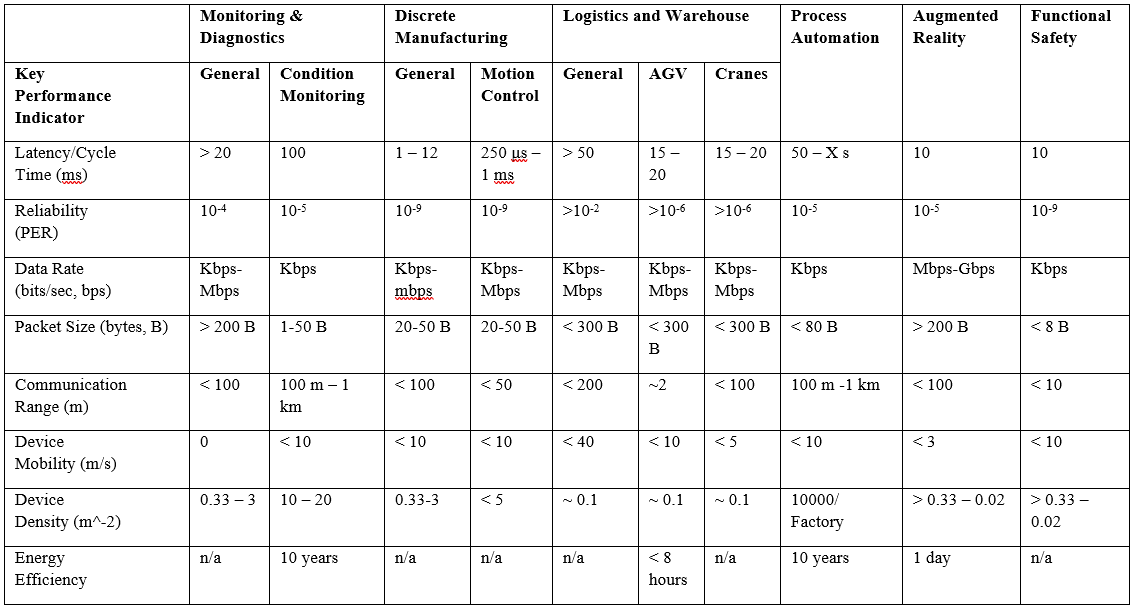
\includegraphics[width=\textwidth]{chapter-soa/etsi-reqts}
\end{table}

\subsection{An Industry Requirements Perspective}\label{sec:litreview:industry}

% Table generated by Excel2LaTeX from sheet 'FromKarl2019'
\begin{table}[!tb]
	\centering
	\caption{An Industry Requirements Perspective of Different Industrial Communication Scenarios as presented in~\cite{Luvisotto2017}.}
	\label{soa:industry-reqts-persp}%
	
% Table generated by Excel2LaTeX from sheet 'Industry'
\begin{tabular}{|p{7.5em}|p{4.215em}|p{4.215em}|p{4.215em}|p{4.215em}|}
	\toprule
	\textbf{Scenario} & \textbf{\# of nodes} & \textbf{Update rate, Hz} & \textbf{Goodput, bps} & \textbf{System range, m} \\
	\midrule
	Building Automation & $10^{2}-10^{3}$ & $10^{-1}$ & $10^{3}-10^{4}$ & 10-100 \\
	\midrule
	Process Automation & $10^{2}-10^{3}$ & \multicolumn{1}{l|}{10} & $10^{5}-10^{6}$ & 10-100 \\
	\midrule
	Factory Automation & $10^{2}-10^{3}$ & $10^{3}$ & $10^{7}-10^{8}$ & 10-100 \\
	\midrule
	Power Systems Automation & $10^{1}-10^{2}$ & $10^{4}$ & $10^{7}-10^{8}$ & $10^{2}-10^{3}$ \\
	\midrule
	Power Electronics Control & $10^{2}-10^{3}$ & $10^{5}$ & $10^{9}-10^{10}$ & 10-100 \\
	\bottomrule
\end{tabular}%

	
\end{table}%

Another industry perspective presented in~\cite{Luvisotto2017}, targeted ultra-high-performance wireless for various scenarios ranging from building automation to the switching of power electronics equipment. An example of system-level requirements for different industrial communication scenarios is captured in Table~\ref{soa:industry-reqts-persp}. The scenario Building Automation consists of all control operations performed within buildings, such as lighting, heating, surveillance, energy management, etc. Process Automation is involved in chemical, mining, oil, and metallurgic processes. \textit{Factory Automation} is a general term referring to the factory production line, such as assembly and packaging. More demanding scenarios include \textit{Power Systems Automation} in which control for power distribution is performed. \textit{Power Electronics Control} focuses on the synchronized control of power electronic devices. All these scenarios have distinct requirements. Luvisotto states that for a wireless high performance system, a \gls{per} of $10^{-9}$ is perceived as tolerable~\cite{Luvisotto2017}. It is important to clarify this PER is at the application layer and it is possible to have a high PER at the physical layer and still achieve $10^{-8}$ at the application layer with transmission and information redundancy. It is proposed that a latency requirement of $10{\mu}s$ is required for power electronics applications. It is stated that \textit{Factory Automation}, \textit{Power Systems Automation}, and \textit{Power Electronics Control} are the scenarios where their particular technology is applicable. The power electronics industry is very distinctive in the difficulty in meeting their challenges requirements; however, these requirements are not typical of all industry scenarios.

\subsubsection{NIST Validated Requirements Perspective}\label{sec:litreview:nist}

% Table generated by Excel2LaTeX from sheet 'FromKarl2019'
\begin{table}[!tb]
	\centering
	\caption{\gls{nist} Wireless Requirements Perspective as presented in~\cite{Montgomery2019}.}
	\label{soa:nist-reqts-persp}%
	
	% Table genera% Table generated by Excel2LaTeX from sheet 'FromKarl2019'
	\begin{tabular}{|p{5.715em}|p{4.855em}|l|l|l|l|l|}
		\toprule
		\multicolumn{2}{|p{10.57em}|}{\textbf{User Requirement}} & \multicolumn{1}{p{4.355em}|}{\textbf{Class 0:}} & \multicolumn{1}{p{4.355em}|}{\textbf{Class 1:}} & \multicolumn{1}{p{4.355em}|}{\textbf{Class 2:}} & \multicolumn{1}{p{4.355em}|}{\textbf{Class 3:}} & \multicolumn{1}{p{4.355em}|}{\textbf{Class 4:}} \\
		\midrule
		\multirow{2}[4]{*}{Latency (ms)} & Typical & 4     & 4     & 20    & 4     & 50 \\
		\cmidrule{2-7}\multicolumn{1}{|l|}{} & Minimum & 0.5   & 0.25  & 4     & 0.5   & 4 \\
		\midrule
		Reliability & Typical & \multicolumn{1}{p{4.355em}|}{$10^{-7}$} & \multicolumn{1}{p{4.355em}|}{$10^{-7}$} & \multicolumn{1}{p{4.355em}|}{$10^{-7}$} & \multicolumn{1}{p{4.355em}|}{$10^{-7}$} & \multicolumn{1}{p{4.355em}|}{$10^{-6}$} \\
		\cmidrule{2-7}(Pr. Loss) & Minimum & \multicolumn{1}{p{4.355em}|}{$10^{-7}$} & \multicolumn{1}{p{4.355em}|}{$10^{-7}$} & \multicolumn{1}{p{4.355em}|}{$10^{-7}$} & \multicolumn{1}{p{4.355em}|}{$10^{-7}$} & \multicolumn{1}{p{4.355em}|}{$10^{-7}$} \\
		\midrule
		Scale & Typical & 8     & 10    & 10    & 1     & 100 \\
		\cmidrule{2-7}(\# of links) & Maximum & 16    & 30    & 30    & 4     & 300 \\
		\midrule
		\multirow{2}[4]{*}{Range (m)} & Typical & 10    & 10    & 10    & 10    & 10 \\
		\cmidrule{2-7}\multicolumn{1}{|l|}{} & Maximum & 30    & 30    & 30    & 30    & 30 \\
		\midrule
		\multirow{2}[4]{*}{Payload (B)} & Minimum & 6     & 8     & 8     & 8     & 12 \\
		\cmidrule{2-7}\multicolumn{1}{|l|}{} & Maximum  & 24    & 1024  & 1024  & 1024  & 33000 \\
		\midrule
		Update Rate & Typical & 125   & 125   & 25    & 125   & 10 \\
		\cmidrule{2-7}(Hz)  & Maximum & 1000  & 2000  & 125   & 1000  & 125 \\
		\bottomrule
	\end{tabular}%
\end{table}%

Using requirements from standardization bodies such as \gls{isa}~\cite{ISATR100-2011}, \gls{etsi}~\cite{etsi103588}, and industry, a distilled and validated set of requirements is produced in Table~\ref{soa:nist-reqts-persp}. The same \gls{isa} class-labeling scheme from Table 1 has been adopted to categorize applications. The \gls{isa} classification scheme groups applications according to mission-criticality. Class 5 is not included in Table 6 because the requirements were not adequately supported by existing wireless standards. It is believed that existing wireless standards do not jointly meet the requirements for all the industrial use case classes presented; however, the design of new wireless technology that applies to industry can be accomplished using the requirements in Table 6. The authors based the user requirements, shown in Table~\ref{soa:nist-reqts-persp}, on what is believed to be necessary for effective and realizable communications within factory workcells. Latency and reliability are fundamental requirements for time-sensitive applications. Latency and reliability can often be considered jointly as information that is delayed beyond a time threshold may be considered as lost information. Scale is important to enable large enough capacity for a network, while maintaining latency and reliability targets. Range provides a maximum expected distance between linked nodes before the network can no longer guarantee performance of the \gls{iwn}. These requirements were developed based on the philosophy of avoiding excessive and unreasonable performance expectations on the wireless systems. For instance, requiring a range of 100 meters for a workcell device that only needs to operate within 10 meters would be unreasonably strict and would be considered overkill for many applications where shorter range would be sufficient and more practical. Justification for requirements is provided in~\cite{Montgomery2019}.



\section{Systems Modeling}\label{chapter:soa:modeling}

Systems modeling is the process of developing abstract representations of a system to analyze its features, strengths, and weaknesses, or to communicate its design.  Systems models are uniquely useful when a system is large or complex, and the interactions of among components within the system are unknown or difficult to understand.  With \glspl{cps} in which the behavior of a physical system is strongly tied to the behavior of a computing or communication system, systems modeling is useful in identifying components and understanding cyber-physical links and data flows.   This chapter provides a background to the reader in the state of the art in systems modeling.  Particular attention is given on the research done to how modeling tools and techniques are applied to the problem of the wireless smart manufacturing workcell, the components of such a workcell, or the data flows within the workcell.  The \gls{sysml} model was developed to formalize and identify key components, interfaces, and constraints of the factory workcell.  The model developed is intended to include elements of both the physical system and network controlling behavior.  Therefore, the state of the art explored focuses on research performed to model both domains simultaneously capturing architecture and behavior.  The exploration of the literature is divided into two components: 1) modeling languages in general, and 2) the use of \gls{sysml} in modeling systems.

\subsection{Modeling Languages} \label{sysml:sec:languages}

Current modeling work on factory workcells is mainly aimed at defining and characterizing the subsystems, such as human staff, robots, and machine tools, in individual applications. By following blueprints (schematics) of production tasks, the work flow can be divided into separate assignments which are distributed by a task dispatch system to individual machines~\cite{IkeaBot}. Analytical models are thus obtained for performance analysis in workcells. As an example, a mathematical model for real-time performance analysis of a gantry workcell with robots is established with the timing and the randomness of tasks and disruptions are captured in~\cite{8098604}. In \cite{Ou2017}, the same model is used to investigate the natural system properties such the system cycle and waiting times and to identify bottlenecks through studying the sensitivity of each machine. Similarly, the steady state analysis for production lines with uncertainties is performed through various decomposition methods~\cite{Colledani2013,doi:10.1080/00207543.2012.713137,doi:10.1080/00207540500385980}. In \cite{Colledani2013}, a decomposition method is presented for the analysis of continuous flow lines. The presented model is used to analyze flow lines with single and multiple failure mode machines and machines subject to aging and having up and down times.  This work in particular was useful in the application of models to process control applications. In \cite{doi:10.1080/00207543.2012.713137}, a model to evaluate the performance of transfer lines with unreliable machines and finite transfer-delay buffers is presented. A decomposition method is introduced to model the transfer line, using the general-exponential distributions instead of the exponential distributions to approximate the repair time distributions of the fictitious machines. In \cite{doi:10.1080/00207540500385980}, the authors present a model for evaluating the production rate and distribution of inventory of a closed-loop manufacturing system with unreliable machines and finite buffers. The model accounts for the different sets of machines that could cause blockage or starvation to other machines. In \cite{QChang,Liu2012}, the performance analysis modeling for serial production lines with disruptions is explored by studying the impact of each individual downtime event in terms of permanent production loss and financial cost. These analytical models generally work well for simple systems with small number of components or few interactions between various equipment. Also, the analytical models can be used to abstract industrial systems to understand various performance trends without studying various details. As a result, a comprehensive model that include network and production impacts on the industrial workcell is introduced.  

Furthermore, the reconfigurable workcell architecture is widely considered for automated manufacturing. The main advantage of reconfigurable workcells lies in the flexibility of reconfiguration of workcell components to adapt to varying production requirements where the assembly of the work cell is optimized for each specific task~\cite{Chen2001.rapid}. In the workcell that hosts robots, robots are installed therein to allow for autonomous configuration within their workspace \cite{Gaspar2017,Molina2017,Ferreira2011}. Approaches and performance criteria for reconfigurable robotic systems have recent developments in control architectures to achieve various levels of reconfigurability \cite{Fulea}. The \gls{nist} has defined a \gls{not} model which can depict the structure of workcells by a group of NoT building blocks and model the behaviors of individual components in a workcell~\cite{NIST800-183}.  The NIST NoT model is focused primarily on sensor networks and the collection of data rather than the collection and then subsequent action on data.  Actuation is cursorily noted, and, as such, cross-domain interactions between the physical system and the network are not addressed. Several other robotic workcell architectures are discussed in the literature. In \cite{OpenArch}, a reference model for a control system functional architecture applied to open architecture robot controllers is presented. In \cite{Carpanzano2007}, a methodology to develop self-adaptive factory automation solutions is illustrated, using a novel modular simulation-based method. With the increase in complexity and reconfigurability of workcells, studying various production criteria and network impacts requires introducing new models to capture these interactions and requires sufficient abstraction to model different configurations and scenarios of industrial work-cells.  

In a workcell model, data flows are used to capture the trajectory of system information exchange between workcell components and identify their roles in specific operations~\cite{OpenArch}. For example, safety-related operations may employ vision systems and various proximity sensors that generate proximity data and transmit them to the safety manager to define safety zones in an automotive assembly work-cell~\cite{safeeye}. 
In another example, data flows are enabled in a workcell to capture human operator gestures from embedded cameras in human-robot collaborations~\cite{cobotcell}. These gestures can be later regenerated in simulators based on the transmitted position data from the field to optimize workcell safety operations~\cite{Duan2009}. Currently, most of the workcell information in these scenarios are transmitted by wired networks. Wireless networks have gained increasing attention to enable data flows in the highly connected workcells. Wireless standard bodies have proposed their network reference models in factory environments which include the workcell cases in the data-centric architecture~\cite{ETSI889, KPItable}. In these models, individual workcells are treated as a subnetwork of field instruments attached with data aggregations that manage network connections and transfer data traffic to edge and cloud servers in various applications. Wireless connections are featured with flexible network topology to agree with a variety of transmission needs, especially in reconfigurable workcells. Meanwhile, data traffic flows are characterized by select performance metrics, such as transmission latency and link reliability, to categorize industrial use cases~\cite{KPItable}. 

Current modeling efforts set the boundaries of their systems of study at the edge devices without further discussions on the impact of wireless performance on the operations of industrial systems. For example, the abstracted disruptions in \cite{QChang,Liu2012} that cause plant down-times may include wireless network impacts which are not yet distinguishable with specific characteristics of wireless networks. As indicated by the earlier empirical studies~\cite{Liu2016}, such physical systems may have different responses to network performance which will vary with the operational configuration such as the served application and the deployed control algorithms. 

Therefore, much research has been done in the area of modeling of complex systems; however, an opportunity exists for exploring applying systems modeling to the industrial workcell.  In particular, those workcells that have strong network interactions have been left unstudied.  It is also necessary to incorporate the features of wireless communications networks into the modeling architecture of physical workcells such that cross-domain interactions between the physical system and the network may be studied.  

\subsection{Systems Modeling Using SysML} \label{sysml:sec:systemsmodeling}

The primary goal of modeling a system is to capture knowledge of a process in a simplified way~\cite{SysModel2004}. A secondary goal of a system model is to provide a level of abstraction that may allow for the discovery of new knowledge such as how two systems will interact. There are multiple ways of designing and presenting system models. Well-behaved systems can be represented by a system of equations using mathematical tools~\cite{SimModel1999}. Such models provide excellent constraint definition, but equations alone lack the semantics to describe architecture and detailed information flow of a realizable system.

Moreover, by deploying functional block diagrams, major functional components and flow of information or material are captured. As shown in Fig.~\ref{sysml:fig:fbd-system}, a physical process interacts with a control system through a wireless network.  Measured values, $Y$, from sensors flow to the controller through a wireless network and arrive at the controller delayed and modified, $\bar{Y}$. Similarly, commands, $U$, flows from the controller to the actuators through the wireless network. Such diagrams may be used to model feedback control systems in which the origination and routing of information are immaterial for study. However, the architecture and interfaces remain at a very high level of abstraction making analysis difficult. In such cases, delay and loss using such tools are often modeled stochastically. Using architectural diagrams helps identify components, interfaces, and information flow. For factory systems, architectural block diagrams are often manifested as schematics. However, such diagrams have their own limits in industrial practices. On one hand, they lack the semantics necessary to describe the constraints that formal equations and functional block diagrams offer. Meanwhile, they also lack the capability of capturing behaviors or complex interactions between the physical system and the information infrastructure such as a wireless network. 

\begin{figure}
	\centering
	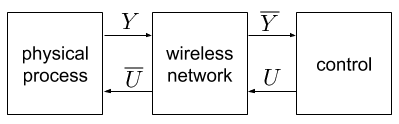
\includegraphics[width=0.65\columnwidth]{./chapter-sysml/diagrams/fbd-system}
	\caption{Functional block diagram of a \gls{cps} in which a physical process and an automation system interact through a wireless network.  In a \gls{cps}, the automation/control system acts using estimated and/or delayed versions of the process variables, whereas, the physical process uses estimated and/or delayed versions of commands from the controller.}
	\label{sysml:fig:fbd-system}
\end{figure}

An alternative to schematic diagrams is \gls{sysml}~\cite{SysML2017}. SysML is a general purpose modeling language that is often used for \gls{mbse} practice within industrial systems~\cite{MBSEandSysML}. SysML provides structural, behavioral, and parametric semantics for the analysis of complex systems. For examples, systems analysis using SysML enables capturing and communicating system requirements and design which include hardware, software, firmware, information flows, and processes with graphical notations. Within the factory automation industry, engineers are adopting SysML in the form of MBSE to develop realizable operational models of the factory and data flow processes. MBSE models address verification of design through executable simulations depending on the modeling tool.  The SysML specification is defined in~\cite{SysML2017}.  In SysML, the basic semantic constructs of the language are Packages, Blocks, Ports, Interfaces, and Constraints, in addition to the constructs provided by the \gls{uml}. Packages are logical grouping of model elements. Package relationships are captured using the \gls{pkg}. Relationships of these constructs are captured in the \gls{bdd}.  The internal composition and connectivity of parts are captured in the \gls{ibd}. SysML includes other types of diagrams and semantic constructs that are not required for this analysis and are not explained here. The SysML modeling language is comprehensive; however, the size and number of diagrams within the model are too extensive to include here in this thesis.  Therefore, the reader is encouraged to explore the SysML model defined in~\cite{Candell2018SysML.JRES}.  A useful primer on SysML may be found in~\cite{Friedenthal2015.SysML}. 

Examples of the use cases and methodologies of using different graphical models for the analysis of manufacturing systems are explored in~\cite{Lutjen2015.GramosaMethod,Luder2011.GraphicalModeling,Jia2013.GraphicalModeling,Alvarez2013.GraphicalModeling}.  In~\cite{Quinsat2017.SysML}, SysML is used to capture both composition and behavior of an additive manufacturing workcell.  A survey of applying graphical modeling languages in capturing information flows within a product service system which may be applied to manufacturing enterprises~\cite{Durugbo2011.GraphicalModeling}.  This approach compliments these previous examples by combining the operational and wireless information transport systems together in a single model, thereby facilitating a single model that may be used for simulation and other systems engineering analyses.  While various architectures for the workcell exist as exemplified in the literature, a common language and framework for communicating architecture and information flow has not been established for cross-domain interactions between the manufacturing system and its supporting communication networks.  

\Gls{sysml} contains the semantics for such engineering capture and provides an industry accepted language for communicating composition, interfaces, and information flow. Moreover, SysML provides the semantics for assigning properties to any model element such that those properties are made  available for analysis using other tools such as Prot\'eg\'e \cite{StanfordUniversity.Protege} and the \gls{owl} \cite{W3C2012.OWL}.
It is important to understand that while \gls{sysml} provides semantics for a formal capture of architecture, information flow, and parametric constraints, it may also be used for a higher-degree of abstraction provided by the functional block diagrams.  

\section{Use of Databases for Performance Analysis}
\Glspl{gdb} were employed within this thesis to better organize the copious amounts of experimental data resulting from experiments run within the industrial wireless testbed.  Therefore, an investigation into the application of data management approaches was conducted.  This investigation included the application of \glspl{gdb} for the problem of data curation and organziation of large amounts of network and physical systems performance data that had correlation between events occurring in time.

The \gls{gdb} is a class of the \gls{nosql} database.  The \gls{nosql} database is a non-relational database in which the structure data is not predetermined and cannot be onforced by the database.  Due to its advantages including scalability, efficiency, and flexibility, \gls{nosql} databases are a popular alternative to relational databases in the case of large amounts of data in various applications~\cite{doi:10.1108/17440081311316398}. The \gls{gdb} is a kind of \gls{nosql} database approach that additionally handles complex relationships~\cite{8123475}. \Glspl{gdb} are widely adopted in various industry-related applications and use cases such as network operations, fraud detection, and asset and data management~\cite{top5}. Relationships in social networks have been modeled using a \gls{gdb} for structural information mining and marketing~\cite{Gomez-Rodriguez:2012:IND:2086737.2086741}. On the other hand, business solutions for scenarios with multiple large data sources require distributed processing in decision making for various problems such as fraud detection, trend prediction, and product recommendation~\cite{Skhiri2013}.

Multiple surveys regarding \glspl{gdb} are presented to describe the associated models, tools, and their features in~\cite{Angles:2008:SGD:1322432.1322433,7148480,GDB_overview}. In~\cite{Angles:2008:SGD:1322432.1322433} the graph database is introduced as a technology that experienced as many technologies do, some hype, and early death, and then a later resurrection.  Graph databases have recently regained some interest in industrial and cyber-physical research because of the amount of data resulting from big-data and the \gls{iot}/\gls{iiot}.  Data in which graph-like qualities exist are presented as candidates for use by the database technology.  In ~\cite{GDB_overview}, a performance study is performed to make the case for using graph databases to enhance query speed for interconnected data.  The study showed a strong preference for using graph databases in place of the relational database.  The performance of different GDB tools and methodologies is analyzed and compared in~\cite{Jadhav2015ComparativeAO,Macko:2013:PIG:2485732.2485750}. Multiple comparisons in these articles have shown improved performance of Neo4j in the general features for data storing and querying, and data modeling features such as data structures, query languages and integrity constraints.  

Examples of applications and implementations of \glspl{gdb} are presented in~\cite{modern_models} to show their use on enterprise data, social networks, and determining security and access rights. It was found that GDBs provide the much needed structure for storing data and incorporating a dynamic schema. On the other hand, query languages are used to extract data including traversing the database, comparing nodes properties, and subgraph matching~\cite{Wood2012QueryLF}. While \gls{gdb} are of particular interest in traversing and querying interconnected dataset found within social networks, it is proposed that data resulting from \glspl{cps} is not entirely similar, and therefore, use of the graph database for analyzing performance measurement data from the factory workcell is explored. 

Furthermore, industrial data analytics play an essential role in achieving the smart factory vision and improving decision-making in various industrial applications. Five main industrial data methodologies are generally studied including highly distributed data ingestion, data repository, large-scale data management, data analytics, and data governance~\cite{DBLP:journals/corr/abs-1807-01016}. Industrial data processing offers valuable information about various sections of industrial applications including inefficiencies in industrial processes, costly failures and down-times, and effective maintenance decisions~\cite{JLee-BigData, Raptis2019}.  The methods of industrial data analytics can be split into different categories such as descriptive, diagnostic, predictive, and prescriptive analytics~\cite{Dai2019}. Descriptive and diagnostic analytics are responsible for analyzing historic data and the causes of events and behaviors. Predictive and prescriptive analytics require more processing power, anticipate the trends of data, and deploy the historical data in making decisions to achieve production goals. Examples of industrial data analytics frameworks are found in~\cite{GEBigData2019, Wan2017, Courtney2019, ABBBigData2019}. In~\cite{GEBigData2019}, a platform for performing industrial big data analysis is presented where the performance requirements are introduced to achieve a cost-effective operation. In~\cite{Prevent_7857790}, a manufacturing big data solution for active preventive maintenance in manufacturing environments is proposed. Various other frameworks for industrial data analysis can be found, where the importance of using data analysis in decision making is emphasized.

Due to their advantages including scalability, efficiency, and flexibility, \gls{nosql} databases are a popular alternative to relational databases in the case of large amounts of data in various applications~\cite{doi:10.1108/17440081311316398}. The \gls{gdb} is one kind of \gls{nosql} database approaches that additionally handles complex relationships~\cite{8123475}. GDBs are widely adopted in various industry-related applications and use cases such as network operations, fraud detection, and asset and data management~\cite{top5}. In~\cite{8721634}, authors have proposed  a new object tracking approach for surveillance applications. The GDB approach is selected to contribute to the scalability of the proposed scheme and support the required connectivity analysis for the object tracking. Moreover, relationships in social networks have been modeled using a GDB for structural information mining and marketing~\cite{Gomez-Rodriguez:2012:IND:2086737.2086741}. On the other hand, GDBs are also deployed in business solutions for scenarios with multiple large data sources which require distributed processing in decision making for various problems such as fraud detection, trend prediction, and product recommendation~\cite{Skhiri2013}. 


%Industrial data analytics play an essential role in achieving the smart factory vision and improving decision-making in various industrial applications. Five main industrial data methodologies are studied including highly distributed data ingestion, data repository, large-scale data management, data analytics, and data governance~\cite{DBLP:journals/corr/abs-1807-01016}. Industrial data processing offers valuable information about various sections of industrial applications including inefficiencies in industrial processes, costly failures and down-times, and effective maintenance decisions~\cite{JLee}. In~\cite{GEBigData2019}, a platform for performing industrial big data analysis is presented where the performance requirements are introduced to achieve a cost-effective operation. Various other frameworks for industrial data analysis can be found in~\cite{Courtney2019,ABBBigData2019}, where the importance of using data analysis in decision making is emphasized.


\section{Machine Learning in Performance Estimation}\label{chapter:soa:ml}

In the literature, two types of interference signals are considered, namely, intentional or unintentional interference. Methods to estimate, avoid, or mitigate interference are required for the deployment of reliable and deterministic IWSs. Machine learning has been widely used to detect and estimate interference information to enhance the performance of interference management algorithms.  Machine was investigated and applied to the problem of inferring wireless link quality from observations of the physical system without expensive, highly complex spectrum analysis tools.  Furthermore, factory technicians are typically not trained in wireless interference estimation or radio engineering.  A need to assess performance of the wireless network within factories is needed; however the cost of radio equipment stationed within the factory workcell can be cost-prohibitive and detrimental to the adoption of wireless technology within the factory.  Therefore, machine learning, e.g., artificial intelligence, can be a valuable tool.  In this chapter, the state of machine learning application to wireless performance estimation is presented.

The interference analysis in \glspl{cps} is considered in multiple works for various scenarios. In~\cite{8639006}, in-network interference mitigation techniques are discussed for ultra reliable low-latency wireless communications systems. The work focuses on mutual interference mitigation in an industrial automation setting, where multiple transmissions from controllers to actuators interfere with each other. In \cite{Kumar2019}, an interference mitigating receiver architecture is proposed. The application scenarios are smart homes and modern factories where dense wireless communications devices exist. Moreover, in~\cite{Bhushan2014.NetworkDesensUsingIntfCancellation}, interference cancellation of transmissions from neighboring cells in a \gls{5g} cellular network is presented. In~\cite{Gomes2017.LQEinWSNs}, a method using a dedicated node for \gls{lqe}  obtained through received data packets to identify interference and multi-path without introducing additional traffic is presented. In~\cite{Baccour2012.SurveyOnLinkEstimation}, a taxonomy of channel link quality techniques is presented providing a valuable survey on LQE algorithms and asserting the importance of \gls{lqe} in IWSs. In~\cite{Frounhoffer.Troubleshooting}, failure analysis and wireless network troubleshooting are performed whenever the \gls{cps} is not functioning properly. Interference analysis is one major part of the troubleshooting procedure which is performed through traffic patterns and wireless spectrum analysis. Also, in~\cite{NIST.InterfCoexCritical}, the use of spectrum analysis for interference detection and estimation is proposed for IWSs. 

On the other hand, intended interference (i.e., jamming) can lead to service denial or poor performance in wireless networks. In~\cite{8631535}, a literature review is presented which includes an overview of recent research efforts on networked control systems under denial-of-service attacks such as jamming attacks in wireless channels. One of the discussed challenges is how to achieve ultra-reliable low-latency "signalling" within industrial applications. In~\cite{Cetinkaya_2019}, a discussion is also provided on the recent developments concerning the design of attack-resilient control and communication protocols. Generally, a jamming attacker can block transmission of packets by emitting strong interference signals to a wireless channel \cite{1637931,5473884}. Jamming attacks can target various wireless technologies and hence can become a major concern for control systems, since they are easy to launch \cite{5473884}. It is shown in \cite{10.1007/978-3-319-07788-8_40} that off-the-shelf hardware can be used for generating jamming attacks on wireless networks. In cases of physical-layer attacks, the jamming attacker targets a frequency band and is not required to follow the wireless protocol where it can cause a decrease in the SIR thus preventing the receiver from successfully detecting transmitted packets \cite{10.1007/978-3-319-07788-8_40}. In the case of \gls{mac}-layer attacks, both the packet sender and the jamming attacker operate on the same channel; the jamming attacker’s goal is to cause packet collisions.

In~\cite{8726803}, the authors evaluate the \gls{cps} resilience to jamming attacks that disrupt wireless communications. They considered three jamming strategies which are the constant, random, and protocol-aware jamming. They showed through experimental results that various \gls{cps} control schemes are susceptible to constant and random jamming while the time-triggered control schemes are susceptible to protocol-aware jamming. Moreover, resilience of \glspl{cps} is also considered in~\cite{6425868,DEPERSIS2014134,7402971,7575630} where periodic jamming is considered in \cite{6425868} while the jamming strategy in~\cite{DEPERSIS2014134,7402971,7575630} is unknown. 

Machine learning has been used for detection and estimation of jamming attacks. In~\cite{Chen2019}, an unsupervised machine learning algorithm based on a multi-layer auto-encoder is used to extract the interference source spectrum features. These features are then used to distinguish interference sources type and location without labeling measured data. In~\cite{7911887},  an unsupervised approach using a recurrent neural network is used to detect anomalies in the \gls{cps} performance and identify attacked sensors. In~\cite{Junejo2016DataDP}, a behavior based machine learning intrusion detection approach  is proposed to detect attacks at the physical process layer. The results are validated through experimental study of a real modern water treatment facility. In~\cite{Beaver:2013:EML:2584691.2584722}, the viability of machine learning methods in detecting the new threat scenarios of command and data injection is assessed. In that work, command and control communications in a critical infrastructure setting are monitored and vetted against examples of benign and malicious command traffic to identify potential attack events. In~\cite{6900095}, the authors assess discriminating types of power system disturbances through machine learning by detecting jamming attacks. They evaluate various machine learning methods as disturbance discriminators and discuss the practical implications for deploying machine learning systems as an enhancement to existing power system architectures.

Therefore, in the literature, it is shown that \gls{lqe} through direct observation is one important but insufficient aspect of assessing the impact of link quality on a \gls{cps}. It is asserted that by jointly observing the performance of the physical and wireless components of a CPS, the complete perspective of the quality of the wireless link and its impact on physical performance can be obtained. Since interference is such an important topic in the wireless CPS, a novel method is proposed in~\cite{Candell_ISIT_2019,Candell2020.Jrnl.ISATrans} presented in Chapter~\ref{chapter:ftml} in which a learning network simultaneously (1) makes observations of the physical system using ground truth measurements, and (2) infers the quality of the wireless communication system in terms of SIR using an experimental model of a relevant use case found in industry.




\part{Thesis Contributions}\label{part:techical}



\newcommand{\argmax}{\operatornamewithlimits{arg\ max}}
\newtheorem{theorem}{Theorem}[section]
\newtheorem{lemma}[theorem]{Lemma}
\newtheorem{property}[theorem]{Property}

\chapter{Survey: Industrial Wireless Technology}\label{chapter:reswk}

% Some very useful LaTeX packages include:
% (uncomment the ones you want to load)
	
\chapterintro*

The use of wireless technologies within factories demands a comprehensive understanding of the problems and potential solutions associated with the rigors of the manufacturing environment. A clearly defined problem space would significantly ease the selection and deployment of appropriate wireless solutions to connected factory systems.  A mapping of potential technologies to classes of use cases within the problem space will be useful to factory operators, system integrators, and wireless systems manufacturers.  Identification of use cases, not addressed by existing technologies, may be used to spur targeted innovation where reliability, resilience, latency, and scalability are joint concerns. Motivated by the industry need for independent practical guidelines and solutions to difficult wireless control problems, this paper provides a classification of the problem categories where networking technologies may be deployed. It then maps specific technologies that may serve as interim or terminal solutions for those use cases identified within the problem space taxonomy. This chapter is intended to provide a detailed exposition of the requirements directed towards industrial wireless.  It draws on various sources of requirements captured by academic literature, industry organizations, and standards institutes.  The work therefore presents a picture of the requirements landscape at the beginning of this research.  Further work in this area can be found in~\cite{Montgomery2019} and~\cite{Raptis2019}.

	\section{Introduction} \label{sec:intro}
    \subsection{Purpose}
    Industrial wireless is a key enabling technology for the Industrial Internet of Things (IIoT).  The IIoT promises lower costs of deployment, increased mobility of factory assets, massive interconnectivity, improved situational awareness, increased efficiency of the operation, and improved operations analytics.  IIoT and advanced manufacturing technology seek to improve competitiveness, productivity, and responsiveness to customer needs. However, it is often stated that where wireless is deployed, factory enhancements fail to meet expectations typically in areas of reliability, resilience, and scalability. Moreover, transmission security is often cited as an area of concern. Risk averse organizations will establish policies that preclude wireless to be deployed for specific types of applications such as feedback control or safety. Yet, factory operators are increasingly demanding that wireless be deployed for critical and sometimes perceivably dangerous applications.  For this reason, the
\iftoggle{blindcopy}{(BLIND COPY - NAME REMOVED)}{National Institute of Standards and Technology (NIST)} 
is developing best practice guidelines to help factory operators select appropriate wireless systems for their particular use case and then deploy that solution effectively.  Such a mission requires participation by factory operators, system integrators, and device manufacturers. A comprehensive taxonomy of the existing problem space within industry and a survey of existing and missing technologies are necessary to the success of such a mission. This paper provides the author's classification of industrial wireless cases and links current technologies to those use cases if applicable. 
    
%    \subsection{Related Work}
%    %Mohamed will provide.  High level mentions and limitation.  Stop.
%The use of industrial wireless networks has been studied in many works in the literature. However, no comprehensive survey of the whole problem space of industrial communications has been performed.
%
%In \cite{6248648}, the authors have introduced a comparison between the commercial and industrial communications networks where an industrial network has been divided to five different levels. These levels include field equipment, controller level, application, supervisory, and external networks. The differences in requirements between different levels are discussed. Moreover, three types of information are considered which are control, diagnostic, and safety information as described in \cite{4118467}. However all these levels of industrial networks are mentioned in \cite{6248648}, the article focuses only on the manufacturing and instrumentation communications and does not consider other types of communications networks that exist in industrial environments. Also, in \cite{What}, three levels of communications are considered which are device, control, and information levels. Moreover, the current wired industrial technologies for these levels are discussed briefly.
%
%More works focused on the communications at the field devices level where sensing and control information is transfered. In \cite{7005074},  the communication between field devices has been studied where the requirements for a large number of nodes may not be achieved. The use of fieldbus solutions limit the scalability and resilience and hence industrial Ethernet capabilities are introduced in this article. Moreover, in \cite{Connectivity}, the communication for monitoring and control operations is discussed. A comparison between fieldbus technologies, industrial Ethernet, and wireless solutions is performed. The author has discussed the use of Wi-Fi, Bluetooth, ZigBee, and WirelessHART technologies in industrial applications. Similarly, the authors of \cite{6490786} considered the industrial communications networks requirements in process automation specifically at field devices level. Finally, in \cite{GE_Professional}, many case-studies are discussed for communication networks in industrial scenarios. Moreover, the design steps for these solutions are briefly discussed.

    \subsection{Paper Organization}
    The rest of the paper is organized as follows. The problem space for employing wireless networks is presented in Section II. Then, the technical considerations while designing industrial wireless networks are discussed briefly in Section III.  In Section IV, a mapping between the problem space and the current technology space is provided. Finally in Section V, future directions and conclusions are presented.
    
    \section{Problem Space}
    
    \subsection{Introduction and Success Considerations}
    Implementing a factory enhancement program requires economic and technical planning, and justification.  Wireless technologies by themselves are interesting and can provide value; however, it is incumbent upon plant leadership to fully assess the potential risks and benefits of the enhancement before proceeding with deployment. Wireless technologies are often deployed as a means to monitor or control factory process. They have the potential to unlock improved observability and control. By understanding the problem space and the risks and benefits of potential wireless solutions, factory operators can assess if the rewards outweigh the risks.  In navigating the risk/reward question, it is asserted that any wireless program must address one or more of the following success criteria before embarking on an enhancement involving wireless communications.  These criteria are defined as follows:
    
	\paragraph{Reliability} Wireless systems can be deployed to add redundancy or replace faulty wired solutions with a more reliable wireless solution for particularly harsh industrial environments where temperature, pressure, vibration, radiation, and chemistry may make wired communication unreliable.
	\paragraph{Safety} Wireless systems may be used to detect or prevent injury to humans.  They may be used as backup to wired systems or serve as the primary communication system.
	\paragraph{Production Cost} Wireless systems can increase observability and the resulting data may be used for precise optimization of the factory operations, machine scheduling, and maintenance.
	\paragraph{Quality} Various measurements are possible to improve quality of the factory output. Using wireless solutions may make deployment of sensors and inspection equipment more practical. 
	\paragraph{Environment} Wireless sensors and control mechanisms may be used to detect toxic conditions and prevent environmental accidents from occurring.  Wireless actuation devices may serve to improve reliability and address environmental mitigation control. 
	\paragraph{Regulations} In some scenarios, government regulations may require specific sensor instrumentation to be deployed for certain scenarios.  Wireless solutions could make regulatory compliance practical or cost effective in some cases.
      
    \subsection{Use Cases}
    
    Once a plant upgrade enhancement program is initiated, and some type of wireless technology is anticipated, the first step in realizing the program is defining and understanding the problem space where wireless technologies will be used. To support this assessment, a taxonomy of industrial use cases to which wireless communication may be employed is given.  The industrial wireless landscape is diverse, and a classification of those technologies can be helpful in mapping particular technologies to an application.  The author's classification is shown in Fig.~\ref{fig:problemspace} and includes instrumentation, safety, and back-haul connectivity, among others. Each class of the problem space is explained in the following subsections.  

\begin{figure}[t]
\centering
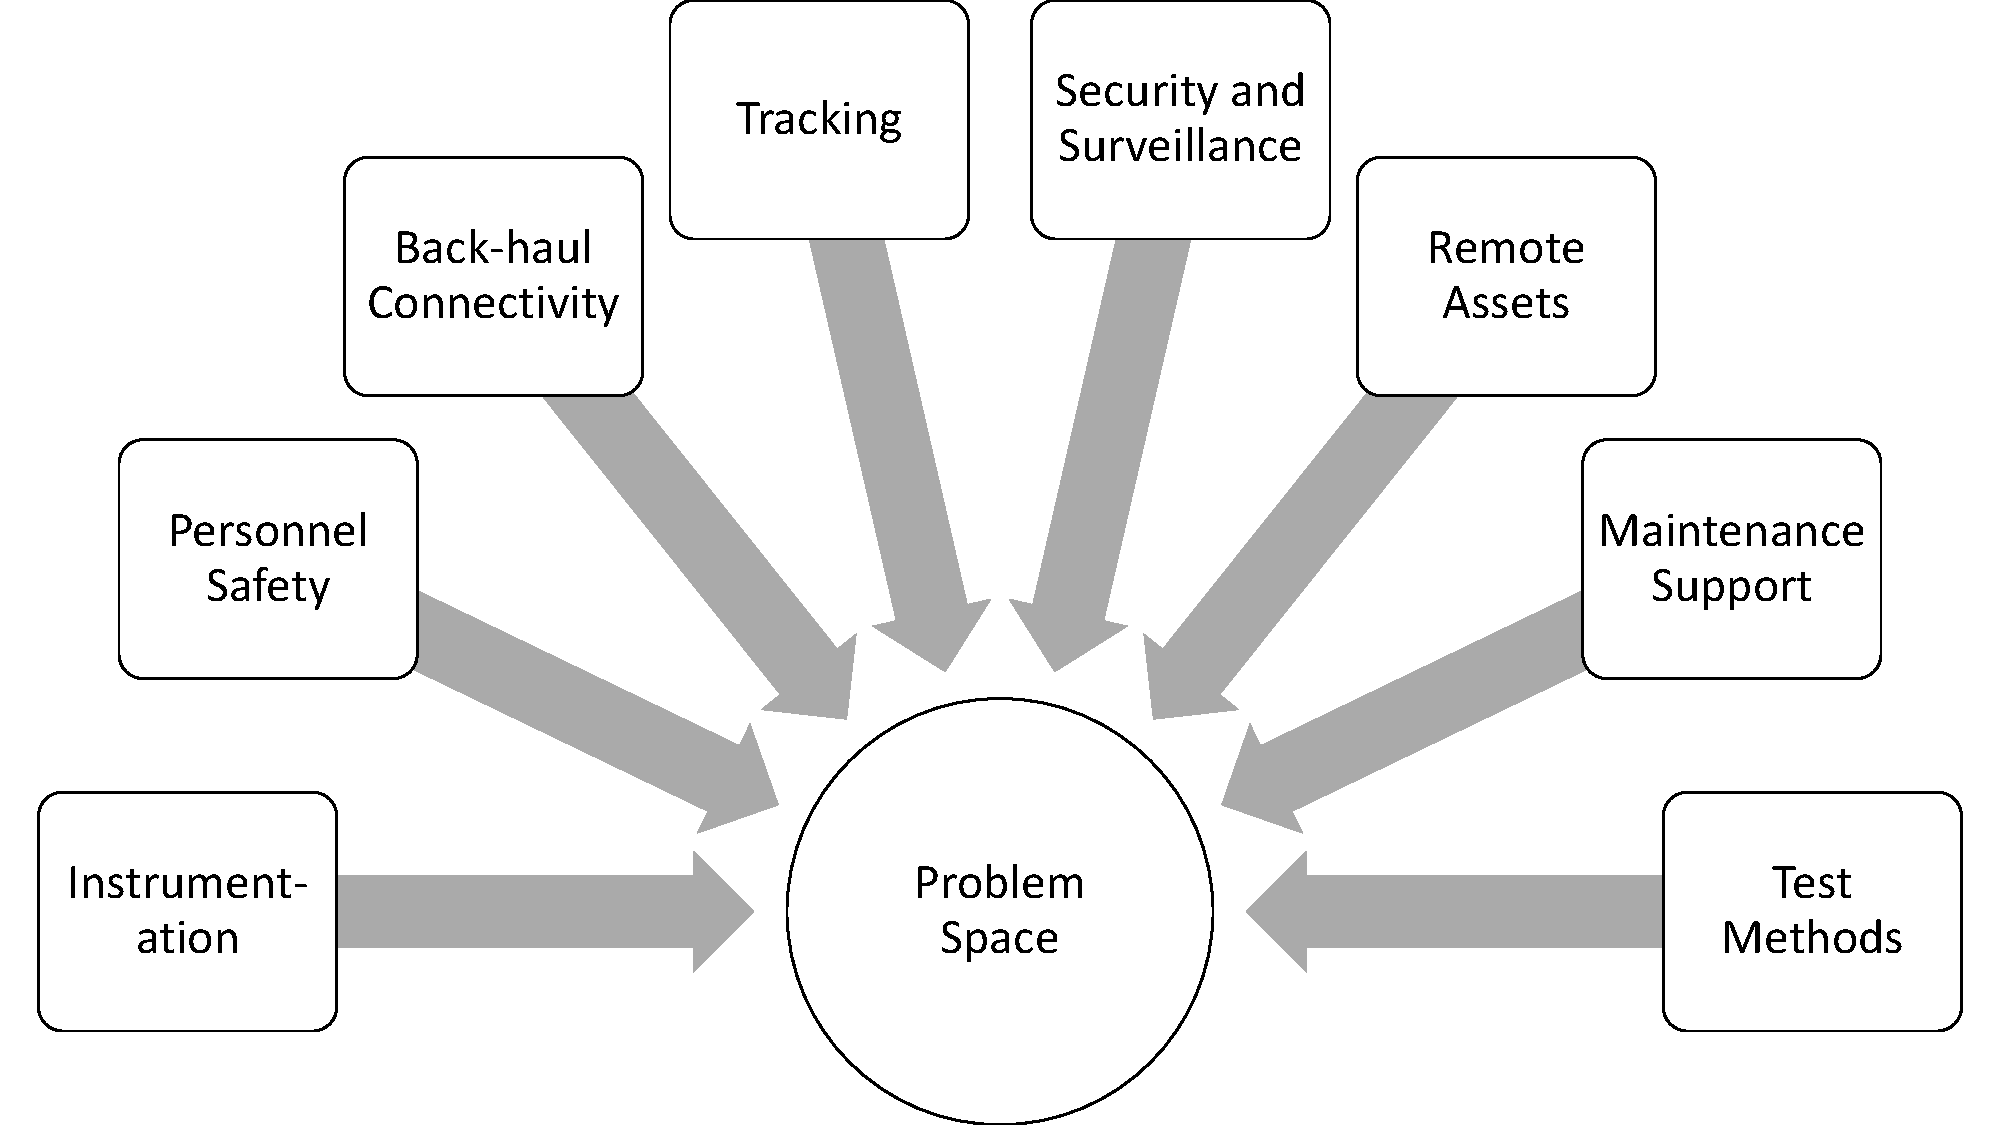
\includegraphics[width=\columnwidth]{./chapter-reswk/figs/probsp}
\caption{Industrial wireless technologies are applicable across most aspects of an industrial operation.}
\label{fig:problemspace}
\end{figure}   

    \subsubsection{Manufacturing Instrumentation}  
    Manufacturing instrumentation includes devices commonly known as sensors and actuators.  Sensors transmit measured variables from the physical process.  Actuators receive manipulation variables from a controller and apply changes to the physical process. This class of application demands typically a very low latency and high reliability communication channel.  
    
    \subsubsection{Personnel Safety}  
    Industrial settings can be hazardous to both humans and machines.  For humans, conditions may arise that pose a substantial risk for injury or death.  For machines, conditions may develop that cause substantial damage requiring extensive repair or replacement.  Prevention of industrial accidents is therefore of paramount importance within factories~\cite{Smith201788}.  Slips, trips, and falls on the same level are commonly cited as lead causes of injury~\cite{Chang2016}. Falls from higher levels are of great concern to the aerospace industry~\cite{Candell2017IWW} as inspection teams must work on elevated levels where falls prove fatal.  Within the oil and gas industry, safety concerns include air toxicity and combustibility in both open and confined spaces where reliable monitoring and reporting save lives. Wireless gas leak detection and leak localization provide important and effective safety enhancements to such systems~\cite{Chraim2016}.  Within smart manufacturing systems where humans and robots work closely and even within traditional robot environments, safety systems provide an added layer of protection to prevent human injury~\cite{Huber:2017:DHI:3029798.3038346}, \cite{Zanchettin2016}.  Within these human-robot environments, it is clear that reliable, low-latency communication is an important aspect of safety implementation, and, as mobility of robots within the factory increases, reliable low-latency wireless networks will become increasingly important to safety implementation.
    
    \subsubsection{Back-haul Connectivity}  The back-haul is generally defined as the network that connects a lower level network to a higher level network \cite{7456186}. Back-haul connectivity is usually characterized by large amounts of transfered data. In industrial environments, various types of back-haul scenarios are needed to be deployed for the operation of industrial communication networks. One can divide the back-haul problem space into three partitions which are i) nearby or indoor back-hauls, ii) distant back-hauls, and iii) geographically remote back-hauls. This categorization is based on the distance over which data is transfered.
    
First, the indoor back-haul networks are used in factory floors or process plants for data transfer between the control level networks to data centers, and higher level application layer networks. Second, the distant back-hauls are used for information transfer between various buildings in a plant where the two ends  may have a line of sight (LOS) or need a non-LOS (NLOS) technology \cite{PS-backhaul}. Finally, the geographically remote back-hauls are used for information transfer between sites in different cities or even countries such as data transfer to headquarters. Various technologies which are currently used for back-haul networks are discussed in \cite{PS-backhaul}.   
    
    \subsubsection{Tracking}
Tracking in industrial environments is employed to follow the states of inventory, personnel, and tools which help in process control and factory management \cite{PS_tracking2}. The focus of this class of the problem space is the set of transmissions related to the tracking process itself and not the recovered data transmissions back to higher levels. Wireless tracking systems are subdivided into the following divisions based on various requirements: i) materials tracking, ii) personnel tracking, iii) tools tracking, iv) inventory management, v) localization, and vi) identification. 

Materials, personnel, and tools tracking is focused on following the state and the location of the tracked item. The selection of the used technology will depend on the tracked item characteristics including its speed, required accuracy level, and scalability \cite{PS-tracking1}. Inventory management includes the decisions related to the change of inventory status over time. Identification and localization are required for the determination of the position and identity of a person or an item at a specific situation or time. It can be important in safety and security related applications. 

The characteristics and applications of various tracking, localization, and identification technologies are discussed in~\cite{PS_tracking2}. These technologies include the use of specific wireless communications technologies like the global positioning system (GPS), and the radio-frequency identification (RFID) or deploying the general-purpose technologies like Wi-Fi, Bluetooth, and the cellular-based technologies. Moreover, examples of the existing products for assets tracking and their performance are compared in \cite{PS-tracking1}.  


    
    \subsubsection{Security and Surveillance}  
    Industrial installations require protection of the physical grounds, the operation, and the data produced from the installation.  This protection requires surveillance of the property and implementation of network security controls. Guidance on selecting which controls are applicable to a specific risk level may be found in~\cite{Stouffer2015}. Assessment of the security robustness of specific wireless technologies is outside the scope of this paper; however, the implementation of physical security controls such as personnel authorization and grounds protection requires transmission of varying amounts of data.  Transmission of such data includes voice traffic, video, and status information.  In some installations, security and surveillance transmissions will coexist with factory instrumentation.  This is sometimes the case with IEEE 802.11 mesh networks carrying voice, video, and instrumentation traffic.  
    
    \subsubsection{Remote Assets} 
Remote monitoring and control extend the range of the management to remote sites, especially in the process industry. Industrial remote communications provide access to widely distributed assets such as well head and pipeline monitoring \cite{PS-remote2}. The main goals of employing remote monitoring and control are minimizing labor cost, improved operations of remote sites, and prevention of  unplanned failures \cite{PS-remote1}. 

The use of wireless networks in remote monitoring and control reduces the installation and maintenance cost significantly. However, the main challenge for industrial wireless remote monitoring and control is security and hence encryption and authentication protocols are deployed. Examples of remote assets communications are discussed in \cite{PS-remote2}.      
    
    \subsubsection{Maintenance Support}  
    Factories require maintenance teams to keep machinery operating efficiently.  Machines may be instrumented with sensors that measure machine health data such as vibration levels or current calibration values.  Using this information, machines can be scheduled for maintenance prior to failure thereby allowing the factory to operate without unexpected interruption.  Maintenance of the factory may also include automation of the building and infrastructure for climate control.  Heating, ventilation, and air conditioning (HVAC) systems can be automated such that the ambient conditions are controlled.  Augmented reality is an emerging technology that promises to bring knowledge to the factory floor allowing maintenance personnel to gain access to information during uncertain situations~\cite{Paelke2014}.  Augmented reality is a high-bandwidth application that requires high-reliability, high-throughput wireless connectivity within the factory.
    
    \subsubsection{Test Methods}  
Industrial control systems are often intolerant of communication faults and network latency, and often require very high transmission reliability~\cite{Zhang2013}. Depending on the purpose of the wireless network (monitoring, supervisory control, feedback control, or safety monitoring), understanding the system performance of the network may be critical. For feedback control and safety monitoring systems, understanding the performance of the network from the perspective of the industrial controller or safety alarm system is essential. Factory operators, system integrators, and control systems designers are rarely experts in wireless communications systems.  Considerations such as electromagnetic propagation, antenna efficiency, path loss exponents, packet error rates, and medium access are often foreign concepts to factory engineers.  If factory engineers are expert in wireless theory and design practice, the information that they need to make educated decisions are usually unavailable.  When available, link quality metrics such as packet loss ratios are informative but can be difficult to understand with complex mesh architectures and routing algorithms.

Moreover, it is generally difficult to measure these quantities for operational networks. The control system designer will only need to know the statistical distribution of latency and reliability of information through the network to design a controller that is robust. Therefore, practical methods for characterizing the performance of the wireless network that do not require an in-depth understanding of wireless communications or electromagnetic wave propagation are needed.

\begin{emphbox}
	A clear need for accessible test methods exists in the wireless cyberphysical systems space in which the tester need not be an expert in wireless communications or radio wave propagation.
\end{emphbox}

    
    \section{Technical Considerations}

    \subsection{Radio Frequency (RF) Environment}
   Using wireless communications in industrial environments requires the knowledge of the RF environment characteristics and their behavior under the added wireless networks. The first step is obtaining and modeling field data in industrial environments. In \cite{Candell2017}, the RF environments of multiple examples of industrial scenarios were studied where models and characterization parameters have been derived. Moreover, theoretical models are proposed to model the RF channel such as the IEEE802.15.4a model including its channel impulse response \cite{A.F.Molisch2004}. In characterizing the RF environments, various parameters should be included, such as the multi-path, the interference sources, the mobility, and shadowing effects. Moreover, the operating frequency band can play an important role based on the required performance and the nature of RF activity in a certain environment.
   
%   Rick: reference NIST-TN-1951 
%    Are things changing in the environment?
%    Multi-path (IEEE 802.15.4a report)
%    What are the interference sources
%    What are the distances between wireless nodes
%    If mobile links or changing environment: shadowing effects
%    Does a mobility model apply to the scene
%    Is it indoor/outdoor?
%    RFBand selection: 900, 2400, 5000
%    mmwave~\cite{Cheffena7565190}
    
    \subsection{Device Characteristics}  
Another important aspect while deploying wireless networks in industrial environments is the used devices characteristics. Typically, the harsh industrial environments in many applications require higher ratings of the used devices. The considered device characteristics include size, weight, power, cost, safety, and ingress protection (IP) ratings. Based on the application requirements and the physical environments, these device requirements are determined.



%Device consideration include size, weight, power, cost, environmental, and safety. When considering the size of the devices
%    IP64-66 rating (Ingress Protection) Rating
%    intrinsic safety rating for combustible environments
%    shock, vibration, heat, humidity, etc.
    
    \subsection{Network Characteristics}
    
Table~\ref{tbl:techreqs} lists requirements typically expected of a network based on its intended purpose and problem domain.  Industrial networks will have three basic characteristics: reliability, latency, and scale.  These characteristics are described in the following subsections.  The numbers listed in the table are based on existing applications.  It is difficult to provide a standard metric for all use cases as each will impose different requirements on the network.  In some cases, the control algorithm can be designed to adapt to information loss and delay, thereby improving the performance of the physical system.

	\subsubsection{Latency} is a measure of the delay that information takes to arrive at its destination.  Latency, $l$, is defined as the measured delay from the time of an event to the time in which knowledge of that event is made available to an application. Using the Open Systems Interconnection (OSI) model as a guide, latency would be measured at the application layer.  In a packaging system, an example of measured latency would be the time between a proximity event and the time knowledge of that event is received by a programmable logic controller. 
    
    \subsubsection{Reliability} is a measure of the likelihood of data loss within the industrial network.  Reliability, $r$, is defined as the probability that a block of transmitted data is delayed long enough to become obsolete or lost due to noise.  Similar to latency, reliability is measured at the application layer thereby ignoring technology-specific issues such as data segmentation and retries similar to the approach taken in the developing 5G cellular networks for machine-to-machine communications~\cite{Holfeld2016}.
    
    \subsubsection{Scale} is a measure of the number of devices that may be deployed within a network without sacrificing reliability or latency. The network size will often dictate the maximum bandwidth allotted to any one node.  The larger the network, the less bandwidth is alloted for transmissions between nodes.  The complexity of a fully interconnect mesh will theoretically exhibit factorial growth in network interconnections.  In practice, signal-to-noise ratios between nodes, programming within the governing network controller, and provisioned constraints will limit the number of interconnections.  Most wireless sensor network specifications such as WirelessHART, ISA100.11a, and Zigbee provide support for large scale deployments; however, in such deployments, the network infrastructure must support the throughput load of the network and the scan rate requirements of the factory application~\cite{Wang7448365}.  The ISA100.11a standard provides support for distributed access points, prescribed routing, and a partitioned architecture to allow for large-scale deployments.

% Requirements table
\begin{table}[!t]
	\centering
	\caption{Industrial control latency, error rate, and scalability considerations for wireless deployments.}
	\label{tbl:techreqs}
	% Table generated by Excel2LaTeX from sheet 'reqs'
\begin{tabular}{llll}
 &
  Latency, $l$ \si{ms} &
  Pr. Loss, $r$ &
  Scale, $s$
  \\
\midrule
Monitoring &
  $l<1000$ &
  $r<10^{-5}$ &
  $s<10,000$
  \\
\midrule
Supervisory Control &
   &
   &
  
  \\
   Flow-based &
  $l<1000$ &
  $r<10^{-6}$ &
  $s<30$
  \\
   Job-based &
  $l<100$ &
  $r<10^{-7}$ &
  $s<10$
  \\
\midrule
Feedback Control &
   &
   &
  
  \\
   Flow-based &
  $l<1000$ &
  $r<10^{-6}$ &
  $s<100$
  \\
   Job-based &
  $l<10$ &
  $r<10^{-7}$ &
  $s<10$
  \\
\midrule
Safety &
  $l<10$ &
  $r<10^{-7}$ &
  $s<10$
  \\
\bottomrule
\end{tabular}%

\end{table}%

    \subsubsection{Interoperability}
    In a factory application, easy integration of devices is essential to  the flow of data through a network. While many wireless standards exist, making physical layer integration of devices within the wireless domain easier, most industrial networks fail to address the application layer well.  WirelessHART describes an application layer interface, while ISA100.11a provides the constructs for such an interface.  ZigBee and Wi-Fi provide neither the interface nor the constructs for an application layer protocol. On the back-haul side of wireless networks which usually begins at a wireless gateway and ends at an automation server, many protocols such as Open Platform Communications (OPC) and Modbus make integration easier; however, again, they fail to specify the interface but instead provide the constructs.  The authors assert that a standardization of the automation interface (gateway to automation server) is needed to provide such interoperability. 
    
    \subsubsection{Security}
    Prescribing security controls within an automation system requires understanding of the risk of not implementing these controls and the impacts of them on the physical process. Work is being undertaken to measure the impacts of cybersecurity controls on the physical process as explained in~\cite{candell2015industrial} and~\cite{candell2015measuring}. In addition, the work is being undertaken to assess the impacts of stealthy attacks as described in~\cite{urbina2016limiting}. NIST Special Publication 800-82 and IEC-62443 provide best practice guidelines for the implementation of a cybersecurity program in an automation system.
    
    \section{Wireless Technology Applicability}
    Many existing wireless technologies could be applied to the use cases in Section II.  Others may be applicable with limitations, and others are not applicable entirely. Table~\ref{tbl:techmap} captures mapping of technologies to applicable use cases.  This table represents assertions by the authors of applicability of wireless technologies to industrial control systems problem domains based on industry practice and original intent of the technology.  The authors assert that the problem domains and wireless technologies included within this table represent the majority  of problems found within industry and the existing technologies that may be applied.  Technologies were evaluated based on original design intent, latency, reliability, energy, and practicality.  Modifications may be made to the listed technologies resulting in applicability to a specified problem; however, possible modifications were not considered.  Very low bit rate (VLBR) wide area networks (WAN) are assumed to have an infrastructure-based  topology and support a bit rate of under 600bps. 
    
% Table generated by Excel2LaTeX from sheet 'mapping'
\begin{table*}[htbp]
	\setlength{\tabcolsep}{1.4pt}
  	\centering
  	\caption{Asserted applicability of wireless technologies.}
  	\label{tbl:techmap}%
  	\begin{adjustbox}{width=\textwidth}
	% Table generated by Excel2LaTeX from sheet 'mapping'
\begin{tabular}{l|l|ccccc|cccccc|cccc|cccc|ccccc|cccccc|ccc|ccc}
\multicolumn{1}{r}{} &
  \multicolumn{1}{r}{} &
  \begin{sideways}Process Monitoring\end{sideways} &
  \begin{sideways}Supervisory Control\end{sideways} &
  \begin{sideways}Feedback Control\end{sideways} &
  \begin{sideways}Alarm Conditions\end{sideways} &
  \multicolumn{1}{c}{\begin{sideways}In-situ Inspection\end{sideways}} &
  \begin{sideways}Factory Monitoring\end{sideways} &
  \begin{sideways}Assembly: Sensing\end{sideways} &
  \begin{sideways}Assembly: Actuation\end{sideways} &
  \begin{sideways}Robots: Supervision\end{sideways} &
  \begin{sideways}Robots: Feedback Control\end{sideways} &
  \multicolumn{1}{c}{\begin{sideways}Quality Inspection\end{sideways}} &
  \begin{sideways}Fall Prevention\end{sideways} &
  \begin{sideways}Confined Spaces\end{sideways} &
  \begin{sideways}Critical Event Detection\end{sideways} &
  \multicolumn{1}{c}{\begin{sideways}Human-Machine Colocation\end{sideways}} &
  \begin{sideways}Nearby or Indoor\end{sideways} &
  \begin{sideways}Distant: LOS\end{sideways} &
  \begin{sideways}Distant: BLOS\end{sideways} &
  \multicolumn{1}{c}{\begin{sideways}Geographically Remote\end{sideways}} &
  \begin{sideways}Indoor Machine Localization\end{sideways} &
  \begin{sideways}Materials in Storage\end{sideways} &
  \begin{sideways}Materials in Production\end{sideways} &
  \begin{sideways}Tools\end{sideways} &
  \multicolumn{1}{c}{\begin{sideways}Personnel\end{sideways}} &
  \begin{sideways}Voice and Video Communication\end{sideways} &
  \begin{sideways}Video Survellience\end{sideways} &
  \begin{sideways}Drone-based Surveillance\end{sideways} &
  \begin{sideways}Grounds Control\end{sideways} &
  \begin{sideways}Spectrum Monitoring Data\end{sideways} &
  \multicolumn{1}{c}{\begin{sideways}Personnel Authorization\end{sideways}} &
  \begin{sideways}Well-head Monitoring\end{sideways} &
  \begin{sideways}Pipeline Monitoring\end{sideways} &
  \multicolumn{1}{c}{\begin{sideways}Tank Level Monitoring\end{sideways}} &
  \begin{sideways}Machine Health Monitoring\end{sideways} &
  \begin{sideways}Building Automation\end{sideways} &
  \begin{sideways}Augmented Reality\end{sideways}
  \\
\multicolumn{1}{r}{} &
  \multicolumn{1}{r}{} &
  \multicolumn{5}{c|}{Flow-based} &
  \multicolumn{6}{c|}{Job-based} &
  \multicolumn{4}{c|}{Safety} &
  \multicolumn{4}{c|}{Back-haul} &
  \multicolumn{5}{c|}{Tracking} &
  \multicolumn{6}{c|}{Security} &
  \multicolumn{3}{c|}{Remote} &
  \multicolumn{3}{c}{Maint.}
  \\
\midrule
\multirow{2}[2]{*}{Home/Office} &
  IEEE 802.11 &
  \CIRCLE &
  \CIRCLE &
  \LEFTcircle &
  \LEFTcircle &
  - &
  \CIRCLE &
  \LEFTcircle &
  \LEFTcircle &
  \LEFTcircle &
  \LEFTcircle &
  \LEFTcircle &
  \fullmoon &
  \fullmoon &
  \LEFTcircle &
  \fullmoon &
  \CIRCLE &
  \CIRCLE &
  \CIRCLE &
  - &
  \LEFTcircle &
  \lightning &
  \lightning &
  \lightning &
  \multicolumn{1}{c}{\lightning} &
  \CIRCLE &
  \CIRCLE &
  \CIRCLE &
  \CIRCLE &
  \CIRCLE &
  \CIRCLE &
  \LEFTcircle &
  \fullmoon &
  \LEFTcircle &
  \LEFTcircle &
  \CIRCLE &
  \CIRCLE
  \\
 &
  IEEE 802.15.1 &
  \fullmoon &
  \fullmoon &
  \fullmoon &
  \fullmoon &
  \fullmoon &
  \fullmoon &
  \LEFTcircle &
  \LEFTcircle &
  \LEFTcircle &
  \fullmoon &
  \CIRCLE &
  \fullmoon &
  \LEFTcircle &
  \fullmoon &
  \fullmoon &
  \fullmoon &
  \fullmoon &
  \fullmoon &
  \fullmoon &
  \fullmoon &
  \fullmoon &
  \lightning &
  \CIRCLE &
  \LEFTcircle &
  \DOWNarrow &
  \DOWNarrow &
  \DOWNarrow &
  \fullmoon &
  \fullmoon &
  \LEFTcircle &
  \fullmoon &
  \fullmoon &
  \fullmoon &
  \LEFTcircle &
  \fullmoon &
  \DOWNarrow
  \\
\midrule
\multirow{4}[2]{*}{Industrial} &
  IEEE 802.15.4 TDMA &
  \CIRCLE &
  \CIRCLE &
  \LEFTcircle &
  \LEFTcircle &
  - &
  \CIRCLE &
  \clock &
  \clock &
  \clock &
  \clock &
  \LEFTcircle &
  \clock &
  \LEFTcircle &
  \LEFTcircle &
  \fullmoon &
  \DOWNarrow &
  \DOWNarrow &
  \DOWNarrow &
  \DOWNarrow &
  \LEFTcircle &
  \lightning &
  \lightning &
  \lightning &
  \LEFTcircle &
  \DOWNarrow &
  \DOWNarrow &
  \DOWNarrow &
  \LEFTcircle &
  \DOWNarrow &
  \fullmoon &
  \CIRCLE &
  \CIRCLE &
  \CIRCLE &
  \CIRCLE &
  \CIRCLE &
  \DOWNarrow
  \\
 &
  IEEE 802.15.4 CSMA &
  \LEFTcircle &
  \LEFTcircle &
  \fullmoon &
  \fullmoon &
  - &
  \CIRCLE &
  \clock &
  \clock &
  \clock &
  \clock &
  \LEFTcircle &
  \clock &
  \LEFTcircle &
  \LEFTcircle &
  \fullmoon &
  \DOWNarrow &
  \DOWNarrow &
  \DOWNarrow &
  \DOWNarrow &
  \LEFTcircle &
  \lightning &
  \lightning &
  \lightning &
  \LEFTcircle &
  \DOWNarrow &
  \DOWNarrow &
  \DOWNarrow &
  \LEFTcircle &
  \fullmoon &
  \fullmoon &
  \LEFTcircle &
  \LEFTcircle &
  \LEFTcircle &
  \CIRCLE &
  \CIRCLE &
  \DOWNarrow
  \\
 &
  IEEE 802.11 TDMA &
  \hexstar &
  \hexstar &
  \hexstar &
  \hexstar &
  - &
  \hexstar &
  \hexstar &
  \hexstar &
  \hexstar &
  \hexstar &
  \hexstar &
  \hexstar &
  \hexstar &
  \hexstar &
  \hexstar &
  - &
  - &
  - &
  - &
  \hexstar &
  - &
  - &
  - &
  - &
  - &
  - &
  - &
  \hexstar &
  - &
  - &
  \hexstar &
  \hexstar &
  \hexstar &
  \hexstar &
  \hexstar &
  -
  \\
 &
  VLBR WAN &
  \CIRCLE &
  \CIRCLE &
  \fullmoon &
  \LEFTcircle &
  - &
  \CIRCLE &
  \clock &
  \clock &
  \clock &
  \clock &
  \clock &
  \clock &
  \fullmoon &
  \fullmoon &
  \fullmoon &
  \DOWNarrow &
  \DOWNarrow &
  \DOWNarrow &
  \DOWNarrow &
  \LEFTcircle &
  \LEFTcircle &
  \LEFTcircle &
  \LEFTcircle &
  \LEFTcircle &
  \DOWNarrow &
  \DOWNarrow &
  \DOWNarrow &
  \clock &
  \fullmoon &
  \fullmoon &
  \fullmoon &
  \fullmoon &
  \fullmoon &
  \LEFTcircle &
  \LEFTcircle &
  \fullmoon
  \\
\midrule
\multirow{3}[2]{*}{Satellite} &
  Geostationary &
  \LEFTcircle &
  \LEFTcircle &
  \fullmoon &
  \fullmoon &
  \fullmoon &
  \fullmoon &
  \fullmoon &
  \fullmoon &
  \fullmoon &
  \fullmoon &
  \fullmoon &
  \fullmoon &
  \fullmoon &
  \fullmoon &
  \fullmoon &
  \fullmoon &
  \fullmoon &
  \fullmoon &
  \LEFTcircle &
  \fullmoon &
  \fullmoon &
  \fullmoon &
  \fullmoon &
  \fullmoon &
  \LEFTcircle &
  \LEFTcircle &
  \fullmoon &
  \LEFTcircle &
  \LEFTcircle &
  \LEFTcircle &
  \LEFTcircle &
  \LEFTcircle &
  \LEFTcircle &
  \fullmoon &
  \fullmoon &
  \LEFTcircle
  \\
 &
  Low-earth Orbit &
  \LEFTcircle &
  \LEFTcircle &
  \fullmoon &
  \fullmoon &
  \fullmoon &
  \fullmoon &
  \fullmoon &
  \fullmoon &
  \fullmoon &
  \fullmoon &
  \fullmoon &
  \fullmoon &
  \fullmoon &
  \fullmoon &
  \fullmoon &
  \fullmoon &
  \fullmoon &
  \LEFTcircle &
  \LEFTcircle &
  \fullmoon &
  \fullmoon &
  \fullmoon &
  \fullmoon &
  \fullmoon &
  \LEFTcircle &
  \LEFTcircle &
  \LEFTcircle &
  \LEFTcircle &
  \LEFTcircle &
  \LEFTcircle &
  \LEFTcircle &
  \LEFTcircle &
  \LEFTcircle &
  \LEFTcircle &
  \fullmoon &
  \LEFTcircle
  \\
 &
  VLBR WAN &
  \LEFTcircle &
  \LEFTcircle &
  \fullmoon &
  \LEFTcircle &
  \fullmoon &
  \clock &
  \clock &
  \clock &
  \clock &
  \clock &
  \clock &
  \clock &
  \fullmoon &
  \fullmoon &
  \fullmoon &
  \DOWNarrow &
  \DOWNarrow &
  \DOWNarrow &
  \DOWNarrow &
  \fullmoon &
  \fullmoon &
  \fullmoon &
  \fullmoon &
  \LEFTcircle &
  \DOWNarrow &
  \DOWNarrow &
  \DOWNarrow &
  \LEFTcircle &
  \fullmoon &
  \fullmoon &
  \fullmoon &
  \fullmoon &
  \fullmoon &
  \LEFTcircle &
  \fullmoon &
  \DOWNarrow
  \\
\midrule
Tracking &
  RFID &
  - &
  - &
  - &
  - &
  - &
  - &
  - &
  - &
  - &
  - &
  - &
  - &
  - &
  - &
  - &
  - &
  - &
  - &
  - &
  \fullmoon &
  \CIRCLE &
  \CIRCLE &
  \CIRCLE &
  \CIRCLE &
  - &
  - &
  - &
  - &
  - &
  - &
  - &
  - &
  - &
  - &
  - &
  -
  \\
\midrule
\multirow{2}[1]{*}{Optical} &
  Indoor Dispersive &
  \hexstar &
  \hexstar &
  \hexstar &
  \hexstar &
  \fullmoon &
  \hexstar &
  \hexstar &
  \hexstar &
  \hexstar &
  \hexstar &
  \hexstar &
  \hexstar &
  \hexstar &
  \hexstar &
  \hexstar &
  \hexstar &
  \fullmoon &
  \fullmoon &
  \fullmoon &
  \hexstar &
  \lightning &
  \lightning &
  \lightning &
  \lightning &
  \hexstar &
  \hexstar &
  \fullmoon &
  \fullmoon &
  \hexstar &
  \fullmoon &
  \fullmoon &
  \fullmoon &
  \fullmoon &
  \hexstar &
  \fullmoon &
  \fullmoon
  \\
 &
  Free-space &
  \LEFTcircle &
  \LEFTcircle &
  \LEFTcircle &
  \LEFTcircle &
  \fullmoon &
  \fullmoon &
  \fullmoon &
  \fullmoon &
  \fullmoon &
  \fullmoon &
  \fullmoon &
  \fullmoon &
  \fullmoon &
  \fullmoon &
  \fullmoon &
  \CIRCLE &
  \CIRCLE &
  \CIRCLE &
  \fullmoon &
  \LEFTcircle &
  \fullmoon &
  \fullmoon &
  \fullmoon &
  \fullmoon &
  \CIRCLE &
  \CIRCLE &
  \fullmoon &
  \fullmoon &
  \fullmoon &
  \fullmoon &
  \CIRCLE &
  \fullmoon &
  \CIRCLE &
  \fullmoon &
  \fullmoon &
  \CIRCLE
  \\
\midrule
\multirow{3}[2]{*}{Cellular} &
  Legacy &
  \LEFTcircle &
  \LEFTcircle &
  \fullmoon &
  \fullmoon &
  - &
  \fullmoon &
  \fullmoon &
  \fullmoon &
  \fullmoon &
  \fullmoon &
  \fullmoon &
  \clock &
  \clock &
  \clock &
  \clock &
  \LEFTcircle &
  \LEFTcircle &
  \LEFTcircle &
  \LEFTcircle &
  \fullmoon &
  \fullmoon &
  \fullmoon &
  \fullmoon &
  \fullmoon &
  \fullmoon &
  \fullmoon &
  \fullmoon &
  \fullmoon &
  \hexstar &
  \LEFTcircle &
  \LEFTcircle &
  \LEFTcircle &
  \LEFTcircle &
  \LEFTcircle &
  \DOWNarrow &
  \DOWNarrow
  \\
 &
  4G &
  \LEFTcircle &
  \LEFTcircle &
  \fullmoon &
  \clock &
  - &
  \fullmoon &
  \fullmoon &
  \fullmoon &
  \fullmoon &
  \fullmoon &
  \fullmoon &
  \clock &
  \clock &
  \clock &
  \clock &
  \LEFTcircle &
  \LEFTcircle &
  \LEFTcircle &
  \LEFTcircle &
  \fullmoon &
  \fullmoon &
  \fullmoon &
  \fullmoon &
  \fullmoon &
  \CIRCLE &
  \CIRCLE &
  \LEFTcircle &
  \CIRCLE &
  \CIRCLE &
  \CIRCLE &
  \LEFTcircle &
  \LEFTcircle &
  \LEFTcircle &
  \fullmoon &
  \fullmoon &
  \fullmoon
  \\
 &
  5G &
  \hexstar &
  \hexstar &
  \hexstar &
  \hexstar &
  - &
  \hexstar &
  \hexstar &
  \hexstar &
  \hexstar &
  \hexstar &
  \hexstar &
  \hexstar &
  \hexstar &
  \hexstar &
  \hexstar &
  \CIRCLE &
  \CIRCLE &
  \CIRCLE &
  \fullmoon &
  \hexstar &
  \hexstar &
  \hexstar &
  \hexstar &
  \hexstar &
  \hexstar &
  \hexstar &
  \hexstar &
  \hexstar &
  \hexstar &
  \hexstar &
  \hexstar &
  \hexstar &
  \hexstar &
  \hexstar &
  \hexstar &
  \hexstar
  \\
\midrule
\multicolumn{1}{l|}{Land-mobile} &
  All types &
  \fullmoon &
  \fullmoon &
  \fullmoon &
  \fullmoon &
  \fullmoon &
  \fullmoon &
  \fullmoon &
  \fullmoon &
  \fullmoon &
  \fullmoon &
  \fullmoon &
  \fullmoon &
  \fullmoon &
  \fullmoon &
  \fullmoon &
  \DOWNarrow &
  \DOWNarrow &
  \fullmoon &
  \fullmoon &
  \fullmoon &
  \fullmoon &
  \fullmoon &
  \fullmoon &
  \fullmoon &
  \LEFTcircle &
  \fullmoon &
  \fullmoon &
  \CIRCLE &
  \fullmoon &
  \LEFTcircle &
  \fullmoon &
  \fullmoon &
  \fullmoon &
  \fullmoon &
  \fullmoon &
  \multicolumn{1}{c}{\fullmoon}
  \\
\midrule
Specialty &
  Leaky Coax &
  \LEFTcircle &
  \LEFTcircle &
  - &
  \LEFTcircle &
  \LEFTcircle &
  \LEFTcircle &
  - &
  - &
  \fullmoon &
  \fullmoon &
  - &
  \fullmoon &
  \LEFTcircle &
  \LEFTcircle &
  - &
  \LEFTcircle &
  \fullmoon &
  \fullmoon &
  \fullmoon &
  \LEFTcircle &
  \CIRCLE &
  \CIRCLE &
  \fullmoon &
  \fullmoon &
  \fullmoon &
  \fullmoon &
  \fullmoon &
  \CIRCLE &
  \fullmoon &
  \CIRCLE &
  \fullmoon &
  \fullmoon &
  \fullmoon &
  \LEFTcircle &
  \LEFTcircle &
  \fullmoon
  \\
\bottomrule
\end{tabular}%

	\end{adjustbox}
	\vspace{3pt}
	\raggedright
	
	Legend: 
	\CIRCLE:~{Technology fully supports problem domain,}
	\LEFTcircle:~{Supports problem domain with practicality, throughput, latency, reliability, or energy limitations,}
	\lightning:~{Energy requirements of assumed battery-powered devices prevent applicability,}
	\clock:~{Latency prevent applicability,}
	\DOWNarrow:~{Throughput prevents applicability,}
	\hexstar:~{Emerging technology or evolution may support problem domain,}
	\fullmoon:~{Not recommended,}
	-:~{Not considered by authors.}
% \newline
% \noindent\makebox[\linewidth]{\rule{\linewidth}{0.4pt}}
% This table represents assertions by the authors of applicability of wireless technologies to industrial control systems problem domains based on industry practice and intent of the technology.  The authors assert that the problem domains and wireless technologies included within this table represent the majority  of problems found within industry and the existing technologies that may be applied.  In some cases, modifications may be made to the listed technologies resulting in applicability to a specified problem.  Very low bit rate (VLBR) wide area networks (WAN) are assumed to have an infrastructure topology. 
% \noindent\makebox[\linewidth]{\rule{\linewidth}{0.4pt}}
\end{table*}%


	\section{Subsequent Work of Note}
	
	Since the investigation conducted regarding industrial wireless requirements as presented here in this thesis, the author and other expanded on the research and published their findings in~\cite{Montgomery2019}.  The requirements presented therein are reproduced in~\ref{reswk:tab:tab6karl}, and justifications for the requirements presented are explained within the reference.  However, while the technical requirements have been updated in the new work, the classes of use cases and mappings of use cases to technologies remained relatively unchanged. In fact, the work in~\cite{CandellRW2017} served as a research source for the subsequent finding in~\cite{Montgomery2019}.  Therefore, the architectural modeling work presented in the following chapter was unaffected.
	
	
	%%%%%%%%%%%%%%%%%%%% Table No: 6 starts here %%%%%%%%%%%%%%%%%%%%
	
	\begin{table}[tbph!]
		\centering
		\caption{Enhanced Wireless User Requirements for the Factory Workcell.}\label{reswk:tab:tab6karl}
		\begin{threeparttable}[t]
		% Table generated by Excel2LaTeX from sheet 'FromKarl2019'
\begin{tabular}{|p{5.715em}|p{4.855em}|c|c|c|c|c|}
	\toprule
	\multicolumn{2}{|p{10.57em}|}{\textbf{User Requirement}\tnote{1,2}} & \multicolumn{1}{p{4.355em}|}{\textbf{Class 0:}} & \multicolumn{1}{p{4.355em}|}{\textbf{Class 1:}} & \multicolumn{1}{p{4.355em}|}{\textbf{Class 2:}} & \multicolumn{1}{p{4.355em}|}{\textbf{Class 3:}} & \multicolumn{1}{p{4.355em}|}{\textbf{Class 4:}} \\
	\midrule
	\multirow{2}[4]{*}{Latency (ms)} & Typical & 4     & 4     & 20    & 4     & 50 \\
	\cmidrule{2-7}\multicolumn{1}{|r|}{} & Minimum & 0.5   & 0.25  & 4     & 0.5   & 4 \\
	\midrule
	Reliability\tnote{3} & Typical & -7    & -7    & -7    & -7    & -6 \\
	\cmidrule{2-7}(Pr. Loss) & Minimum & -7    & -7    & -7    & -7    & -7 \\
	\midrule
	Scale & Typical & 8     & 10    & 10    & 1     & 100 \\
	\cmidrule{2-7}(\# of links) & Maximum & 16    & 30    & 30    & 4     & 300 \\
	\midrule
	\multirow{2}[4]{*}{Range (m)} & Typical & 10    & 10    & 10    & 10    & 10 \\
	\cmidrule{2-7}\multicolumn{1}{|r|}{} & Maximum & 30    & 30    & 30    & 30    & 30 \\
	\midrule
	\multirow{2}[4]{*}{Payload (B)} & Minimum & 6     & 8     & 8     & 8     & 12 \\
	\cmidrule{2-7}\multicolumn{1}{|r|}{} & Maximum  & 24    & 1024  & 1024  & 1024  & 33000 \\
	\midrule
	Update Rate & Typical & 125   & 125   & 25    & 125   & 10 \\
	\cmidrule{2-7}(Hz)  & Maximum & 1000  & 2000  & 125   & 1000  & 125 \\
	\bottomrule
\end{tabular}%

		\vspace{3pt}
		\raggedright		
		\begin{tablenotes}
		\item[1] This table has been adapted from~\cite{Montgomery2019}. 
		\item[2] The use case classes are defined as follows: Class 0: Safety, Class 1: Closed Loop Regulatory Control, Class 2: Closed Loop Supervisory Control, Class 3: Open Loop Regulatory Control ,and Class 4: Alerting Monitoring.		
		\item[3] The reliability specifications presented indicate a probability of information loss (not packet loss) where the probability is $10^X$ where $X$ is the number indicated.
		\end{tablenotes}
		\end{threeparttable}
	\end{table}
	
	%%%%%%%%%%%%%%%%%%%% Table No: 6 ends here %%%%%%%%%%%%%%%%%%%%	

    
	\section{Conclusions}\label{sec:conclusion}
    
    This work represents a step toward employing wireless technologies in industrial environments where all classes of problems which wireless technologies can be used to solve have been comprehensively and collectively discussed. The success criteria and the technical aspects for employing wireless technologies in various scenarios have been considered briefly. More work is needed where success criteria are to be quantified and prioritized for various industrial scenarios. More detailed discussion is needed regarding technical considerations while employing wireless networking, including the physical environmental aspects such as the factory floor parameters, obstructions, data models, and interaction between various items within the factory floor. Finally, a mapping between technologies and the discussed problem classes has been introduced to highlight various industrial problems which can be solved or need more work while employing wireless technologies. Multiple comparisons between the current technologies exist in the literature. However, this work initiates consideration of the problem space where wireless technologies are employed. NIST has introduced this work while continuing to develop its capabilities as described in~\cite{candell2015measuring} to explore applicability of wireless technologies to specific industrial scenarios capable of replication within a laboratory space. An RF channel emulator is used to simulate the RF environment to include fading and multipath. A technical working group was created to directly address the needs of the wireless users employing wireless within their factories.





\chapter{Workcell Architectural Decomposition}\label{chapter:sysml}

\chapterintro*

Smart Manufacturing provides a vision of future manufacturing systems that incorporate highly dynamic physical systems, robust and responsive communications systems, and computing paradigms to maximize efficiency, enable mobility, and realize the promises of the digital factory.  Wireless technology is a key enabler of that vision. A comprehensive graphical model is developed for a generic wireless factory work-cell which employs the Systems Modeling Language (SysML), a standardized and semantically rich modeling language, to link the physical and network domains in such a cyber-physical system (CPS). Our model identifies the structural primitives, interfaces, and behaviors of the highly-connected factory work-cell in which wireless technology is used for significant data flows involved in control algorithms. The model presented here includes parametric definitions to encapsulate information loss, delay, and mutation associated with the wireless network, and it identifies pertinent wireless information flows.  Use of this model is helpful in communicating architecture, interfaces, limitations, and sources of information within a workcell.  The model was developed to provide a perspective of the smart manufacturing workcell which did not yet exist.

\section{Introduction} \label{sysml:sec:intro}    
The fourth industrial revolution promises unparalleled productivity and capability advances in manufacturing. To support the manufacturing industry in this conversion, various programs have been established in several countries such as Smart Manufacturing in the U.S.~\cite{SmartManuf} and Industry 4.0 in Europe~\cite{Industry40, cpsInd4.0}. Propelled by economic pressure toward greater efficiency, factory agility, and product customization, future factories will have the technological ability to adapt to customer demands quickly, modify manufacturing processes automatically based on quality feedback, and fabricate products with a reduced environmental impact.  Technological advances required for smart manufacturing to be successful include collaborative and mobile robotics~\cite{indRobot2017}, distributed machine autonomy based on artificial intelligence \cite{ManufAI2009}, improved process observability~\cite{IIoToverview2018}, and a high degree of interconnectivity among automation resources~\cite{ieMag2018}. Work-cells are self-contained units of operation within a factory~\cite{CHEN2001199, JMarvel2017, 6059204}.  These work-cells are composed of various machines, conveyors, motors, edge devices, and robots.  Robots will work together and with people to accomplish complex tasks or to tending to other machines within the work-cell.  Robots will have the ability to roam between work-cells within a factory, learn their roles quickly, become aware of edge devices, and communicate with other actors within the work-cell to accomplish their goals. Efficient communications between robots and the other players in the work-cell are essential to the fulfillment of the robot-related tasks.



Current manufacturing architectures use wired connections through field-bus and industrial Ethernet protocols for sensing and real-time control~\cite{etherCAT, indPrinter}.  Indeed, through advances in time-sensitive networking, many of the promises of smart manufacturing are being realized; however, the true goals of smart manufacturing require a large deployment of sensing and actuation devices and mobile, perhaps autonomous, robotics actors~\cite{ieMag2018}.  The use of wires precludes mobility and makes deployment of edge devices more expensive as each  requires power, cables, and conduit for communication. By adopting wireless for both sensing and control of machines within the work-cell, a lower-cost, untethered operation is achievable\footnote{The power for untethered operation can be achieved through the use of rechargeable batteries to power the untethered machine or robot for enough operating period.}. Once wireless is adopted as the primary mode of communication, questions arise as to the required latency, reliability, and scale of the wireless network especially when the network is used for the control of machines and the assurance of safety~\cite{ieMag2018}. 

The work presented here addresses the present need for a comprehensive architectural model of the factory work-cell in which wireless is a preferred mechanism for carrying information within the work-cell. We begin with an architectural analysis of the future collaborative work-cell that includes edge devices, robots, vision systems, and supervisory controllers. Our architectural analysis includes structural components, information flows, and parametric elements of the work-cell. We identify factors that limit reliability, latency, and scalability of the wireless network, and we conclude with a discussion of significant information flows. Significant information flows are defined as operationally critical or safety-related.  Our contributions are:

\begin{itemize}
	\item[$\rhd$] First, we develop a comprehensive and extensible architectural model using the Systems Modeling Language (SysML) that provides primitives for describing the physical and networking components of a work-cell with parametric constraints\footnote{We make the model publicly available for download. A valid license of MagicDraw 18.5 is required to use the model.  A web-based report of the model is provided for read-only access.};
	\item[$\rhd$] Second, we provide a framework for analyzing cross-domain interactions of complex wireless work-cell deployments; and
	\item[$\rhd$] Third, significant information flows are identified, annotated with rate constraints.
\end{itemize}

The remainder of this paper is organized as follows:  In Section~\ref{sysml:sec:related-work}, previous related work is discussed and our motivation for constructing a model is presented.  A brief introduction to systems modeling is presented in Section~\ref{sysml:sec:systemsmodeling} and provides a primer on the SysML language. The conceptual architecture of the model providing a concept-of-usage is proposed in Section~\ref{sysml:sec:conceptual}, followed by a detailed exposition of each package in Section~\ref{sysml:sec:detailed-model}.  Then, in Section~\ref{sysml:sec:wireless-infoflows}, significant information flows are discussed through introducing a case study. Section~\ref{sysml:sec:conclusion} concludes the paper and identifies opportunities for future research.

%\section{Related Work}\label{sysml:sec:related-work}
%
%Current modeling work on factory work-cells is mainly aimed at defining and characterizing the subsystems, such as human staff, robots, and machine tools, in individual applications. By following blueprints (schematics) of production tasks, the work flow can be divided into separate assignments which are distributed by a task dispatch system to individual machines~\cite{IkeaBot}. Analytical models are thus obtained for performance analysis in work-cells. As an example, a mathematical model for real-time performance analysis of a gantry work-cell with robots is established with the timing and the randomness of tasks and disruptions are captured  \cite{8098604}. In \cite{OU2017212}, the same model is used to investigate the system natural properties such the system cycle and waiting times and to identify bottlenecks through studying the sensitivity of each machine. Similarly, the steady state analysis for production lines with uncertainties is performed through various decomposition methods~\cite{Colledani2013,doi:10.1080/00207543.2012.713137,doi:10.1080/00207540500385980}. In \cite{Colledani2013}, a decomposition method is presented for the analysis of continuous flow lines. The presented model is used to analyze flow lines with single and multiple failure mode machines and machines subject to aging and having up and down times. In \cite{doi:10.1080/00207543.2012.713137}, a model to evaluate the performance of transfer lines with unreliable machines and finite transfer-delay buffers is presented. A decomposition method is introduced to model the transfer line, using the general-exponential distributions instead of the exponential distributions to approximate the repair time distributions of the fictitious machines. In \cite{doi:10.1080/00207540500385980}, the authors present a model for evaluating the production rate and distribution of inventory of a closed-loop manufacturing system with unreliable machines and finite buffers. The model accounts for the different sets of machines that could cause blockage or starvation to other machines. In \cite{QChang,Liu2012}, the performance analysis modeling for serial production lines with disruptions is explored by studying the impact of each individual downtime event in terms of permanent production loss and financial cost. These analytical models generally work well for simple systems with small number of components or few interactions between various equipment. Also, the analytical models can be used to abstract industrial systems to understand various performance trends without studying various details. As a result, we introduce a comprehensive model that include network and production impacts on the industrial work-cell.  
%
%Furthermore, the reconfigurable work-cell architecture is widely considered for automated manufacturing. The main advantage of reconfigurable work-cells lies in the flexibility of reconfiguration of work-cell components to adapt to varying production requirements where the assembly of the work cell is optimized for each specific task~\cite{CHEN2001199}. In the work-cell that hosts robots, robots are installed therein to allow for autonomous configuration within their workspace \cite{8023523,10.1007/978-3-319-65151-4_10,6059204}. Approaches and performance criteria for reconfigurable robotic systems have recent developments in control architectures to achieve various levels of reconfigurability \cite{Fulea}. The National Institute of Standards and Technology (NIST) has defined a Network of Things (NoT) model which can depict the structure of work-cells by a group of NoT building blocks and model the behaviors of individual components in a work-cell~\cite{NIST800-183}.  The NIST NoT model is focused primarily on sensor networks and the collection of data.  Actuation is cursorily noted, and, as such, cross-domain interactions between the physical system and the network are not addressed. Several other robotic work-cell architectures are discussed in the literature. In \cite{OpenArch}, a reference model for a control system functional architecture applied to open architecture robot controllers is presented. In \cite{CARPANZANO2007435}, a methodology to develop self-adaptive factory automation solutions is illustrated, using a novel modular simulation based method. With the increase in complexity and reconfigurability of work-cells, studying various production criteria and networks impacts requires introducing new models to capture these interactions and to be abstract enough to model different configurations and scenarios of industrial work-cells.  
%
%In a work-cell model, data flows are used to capture the trajectory of system information exchange between work-cell components and identify their roles in specific operations~\cite{OpenArch}. For example, safety-related operations employ the vision system and various proximity sensors that generate proximity data and transmit them to the safety manager to define safety zones in an automotive assembly work-cell~\cite{safeeye}. 
%In another example, data flows are enabled in a work-cell to capture human operator gestures from embedded cameras in human-robot collaborations~\cite{cobotcell}. These gestures can be later regenerated in simulators based on the transmitted position data from the field to optimize work-cell safety operations~\cite{gesture}. Currently, most of the work-cell information in these scenarios are transmitted by wired networks. Wireless networks have gained increasing interests to enable data flows in the highly connected work-cells. Wireless standard bodies have proposed their network reference models in factory environments which include the work-cell cases in the data-centric architecture~\cite{ETSI889, KPItable}. In these models, individual work-cells are treated as a subnetwork of field instruments attached with data aggregations that manage network connections and transfer data traffic to edge and cloud servers in various applications. Wireless connections are featured with flexible network topology to agree with a variety of transmission needs, especially in reconfigurable work-cells. Meanwhile, data traffic flows are characterized by select performance metrics, such as transmission latency and link reliability, to categorize industrial use cases~\cite{KPItable}. 
%
%Current modeling efforts set the boundaries of their systems of study at the edge devices without further discussions on the impact of wireless performance on the operations of industrial systems. For example, the abstracted disruptions in \cite{QChang,Liu2012} that cause plant downtimes may include wireless network impacts which are not yet treated distinguishably with specific characteristics of wireless networks. As indicated by the earlier empirical studies~\cite{LIU2017412}, such physical systems may have different responses to network performance which will vary with the operational configuration such as the served ``application'' and the deployed control algorithms. In this paper, we incorporate the features of wireless communications networks into the modeling architecture of physical work-cells such that cross-domain interactions may be studied.  Prior to introducing the model for wireless incorporation, we first provide the reader an introduction to SysML in the following section.
%
%\section{Systems Modeling Using SysML}\label{sysml:sec:systemsmodeling}
%
%The goal of modeling a system is the capture of knowledge of a process in a simplified way~\cite{SysModel2004}. A secondary goal of a system model is to provide a level of abstraction that may allow for the discovery of new knowledge such as how two systems will interact. There are multiple ways of designing and presenting system models. Well-behaved systems can be represented by a system of equations using mathematical tools~\cite{SimModel1999}. Such models provide excellent constraint definition, but lack the semantics to describe architecture and detailed information flow.
%Moreover, by deploying functional block diagrams, we are able to capture major functional components and flow of information or material. As shown in Fig.~\ref{sysml:fig:fbd-system}, a physical process interacts with a control system through a wireless network.  Measured values, $Y$, from sensors flow to the controller through a wireless network and arrive at the controller delayed and modified, $\bar{Y}$. Similarly, commands, $U$, flows from the controller to the actuators through the wireless network. Such diagrams may be used to model feedback control systems in which the origination and routing of information are immaterial for study. However, the architecture and interfaces remain at a very high level of abstraction making analysis difficult. In such cases, delay and loss using such tools are often modeled stochastically. Using architectural diagrams helps identify components, interfaces, and information flow. For factory systems, architectural block diagrams are often manifested as schematics. However, such diagrams have their own limits in industrial practices. On one hand, they lack the semantics necessary to describe the constraints that formal equations and functional block diagrams offer. Meanwhile, they also lack the capability of capturing behaviors or complex interactions between the physical system and the information infrastructure such as a wireless network. 
%
%\begin{figure}
%	\centering
%	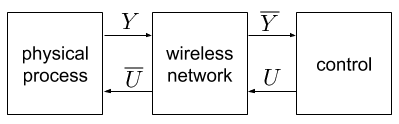
\includegraphics[width=0.65\columnwidth]{./chapter-sysml/diagrams/fbd-system}
%	\caption{Functional block diagram of a cyber-physical system in which a physical process and an automation system interact through a wireless network.}
%	\label{sysml:fig:fbd-system}
%\end{figure}
%
%An alternative to schematic diagrams is SysML~\cite{SysML2017}. SysML is a general purpose modeling language that is often used for model-based systems engineering (MBSE) practice within industrial systems~\cite{MBSEandSysML}. SysML provides structural, behavioral, and parametric semantics for the analysis of complex systems. For examples, systems analysis using SysML enables capturing and communicating system requirements and design which include hardware, software, firmware, information flows, and processes with graphical notations. Within the factory automation industry, engineers are adopting SysML in the form of MBSE to develop realizable operational models of the factory and data flow processes. MBSE models address verification of design through executable simulations depending on the modeling tool.  The SysML specification is defined in~\cite{SysML2017}.  In SysML, the basic semantic constructs of the language are Packages, Blocks, Ports, Interfaces, and Constraints, in addition to the constructs provided by the Unified Modeling Language (UML). Packages are logical grouping of model elements. Package relationships are captured using the package diagram (PKG). Relationships of these constructs are captured in the block definition diagram (BDD).  The internal composition and connectivity of parts are captured in the internal block diagram (IBD). SysML includes other types of diagrams and semantic constructs that are not required for this analysis and are not explained here. The SysML model is comprehensive; however, the size and number of diagrams within the model are too extensive to include within this paper.  Therefore, the reader is encouraged to explore the SysML model defined in~\cite{SysML.Candell2018}.  A useful primer on SysML may be found in~\cite{Friedenthal2015.SysML}. 
%
%Examples of the use cases and methodologies of using different graphical models for the analysis of manufacturing systems are explored in~\cite{Lutjen2015.GramosaMethod,Luder2011.GraphicalModeling,Jia2013.GraphicalModeling,Alvarez2013.GraphicalModeling}.  In~\cite{Quinsat2017.SysML}, SysML is used to capture both composition and behavior of an additive manufacturing work-cell.  A survey of applying graphical modeling languages in capturing information flows within a product service system which may be applied to manufacturing enterprises~\cite{Durugbo2011.GraphicalModeling}.  Our approach compliments these previous examples by combining the operational and wireless information transport systems together in a single model, thereby facilitating a single model that may be used for simulation and other systems engineering analyses.
%
%While various architectures for the work-cell exist as exemplified in the literature, a common language and framework for communicating architecture and information flow has not been established for cross-domain interactions between the manufacturing system and its supporting communication networks.
%SysML contains the semantics for such engineering capture and provides an industry accepted language for communicating composition, interfaces, and information flow. Moreover, SysML provides the semantics for assigning properties to any model element such that those properties are made  available for analysis using other tools such as Prot\'eg\'e \cite{StanfordUniversity.Protege} and the Web Ontology Language (OWL) \cite{W3C2012.OWL}.
%It is important to understand that while SysML provides semantics for a formal capture of architecture, information flow, and parametric constraints, it may also be used for a higher-degree of abstraction provided by the functional block diagrams.  

\section{Conceptual Representation} \label{sysml:sec:conceptual}
The remainder of this work describes a reusable model for representing a comprehensive wireless factory work-cell using the semantic constructs of SysML.  We now follow with an exposition of our model beginning with the conceptual model followed by a detailed description of each component within the model. When discussing the model, the SysML term, \textit{block}, is omitted for the sake of brevity where the meaning is clear. 
\subsection{Packages}
The factory work-cell is decomposed into one general and nine major structural packages as shown in Fig.~\ref{sysml:fig:pdd-workcell}.  Packages include major logical groupings of structure within the model.  These packages are enumerated in the following paragraphs.

\begin{figure}[t]
	\begin{center}
		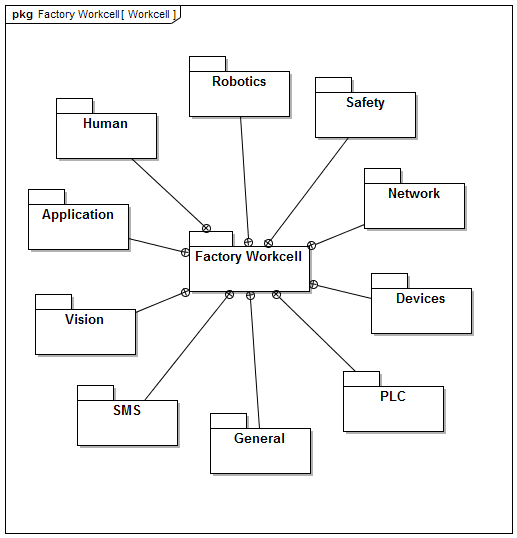
\includegraphics[width=0.95\columnwidth]{./chapter-sysml/diagrams/pkg__Factory_Workcell__Workcell}%
		\caption{SysML package diagram showing the logical containment of the factory work-cell structural elements.}%
		\label{sysml:fig:pdd-workcell}
	\end{center}
\end{figure}


\subsubsection{General} A set of reusable structural elements that is used for conceptual modeling or extended to produce more complex model elements.  Each of the sub-packages within the General package extends basic features.  The sub-packages within General include time and constraints for data, electro-magnetics, and motion.

\subsubsection{Network} Describes the components, blocks, interfaces, and limiting factors of the industrial wireless network (IWN).  The IWN is modeled as the radio channel and the services provided by the network. Limiting factors are modeled as parametric equations associated with the radio channel and the services.

\subsubsection{Application}  This package contains the model elements describing a component of behavioral functionality typically implemented within software or firmware but could be implemented in hardware.  It describes the features and constraints of factory operation such as the logic of a supervisory controller or the feedback controller of a robot arm.  The Application sets the performance requirements of the wireless network, i.e., the factory network performance requirements are derived from the requirements of the applications deployed to a work-cell.

\subsubsection{Devices} Describes the types of devices found within the factory work-cell to include any device that interacts with the environment such as wired and wireless input-output (IO) devices including sensors and actuators.

\subsubsection{Robotics} Describes the computational and communicative components of robot control including sensing, actuation, and command.  Description of the robot itself is inconsequential to communication and therefore not included in the model.

\subsubsection{PLC} Describes the supervisory control components commonly handled by one or more programmable logic controller (PLC) components.  This package includes the elements responsible for coordination of actors and handling of most input-output.

\subsubsection{Safety} Describes the allocation of safety qualities typically included in the supervisory controller.  The Safety package includes devices, monitoring, and actuation of the safety behaviors within the factory work-cell.

\subsubsection{Vision} Describes the allocation of features to optical monitoring and tracking which are typical to the collaborative robotic work-cell.

\subsubsection{Spectrum Monitoring System (SMS)} Describes the qualities and interfaces of a factory spectrum monitoring system projected into the factory work-cell.  The SMS includes monitoring nodes and agents localized to the work-cell and connected to the automation system for real-time adaptation to changing multi-path and interference. 

\subsubsection{Human} Describes the features associated with human beings such as human motion, tasks, and carried equipment such as portable computing and communication devices.
\vspace{3mm} 

Several examples of how to use the model are provided within the model\cite{SysML.Candell2018}.  Examples include: a robotic force-torque leader-follower, a robotic force-torque limiter, a collision avoidance, and a robotic pick and place work-cell.  The parametric constraints are provided as examples and are intended to be used for communication to project stakeholders or replaced with executable computer code such as MATLAB or Python scripts, thereby making the model useful for simulation depending on the modeling tool selected.

\begin{figure*}
	
	\centering
	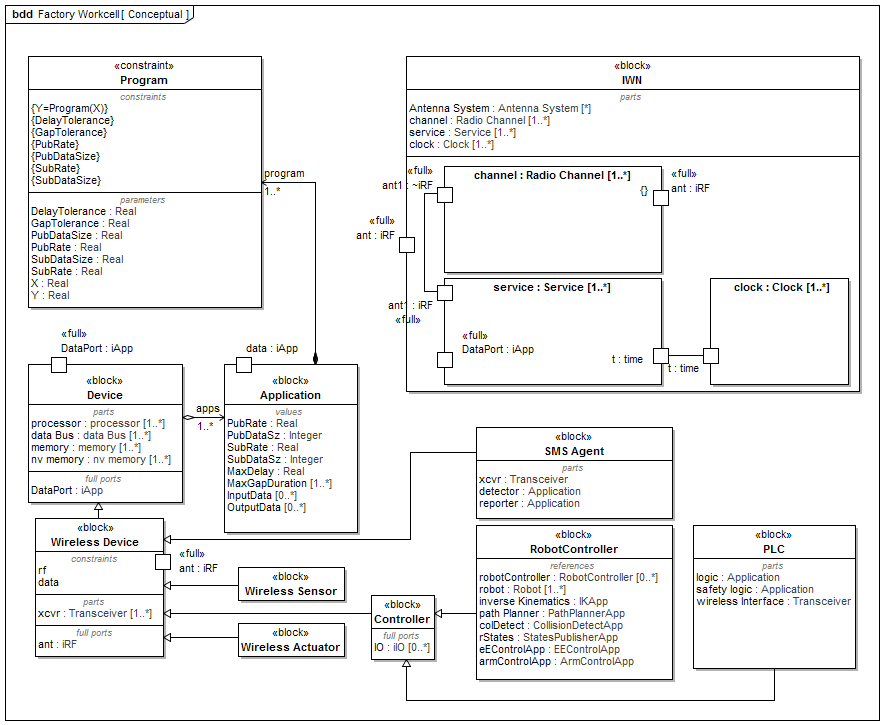
\includegraphics[width=0.97\textwidth]{./chapter-sysml/diagrams/bdd__Factory_Workcell__Conceptual}
	%
	\caption{Architecture of the conceptual work-cell captured as a SysML block definition diagram.  In this diagram, only the most generalized blocks necessary to construct a work-cell scenario are shown.  More application-specific scenarios may be developed by deriving new blocks from the constructs shown here. The shapes and connectors used for expressing this model are defined in the SysML specification\cite{SysML2017}. }
	%
	\label{sysml:fig:conceptual:bdd}
	
\end{figure*}

\subsection{Conceptual Architecture}\label{sysml:sec:architecture}
The conceptual architecture of the wireless work-cell model is depicted in Fig.~\ref{sysml:fig:conceptual:bdd}. All the packages are included in this architecture, and the connections and relations between blocks are defined using the SysML semantics. This figure serves to orient the reader during the presentation of detailed model decomposition in Section~\ref{sysml:sec:detailed-model}. The work-cell model is composed of at least one Industrial Wireless Network (IWN) block and at least one Device block. More IWN blocks are used when multiple wireless networks coexist within the industrial work-cell. Applications are associated with Devices and performance constraints are applied to Applications. In this model, the Wireless Device is a subclass of Device, and the Controller is a further derivation of the wireless device. Moreover, the Controller is an abstract specialization of a wireless device that represents all types of devices intended to control other processes. The behaviour of a PLC or Robot is represented through two packages in the model. The production related behaviour is represented through the corresponding packages and the connectivity behaviour is represented through Devices such as the Robot Controller and the PLC which are special classes of Wireless Device containing all of the structure and behavior of the wireless device. Finally, an often overlooked component of any industrial wireless deployment is the spectrum monitoring system represented by the SMS Agent. Blocks in the model communicate through ports such as the \textit{ant} port which represents the antenna or waveguide interface.  Composition is further implied by the parts, constraints, and parameters associated with each block. These are listed within the compartments of each block.

\section{Detailed Model Decomposition}\label{sysml:sec:detailed-model}
In this section, we describe in detail the decomposition of the model packages. The decomposition of each package includes the properties and the components of the package where the relation between the package and physical industrial work-cells is illustrated. Moreover, some of the packages may have various types with different properties and hence sub-packages are defined for these packages. This section also includes a general explanation of the packages rules in the work-cell and the behavioral interactions between the packages.      

\subsection{General Package}
The General package contains the reusable elements of the model.  In particular, the General package contains elements that are not particular to any one work-cell component but can be reused or applied across several.  The concepts of time, clocks, and synchronization are included within General.  Moreover, several types of constraints are defined.  

\subsubsection{Time}
Time is an important construct within communication systems as well as industrial control systems.  Time is realized as a set of one or more clocks. A work-cell will contain one to several clocks typically embedded within each device to allow those devices to synchronize to a common clock. The local clocks within the work-cell devices will synchronize to a master reference clock and usually one with a high degree of precision, accuracy, and stability.  The degree to which the local clocks synchronize to the master will depend on the requirements of the applications that the local clocks serve.  Clock synchronization can be costly in power, size, and monetary cost of the devices, but it may be necessary depending on the applications using a clock.  Clock performance is a key driver of size and power consumption, and synchronization of clocks across a wireless network can be a challenge and is a highly studied field~\cite{ClockSync.Mahmood2017,ClockSync.Geetha2017}. Moreover, the Time package includes a constraint, Clock Performance, to represent the production of time and synchronization with a master clock. 

\subsubsection{Constraints}\label{sysml:sec:general:constraints}
Constraints provide limitations on the performance of an element within the model.  Within General, several constraints are defined which may be applied to any block within the model. These constraints include motion constraints, radio channel constraints, and networking constraints as shown in Fig.~\ref{sysml:fig:constraints:motion} through \ref{sysml:fig:constraints:network}.  

\paragraph{Motion Constraints}\label{sysml:sec:constraints:motion}

%\begin{figure}[tbp]
%	\centering
%	\subfloat[Motion Constraints\label{sysml:fig:constraints:motion}]{%
%		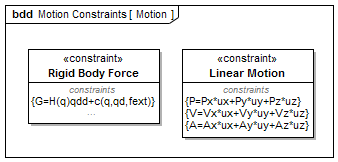
\includegraphics[width=0.95\columnwidth]{./chapter-sysml/diagrams/bdd__Motion_Constraints__Motion}}
%	\hfill
%	\subfloat[Radio Channel Constraints\label{sysml:fig:constraints:radio}]{%
%		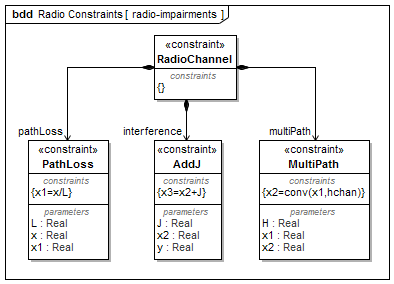
\includegraphics[width=0.95\columnwidth]{./chapter-sysml/diagrams/bdd__Radio_Constraints__radio-impairments}}
%	\hfill
%	\subfloat[Networking Service Constraints\label{sysml:fig:constraints:network}]{%
%		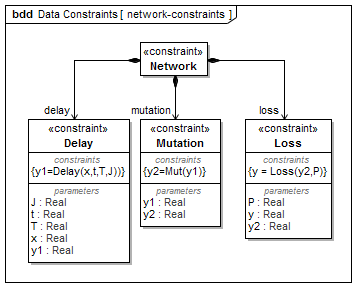
\includegraphics[width=0.95\columnwidth]{./chapter-sysml/diagrams/bdd__Data_Constraints__network-constraints}
%	}  
%	\caption{Generalized network constraints consisting of rigid body motion~\protect\subref{sysml:fig:constraints:motion}, the radio channel~\protect\subref{sysml:fig:constraints:radio} and the network services~\protect\subref{sysml:fig:constraints:network}.}
%	\label{sysml:fig:general:constraints}      
%\end{figure}

\begin{figure}[ht]
	
	\centering
	
	\begin{subfigure}{.8\textwidth}
		\centering
		% include first image
		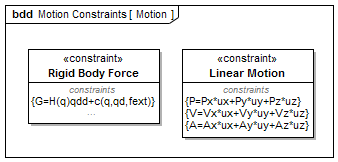
\includegraphics[width=.8\linewidth]{./chapter-sysml/diagrams/bdd__Motion_Constraints__Motion}  
		\caption{Motion Constraints}
		\label{sysml:fig:constraints:motion}
	\end{subfigure}

	\begin{subfigure}{.8\textwidth}
		\centering
		% include second image
		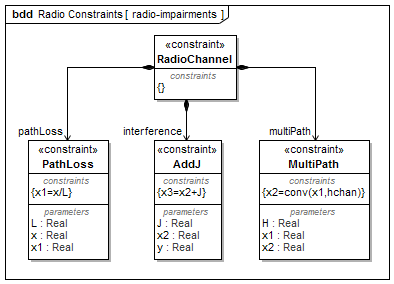
\includegraphics[width=.8\linewidth]{./chapter-sysml/diagrams/bdd__Radio_Constraints__radio-impairments}  
		\caption{Radio Channel Constraints}
		\label{sysml:fig:constraints:radio}
	\end{subfigure}
	
	\begin{subfigure}{.8\textwidth}
	\centering
	% include second image
	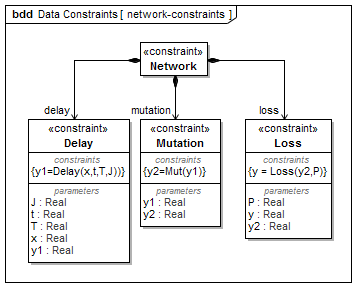
\includegraphics[width=.8\linewidth]{./chapter-sysml/diagrams/bdd__Data_Constraints__network-constraints}  
	\caption{[Networking Service Constraints}
	\label{sysml:fig:constraints:network}
	\end{subfigure}

	\caption{Generalized network constraints consisting of rigid body motion~\protect\subref{sysml:fig:constraints:motion}, the radio channel~\protect\subref{sysml:fig:constraints:radio} and the network services~\protect\subref{sysml:fig:constraints:network}.}
	\label{sysml:fig:general:constraints}	
	
\end{figure}

When applied, these constraints provide the bounds of dynamical performance.  For example, motion constraints determine the positions, velocities, and accelerations on a rigid body.  The force vector equations \eqref{eq:robot:dynamics} are the general governing dynamic laws of motion as forces on a vector of joints as exerted by the end-effector or set of end-effectors on the environment.  The equations constrain the robot to operate according to the laws of physics, where the joint-space inertia matrix, $H$, is an ${n}\times{n}$ symmetric, positive-definite matrix, and $q$, $\dot{q}$, and $\ddot{q}$ are vectors of position, velocity, and acceleration, respectively.  The variable $f_{ext}$ is the six degrees of freedom (DOF) force acting on the end-effector, and $c$ is the joint-space bias force required to produce a zero sum force on the end-effector~\cite{Featherstone2007}.  
\begin{equation}
\label{eq:robot:dynamics}
\Gamma = H(q) \ddot{q} + c(q,\dot{q},f_{\!ext})
\end{equation}    
where $\Gamma$ is the vector of forces exerted by the end-effectors.  

This system of equations is controlled using a combination of digital feed-forward and feedback compensation in which the communication mechanism of the robot states directly impacts the controller's effectiveness. Joint control via a wireless network connection is typically avoided; however, monitoring of the linear and angular forces represented by $f_{\!ext}$ as sensed by a 6-DOF force-torque (FT) wireless sensor can be advantageous for many industrial applications.  As such, the performance of the wireless connection between a FT sensor and the controller can be a limiting factor in the performance of force-sensitive applications. Such a constraint may be applied to robot manipulators as defined in Section~\ref{sysml:sec:robotics}.

\paragraph{Radio Channel Constraint}\label{sysml:sec:constraints:radio}

The radio channel constraint limits wireless information flow to the laws of propagation which includes path loss, reflection, diffraction, and interference.  By applying this constraint to Wireless Devices described in Section~\ref{sysml:sec:devices:wireless-device}, such devices experience the effects of a lossy communication medium. The radio channel when applied to a wireless communication link within the work-cell manifests itself in accordance of the illustration of Fig.~\ref{sysml:fig:par:iwn-radio}.  The parametric equations for the radio channel include path loss, multi-path, and interference.  Path loss is generically modeled as the input signal divided by the bulk power loss in the channel. Path loss is often characterized as a two-piece linear function of distance\cite{Candell2017.NIST1951}. Multi-path is modeled as convolution of the transmitted radio signal with a linear time-varying impulse response characterizing the electromagnetic propagation between transmitter and receiver antenna systems.  Interference is then modeled as an additive component with power, bandwidth, and probability of excitation.

\begin{figure}[tbp]
	\centering
	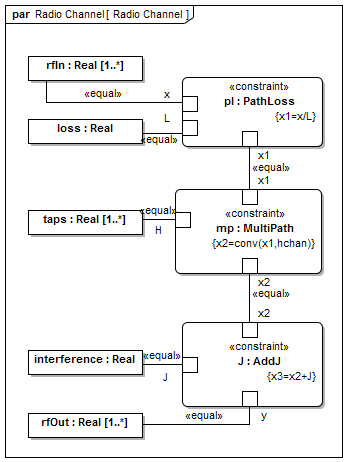
\includegraphics[width=0.6\textwidth]{./chapter-sysml/diagrams/par__Radio_Channel__Radio_Channel}%
	\caption{SysML parametric diagram of the radio channel constraints of the industrial wireless network.}%
	\label{sysml:fig:par:iwn-radio}
\end{figure} 

\paragraph{Data Constraints}\label{sysml:sec:constraints:data}

\begin{figure}[tbp]
	\centering
	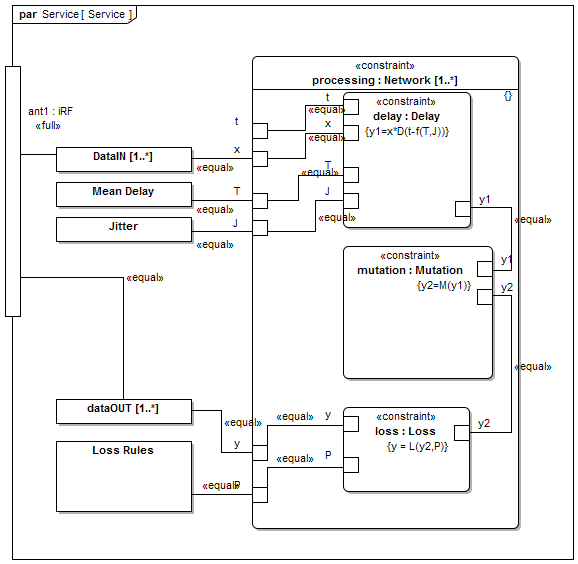
\includegraphics[width=0.8\columnwidth]{./chapter-sysml/diagrams/par__Service__Service}%
	\caption{SysML parametric diagram of the data constraints applied to the industrial wireless network.}%
	\label{sysml:fig:par:iwn:data}
\end{figure}    

Delay, mutation, and loss of information within the industrial wireless network are encapsulated by the Network constraints block.  The Network constraint is applied to wireless devices within the network and represents the impacts of the radio channel and network components and protocols.  These constraints are illustrated in a parametric diagram of Fig.~\ref{sysml:fig:par:iwn:data} in which the rules for delay, mutation, and loss are applied to a service of an industrial wireless network within a work-cell. As with any constraint, the rules for data loss may be modeled as equations, psuedocode, or executable computer code such as MATLAB script or C.  These rules decide if information is lost due to delay or mutation.  While it is easy to understand how mutation leads to loss through a mechanism such as a checksum, unacceptable delay can also lead to loss of data.  

% equations for data constraints
Delay is simply a function of time, the physical environment of the factory work-cell, and state of the network at time, $t$. Many features of the network and the physical environment will have an impact on the output of the delay equation and will include data transmission duration, radio wave propagation delay, signal-to-noise, protocol for reliability, routing, internal queuing, and processing. A generalized equation for information delay by the wireless network is given as the sum of processing delay, queuing delay, transmission delay, and propagation delay. Subsequently, information loss is modeled as a set of rules governed by the attributes of the network infrastructure, transport medium, and protocols shown in~\eqref{eq:network-loss}. These rules may include thresholds for unacceptable delay and the ability of the network to correct for data mutation or loss in the physical channel (i.e. the air interface).

\begin{equation}\label{eq:network-loss}
\mathcal{Y}(t,\mathcal{X},\mathcal{N}) = 
\begin{cases} 
\mathcal{X} & \text{if } \mathcal{X} \vdash \mathcal{L}(t,\mathcal{X},\mathcal{N}) \\
\emptyset   & \text{otherwise}
\end{cases}
\end{equation}
where $\mathcal{X}$ and $\mathcal{Y}$ are blocks of data traversing the network and $\mathcal{N}$ is the state of the network at time, $t$.	We model the loss constraints as a general set of rules, $\mathcal{L}$, taking into account that each network system will have a different set of configuration attributes and protocols.  The rules will therefore change for each operational system and the networks used.  When the rules for loss are applied, the output of the network, $\mathcal{Y}$, becomes the input to the network, $\mathcal{X}$, when $\mathcal{X}$ satisfies $\mathcal{L}(t,\mathcal{X},\mathcal{N})$.

\subsection{Application}\label{sysml:sec:application}

\begin{figure}[tbp]
	\centering
	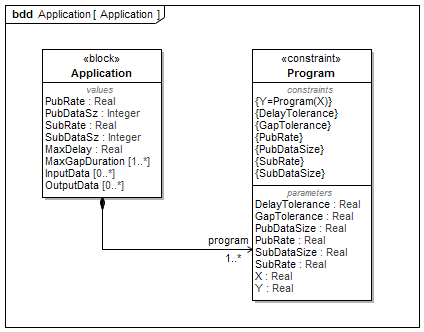
\includegraphics[width=0.8\columnwidth]{./chapter-sysml/diagrams/bdd__Application__Application}
	\caption{Block definition diagram of the Application.}
	\label{sysml:fig:application:bdd}
\end{figure}

Applications, commonly implemented as software and firm-ware, represent the intelligence of devices. The application defines the behavior and the information flow requirements of the work-cell~\cite{appWorkcell1996, appWorkcell2001, appWorkcell2011}.  As defined in the model, without Applications implemented in software, firmware, or hardware, the work-cell devices would not function.  The definition of the Application block is shown in Fig.~\ref{sysml:fig:application:bdd}.  The Application block is constrained by the Program constraint which defines the logic of the program, its expected data flow input rates, and its tolerances to delay and information loss.  Devices host multiple applications each with a unique set of constraint properties.  It is essential when constructing a work-cell model that each application is identified and modeled appropriately.  An example of an Application is a collision detection system within a robot controller. Table~\ref{tab:sample:constraints} illustrates sample parameters used in the collision detector Application.

% 	\vbox{%
% 		\begin{description}[align=left, labelindent=5mm]
% 			\label{sysml:fig:CollDet:example}
% 			\item [Program] Collision Detector
% 			\item [Constraints] ~
% 			\begin{description}[align=left]
% 				\item[Input Data] robot states, 1 KB
% 				\item[Subscription Rate] robot states, 125 \si{\Hz}
% 				\item[Max Delay Tol.] robot states, 47 \si{\us}
% 				\item[Max Loss Duration] robot states, 275 \si{\ms}
% 			\end{description}
% 		\end{description}
% 	}

\begin{table}[tbp]
	\centering
	\caption{Constraints Pertaining to a Collision Detector} \label{tab:sample:constraints}
	% Table generated by Excel2LaTeX from sheet 'constraints'
	\begin{tabular}{lc}
		
		\textbf{Constraint Property} &
		\textbf{Typical Value}
		\\
		\midrule
		Input Payload Size &
		1 KB
		\\
		Subscription rate &
		125 Hz
		\\
		Maximum Delay Tolerance &
		47 $\mu$s
		\\
		Maximum Loss Duration &
		275 ms
		\\
	\end{tabular}%
	
\end{table}

Specification of Application constraints provides a clear picture of the requirements of the factory automation system which can be projected on the wireless network. Through this process, it is possible to determine such requirements as scalability, throughput, reliability, and latency of the supporting network services modeled as radio and data constraints in Section~\ref{sysml:sec:general:constraints}. Indeed, as the manufacturing system becomes more complex and wireless becomes essential to communication, the projection of manufacturing requirements onto the wireless communication system becomes less clear.  Frequency planning, transmission scheduling, and error correction schemes become less obvious, and considerations of power, reliability, latency, and scale become optimization trade-offs. Such analyses are not within the scope of this paper but are important considerations for future research of manufacturing systems.  As such, the architectural elements and information flows exposed by an abstract model are a necessary first step.

\subsection{Industrial Wireless Network}

Central to the automation system is connectivity among devices and controllers~\cite{controlWSAN2010}.  More specifically, modern automation systems often employ networks to conduct inter-device communication~\cite{wirelessAutomation2017}.  The term \textit{inter-device} is appropriate as the Device block serves as the basis for all other components that communicate through the network.  Our model of the IWN is composed simply as a radio channel, a set of services, and a set of clocks as shown in Fig.~\ref{sysml:fig:iwn:bdd}.  This simplification of the model is necessary to allow the users of the model to provide as much or as little detail of the implementations of the radio channel and underlying services as required for their implementations.

%\begin{figure}[tbp]
%	\centering
%	\subfloat[\label{sysml:fig:iwn:bdd}]{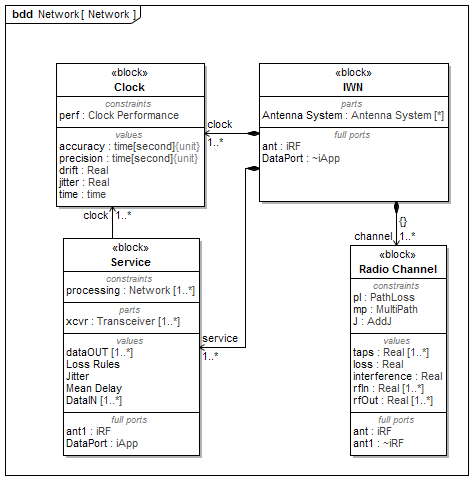
\includegraphics[width=0.99\columnwidth]{./chapter-sysml/diagrams/bdd__Network__Network}}
%	\hfill
%	\subfloat[\label{sysml:fig:iwn:ibd}]
%	{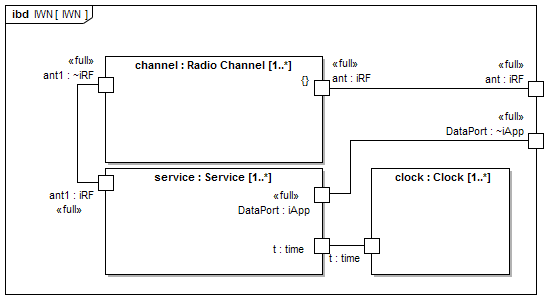
\includegraphics[width=0.99\columnwidth]{./chapter-sysml/diagrams/ibd__IWN__IWN}}
%	\hfill
%	\subfloat[\label{sysml:fig:iwn-services:ibd}]
%	{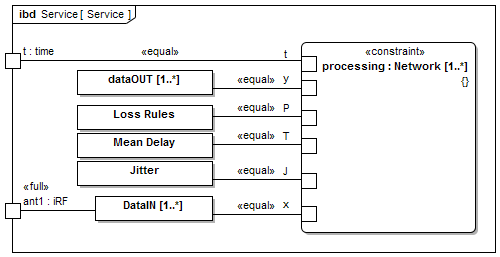
\includegraphics[width=0.99\columnwidth]{./chapter-sysml/diagrams/ibd__Service__Service}}\\
%	\caption{The BDD~\protect\subref{sysml:fig:iwn:bdd} and IBD~\protect\subref{sysml:fig:iwn:ibd} of the industrial wireless network with parametric IBD~\protect\subref{sysml:fig:iwn-services:ibd} of the Services block.}
%	\label{sysml:fig:iwn:ibd:full}
%\end{figure}

\begin{figure}[ht]
	
	\centering
	
	\begin{subfigure}{.8\textwidth}
		\centering
		% include first image
		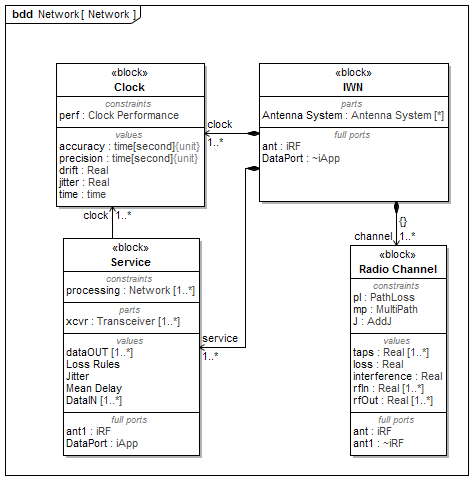
\includegraphics[width=.8\linewidth]{./chapter-sysml/diagrams/bdd__Network__Network}  
		\caption{Put your sub-caption here}
		\label{sysml:fig:iwn:bdd}
	\end{subfigure}

	\begin{subfigure}{.8\textwidth}
		\centering
		% include second image
		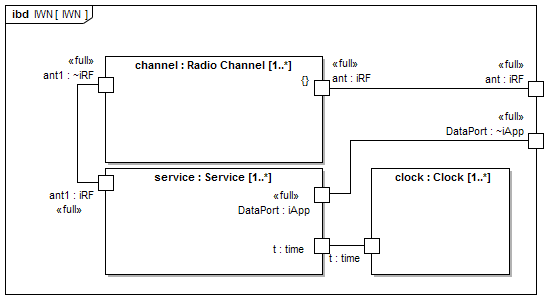
\includegraphics[width=.8\linewidth]{./chapter-sysml/diagrams/ibd__IWN__IWN}  
		\caption{Put your sub-caption here}
		\label{sysml:fig:iwn:ibd}
	\end{subfigure}

	\begin{subfigure}{.8\textwidth}
	\centering
	% include second image
	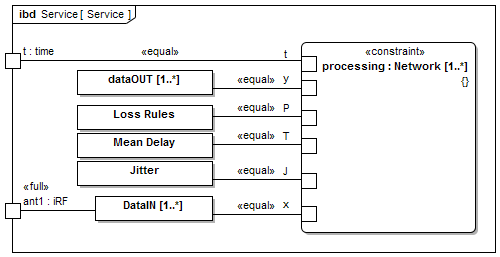
\includegraphics[width=.8\linewidth]{./chapter-sysml/diagrams/ibd__Service__Service}  
	\caption{Put your sub-caption here}
	\label{sysml:fig:iwn-services:ibd}
	\end{subfigure}

	\caption{The BDD~\protect\subref{sysml:fig:iwn:bdd} and IBD~\protect\subref{sysml:fig:iwn:ibd} of the industrial wireless network with parametric IBD~\protect\subref{sysml:fig:iwn-services:ibd} of the Services block.}
	\label{sysml:fig:iwn:ibd:full}
\end{figure}

Connectivity of a constructed IWN is shown in Fig.~\ref{sysml:fig:iwn:ibd}.  An IWN is internally modeled such that information flows as radio frequency (RF) energy through the \textit{ant} port.  A radio channel is applied, theoretically for each pairwise link, and the modified signal is passed to the services for processing.  Network processing is modeled by the properties of network constraints as defined in Section~\ref{sysml:sec:constraints:data}.  Once processed by network services, information is routed back through the radio channel through the \textit{ant} port to other Devices connected to the IWN.  Moreover, the Service block includes a parametric model as shown in Fig.~\ref{sysml:fig:iwn:ibd:full}. This IBD with exposed parametrics exemplifies the inclusion parameters such as information delay and loss caused by the IWN, but it also exemplifies the impact of protocols and infrastructure (throughput, memory, etc.) within the network.  These effects are modeled as rules of loss shown in~\eqref{eq:network-loss}.

\subsection{Devices}\label{sysml:sec:devices}

\subsubsection{Device}\label{sysml:sec:devices:device}

A Device, defined in Fig.~\ref{sysml:fig:bdd:devices}, is generic construct representing an element within the work-cell with processing, memory, and storage capability. Devices have the capability to run applications as defined in Section~\ref{sysml:sec:application}.  Devices are sub-classed into Sensor and Actuator devices which generically refer to any type of sensor or actuator, and, in particular, the wired variety.  The Device is further sub-classed to the Wireless Device which is the central theme of our analysis.  Derived from the Wired Device are the Wireless Sensor and Wireless Actuator as well as the Controller.  The Controller represents the base class for deriving work-cell devices such as the PLC and the Robot Controller, sections~\ref{sysml:sec:plc} and~\ref{sysml:sec:robotics}, respectively, and provides support for external input-output (IO).

\begin{figure}[H]
	\centering
	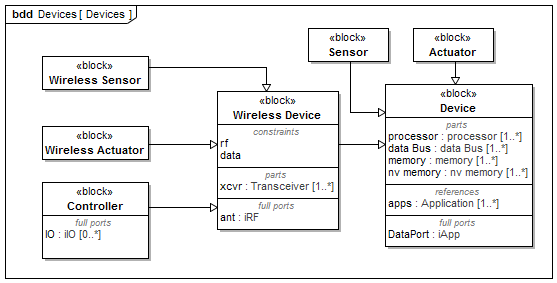
\includegraphics[width=0.95\columnwidth]{./chapter-sysml/diagrams/bdd__Devices__Devices}%
	\caption{SysML block definition diagram of wireless devices within the factory work-cell.}%
	\label{sysml:fig:bdd:devices}
\end{figure}



\subsubsection{Wireless Devices}\label{sysml:sec:devices:wireless-device} 
A Wireless Device is a subclass of Device that contains the various components necessary for untethered communication.  These devices then communicate with each other through one or more industrial wireless networks (IWNs) which contains antenna systems, transceivers, protocols, and network services.  The relationships and composition of the Wireless Device are illustrated in Fig.~\ref{sysml:fig:wirelessdevice:full}. As shown, the wireless device is composed of at least one transceiver and each transceiver is composed of at least one antenna system which is composed of at least one antenna element.  The antenna system is constrained by its gain profile.

%\begin{figure}[tbp]
%	\centering
%	\subfloat[Block definition diagram of the Wireless Device\label{sysml:fig:wirelessdevice:bdd}]{%
%		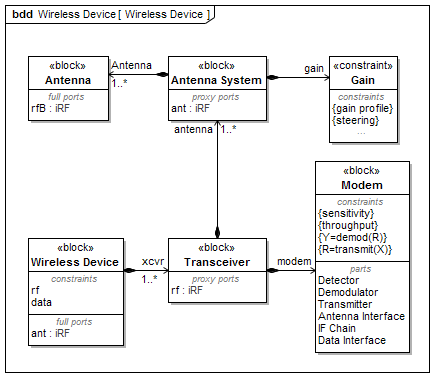
\includegraphics[width=0.95\columnwidth]{./chapter-sysml/diagrams/bdd__Wireless_Device__Wireless_Device}
%	}
%	\hfill
%	\subfloat[Internal block diagram of the Wireless Device\label{sysml:fig:wirelessdevice:ibd}]{%
%		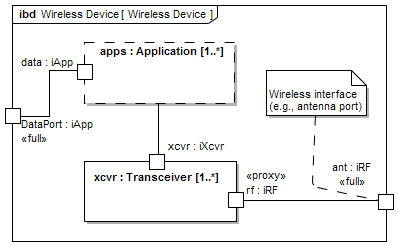
\includegraphics[width=0.95\columnwidth]{./chapter-sysml/diagrams/ibd__Wireless_Device__Wireless_Device}
%	}  
%	\caption{Block definition diagram~\protect\subref{sysml:fig:wirelessdevice:bdd} and the internal block diagram~\protect\subref{sysml:fig:wirelessdevice:ibd} of Wireless Device.}
%	\label{sysml:fig:wirelessdevice:full}      
%\end{figure}

\begin{figure}[ht]
	\centering
	
	\begin{subfigure}{.8\textwidth}
		\centering
		% include first image
		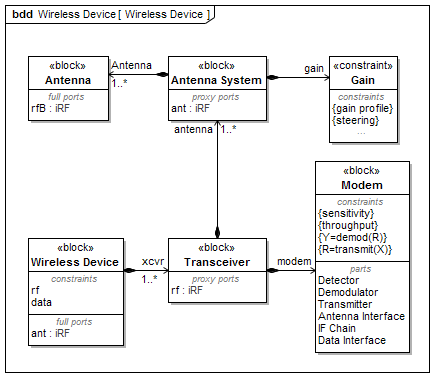
\includegraphics[width=.95\linewidth]{./chapter-sysml/diagrams/bdd__Wireless_Device__Wireless_Device}  
		\caption{Block definition diagram of the Wireless Device}
		\label{sysml:fig:wirelessdevice:bdd}
	\end{subfigure} 

	\begin{subfigure}{.8\textwidth}
		\centering
		% include second image
		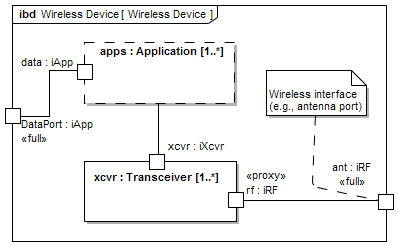
\includegraphics[width=.95\linewidth]{./chapter-sysml/diagrams/ibd__Wireless_Device__Wireless_Device}  
		\caption{Internal block diagram of the Wireless Device}
		\label{sysml:fig:wirelessdevice:ibd}
	\end{subfigure}

	\caption{Block definition diagram~\protect\subref{sysml:fig:wirelessdevice:bdd} and the internal block diagram~\protect\subref{sysml:fig:wirelessdevice:ibd} of Wireless Device.}
	\label{sysml:fig:wirelessdevice:full}
\end{figure}

\subsubsection{Test Device}\label{sysml:sec:test-device}

%\begin{figure}[tbp]
%	\centering
%	\subfloat[Block definition diagram of the Test Device\label{sysml:fig:testdevice:bdd}]{%
%		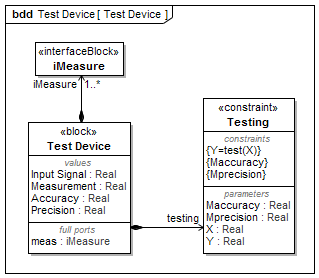
\includegraphics[width=0.95\columnwidth]{./chapter-sysml/diagrams/bdd__Test_Device__Test_Device}
%	}
%	\hfill
%	\subfloat[Internal block diagram of the Test Device\label{sysml:fig:testdevice:ibd}]{%
%		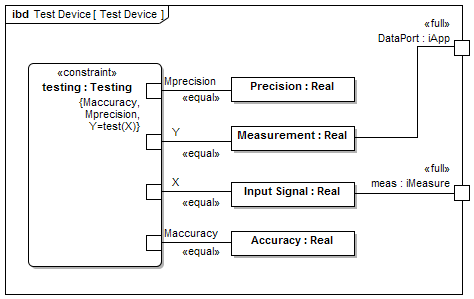
\includegraphics[width=0.95\columnwidth]{./chapter-sysml/diagrams/ibd__Test_Device__Test_Device}
%	}  
%	\caption{Block definition diagram~\protect\subref{sysml:fig:testdevice:bdd} and the internal block diagram~\protect\subref{sysml:fig:testdevice:ibd} of Test Device.}
%	\label{sysml:fig:testdevice:full}      
%\end{figure}

\begin{figure}[ht]
	
	\centering
	
	\begin{subfigure}{.8\textwidth}
		\centering
		% include first image
		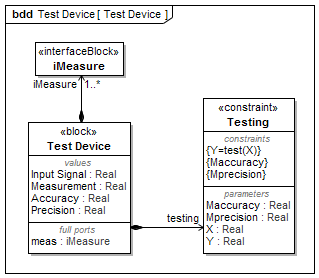
\includegraphics[width=.95\linewidth]{./chapter-sysml/diagrams/bdd__Test_Device__Test_Device}  
		\caption{Block definition diagram of the Test Device}
		\label{sysml:fig:testdevice:bdd}
	\end{subfigure}

	\begin{subfigure}{.8\textwidth}
		\centering
		% include second image
		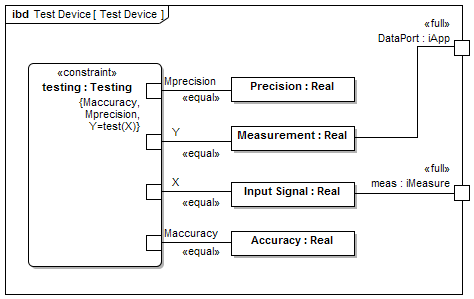
\includegraphics[width=.95\linewidth]{./chapter-sysml/diagrams/ibd__Test_Device__Test_Device}  
		\caption{Internal block diagram of the Test Device}
		\label{sysml:fig:testdevice:ibd}
	\end{subfigure}

	\caption{PBlock definition diagram~\protect\subref{sysml:fig:testdevice:bdd} and the internal block diagram~\protect\subref{sysml:fig:testdevice:ibd} of Test Device.}
	\label{sysml:fig:testdevice:full}
	
\end{figure}

The Test Device is a subclass of Device that represents devices used for calibration or ground truth testing of properties of a work-cell.  The block definition and internal configuration are illustrated in Fig.~\ref{sysml:fig:testdevice:full}.  A Test Device is constrained by its accuracy and precision as well as the algorithm for controlling measurement.  An example of a test device is a calibrated force sensor that may be used as comparison to a 6-DOF wireless sensor mounted on the wrist of a robot arm as shown in the top left of Fig.~\ref{sysml:fig:workcell:examples}. Test devices are useful and necessary elements of the wireless testbed to establish accurate and repeatable ground truth measurements.  For example, a stationary precision force sensor may be used to establish a ground truth force value, and a high-accuracy vision tracking system is used for truth in position.  Test devices are modeled such that measurements may traverse the operational wireless network or a stand-alone wired interface.

\subsection{Robotics}\label{sysml:sec:robotics}

%\begin{figure}[tbp]
%	\centering
%	\subfloat[Block definition diagram of the Robot Controller\label{sysml:fig:robotcontroller:bdd}]{%
%		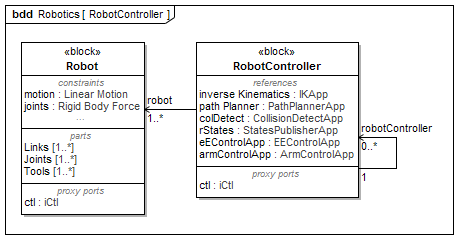
\includegraphics[width=0.5\columnwidth]{./chapter-sysml/diagrams/bdd__Robotics__RobotController}
%	}
%	\hfill
%	\subfloat[Internal block diagram of the Robot Controller\label{sysml:fig:robotcontroller:ibd}]{%
%		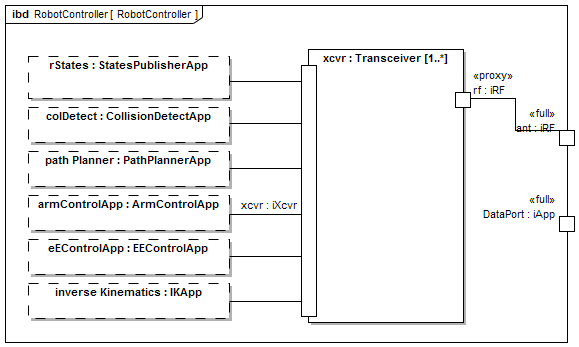
\includegraphics[width=0.5\columnwidth]{./chapter-sysml/diagrams/ibd__RobotController__RobotController}
%	}  
%	\caption{The BDD~\protect\subref{sysml:fig:robotcontroller:bdd}, IBD~\protect\subref{sysml:fig:robotcontroller:ibd} of the Robot Controller.}
%	\label{c}	
%\end{figure}

\begin{figure}[ht]
	
	\centering
	
	\begin{subfigure}{.5\textwidth}
		\centering
		% include first image
		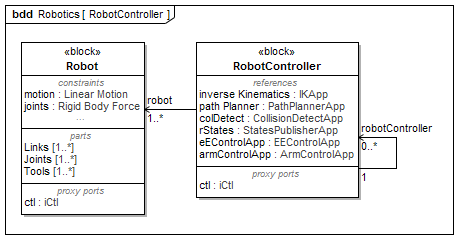
\includegraphics[width=.8\linewidth]{./chapter-sysml/diagrams/bdd__Robotics__RobotController}  
		\caption{Block definition diagram of the Robot Controller}
		\label{sysml:fig:robotcontroller:bdd}
	\end{subfigure}

	\begin{subfigure}{.5\textwidth}
		\centering
		% include second image
		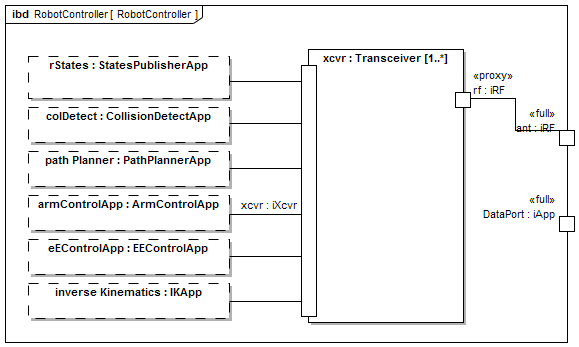
\includegraphics[width=.8\linewidth]{./chapter-sysml/diagrams/ibd__RobotController__RobotController}  
		\caption{Internal block diagram of the Robot Controller}
		\label{sysml:fig:robotcontroller:ibd}
	\end{subfigure}

	\caption{The BDD~\protect\subref{sysml:fig:robotcontroller:bdd}, IBD~\protect\subref{sysml:fig:robotcontroller:ibd} of the Robot Controller.}
	\label{sysml:fig:robotcontroller:full}
	
\end{figure}

The robotics package contains elements specific to robot systems.  Robot systems are composed of at least one robot controller associated with one or more robots, as shown in Fig.~\ref{sysml:fig:robotcontroller:bdd}.  In manufacturing, robots interact with their surrounding to accomplish assigned tasks such as tending machinery, moving materials, welding, and inspecting. Robot controllers provide support for external IO devices.  In addition, modern robot controllers will support a variety of open and proprietary network protocols allowing for interaction with other actors in the work-cell.  The robot controller's main task is control of the rigid body dynamics of the robots which is usually conducted via real-time communication over a high-throughput serial field-bus. While joint control is conducted using wires, the robot controller is responsible for other tasks requiring reliable, low-latency communication in which wireless may serve a role.  These tasks are captured in the model as applications (Fig.~\ref{sysml:fig:robotcontroller:ibd}) and explained as follows.

\begin{description}
	
	\item[\textbf{Robot States Publisher}] Transmission of robot states to external actors such as other robot controllers, supervisors, and safety systems.
	
	\item[\textbf{Arm Controller}] Also known as manipulator control, serves to accept position commands as Cartesian or joint space trajectories and waypoints from other actors within the work-cell.
	
	\item[\textbf{End Effector Control}] Command and control of the robot end-effector such as a gripper or sensor.  The end-effector may be equipped with a high-throughput wireless sensor necessitating reliable communication.
	
	\item[\textbf{Inverse Kinematics}] Converts Cartesian coordinates of the end-effector into joint positions.
	
	\item[\textbf{Path Planner}] Determines the optimal geometrical trajectory to achieve a final pose given knowledge of self-collision and real-time knowledge of the surround environment.  Path planning is a sophisticated part of a robot system and may be allocated to an external system depending on throughput and latency requirements.
	
	\item[\textbf{Collision Detector}] This application monitors the states of other actors and obstructions within the work-cell. If possibility of collision is detected, the collision detector takes action.
	
\end{description} 

These applications within the robotic work-cell define many information flows requiring careful analysis to achieve reliability and latency necessary for the safety and control of the manufacturing process. Information flows are identified in Section~\ref{sysml:sec:wireless-infoflows}.

\subsection{PLC}\label{sysml:sec:plc}
The PLC is a specialized class of Controller.  PLCs were originally developed to mirror relay circuits in software; however, the modern PLC is much more advanced and is usually equipped with multiple processors, a real-time operating system (OS), and capabilities to support various types of industrial IO devices.  In addition, modern PLCs (also called automation servers) include both a general purpose OS with a real-time kernel and multiple network interfaces.  Many network-routable protocols are also supported.  With the addition of wireless protocols, PLCs now have the ability to support IO devices connected remotely without wires.  Supervision of untethered robots is also possible using PLCs.  The PLC is modeled as a Controller device with the work-cell model.  Shown in Fig.~\ref{sysml:fig:PLC:ibd}, the PLC is modeled as a wireless device with transceiver, logic application, and safety applications.  More sophisticated PLCs may be modeled by extending the PLC block.  As applications, the logic and safety functions are constrained by application constraints. Finally, as Controller devices, PLCs are modeled with an IO port, thus IO can be connected to the PLC by wires or by wireless network connection.

\begin{figure}
	\centering
	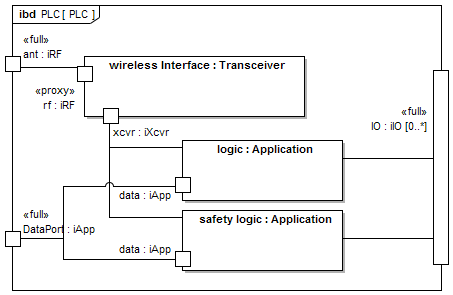
\includegraphics[width=0.95\columnwidth]{./chapter-sysml/diagrams/ibd__PLC__PLC}
	\caption{The IBD of the PLC showing composition and connectivity of the control logic and safety logic Application instantiations to the Transceiver interface. }
	\label{sysml:fig:PLC:ibd}
\end{figure}

\subsection{Safety}\label{sysml:sec:safety}
% 	\textcolor{red}{MOHAMED TO WRITE}
% 	\textcolor{blue}{Allocation of safety features from the PLC. High availability IO input devices, output relays, used for E-STOP usually to protect life and property; constrained by response time requirement of the safety rating}

In a work-cell with interacting humans and robots, functional safety requirements are typically strict by specifying the rules related to four main safety criteria, namely, monitored stops, controlled speeds, separation distances, and power and force limits in order to prevent injury for humans and damage for equipment. The wireless safety package is composed of a safety controller and safety devices. Traditionally, the safety requirements of the work-cell is fixed and managed by the safety controller which receives safety-related measurements and takes the corresponding actions. Alternatively, the safety controller may be connected to the PLC where the current work-cell activities are supervised.  The PLC will determine the required safety rating and the safety controller behaves accordingly. The dedicated safety controller is needed to achieve the required high reliability and low latency safety requirements and it can be a general PLC with safety modules. 

The safety devices include non-safety-rated devices such as the various work-cell sensors and actuators and safety-rated input and output devices. Safety control input devices include Emergency-stop and enabling buttons while output devices include relays and switches for various work-cell equipment. The use of wireless in safety control loops allows installing a larger number of sensing devices including vision systems to monitor the human and robots activities, velocity and proximity sensors, and machine status sensors. Moreover, wireless allows to have mobile control panels where workers can activate a safety device at any time and location within the work-cell.        

\subsection{Vision}\label{sysml:sec:vision}
% 	\textcolor{red}{MOHAMED TO WRITE}
% 	\textcolor{blue}{composition (vision processing, optical devices with networking interfaces, general panning and zooming, object detection, interface to robotic system, interface to the supervisory system)}

%     \textcolor{green}{Make that we allow the following in your definition: part tracking, object detection, intput to collision avoidance systems, tracking of mobile robots, augmented reality devices/systems, security cameras, etc.}
The vision system considered in this subsection is the one used for work-cell monitoring and general object detection. It does not cover the machine-embedded vision systems which can be used for inspection and characterization of objects such as the shape, color, texture, or size of processed materials. The data collected by the work-cell vision system can be used for parts and mobile robots tracking, collision avoidance, object detection, security identification systems, and augmented reality devices and systems. The vision system communicates with the supervisory control, robotic controller, and the safety system to provide the work-cell state which contains the positions of various equipment, robots, and humans. 

The vision system is composed of optical devices, vision processing unit, and interfaces to various work-cell systems. The optical devices are the cameras for capturing images at high enough speed to track and detect various objects. These cameras have wireless network interfaces to be connected to the vision processing unit to allow collaborative processing of the captured images and obtaining precise work-cell state. The vision processing unit performs data acquisition from the distributed optical devices and feature extraction to detect and track the positions of various entities in the work-cell. 

The vision system communicates the corresponding data to the supervisory control, robotic control, and the safety system for decision making based on the captured work-cell state. The supervisory controller uses vision system data for robots and workers localization, parts detection and identification, and schedules tasks using this information. The robotics controller uses these data for motion control, path planning, and collision detection. Finally, the safety controller uses these data for safety requirements implementation such as enforcing safety stops, controlling the speeds of moving objects, and limiting power and forces of various work-cell components.    

\subsection{Spectrum Monitoring System}\label{sysml:sec:sms}
A spectrum monitoring system (SMS) is an often overlooked yet valuable part of the wireless factory work-cell with requirements specified in~\cite{Candell2017.SMS}.  The SMS is modeled as an atomic agent within the work-cell.  The SMS Agent is one component in a larger enterprise-level spectrum monitoring deployment.  The SMS agent shown in Fig.~\ref{sysml:fig:sms:bdd} includes a transceiver, an event detector, and a reporting agent.  The transceiver can be implemented as an RF-to-baseband converter.  The detector application is responsible for detection and estimation of anomalous spectral events and may employ machine learning to accurately detect anomalies and report localized spectral events.

The reporter application collects, filters, and reports event information to a central management console.  SMS reports support identification of long-term patterns such as growth trends in particular wireless bands.  Since the SMS Agent is part of a larger network of spectrum monitoring, it is presumed that reports are wirelessly transmitted back to the enterprise management console.  These reporting events use bandwidth otherwise used for the factory operation, thus reports must be made concise and infrequent.  This implies substantial filtering and intelligence in the local SMS agents This may provide opportunities for research.

Detection events may be routed to the local supervisor, robot controller, and safety system.  By leveraging spectral awareness, work-cells can be made safer and more reliable.  As SMS are not yet widespread in industrial applications; thus, standardized protocols are needed for reporting and integration with automation systems.

\begin{figure}[tbp]
	\centering
	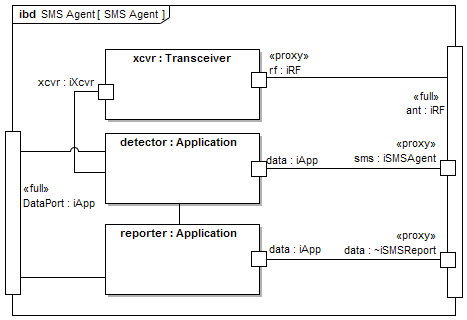
\includegraphics[width=0.99\columnwidth]{./chapter-sysml/diagrams/ibd__SMS_Agent__SMS_Agent}
	\caption{Spectrum monitoring agent composed of transceiver, detection application, and reporting application.}
	\label{sysml:fig:sms:bdd}
\end{figure}

\subsection{Human}\label{sysml:sec:human}
% 	\textcolor{red}{Mohamed to write}
% 	\textcolor{blue}{People; wearable devices such as gas sensors, identification, and localization; could be security related for access control; portable devices; personal devices; include motion on factory floor; operational tasks; intervention of process      
% 		Composition, constraints of motion}

Humans can exist in a modern work-cell for short or long periods of time depending on the required task. Two categories of human-related aspects are captured in the work-cell model. First, the human existence in the work-cell leads to detection and identification of the corresponding worker for both safety and security. Also, human motion within the work-cell requires position tracking for environment monitoring and spectrum monitoring due to radio frequency channel variations with human movements. The second category includes the human interfaces with the work-cell process that include portable control devices, wearable sensors, and workers communication devices to get task commands. Moreover, depending on the process constraint, personal devices of workers may interfere with the work-cell communications if allowed.      

\section{Results of a Work-cell Case Study}\label{sysml:sec:wireless-infoflows}
% Rick's section	
\begin{figure*}[tbp]
	\centering
	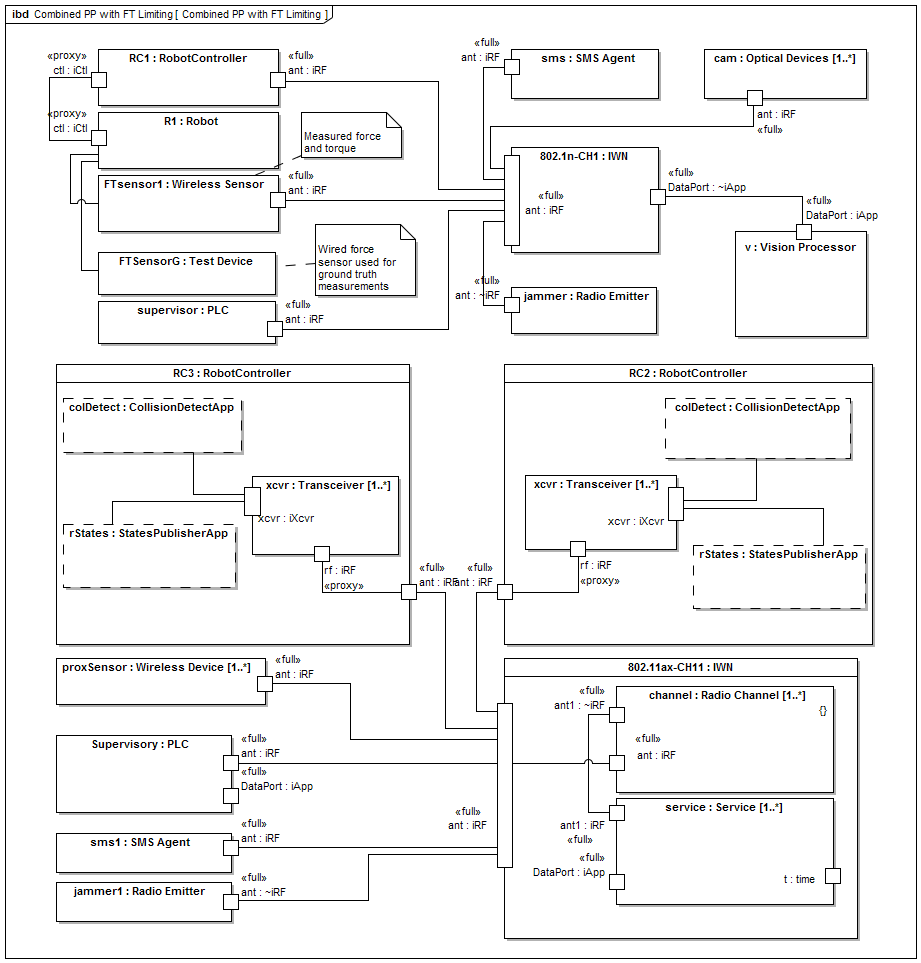
\includegraphics[width=0.95\textwidth]{./chapter-sysml/diagrams/ibd__Combined_PP_with_FT_Limiting__Combined_PP_with_FT_Limiting}
	\caption{IBD of a work-cell employing multiple networks in collaborative robot operation coexisting with robot force limiting inspection station.}
	\label{sysml:fig:workcell:examples}     
\end{figure*}

In this section we present a case study of a work-cell which includes a force-torque limiter robot application and a two-robot collaborative pick and place operation.  The model for this system is depicted in Fig.~\ref{sysml:fig:workcell:examples}.  The number and type of wireless information flows will depend on the configuration of the work, the number of applications, and the places where wireless is applied. For this case study, the force limiter section is composed of a robot controller, a robot, and an FT sensor. A PLC is used for work-cell supervision, and a test device is deployed for ground truth measurement.  An SMS agent monitors the electromagnetic spectrum.  A Radio Emitter is included to model the transmission of interference.  An IEEE 802.11n network is represented in the model by an IWN block. Properties of the radio channel and services of the communication system are therefore represented. Similarly, another example is implemented in \cite{SysML.Candell2018} for a pick-and-place scenario where the model is composed of two robots, a PLC, an IWN, and an SMS Agent in addition to proximity sensors and an IEEE 802.11ax network.

Referring to these examples, typical information flows are easily identified as connections between Wireless Device blocks and the antenna port, \textit{ant}, of the IWN.  Recall that the IWN includes radio channel and services offered by the network itself.  Therefore, all wireless information flows will traverse the IWN through the \textit{ant} port.  Applications are implied and produce and consume the information according to associated constraint properties.  Information flows are generated by the interactions between actors and include the following:  

\begin{description}
	
	\item[\textbf{Robot States}] The geometry states of the robot such as position, velocity, and acceleration of each joint or end-effector. Robot states may include Cartesian or joint space readings depending on the need of other applications or the capabilities of publisher.  Robot states are usually transmitted at 30 Hz or faster~\cite{JMarvel2017}.
	
	\item[\textbf{Force Sensor Readings}] The readings from a sensor mounted on the wrist of each robot arm. These readings are typically in the format of wrenches (linear and angular forces) and are transmitted at rates from 15 Hz for monitoring applications up to 500 Hz for force limiting and control applications~\cite{onrobot}. Other sensors may produce data in the system such as proximity sensors which can generate data in the range of 1-50 Hz~\cite{DiffuseSensorSpecs} and Tactile sensors which can have information flow rates faster than 1000 Hz~\cite{TactileInternet}.
	
	\item[\textbf{Machine Health Monitoring}] Readings from sensors mounted within machinery such as mills, routers, and lathes used to sense and predict deviations of mechanical components from design tolerances. Readings for prognostics and health monitoring are often aggregated at the source with statistical metrics being communicated to a factory enterprise application; however, non-aggregated readings may also be transmitted to a remote signal analyzer.  Health monitoring sensors measure temperature, vibration, acceleration, inclination, position, and rates of change of angles. Information flows from a single aggregation point may reach 200 kB/s on average for a 6-DOF sensor apparatus described in~\cite{ELWeiss}. While the outputs of health monitoring sensors are usually wired into a local aggregation devices, it is desirable to transmit these readings to an on-line optimizer or PLC within the work-cell~\cite{Weiss2016.PHM}.
	
	\item[\textbf{IO States and Supervisory Messages}] These contain both the boolean-valued readings and commands from sensors, and task orders in the form of short commands and lists of instructions which can originate from any supervisor within the network such as a PLC or other controller. Sensor readings (inputs) and actuation commands (outputs) are transmitted in periodically or pseudo-randomly at rates indicative of movements of machinery and materials through the manufacturing process.  Typical analog and boolean IO states range from to 10 Hz to 100 Hz depending on the manufacturing process~\cite{TwinCAT}.
	% 		\item[Supervisory Messages] Directives and task orders in the form of short commands and lists of instructions and can originate from any supervisor within the network such as a PLC or other controller. Supervisory messages include state information such as task status from collaborating actors within the work-cell. 
	
	\item[\textbf{SMS Events}] The SMS agent will communicate state information and directives to controllers within the work-cell.  These messages allow the automation system to react under anomalous spectrum conditions within the work-cell. These information flows may be necessary for safe operation of the work-cell. The data rate of reports from an SMS agent without processing or compression can be in the range of 1 to 10 megabits per second (Mbps)~\cite{cuevas_2015}.
	
	\item[\textbf{Vision Applications}] The vision system will communicate videos or images for processing and decision making. Typical Video flows can have the rates of 30 Hz for surveillance and 125 Hz for motion capturing~\cite{industrialCCTV, ELWeiss}. Information flow for Object tracking systems can have the rate of 10-200 Hz depending on the tracked objects and the required accuracy~\cite{lidar, motioncapture}. 
\end{description}
%\vspace{5mm}


%     % THIS TABLE TO BE REMOVED 8/2/2018
% 	\begin{table}[tbp]
% 		\centering
% 		\caption{Work-cell information flows.}
% 		\label{tab:infoflows}
% 		\begin{threeparttable}
% 			%begin tabular
% 			% Table generated by Excel2LaTeX from sheet 'infoflows (2)'
\begin{tabular}{lccc}
\textbf{Information Flow} &
  \textbf{Information Rate (Hz)} &
  \textbf{Protocol} &
  \textbf{Citation}
  \\
\midrule
\textbf{Robotics} &
   &
    &
  
  \\
Joint states &
  30-1000 &
  Datagram &
  \cite{JMarvel2017}
  \\
Task states &
  1-5 &
  Reliable &
  TBS
  \\
End-effector commands &
  \tnote{*} &
  Reliable &
  TBS
  \\
Collision events &
  \tnote{*} &
  Reliable &
  TBS
  \\
\midrule
\textbf{Sensors} &
   &
    &
  
  \\
Force/Torque &
  15-500 &
  Datagram &
  TBS
  \\
Proximity &
  1-50 &
  Reliable &
  \cite{DiffuseSensorSpecs}
  \\
Tactile &
  $>$1000 &
  Reliable &
  \cite{TactileInternet}
  \\
\midrule
\textbf{Vision} &
   &
    &
  
  \\
Video &
  30 (Surveillance)-175 (motion capture) &
  Datagram &
  \cite{industrialCCTV, labOpticalCameraSpecs}
  \\
Tracking &
  10-100 &
  Datagram &
  \cite{LIDA15Hz}
  \\
\midrule
\textbf{Supervision} &
   &
   &
  
  \\
Command/control &
  1-5 &
  Reliable &
  TBS
  \\
IO States &
  10-100 &
  Reliable &
  \cite{TwinCAT}
  \\
\midrule
\textbf{Spectrum Monitoring} &
   &
   &
  
  \\
SMS Events &
  \tnote{*} &
  Reliable &
  TBS
  \\
SMS Reports &
  <1 &
  Reliable &
  TBS
  \\
\bottomrule
\end{tabular}%
%end tabular
% 			\begin{tablenotes}
%             	\item[] \textcolor{blue}{add information about the purpose of this table. What are the flow items, impact to bandwidth, and }
% 				\item[*] Indeterminate flow rate
% 				\item[] \textcolor{red}{need validation and citations}
% 			\end{tablenotes}
% 		\end{threeparttable}
% 	\end{table}

\section{Discussion and Conclusions}\label{sysml:sec:conclusion}
A model was developed using SysML. The developed model is constructed of the elements necessary to construct useful representations of factory work-cells in which wireless networks are used to transport information necessary for automated control system operation.  Reusable, derivable elements are developed and then extended to represent the constructs of the work-cell such as robot control, supervisory control, vision, safety, and spectrum monitoring.  An industrial wireless network is then developed and constraints of the radio channel and network services are formalized. Using the architectural model, information flows are explored and incorporated within. 

It is important to mention that this model includes an often overlooked component of any industrial wireless deployment which is the spectrum monitoring system and also considers the human-robot and robot-robot interactions in industrial environments. The current model includes various systems constraints including motion constraints, radio channel constraints, and networking constraints. The parametric constraints are provided as examples and can be replaced with executable computer code thereby making the model useful for simulation depending on the modeling tool selected. Furthermore, the applications within the robotic work-cell define many information flows requiring careful analysis to achieve reliability and latency necessary for the safety and control of the manufacturing process.

With increased dependency on wireless communications for more complex manufacturing systems, the projection of manufacturing requirements onto the wireless communication system becomes less obvious. Such analysis of this projection is essential for future research of manufacturing systems. As such, the architectural elements and information flows exposed by an abstract model
are a necessary first step. Our model in its current state of development is comprehensive enough to support architectural and ontological analyses of the factory work-cell.  As such, information about the relationships between components of a work-cell and attributes related to the wireless network may be discovered. Therefore, our model serves as a foundation for future systems engineering analyses. Moreover, our model may be used as a tool for academic and industry exploration of wireless testbed development.  We make the model openly available through GitHub at~\cite{SysML.Candell2018}.

%% Link the GENERAL bibliogaphy to a BibTeX file.
%\bibliography{./chapter-sysml/bibsysml}
%\bibliography{bibliography}


\chapter{Application of Graph Databases}\label{chapter:graphdb}

\chapterintro*

The workcell is considered a main building block of various industrial settings. Hence, it is examined as a primary testing environment for studying wireless communication techniques in factory automation processes. A new testbed was recently designed and developed to facilitate such studies in workcells by replicating various data flows in an emulated production environment. In this paper, an approach to storing and analyzing network performance data from a manufacturing factory workcell is introduced.  A robotic testbed was constructed using two collaborative grade robot arms, machine emulators, and wireless communication devices. A graph database approach was implemented to capture network and operational event data among the components within the testbed.  A schema is proposed, developed, and elaborated; a database is then populated with events from the testbed, and the resulting graph is presented. Query commands are then presented as a means to examine and analyze network performance and relationships within the components of the network.  Additionally, this work demonstrates how to extract correlations between receive signal power and network delay within the testbed using the graph database query language.  Finally, using the inherently interconnected nature of the graph database, the works demonstrates how one might apply the graph database approach toward examining more complex relationships between the wireless communications network and the operational system.

\section{Introduction} \label{gdbappl:sec::intro}

% conceptual clarification
Wireless communication is a key enabling technology for the modernization of factory workcells. Modern factory workcells are highly-interconnected networked control systems in which various devices interact and collaborate to accomplish complex and adaptive production orders. The workcell often contains mobile robots that collaborate with other robots or human beings. Requirements of the workcell include the incorporation of mobile collaborative robotics with real-time coordination of motion and tool actuation.  As such, the communication of sensor and control information must be ultra-reliable and of low-latency to assure trustworthy operation~\cite{wirelessAutomation2017}. Due to an increased demand for ease of installation, reduced costs of deployment and maintenance, and flexibility, wired networks are being gradually replaced with wireless networks. This presents a real challenge for networks and control systems. Compared with wired connections, wireless links have their unique advantages in connecting field sensors and actuators with reduced cabling costs and natural support of mobility~\cite{ieMag2018}; however, most current communications systems lack the latency and reliability supports~\cite{etsi103588} mandated by factory owners~\cite{Industry40, SmartManuf}.  New wireless protocols are being designed to address reliability and latency concerns of real-time systems such as those in manufacturing automation.  These new protocols include advancements, such as the Institute of Electrical and Electronics Engineers (IEEE) 802.11ax standard and 5G cellular evolution as defined by the International Mobile Telecommunications-2020 (IMT-2020) Standard.  Both of these two standards employ improved diversity techniques for multiple access of devices as well as 1 ms latency and greatly improved reliability~\cite{80211ax}. 

Evaluation of such systems used in manufacturing environments requires not only rigorously analyzing  network performance, but also studying the impacts of networks on manufacturing systems. Additionally, industry lacks effective and easy-to-use strategies for test and evaluation of such systems in a way that correlates network performance with operational performance. Furthermore, since factory operators desire the ability to control operations within the workcell using wireless technology, the work presents a novel method to simultaneously capture network and operational event information using a graph database (GDB).  The use of a GDB allows for more intuitive inferences to be made through the stored relationships and graph theoretic models~\cite{Angles:2008:SGD:1322432.1322433}. In this paper, a GDB approach to the capture and analysis of factory workcell performance utilizing the Neo4j database platform is presented. A proposed schema of the database, the process for capturing both network and operational events, and examples of querying the database for cyber-physical performance evaluation of the workcell for the collaborative two-robot machine-tending workcell\cite{Liu2019vancouver} are provided.

\section{Related Work}
Previous work related to the application of graph databases was presented in the Chapter~\ref{chapter:soa} Section~\ref{chapter:soa:modeling}.

\section{Graph Databases}
A GDB is the type of databases that uses nodes, edges, and properties to store and present data. A GDB is a part of a family of databases known as NoSQL databases that are used often to represent complex interrelated structures of data and their relationships.  This can be very difficult with traditional relational databases.  The GDB places a high priority on the relationships (edges) between units of information.  In addition, the GDB does not enforce any particular schema or structure, and, therefore, provides greater flexibility in storing and representing information in which the parts of information may vary among units. The relationships within a GDB are efficiently queried because they are persistently stored within the database.  In a GDB, queries can be made based on relationships. This, in particular, presents an advantage when storing information regarding systems with correlations that are apparent but difficult to visualize or quantify. The GDB approach was chosen for this specific purpose\textemdash{}to quantify and visualize relationships between non-ideal communications within a workcell and their impact on the physical system.

%\section{Related Work}
%Multiple surveys about GDBs have been presented to describe the associated models, tools, and their features in~\cite{Angles:2008:SGD:1322432.1322433,7148480,GDB_overview}. Also, examples of applications and implementations of GDBs are presented in~\cite{modern_models} to show their use on enterprise data, social networks, and determining security and access rights. It was found that GDBs provide the much needed structure for storing data and incorporating a dynamic schema. On the other hand, query languages are used to extract data including traversing the database, comparing nodes properties, and subgraph matching~\cite{Wood2012QueryLF}. The performance of different GDB tools and methodologies is analyzed and compared in~\cite{Jadhav2015ComparativeAO,Macko:2013:PIG:2485732.2485750}. Multiple comparisons in these articles have shown improved performance of Neo4j in the general features for data storing and querying, and data modeling features such as data structures, query languages and integrity constraints. 
%
%Furthermore, industrial data analytics play an essential role in achieving the smart factory vision and improving decision-making in various industrial applications. Five main industrial data methodologies are studied including highly distributed data ingestion, data repository, large-scale data management, data analytics, and data governance~\cite{DBLP:journals/corr/abs-1807-01016}. Industrial data processing offers valuable information about various sections of industrial applications including inefficiencies in industrial processes, costly failures and down-times, and effective maintenance decisions~\cite{JLee}. In~\cite{4}, a platform for performing industrial big data analysis is presented where the performance requirements are introduced to achieve a cost-effective operation. Various other frameworks for industrial data analysis can be found in~\cite{5,6}, where the importance of using data analysis in decision making is emphasized.
%
%Due to its advantages including scalability, efficiency, and flexibility, NoSQL databases are a popular alternative to relational databases in the case of large amounts of data in various applications~\cite{doi:10.1108/17440081311316398}. The GDB is a kind of NoSQL database approaches that additionally handles complex relationships~\cite{8123475}. GDBs are widely adopted in various industry-related applications and use cases such as network operations, fraud detection, and asset and data management~\cite{top5}. Relationships in social networks have been modeled using a GDB for structural information mining and marketing~\cite{Gomez-Rodriguez:2012:IND:2086737.2086741}. On the other hand, business solutions for scenarios with multiple large data sources require distributed processing in decision making for various problems such as fraud detection, trend prediction, and product recommendation~\cite{Skhiri2013}.

\section{Case Study: Robotic Machine-tending}
In this section, this work presents a two-robot machine tending workcell case study.  It first presents the design of the workcell followed by an elaboration of the database design called a schema.  The information work-flow, i.e., the process for collecting, processing, and analyzing the network event data is presented.  It then provides examples of the resulting graph and results of targeted queries that demonstrate the purpose of the database. 
\subsection{Workcell Design}

\begin{figure}[!ht]
	\centering
	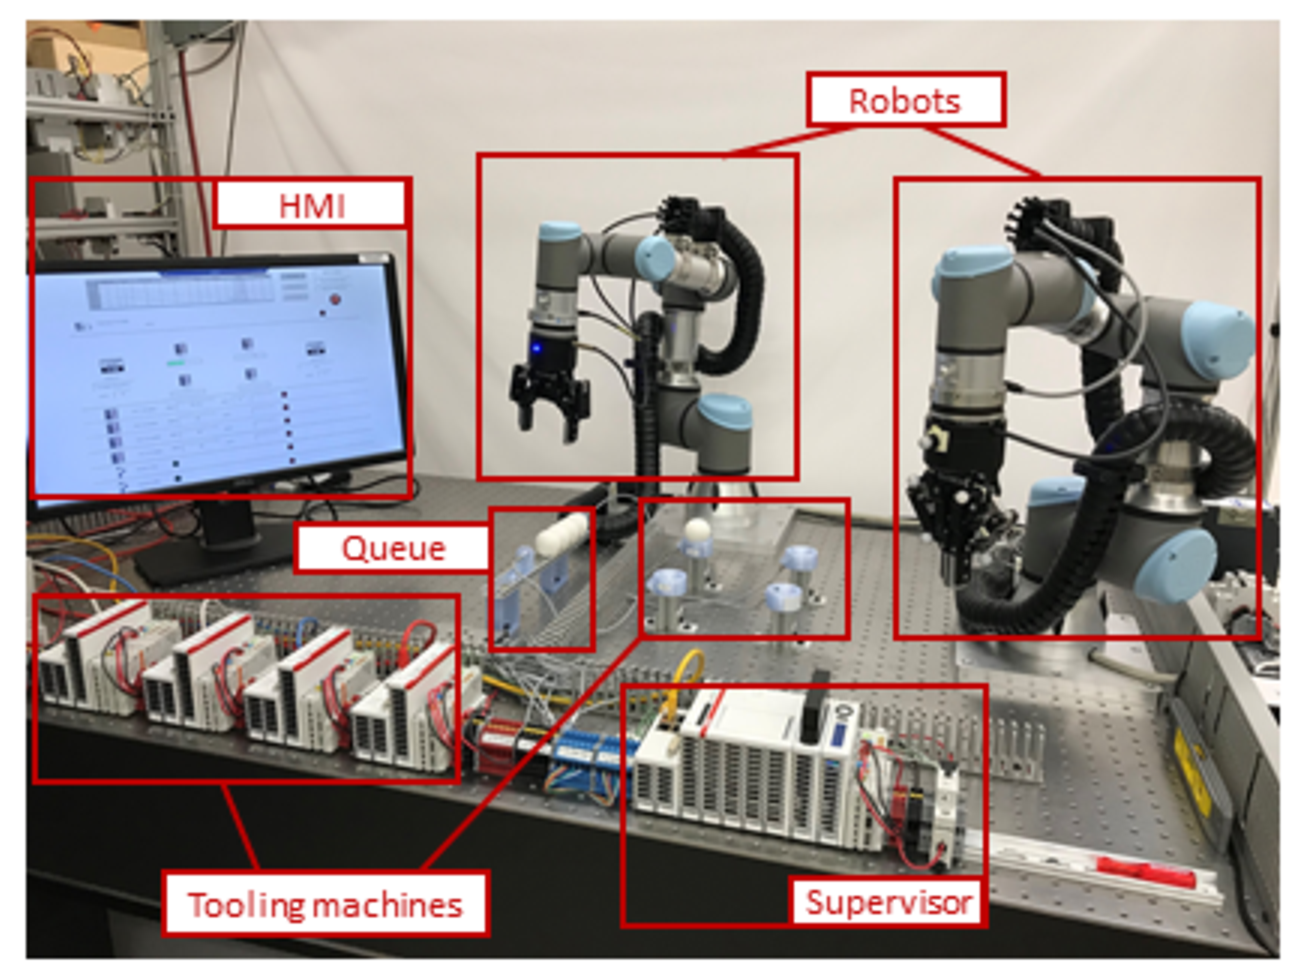
\includegraphics[width=\textwidth]{./chapter-gdb-appl/figures/cellShot}
	\caption{Collaborative work cell testbed}
	\label{gdbappl:fig::workcell}
\end{figure}

To facilitate wireless network research and showcase the power of wireless technologies in industrial practices, a testbed shown in Fig.~\ref{gdbappl:fig::workcell} has been developed at the National Institute of Standards and Technology (NIST) as described in~\cite{Liu2019vancouver}. The testbed is composed of two collaboration-grade robots, a supervisory programmable logic controller (PLC) used for the control of the workcell, four smaller PLCs serving as computer numerical control (CNC) machine emulators, and a human-machine interface (HMI).  Each robot is equipped with a six-degrees-of-freedom (DOF) force-torque (FT) sensor and a two-finger gripper. A Modbus/TCP server is included within the supervisor PLC and is used for communication between the supervisor and the robots.  The PLCs themselves communicate to each other using the Beckhoff Automation Device Specification (ADS) protocol. All elements within the workcell are synchronized to a stable and accurate grand-master clock. Therefore, as described in~\cite{Liu2019vancouver}, the operational, network, and measurement elements are all synchronized to the grand-master clock through a precision time protocol (PTP)-capable switch. 

Work-orders for the workcell are submitted through the supervisor. Each work-order consists of a work-plan for a part, and the work-plan determines how each part moves through the workcell until it is completed. The inspection of each part is conducted at each machining station, and after the final inspection, the part is placed back into the input queue.  Under normal operating conditions, the work continues until all work-orders have been processed.  This continuous form of operation provides ample opportunity to collect statistically significant metrics of both the network and the operation of the workcell.

\subsection{Database Schema}\label{gdbappl:sec::dbschema}

\begin{figure}[!ht]
	\centering
%	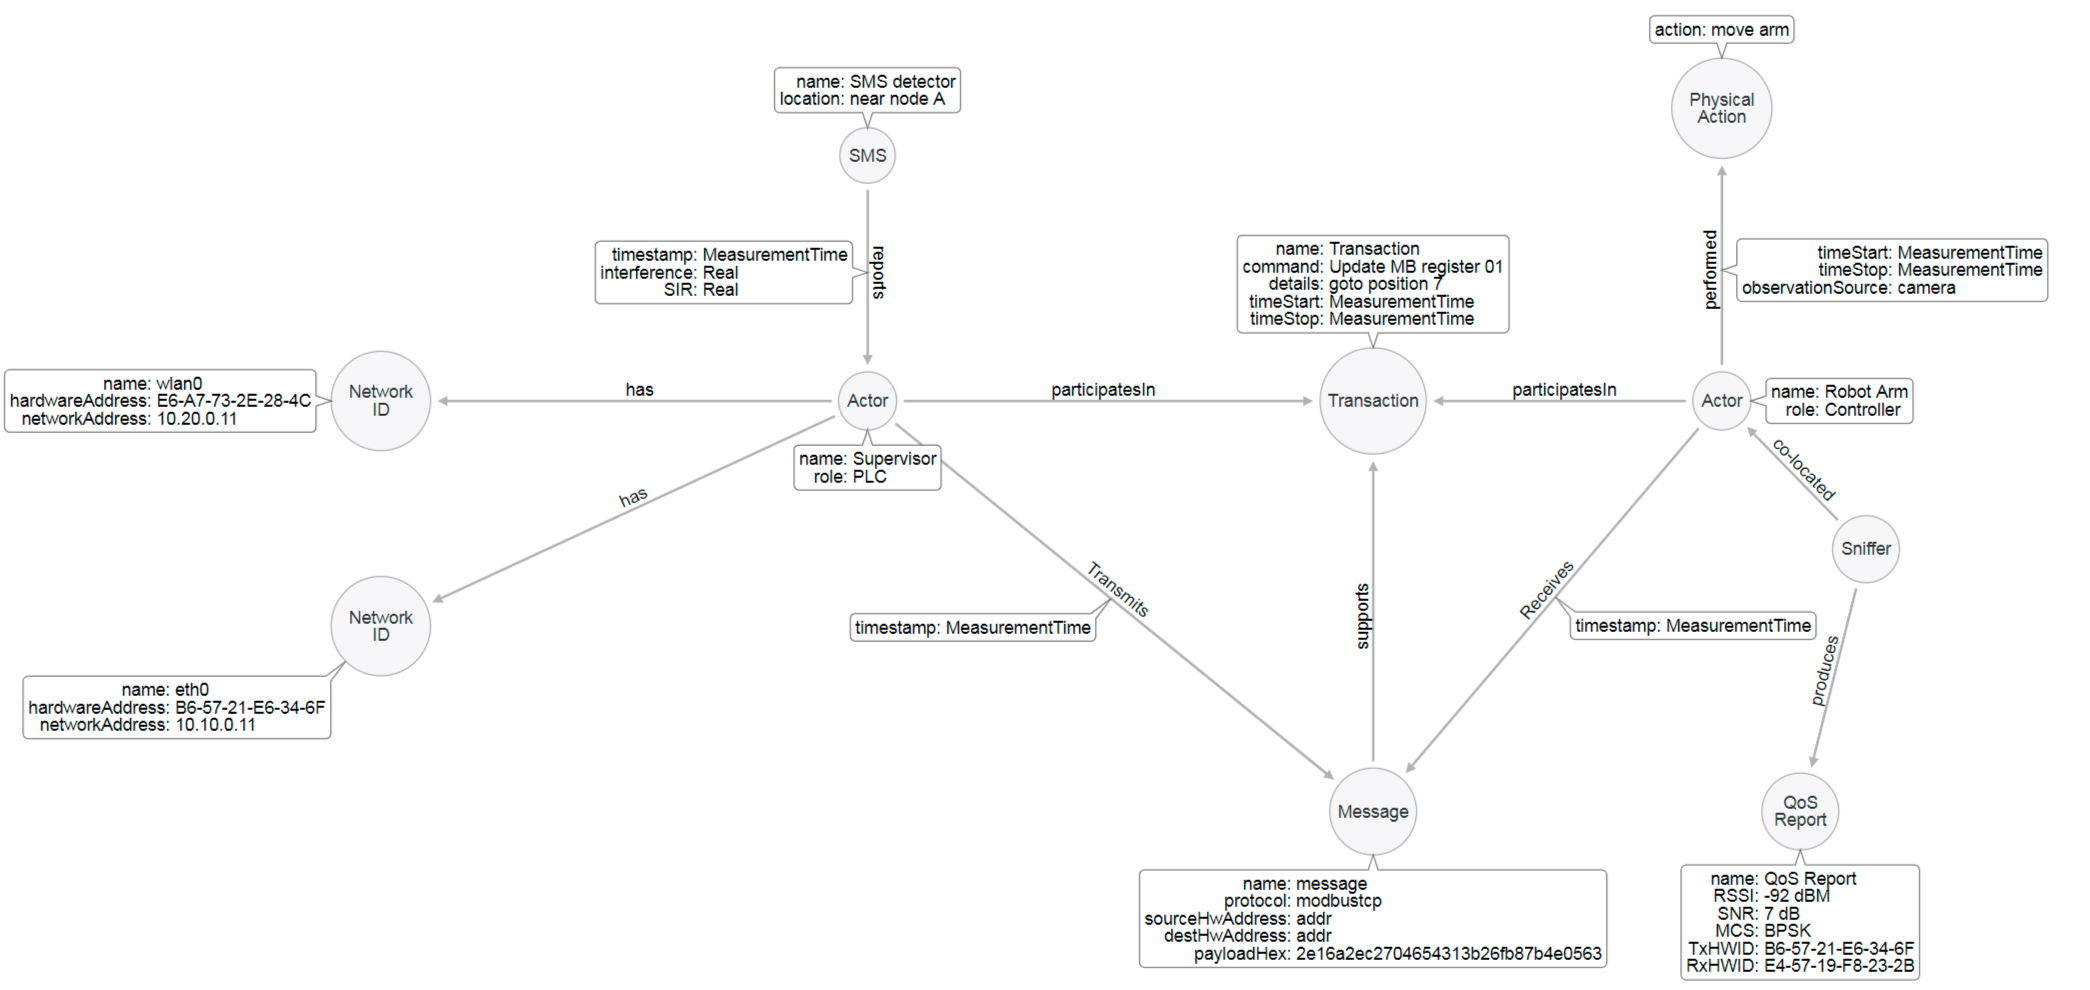
\includegraphics[width=\textwidth,trim=50 50 50 50, clip]{figures/database/arrows-schema.PNG}
	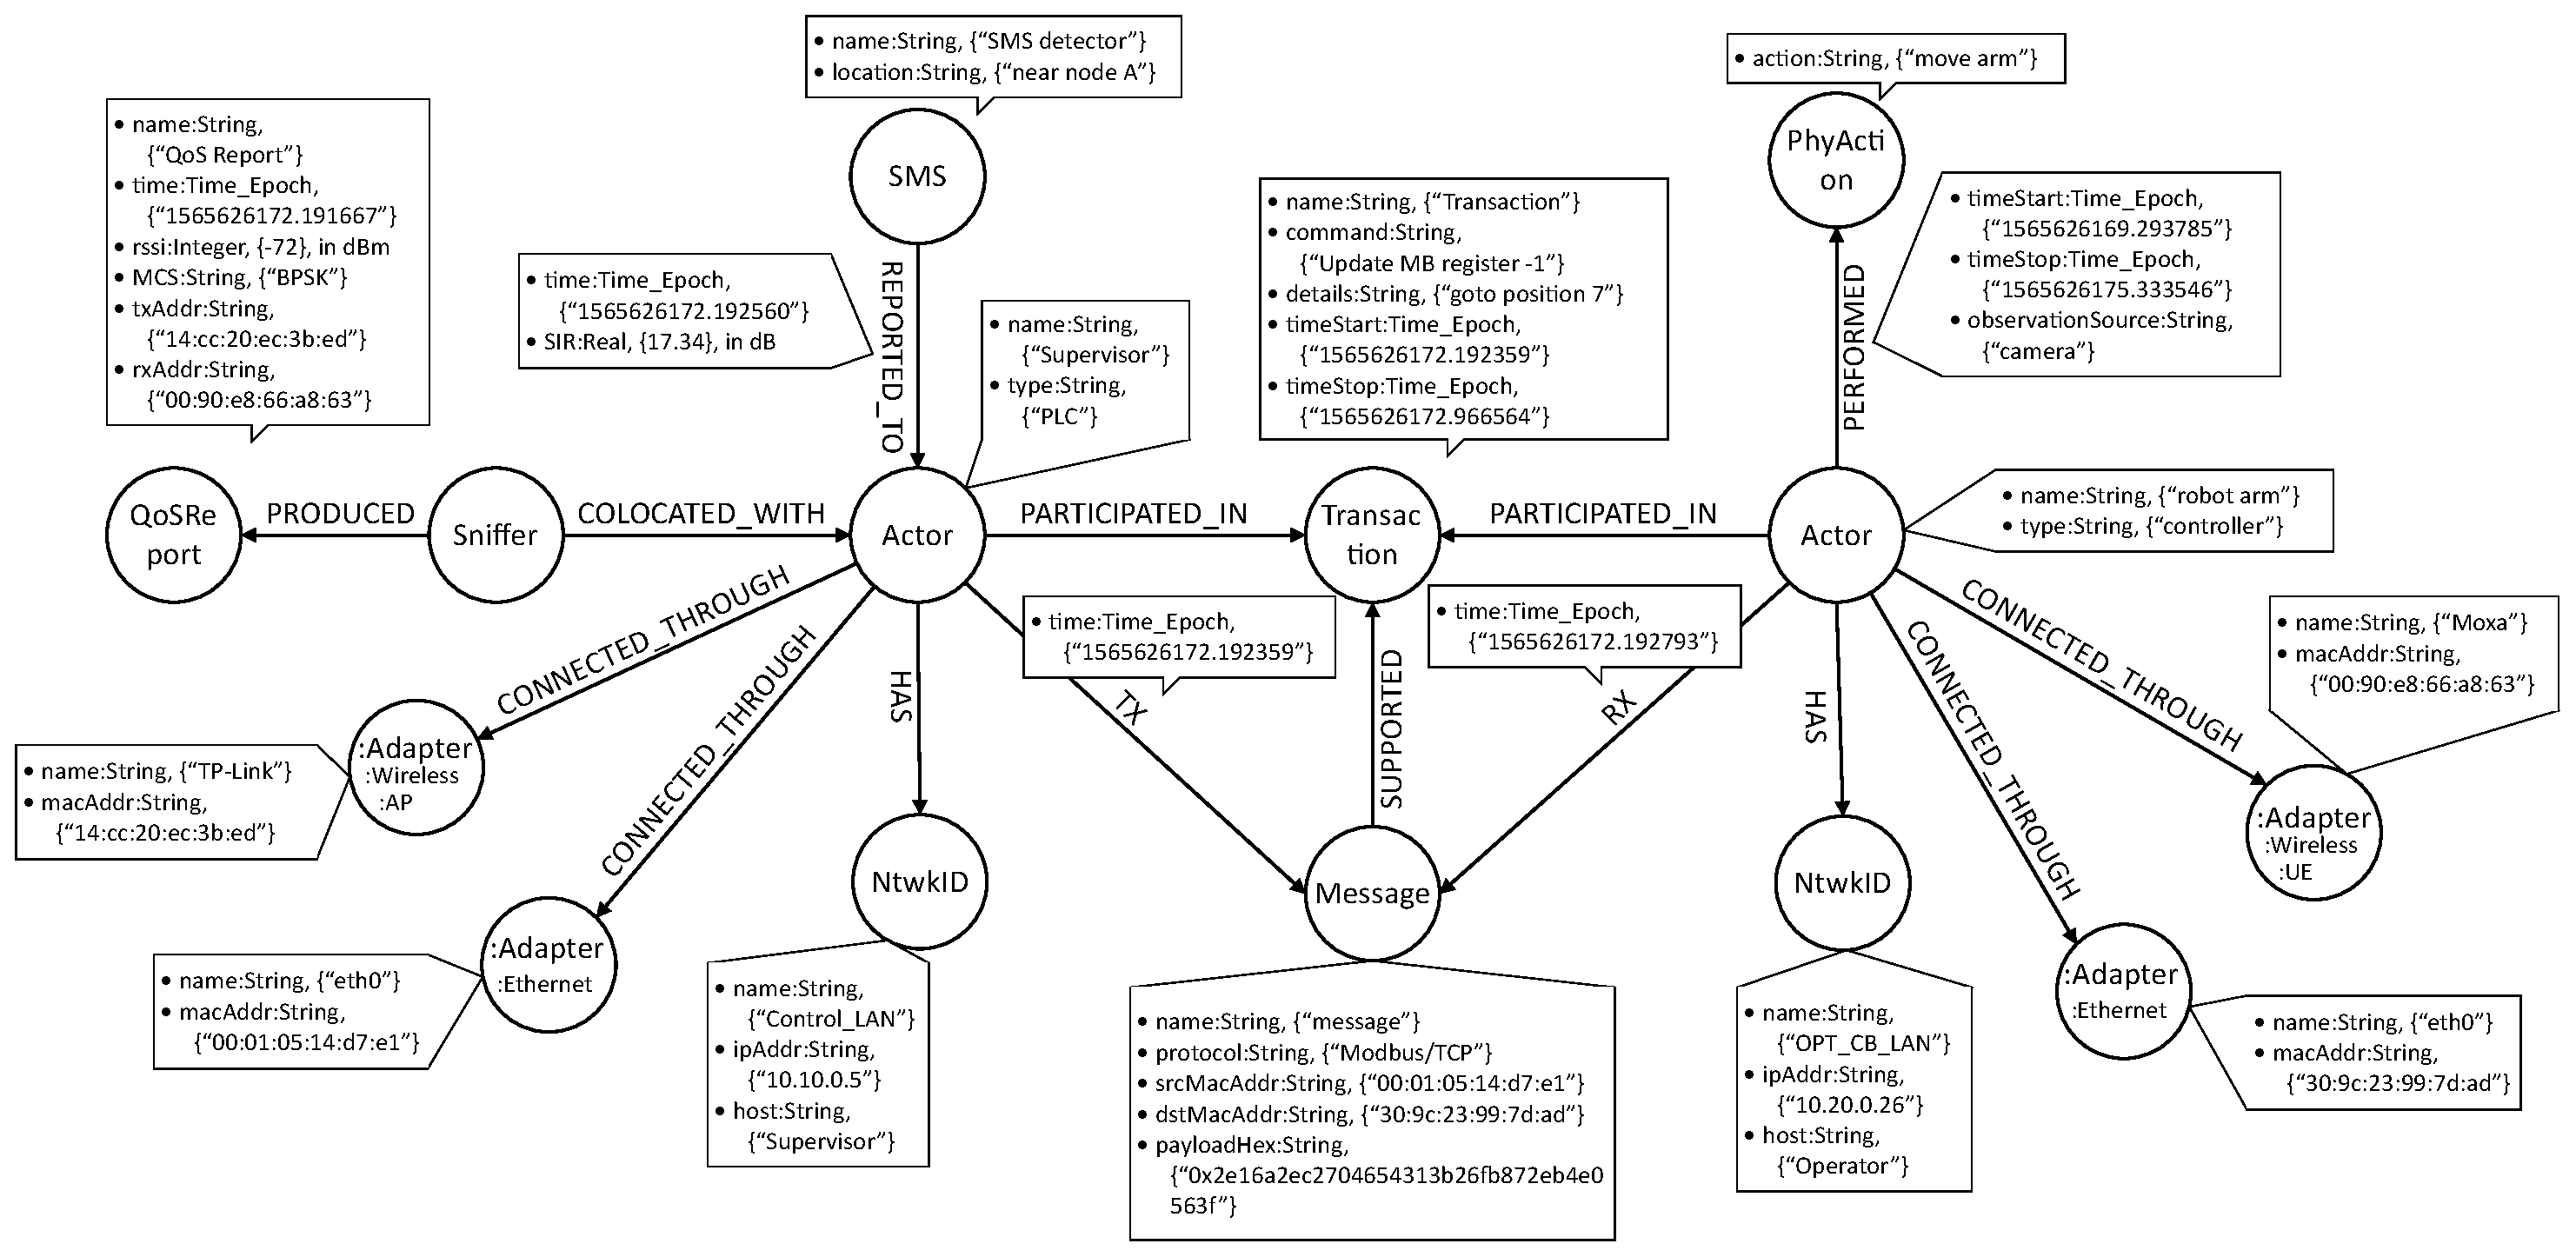
\includegraphics[width=\textwidth]{./chapter-gdb-appl/figures/database/graph_schema_0816.eps}
	\caption{The intended schema (i.e., pseudo-schema) of the graph database used for each operational run of the NIST wireless factory testbed.  The graph is organized into nodes and edges, where the edges signify relationships among network elements and physical operational elements.}
	\label{gdbappl:fig::database:schema}
\end{figure}

GDBs are NoSQL databases such that the database does not contain any predefined structure or rules to enforce such structure.  This is a major difference between relational databases and GDBs.  Nevertheless, it was necessary to sketch a pseudo-schema to capture the intended nodes and relationships that would be stored within the database (the terms pseudo-schema and schema will be used interchangeably). Before describing the schema itself, it is necessary to first explain the requirements of the schema.  Therefore, the requirements for the schema are as follows:

\begin{description}%[style=sameline]
% [Time] 
\item[Time] Any manufacturing automation system is indeed a time-varying control system with network and operational events.  The database schema must necessarily support time-based queries and, specifically, time-windowed 
queries.
% [Operational Events]
\item[Operational Events] The schema must represent operational events such as the movement of a robot arm or the movement of a part.
% [Network Events]
\item[Network Events] The schema must represent network events such as the transmission of packets.
% [Transactions/Grouping]
\item[Message Grouping]  The schema must support grouping of logically related events such that those events can be correlated to a specific occurrence within the testbed.
% [Wired/Wireless Support]
\item[Wireless Support] The schema must support the capture of both wired and wireless network traffic without special provisions within queries for either.
% [QoS]
\item[QoS Support] The schema must allow for the capture of quality of service (QoS) data when available.
% [Spectrum Monitoring]
\item[Spectrum Monitoring] The schema must support the capture and association of network events with observations from a spectrum monitoring system (SMS) if that information is available.
\end{description}

\subsubsection{Node Design}

Given the fore-mentioned requirements, a sample pseudo-schema is shown in Fig.~\ref{gdbappl:fig::database:schema}, which represents the intended structure of the information within the GDB. It is important to remember that since GDB schemas are not really schemas, such as those found in relational databases, but representations of intent, the schema represented here should be considered a notional example of the final product.  Within the graphs, nodes represent logical elements, and edges represent the relationships between those elements.  Both nodes and edges may contain properties providing more description and labels that define categories or classes of the said nodes or edges.  The schema is designed such that the data within the graph is intuitive to understand and allows for time-based queries to occur.  The facilitation of time-based queries was an essential requirement of the database design.  The schema is represented using the following node labels:

\begin{description}%[style=sameline]
    \item[Actor]  A physical component within the factory workcell such as a robot, PLC, or other networked item.
    \item[NtwkID] A network address item for an actor such as an Internet Protocol (IP) address.
    \item[Transaction] A complete information exchange between two or more actors (multiple actors may participate in a transaction).
    \item[Message] A network transmission event that occurs between two actors (messages are essentially packet transmissions captured at the transport layer; multiple messages support a transaction).
    \item[Physical Action]  A physical occurrence within a factory workcell associated with actors through multiple time based relationships.
    \item[SMS] An SMS observes and records significant spectral events within the workcell and may report those events to actors within the workcell.  
    \item[Sniffer] A measurement device that records all transmissions conducted over the wireless medium and includes wireless header information for each wireless transmission detected.
    \item[Adapter] A device that serves to connect an actor to a network (adapters are divided into sub-categories depending on the type of interface to a network).
    \item[Adapter:Ethernet] A subcategory of adapter representing an Ethernet interface. 
    \item[Adapter:Wireless] A subcategory of adapter representing a wireless interface. 
    \item[Adapter:Wireless:AP]  A subcategory of adapter representing a wireless access point interface.
    \item[Adapter:Wireless:UE] A subcategory of adapter representing a wireless user equipment interface.
    \item[QoS Report] A quality of service report of a message (not all messages will have a QoS report).
\end{description}

It is important to note that most network infrastructure components are not captured within the graph, but, instead, only basic interfaces between actors and the network are captured.  The intention when designing the graph was to make the graph network and protocol agnostic, such that the network is viewed as a black-box. Accordingly, the captured events of the physical system and the network are considered useful for the analysis of performance. 

\subsubsection{Relationships (Graph Edges)}
Relationships are edges within the graph that capture the informational interactions between nodes.  Relationships, like nodes, can contain labels and properties.  As shown in Fig.~\ref{gdbappl:fig::database:schema}, nodes are connected through defined relationships.  A subset of the relationships are defined as follows:
\begin{description}
    \item[PARTICIPATED\_IN] Actors will participate in transactions.  A transaction exists for each logical set of messages between actors such as the setting of a Modbus register or the sending of a command to a robot.  Therefore, actors will participate in many transactions, and multiple actors may participate in a single transaction.
    \item[SUPPORTED] Messages (i.e., packets between actors) are associated with transactions through the SUPPORTED relationship. Depending on the protocol and the quality of the channel, a single transaction could have one or many messages connected through this relationship.
    \item[TX/RX] An actor may either transmit (TX) or receive (RX) a message. Both the TX and RX relationships contain a timestamp in the format of an epoch time which is a floating point number in seconds since January 1, 1970, with a resolution of microseconds.
    \item[PERFORMED] When an actor performs a physical action, a relationship is created between the actor and the physical action node. This relationship contains start and stop time properties as well as the source of the observation such as a networked camera.
    \item[REPORTED\_TO] An SMS may be a passive or active listener within a workcell.  When an SMS operates as an active listener, spectral reports from the SMS may be sent to an actor such that the actor can respond intelligently to the spectral event.  Reports from an SMS to an actor are captured within this relationship.
\end{description}
Other relationships shown in the schema of Fig.~\ref{gdbappl:fig::database:schema} but not explained above are considered self-explanatory.

\subsubsection{Closer Examination}
Examining the sample schema more closely, two actor nodes are represented.  In this case, Actor A is the supervisory controller, and Actor B is a robot arm.  Both nodes participate in a transaction, which, in this example, is a Modbus/TCP exchange. The transaction itself is associated with one or more messages (i.e., packets). Each message associated with a transaction manifests itself as a node in the graph. Multiple message nodes will exist for each transaction. 
%It is important to note that a timestamp is not recorded for each message.  The reason is that the timestamp for a message is captured in the edge relationships between the sender and the message and the receiver and the message.  Thus, a timestamp for transmission and reception are recorded within the graph through the TX/RX relationships.  
Additionally, QoS reports may be associated with each actor node through a collocated sniffer node.  By keeping QoS reports separate, the flexibility of supporting different wired and wireless protocols within the same graph is maintained. Recall, that a graph database has no enforceable structure and thus affords this type of flexibility. Each actor node may have network identities associated with it through the use of network identifier nodes.  Each network identifier node may contain address information such as a hardware address or a network address; however, this is dependent on the protocols and addressing schemes being used, and a node could have many different identification nodes. 
\subsubsection{Physical Actions}
Finally, each actor in the graph may associate with physical actions.  These actions exist in the database as automatons such that every time a new action occurs, a new edge would be added between the actor and the physical action.  Timestamps within the graph represent ``measurement time'' denoting that all  timestamps are accurately synchronized to the grand-master clock.  The method of synchronization is outside the scope of this paper and is explained fully in~\cite{Liu2019vancouver}.  This paper describes the database structure and the process for preparing and inserting the data into the database, which is described in the following subsection.

\subsection{Information Workflow}

\begin{figure*}[!ht]
    \centering
    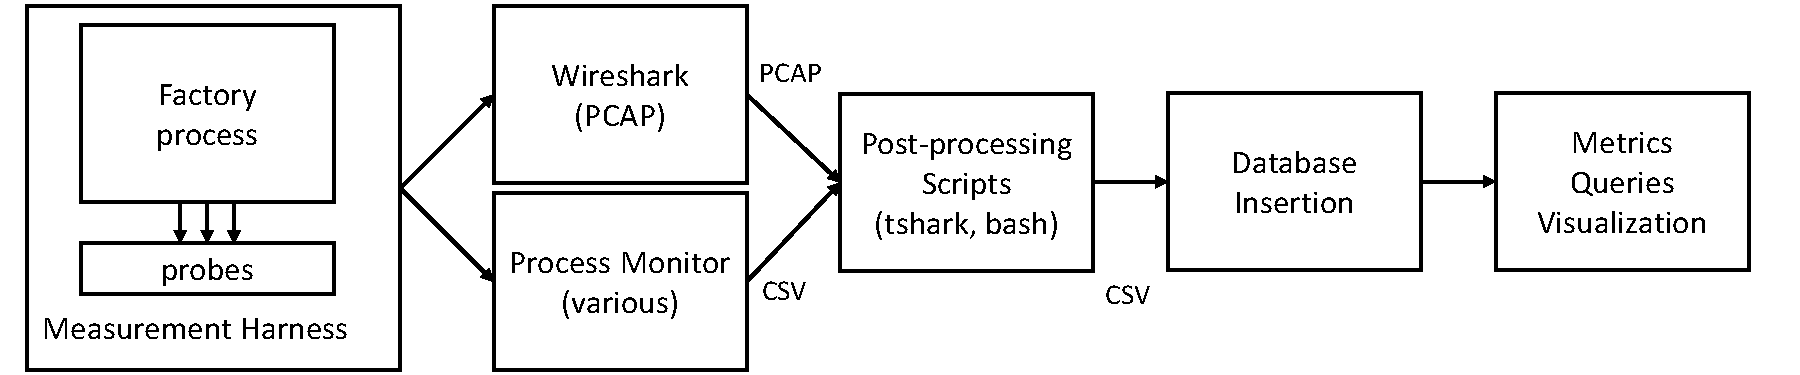
\includegraphics[width=0.95\textwidth]{./chapter-gdb-appl/figures/database/work-flow.pdf}
    \caption{Data processing flow from factory workcell to database}
    \label{gdbappl:fig::work-flow}
\end{figure*}

The workflow for collecting, processing, and inserting measurement data into the graph database is multi-pronged, as shown in Fig.~\ref{gdbappl:fig::work-flow}.  The workcell, which in this case study is a two-robot workcell with four CNC machines, is instrumented with network probes that capture transmitted and received packets as well as probes to capture operational movements such as arm robot position and the state of the supervisor PLC.  Network data is stored in packet capture (PCAP) files, while operational data is stored in comma separated value (CSV) files. Bash scripts were developed to extract relevant information and prepare the data for insertion into the database. The scripts also contain rules for grouping packets together as transactions based on the application protocol and time. The scripts produce CSV files that are ready for insertion into the Neo4j database.  Once the data resides within the database, queries are applied to extract information for the evaluation of workcell performance and visualization of network and operational events within the workcell. By tracking paths through the relationships within the graph, discerning how a network event such as interference is related to physical events such as position uncertainty or part throughput is possible. Various impairments may be introduced as a part of workcell operation.  Examples of such impairments include competing wireless traffic, radio interference, and reflections and diffraction due to the multi-path environment~\cite{Candell2017.NIST1951}. It is also feasible to implement such impairments and measure the resulting physical performance manifestation~\cite{Liu2019vancouver}. This is accomplished through the use of a radio channel emulator as demonstrated in~\cite{CandellISIE2019.Conf}.

\subsection{Sample of a Resulting Graph}
In the following, this investigation shows the results from a trial run of the NIST industrial wireless testbed. In this trial run, a single physical wireless link is used between a wireless adapter connected directly to the supervisor and a wireless access point connected to all the other actors in the testbed. The wireless nodes represent IEEE 802.11b/g/n devices and are connected through a variable radio frequency (RF) attenuator that allows us to vary the channel quality. During the trial run, the production of 10 parts was emulated, which resulted in 10 minutes of network activity.       

After populating the database with data captured from the trial run, the resulting realized schema is shown in Fig.~\ref{gdbappl:fig::real-schema}. The schema visualization is produced by invoking the command

\begin{lstlisting}
call db.schema.visualization()
\end{lstlisting} 
in Neo4j. It is important to note that a realized schema shows only one representation of each node and relationship whereas the intended pseudo-schema shown in Fig.~\ref{gdbappl:fig::database:schema} was developed to exemplify the relationships between types of nodes, labels, and relationships. Where label inheritance is employed, such as the case for different adapter types, relationships are reproduced; however, this is a result of the visualization tool rather than the schema itself.  Fig.~\ref{gdbappl:fig::real-schema} serves, therefore, to validate that the intended schema was indeed realized by the insertion of event data from the testbed. In the realized schema, inherited labels are shown as separate nodes.

\begin{figure}[!ht]
    \centering
    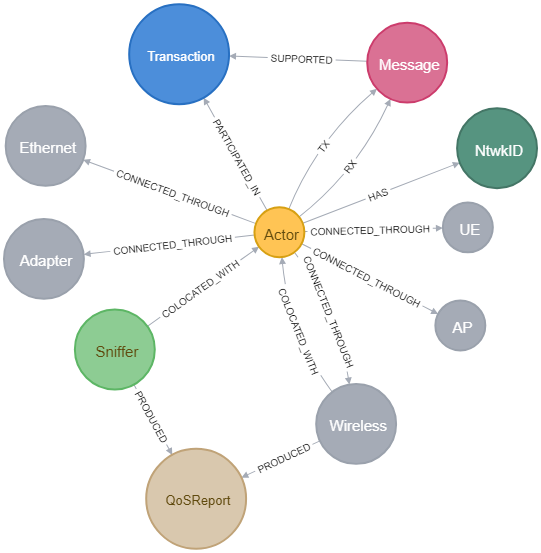
\includegraphics[width=0.65\columnwidth]{./chapter-gdb-appl/figures/database/graph_schema.png}
    \caption{Realized schema of the graph database fully populated after capturing network and operational data from the NIST industrial wireless testbed. }
    \label{gdbappl:fig::real-schema}
\end{figure}

As described in Section~\ref{gdbappl:sec::dbschema}, the database includes every network transaction that occurs during the operation of the testbed.  This includes any logical transaction nodes inserted into the database and any associated packets that happened to traverse the network.  Therefore, for a short duration of time depending on packet transmission rates, the amount of data stored in the database can grow quickly. This presents a visualization challenge that graphs are designed to handle. A sample graph is shown in Fig.~\ref{gdbappl:fig::Sample-graph_1}, which represents only 1 second of wired and wireless network data captured from the NIST two-robot pick-and-place wireless testbed described in~\cite{Liu2019vancouver}. 

\begin{figure}[!ht]
    \centering
   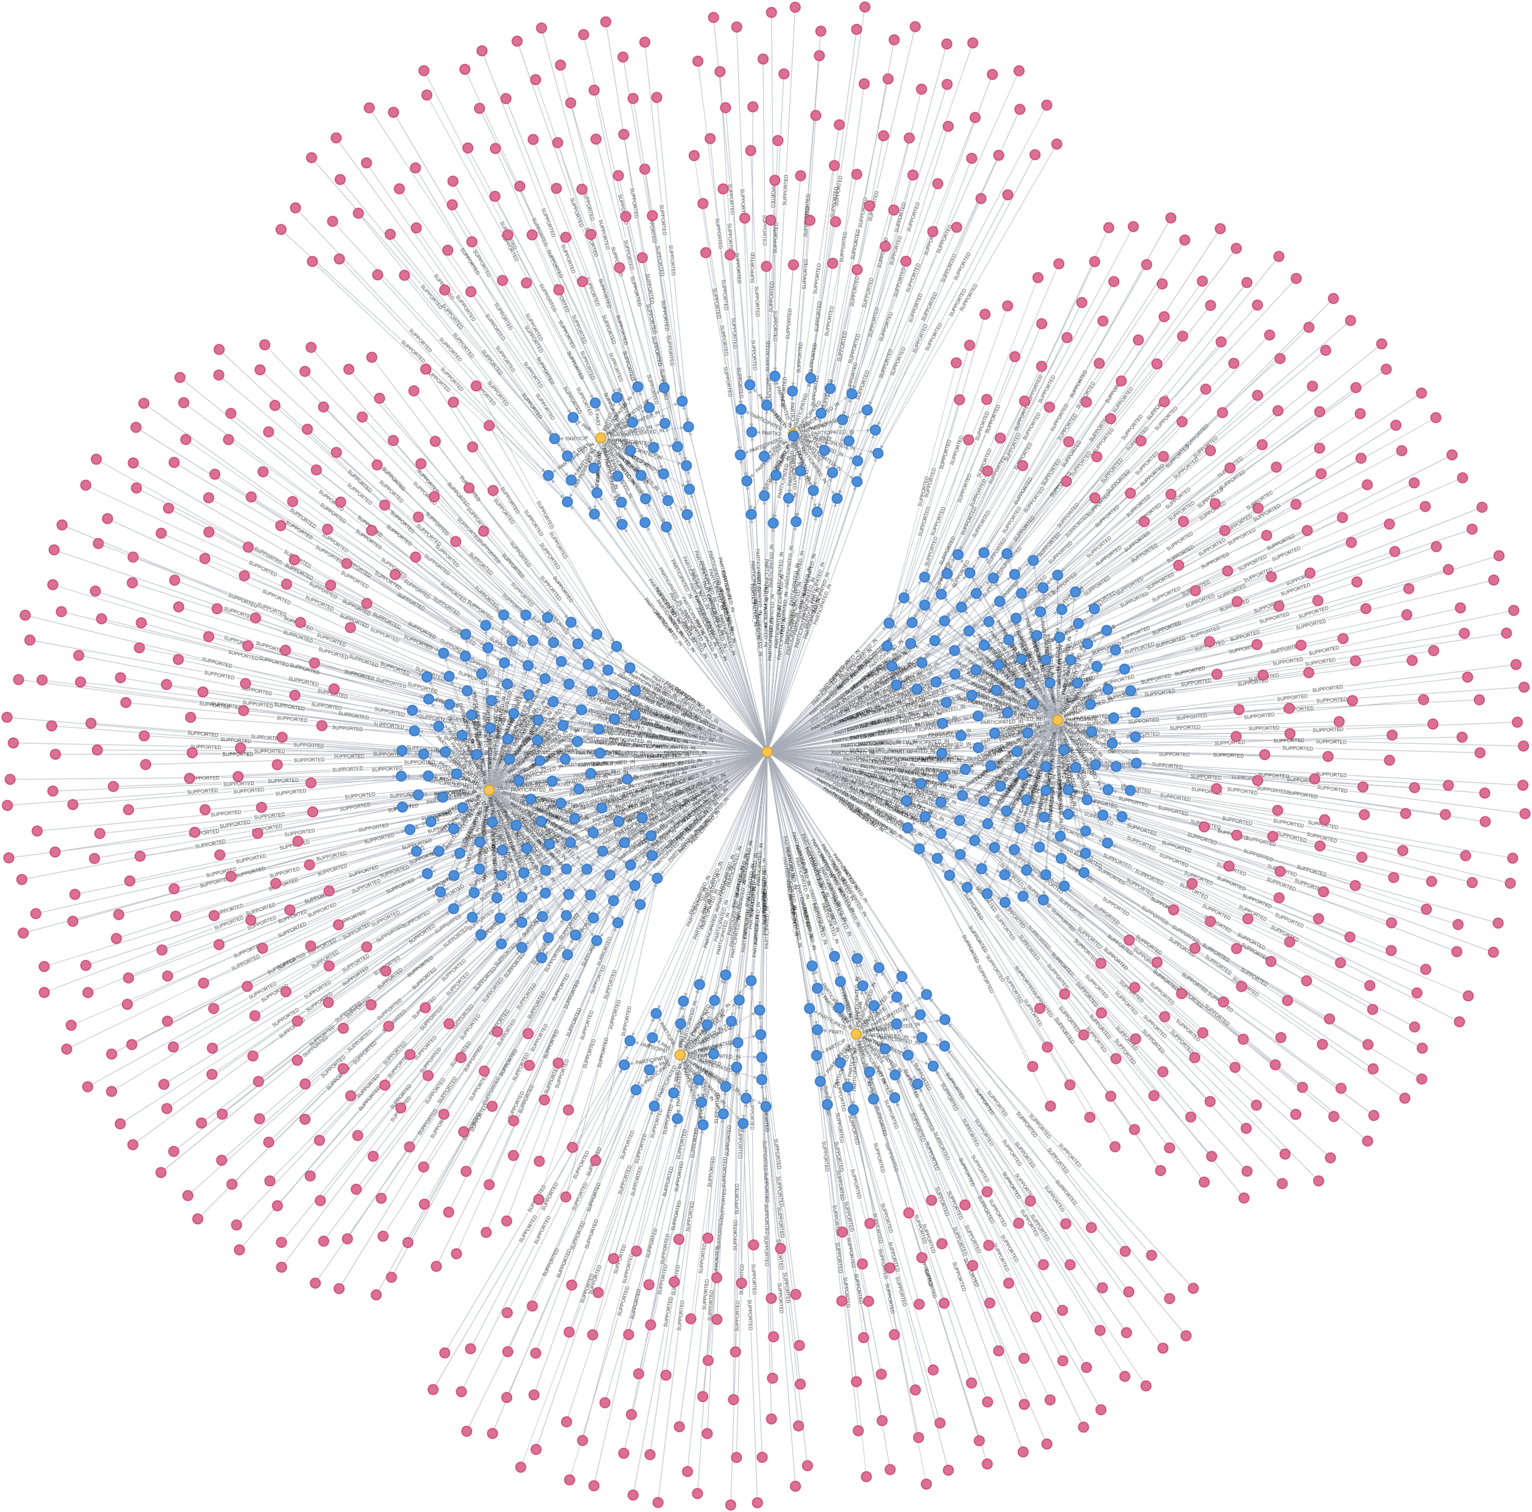
\includegraphics[width=0.85\textwidth]{./chapter-gdb-appl/figures/database/graph_M_T_2.png}
   \vspace{0.1in}
    \caption{ Visualization of a node graph resulting from a testbed experiment. }
    \label{gdbappl:fig::Sample-graph_1}
    \vspace{0.1in}
\end{figure}

This visualization is produced by calling the following query in the Neo4j. 
\begin{lstlisting}
MATCH p=(a:Actor {name:'Supervisor'})--(t:Transaction)--(b:Actor) ,p2=(m:Message)-->(t) WHERE t.timeStart>T AND t.timeStop<T+1
RETURN p,p2
\end{lstlisting}

The colors of the resulting nodes follow the realized schema in Fig.~\ref{gdbappl:fig::real-schema} while only the actors, transactions, and messages are visualized in Fig.~\ref{gdbappl:fig::Sample-graph_1}. The relationships between the messages and transactions are shown where a single transaction is connected to at least two messages to represent the communications between any two actors. The variable T in the query represents an arbitrary time variable in seconds within the trial run to capture the data within 1 second only.

The visualization then show a more detailed visualization for all the nodes and relationships corresponding to a single transaction. It is produced by calling the following query where Ts is an arbitrary time variable to specify the timeStart value for the single transaction. 

\begin{lstlisting}
MATCH p=(a:Actor {name:'Supervisor'})-->(t:Transaction {timeStart:Ts})<--(b:Actor {name:"CNC-1"})
WITH p, a, b, t
MATCH p1=(a)-->(m:Message)<--(b), p2=(m)-->(t), p3=(a)-[:HAS]-(),p4=(a)<-[:COLOCATED_WITH]-()-[:PRODUCED]->(q:QoSReport), p5=(a)-[:CONNECTED_THROUGH]-(),p6=(b)-[:HAS]-(), p7=(b)-[:CONNECTED_THROUGH]-()
WHERE q.time>t.timeStart AND q.time<t.timeStop
RETURN p,p1,p2,p3,p4,p5,p6,p7
\end{lstlisting}

In Fig.~\ref{gdbappl:fig::Sample-graph_2}, the actor nodes are labeled by their names \textit{CNC-1} and \textit{Supervisor}, the transaction is labeled by its type \textit{ADS}, the messages are labeled by their transmission role \textit{Request} and \textit{Response}, the NtwkIDs are labeled by their IP addresses, the Ethernet adapters are labeled by their names \textit{eth0}, the wireless adapters are labeled by their names \textit{Moxa} and \textit{TP-Link}, the sniffer is labeled by its name \textit{WLS1}, and the QoS reports are labeled by the received signal strength indicator (RSSI) value in dBm. This visualization includes only the QoS reports generated within the duration of the corresponding transaction.   

\begin{figure}[!ht]
    \centering
    \includegraphics[width=0.95\textwidth]{./chapter-gdb-appl/figures/database/graph_Single_trans.png}
    \caption{A detailed visualization resulting from a testbed experiment for all the nodes and relationships corresponding to a single transaction. }
    \label{gdbappl:fig::Sample-graph_2}
\end{figure}

\subsection{Calculation of Metrics}

\begin{figure}[!ht]
	\centering
%	\includegraphics[width=\textwidth,trim=50 50 50 50, clip]{figures/database/arrows-schema.PNG}
	\includegraphics[width=0.5\textwidth]{./chapter-gdb-appl/figures/database/scatter_1.eps}
	\caption{Correlation between the message latency and the RSSI values by the sniffer.}
	\label{gdbappl:fig::database:scatter}
\end{figure}

An example of deploying the proposed GDB approach in industrial wireless analysis is now presented. During the trial run time, an RF attenuator value is varied for the single wireless link. The attenuation can take the values \{0, 10, 20, 30, 40, 50, 60\} dB. Message latency is evaluated as the difference between the receive and transmit times of a message including transmission, processing, and retransmission times. Each message has been coupled to a QoS report that is the one reported at the closest time instant before the message transmit time. One of the parameters in the QoS report is the RSSI value captured by the Sniffer colocated with the supervisor's wireless adapter. 

In Fig.~\ref{gdbappl:fig::database:scatter}, a scatter plot is presented showing the correlation between the message latency in seconds to the measured RSSI values by the sniffer in dBm.  The figure shows that the latency is higher at the lower RSSI values due to the increased number of retransmissions. Generally, an IEEE 802.11 transmission can occur using different IEEE 802.11 mode and modulation and coding scheme (MCS) based on the channel quality. At the RSSI of -90 dBm, the receiver should operate at the most robust communications mode and the lowest MCS index. However, retransmissions still occur due to having the received power near the sensitivity of the supervisor's wireless adapter. As shown in Fig.~\ref{gdbappl:fig::database:scatter}, retransmissions may occur at other RSSI values as well when the transmitter selects a higher mode of transmission and a higher MCS index. In this case, it is asserted that the receiver is operating close to the marginal sensitivity for a given mode (e.g., 802.11n) and MCS index.  It is observed that the transmitter switches to a lower MCS index for the retransmitted messages, which supports the supposition. Therefore, latency can in fact be high for better RSSI values.  This effect is illustrated in Fig.~\ref{gdbappl:fig::database:scatter} where certain messages can have latency values at -43 dBm, which are comparable to those in the case of  -90 dBm.  

%SAMPLE CALCULATION FOR REDUCED GRAPH SHOWN ABOVE OVER A SMALL PERIOD OF TIME
%* network delay
%* correlate power level to delay
%* show the cypher command for computing this stuff

%TALK ABOUT LATER: SAMPLE CALCULATION OF PERFORMANCE DEPENDENCY OF THROUGHPUT TO NETWORK PERFORMANCE ON A SLIDING WINDOW

\section{Case Study Elaborated: Robotic Machine-tending}
In this section, we present a two-robot machine tending work-cell case study as an elaboration of the previous study.  The two case studies are almost identical,; however, they were conducted sequentially as separate investigations.  In this study, the design of the work-cell, measurement system, and equipment used are presented along with the additional information within the results discussion. 

\subsection{Work-cell Physical Implementation and Measurements}

A work-cell was constructed to perform a dual robot pick-and-place task that is controlled by a supervisor programmable logic controller (PLC). The robots have six degrees-of-freedom which utilize Modbus/TCP communication messages to receive and then execute assigned tasks from the supervisor PLC. There are also four emulated computer numerical control (CNC) machines that detect the physical state of the testbed with proximity sensors. The workflow of the pick and place task involves the Operator moving parts from the queue ramp to each of the emulated CNC machines and back to the queue ramp. Between the Operator movements, the Inspector preforms a force seeking action to detect if the part is in the correct location before the Operator proceeds. More details on the exact workflow and a photograph of the testbed can be found in~\cite{Liu2019vancouver}. 

\begin{figure*}
	\centering
	\includegraphics[width=\textwidth]{chapter-gdb-appl/figures/Fig1TiiSpecialDiagram-testbed2}
	\caption{Network diagram of the industrial wireless testbed at NIST. Solid lines represent Ethernet based communications and dashed lines represent wireless based communications.}
	\label{gdbappl:fig::database:netdiagram}
\end{figure*}

All communicating devices on the testbed have been originally designed to use Ethernet TCP/IP for communication. To enable wireless within the testbed, Ethernet-WiFi bridges are utilized for wireless communications through a common access point (AP). To establish these Ethernet-WiFi bridges, Next-line-of-Computing (NUC) computers, are used.  NUCs are a line of small-form-factor barebone computer kits designed by Intel.   Each NUC in our experiments is configured in one of various forms as a bridge, a wireless sniffer, a traffic generator, or a traffic sink. These configurations in the network are shown in Fig.~\ref{gdbappl:fig::database:netdiagram}.

There are three different types of measurements (network, robot, and PLC state data) collected on the testbed. Network traffic data is captured using seven test access point (TAP) devices and a wireless sniffer, shown in Fig.~\ref{gdbappl:fig::database:netdiagram} with green labels. A machine running Ubuntu 18.04, not shown, is used to capture all wired network traffic on the testbed. The position and robot state data is captured from the robot controllers using the real time data exchange (RTDE) protocol~\cite{RTDE}. RTDE data is also captured on the Linux machine using the connected switches to each of the robot controllers. Lastly, the PLC state data is captured locally on the supervisor PLC during the experiment. These three types of measurements (network, robot, and PLC state data) have a shared precise time from the synchronization to the grand master time server. The design adopts the IEEE 1588 precision time protocol (PTP) to allow synchronized distributed clocks to stamp the accurate time to the measured network and operational events in the testbed~\cite{IEEE-Std-1588-2008-redline}.

\subsection{Equipment Used}

The following equipment are illustrated in Fig.~\ref{gdbappl:fig::database:netdiagram} for reference.
To enable wireless on the testbed, Intel NUCs running Ubuntu 14.04 are used which communicate through a common AP. The AP is a Netgear AC1900 wireless router. For the wired communications, we use two Cisco IE 4000 industrial grade Ethernet switches that are PTP compatible for time synchronization. The collaborative robots that preform the pick and place task are Universal Robots “UR3” CB series. The robots are also equipped with OnRobot HEX-H Force/Torque sensors which are used by the Inspector to inspect parts. The Supervisor PLC is a Beckhoff CX2020 with a EL6688 PTP module for time synchronization. The CNC simulators are Beckhoff CX9020 PLCs. The seven TAP devices on the testbed are SharkTap Gigabit Network Sniffers. To synchronize the timing of the devices while taking measurements, a Meinberg Lantime M900 grand master time server is used. Lastly, the Operator and Inspector each use a D-link DGS-108 8-port unmanaged Ethernet switch for wired communications between the robot controller and force-torque sensor and for the Linux machine to collect RTDE data through a wired connection.

\subsection{Building the Graph} \label{gdbappl:sec:graph}

A GDB was built to manage data collected from testbed measurements of both network traffic and physical operations.
% Save for later -YL
%Compared with relational databases, GDBs as NoSQL databases don't specify any predefined data structure or rules to enforce such a structure. Instead, GDBs treat individual data records as distributed node entities in a random graph and identify relationships as part of database components that link different nodes together. This feature enables GDBs to catch varying states and dynamics in a complex system and gradually improve data management along with better understanding of the system.
In this section, we briefly introduce graph components developed for our testbed and the data processing flow that transforms measurement results to graph entities. 

\subsubsection{Reference Data Model}
%Save for later -YL
%In a GDB, the data model, which can be roughly analog to the ``schema'' of relational databases, illustrates how data records are organized and stored in a graph. However, unlike a fixed schema, the data model of GDBs has more flexibility of depicting diverse data types, content, and connections between different entities whose structure and property profile can update and evolve with more data and/or better observation. A data model contains different node types with specific properties in the graph and various relationships between them. 
In the previous case study, we identified the requirements of a GDB data model and built a graph containing nodes and relationships that mainly exhibit information around networked industrial devices in a factory work-cell. In this continuation of the work, we further populate the earlier defined work-cell data graph by introducing additional node types characterizing physical actions that are newly captured. Accordingly, we update the relationships, such as associating individual quality of service (QoS) report data from the wireless sniffer with the packets captured at the collocated receiver. The updated data model provides a comprehensive view of production operations, information flows, and wireless channel variations in the testbed which facilitates further analysis work.  

\begin{figure*}
	\centering
	%	\includegraphics[width=\textwidth,trim=50 50 50 50, clip]{figures/database/arrows-schema.PNG}
	\includegraphics[width=\textwidth]{chapter-gdb-appl/figures/graph_schema_1209.eps}
	\caption{The data model of the graph database used for each operational run of the NIST wireless factory testbed.  The graph is organized into nodes and edges, where the edges signify relationships among network elements and physical operational elements.}
	\label{gdbappl:fig:database:schema}
\end{figure*}

As shown in Fig.~\ref{gdbappl:fig:database:schema}, an example is illustrated here that summarizes nodes, relationships, and their key properties used in the GDB. We will elaborate the definition and use of these entities in the remainder of this section.			


\paragraph{Node Design}

%To effectively depict testbed operations in the measurement, we define a series of node types in the graph. 
Nodes are GDB elements that are used to identify testbed components, device states, and messages that store snapshots of the testbed for further analysis. They can be found in two main classes depending on what type of objects the node represents.

The class of \textit{static} nodes covers testbed setup profiles which contain testbed components, network interfaces, and their settings. These entities are normally predetermined or collected in the initialization of each measurement. They usually remain constant in each round of measurements. This class includes Actor, Network ID (NtwkID), Spectrum Management System (SMS), Sniffer, and Adapter in the GDB. The Adapter nodes can further have additional labels to identify their network interfaces and the roles they play, such as Ethernet/Wireless and AP/user equipment (UE).

The class of \textit{dynamic} nodes in the graph captures various system events such as machine status reports, network traffic, and information flows in the testbed. These nodes are dynamically added into the graph whose quantities and properties are determined by the measured data. Such node labels include Transaction, Message, QoSReport, and Physical Action (PhyAction). Considering the diversity of measured testbed operations, PhyAction nodes have sub-class labels including URSchedule (for the Supervisor), SensorState (for CNC), and RouteState (for robots).


\paragraph{Graph Relationships}

A relationship in the graph denotes an action taken to associate two nodes, either homogeneous or heterogeneous ones, which shows their connections in the topology, timeline, or affiliation. The relationships used in the GDB were introduced in~\cite{CandellISIT2020.Conf}. As shown in Fig.~\ref{gdbappl:fig:database:schema}, most of them are self-explanatory. 

\begin{figure*}
	\centering
	%	\includegraphics[width=\textwidth,trim=50 50 50 50, clip]{figures/database/arrows-schema.PNG}
	\includegraphics[width=\textwidth]{chapter-gdb-appl/figures/info_workflow_tii.eps}
	\caption{Data processing flow from factory work-cell to database}
	\label{gdbappl:fig:database:work-flow}
\end{figure*}

\paragraph{Closer Examination}
The graph data model is designed in a way where nodes and relationships are centered around Actors. Actors have dual roles in the work-cell operations. In the factory system, Actors participate in the production operations.
In the example of Fig.~\ref{gdbappl:fig:database:schema}, two Actor nodes are presented. In this case, Actor ``Supervisor'' is the supervisory controller, and Actor ``Operator'' is a robot arm. The Supervisor schedules the production, collects the other Actors' states, and hosts supportive services, such as SMS. The Operator follows the instructions of the Supervisor and moves parts between work stations. Meanwhile, Actors also act as communication nodes which exchange messages between each other through various network interfaces. In Fig.~\ref{gdbappl:fig:database:schema}, Actors participate in a transaction, which, in this example, is a Modbus/TCP exchange. The transaction itself is associated with one or more messages (i.e., packets). Each message associated with a transaction manifests itself as a node in the graph. Multiple message nodes will exist for each transaction. Additionally, QoS reports may be associated with each actor node through a collocated sniffer node.  %By keeping QoS reports separate, we have the flexibility of supporting different wired and wireless protocols within the same graph.

Dynamic event nodes in the measurement, i.e., physical actions, network messages, information transactions, and QoSReport records, have timestamps representing ``measurement time'' of the recorded events. Once a new event occurs, a proper relationship would be added between the actor and the physical/network event node. All timestamps are accurately synchronized to the grand-master clock.


\subsubsection{Information Workflow}

A multi-stage workflow is deployed to feed the graph with instances of nodes, relationships, and their properties that are extracted from measurement data, as shown in Fig.~\ref{gdbappl:fig:database:work-flow}. In the measurement data set, network data from distributed network probes in selected links is stored in packet capture (PCAP) files, while operational data that comes from different PLC and robot controllers is stored in the format of comma separated value (CSV) files. The whole process contains four steps including data preprocessing, feature extraction, database insertion, and post-import tuning. Such conversion from raw data to the ready-to-go graph has been done  by running automated scripts on a host machine which maintains data repositories of measurement results and deploys the Neo4j desktop application. The functions and operation features in individual steps are discussed next. 


\paragraph{Data Preprocessing}

Data preprocessing is the first step where measurement data is verified, cleaned, and formatted to facilitate the following processing steps. As fore-mentioned, measurement data contains results collected from heterogeneous modules/devices in the testbed which may adopt different data types, sampling rates, time and metric resolution, and file formats. For example, different machines may represent and store the record timestamps in various formats depending on local clock settings. Once we obtained the data, we unified the time representation in the entire data set using the time epoch that has microsecond resolution. In another example, we deployed packet filters to remove unrelated packet captures. In treating measurement data, e.g., experimenting with single or double wireless interference links, we managed to reduce the sniffer data in the order of gigabytes to only a few megabytes while keeping all signaling handshakes of interest in the studied links. 

\paragraph{Feature Extraction}

Feature extraction refers to the process of extracting relevant information from measurement data and prepare the data for insertion into the database. Nodes and relationships are defined by a set of features that share common views. We developed bash and Python scripts that pick the desired features to produce CSV files that are ready for insertion into the Neo4j database. In this step, a bash script was developed running the tshark tool to extract fields of protocol headers in packet captures and save the field information into CSV files. Each line in these CSV records will create one Message node instance as a sender or receiver copy of the packet through a link. A Python script was also used to detect state switches in the physical action data and label these moments which were triggered by testbed communications.


\paragraph{Graph Insertion}

We load the prepared data into the Neo4j GDB using bulk importing which can create one or multiple nodes and/or relationships in the graph by reading a CSV file once. 
Neo4j uses Cypher to construct GDB queries to import data.
As the output of feature extraction, each line of the CSV file can create one new node entity and/or generate the criteria of linking two qualified nodes for a new relationship. Properties of new entities can be assigned explicitly by the column values of records or inferred from predetermined rules such as some fixed combination of nodes and edges in the graph. Multiple types of nodes can be created from the same data file using one common node template in which each node type has its own subgroup of properties. For example, Modbus and ADS packets use the same Message node structure in our graph to manage the common transmission information such as IP addresses and TCP session identification. Meanwhile, each of these Messages maintains its own application layer header information in the node properties, e.g., Modbus register addresses and ADS function codes.   


\paragraph{Post-Import Tuning}

Post-import tuning refers to any additional modification in the graph after CSV data is imported. This step treats a few cases where raw data work with current graph insights to obtain new ones. First, in the additive insertion case, i.e., when new data is added into the graph, it links the newly added nodes to the existing ones following necessary relationships between them. Time series data often use this method to link consecutive event nodes in the recorded process.
Second, it is the case in which higher level features are needed in the graph which can be abstracted from the imported data. For example, Transaction nodes are built upon Message nodes who participate in the same application transactions; Message nodes themselves are also the summary of packet data, i.e., packet copies at link transceivers. Third, it can feed feature extraction with pieces of information in the current graph for purposes such as coupling data records. For example, coupling QoS reports and Messages in their observation windows used to be an extremely time-consuming process. On one hand, each Message raw data, i.e., the transmitter or receiver copy, contains only half of the transmission time window information. On the other hand, the Cypher query takes a long time to find all eligible relationships as Neo4j would generate a huge Cartesian product when treating the large sample set. We solved this issue by obtaining qualified Message nodes and feeding them into feature extraction where a more efficient Python script finds all Message-QoS Report pairs and later presents them in the graph as new COVERED relationships. 


The above four steps can perform multiple iterations to treat data and refine the graph according to the data complexity and requirements.  
%
\begin{figure*}
	\centering
	\includegraphics[width=0.8\textwidth,height=3.5in]{chapter-gdb-appl/figures/database/graph_schema_updated_2.png}
	\caption{Realized schema of the graph database fully populated after capturing network and operational data from the NIST industrial wireless testbed. \vspace{-0.2in}}
	\label{gdbappl:fig:real-schema}
\end{figure*}

\subsection{Results} \label{gdbappl:sec:results}

Once the data resides within the database, we apply queries to extract information for the evaluation of work-cell performance and visualization of network and operational events within the work-cell. By tracking paths through the relationships within the graph, discerning how a network event such as interference relates to physical events such as position uncertainty or part throughput is possible. Various impairments may be introduced as a part of work-cell operation.  Examples of such impairments include competing wireless traffic, radio interference, and reflections and diffraction due to the multi-path environment~\cite{Candell2017.NIST1951}. We have shown that it is feasible to implement such impairments and measure the resulting physical performance manifestation~\cite{Liu2019vancouver}. 


In the following, we show results from an experimental scenario of the NIST industrial wireless testbed. In this scenario, two wireless links are used to connect the robot controllers and the wireless AP that is connected to all the other actors in the testbed. The wireless nodes are IEEE 802.11b/g/n devices. During each run of this experimental scenario, the production of 20 parts was emulated, which resulted in 12 minutes of network activity. We performed 4 different experimental cases with respect to the communications network, namely, 1) wired baseline where all links are connected using Ethernet cables to act as a benchmark for performance comparison, 2) wireless baseline where the robots traffic is the only traffic transferred over the wireless network, 3) with 2500 packets per second (pps) wireless traffic where a pair of a source and a sink operate simultaneously with the robots traffic over the wireless network, and 4) with 2x1250 pps traffic where two communications pairs of a source and a sink that each source generates 1250 pps traffic simultaneously with the robots traffic. These external traffic pairs have packet size of 1000 Bytes.        
\subsubsection{Realized Schema}

After populating the database with data captured from the experiment runs, the resulting realized schema is shown in Fig.~\ref{gdbappl:fig:real-schema}. The schema visualization is produced by invoking the command

\begin{lstlisting}
call db.schema.visualization()
\end{lstlisting} 
in Neo4j. It is important to note that, in comparison to the data model shown in Fig.~\ref{gdbappl:fig:database:schema}, a realized schema shows only one representation of each node and relationship . Where label inheritance is employed, such as the case for different adapter types, relationships are reproduced; however, this is a result of the visualization tool rather than the schema itself. Fig.~\ref{gdbappl:fig:real-schema} serves, therefore, to validate that the intended data model was indeed realized by the insertion of event data from the testbed. In the realized schema, inherited labels are shown as separate nodes.

% As described in Section~\ref{gdbappl:sec:dbschema}, the database includes every network transaction that occurs during operation of the testbed.  This includes any logical transaction nodes inserted into the database and any associated packets that happened to traverse the network.  Therefore, for a short duration of time depending on packet transmission rates, the amount of data stored in the database can grow quickly. This presents a visualization challenge that graphs are designed to handle. A sample graph is shown in Fig.~\ref{fig:Sample-graph_1}, which represents only 1 second of wired and wireless network data captured from the NIST two-robot pick-and-place wireless testbed described in~\cite{Liu2019vancouver}. 

% \begin{figure}
%     \centering
%   \includegraphics[width=0.49\textwidth]{figures/database/graph_M_T_2.png}
%     \caption{Visualization of a node graph resulting from a testbed experiment. }
%     \label{fig:Sample-graph_1}
% \end{figure}

% This visualization is produced by calling the following query in the Neo4j. 
% \begin{lstlisting}
% MATCH p=(a:Actor {name:'Supervisor'})--(t:Transaction)--(b:Actor) ,p2=(m:Message)-->(t) WHERE t.timeStart>T AND t.timeStop<T+1
% RETURN p,p2
% \end{lstlisting}

% The colors of the resulting nodes follow the realized schema in Fig.~\ref{fig:real-schema} while only the actors, transactions, and messages are visualized in~\ref{fig:Sample-graph_1}. The relationships between the messages and transactions are shown where a single transaction is connected to at least two messages to represent the communications between any two actors. The variable T in the query represents an arbitrary time variable in seconds within the trial run to capture the data within 1 second only.

% We then show a more detailed visualization for all the nodes and relationships corresponding to a single transaction. This visualization is produced by calling the following query where Ts is an arbitrary time variable to specify the timeStart value for the single transaction. 

% \begin{lstlisting}
% MATCH p=(a:Actor {name:'Supervisor'})-->(t:Transaction {timeStart:Ts})<--(b:Actor {name:"CNC-1"})
% WITH p, a, b, t
% MATCH p1=(a)-->(m:Message)<--(b), p2=(m)-->(t), p3=(a)-[:HAS]-(),p4=(a)<-[:COLOCATED_WITH]-()-[:PRODUCED]->(q:QoSReport), p5=(a)-[:CONNECTED_THROUGH]-(),p6=(b)-[:HAS]-(), p7=(b)-[:CONNECTED_THROUGH]-()
% WHERE q.time>t.timeStart AND q.time<t.timeStop
% RETURN p,p1,p2,p3,p4,p5,p6,p7
% \end{lstlisting}

% In Fig.~\ref{fig:Sample-graph_2}, the actor nodes are labeled by their names \textit{CNC-1} and \textit{Supervisor}, the transaction is labeled by its type \textit{ADS}, the messages are labeled by their transmission role \textit{Request} and \textit{Response}, the NtwkIDs are labeled by their IP addresses, the Ethernet adapters are labeled by their names \textit{eth0}, the wireless adapters are labeled by their names \textit{Moxa} and \textit{TP-Link}, the sniffer is labeled by its name \textit{WLS1}, and the QoS reports are labeled by the received signal strength indicator (RSSI) value in dBm. This visualization includes only the QoS reports generated within the duration of the corresponding transaction.   

% \begin{figure*}[!h]
%     \centering
%     \includegraphics[width=0.8\textwidth]{figures/database/graph_Single_trans.png}
%     \caption{A detailed visualization resulting from a testbed experiment for all the nodes and relationships corresponding to a single transaction. }
%     \label{fig:Sample-graph_2}
% \end{figure*}

\subsubsection{Physical Actions Processing}
In this subsection, we use the extracted data from the GDB to study the impact of the wireless communications on the physical action performance. We focus our analysis in this subsection on the URSchedule and RouteState progress over time where URSchedule is the dynamic node to represent a physical action decision at the supervisor and RouteState is the dynamic node to represent a physical action command received by one of the robots where the command parameters are stored at the robot registers. Note here that the transaction between a robot controller and the supervisor is initiated by a request message from the robot controller and terminated by correctly receiving a response message from the supervisor to the robot controller as well. 

The Supervisor takes decisions based on available information about the testbed. Once it makes a decision, it is reflected on the value of the URSchedule. We define the Supervisor processing time as the time from the instant the decision is taken to the instant when the wireless transaction is initiated to request a new physical action and it is denoted by $T_\text{Sup}$. Then, the transaction latency is the time between the instant the wireless transaction is initiated by the robot to require a new action till it is the data is received at the intended robot controller and it is denoted by $T_\text{W}$. The robot processing time is the time between the instant the wireless data is received by the robot to the instant where the RouteState register is updated to reflect the required action and hence the physical action starts. The robot processing time is denoted by  $T_\text{Rob}$.  
The total physical action time which represents the time needed for a supervisor command to be reflected at the corresponding robot is denoted by $T_\text{Act}$ and evaluated through
\begin{equation}
T_\text{Act}=T_\text{Sup}+T_\text{W}+T_\text{Rob}.
\end{equation}

In Fig.~\ref{gdbappl:fig:database:Time}, we present the values of the three components of the action processing time for each run of the testbed. The horizontal axis represents the action index for all the Operator and Inspector actions while the corresponding time components are shown in the vertical figure axis. 

% \begin{figure}
% 	\centering
% 	\includegraphics[width=0.45\textwidth]{figures/database/WiredBaseline_Time_Components_1.eps}
% 	\caption{Wired baseline action processing time.}
% 	\label{fig:database:Time_Wired}
% \end{figure}

% \begin{figure}
% 	\centering
% 	\includegraphics[width=0.45\textwidth]{figures/database/WirelessBaseline_Time_Components_1.eps}
% 	\caption{Wireless baseline action processing time. .}
% 	\label{fig:database:Time_Wireless}
% \end{figure}

% \begin{figure}
% 	\centering
% 	\includegraphics[width=0.45\textwidth]{figures/database/2500pps1000Bv1_Time_Components_1.eps}
% 	\caption{Wireless with 2500 packets/s traffic action processing time (first run).}
% 	\label{fig:database:Time_2500v1}
% \end{figure}

% \begin{figure}
% 	\centering
% 	\includegraphics[width=0.45\textwidth]{figures/database/2500pps1000Bv2_Time_Components_1.eps}
% 	\caption{Wireless with 2500 packets/s traffic action processing time (second run).}
% 	\label{fig:database:Time_2500v2}
% \end{figure}

% \begin{figure}
% 	\centering
% 	\includegraphics[width=0.45\textwidth]{figures/database/2X1250pps1000Bv1_Time_Components_1.eps}
% 	\caption{Wireless with 2x1250 packets/s traffic action processing time.}
% 	\label{fig:database:Time_2x1250}
% \end{figure}

\begin{figure}[!ht]
	\centering
	\subfloat[Wired Baseline]{\includegraphics[width=.42\columnwidth]{chapter-gdb-appl/figures/database/WiredBaseline_Time_Components_1.png}\label{gdbappl:fig:database:Time_Wired}}
	\quad
	\subfloat[Wireless Baseline]{\includegraphics[width=.42\columnwidth]{chapter-gdb-appl/figures/database/WirelessBaseline_Time_Components_1.png} \label{gdbappl:fig:database:Time_Wireless}}\\
	\subfloat[With 2500 pps Traffic (run 1)]{\includegraphics[width=.42\columnwidth]{chapter-gdb-appl/figures/database/2500pps1000Bv1_Time_Components_1.png}
		\label{gdbappl:fig:database:Time_2500v1}}\quad
	\subfloat[With 2500 pps Traffic (run 2)]{\includegraphics[width=.42\columnwidth]{chapter-gdb-appl/figures/database/2500pps1000Bv2_Time_Components_1.png}
		\label{gdbappl:fig:database:Time_2500v2}}\\
	\subfloat[With 2x1250 pps Traffic]{\includegraphics[width=.42\columnwidth]{chapter-gdb-appl/figures/database/2X1250pps1000Bv1_Time_Components_1.png}\label{gdbappl:fig:database:Time_2x1250}}\quad
	{\includegraphics[width=.42\columnwidth]{chapter-gdb-appl/figures/database/Legend.png}}
	\caption{Components of the Physical Action Time for Various Experimental Scenarios.\vspace{-0.2in}}
	\label{gdbappl:fig:database:Time}
\end{figure}

The wired baseline performance is presented in Fig.~\ref{gdbappl:fig:database:Time_Wired} where the transaction latency is almost deterministic. Once wireless network is introduced in Fig.~\ref{gdbappl:fig:database:Time_Wireless}-\ref{gdbappl:fig:database:Time_2x1250}, more randomness in the transaction latency is introduced. Adding the coexisting interference increases the randomness in the transaction latency as shown. We can also notice that when a wireless transaction has a higher latency, the corresponding value of the robot response time is lowered such that the sum of $T_\text{W}+T_\text{Rob}$ has almost a fixed value. This value represents the time needed for one loop through the robot script to scan various registers and initiate the corresponding actions which equals almost 120 ms. In a single loop both the transaction is initiated and the RouteState is updated. Hence in this use case, if the wireless transaction latency value is lower than the robot loop time, the physical action processing time will not be impacted by the wireless transaction latency. On the other hand, most of the randomness in the action processing time results from the supervisor processing time. We also notice that the randomness in the supervisor processing time is not impacted by the wireless channel where multiple runs of the same wireless case with the same interfering traffic have completely different supervisor processing time performance as shown in Fig.~\ref{gdbappl:fig:database:Time_2500v1} and \ref{gdbappl:fig:database:Time_2500v2}.   
     
\subsubsection{Stochastic Distribution of Action Processing Time}
In this subsection, we present the normalized histograms of the transaction latency and the total physical action time in Fig,~\ref{gdbappl:fig:hist1} and \ref{gdbappl:fig:hist2}, respectively. In Fig.~\ref{gdbappl:fig:hist1}, we notice the clear impact of the communication channel and interference on the histogram of the transaction latency where the mean and the variance are clearly impacted by the wireless parameters. On the other hand, the total physical action time is not impacted directly by the communications channel in this use case due to the fact that the robot processing loop compensate of any transaction latency below the loop time of 120 ms. 

\begin{figure}[!htbp]
	\centering
	\subfloat[Wired Baseline]{\includegraphics[width=.42\columnwidth]{chapter-gdb-appl/figures/database/WiredBaseline_Hist_1.png}}\quad
	\subfloat[Wireless Baseline]{\includegraphics[width=.42\columnwidth]{chapter-gdb-appl/figures/database/WirelessBaseline_Hist_1.png}}\\
	\subfloat[With 2500 pps Traffic]{\includegraphics[width=.42\columnwidth]{chapter-gdb-appl/figures/database/2500pps1000Bv1_Hist_1.png}
		\label{With 2500 packets/s Traffic}}\quad
	\subfloat[With 2x1250 pps Traffic]{\includegraphics[width=.42\columnwidth]{chapter-gdb-appl/figures/database/2X1250pps1000Bv1_Hist_1.png}}
	\caption{Histograms of Transaction Latency for Various Experimental Scenarios.}
	\label{gdbappl:fig:hist1}
\end{figure}

\begin{figure}[!htbp]
	\centering
	\subfloat[Wired Baseline]{\includegraphics[width=.42\columnwidth]{chapter-gdb-appl/figures/database/WiredBaseline_PhyHist_1.png}}\quad
	\subfloat[Wireless Baseline]{\includegraphics[width=.42\columnwidth]{chapter-gdb-appl/figures/database/WirelessBaseline_PhyHist_1.png}}\\
	\subfloat[With 2500 pps Traffic]{\includegraphics[width=.42\columnwidth]{chapter-gdb-appl/figures/database/2500pps1000Bv1_PhyHist_1.png}}\quad
	\subfloat[With 2x1250 pps Traffic]{\includegraphics[width=.42\columnwidth]{chapter-gdb-appl/figures/database/2X1250pps1000Bv1_PhyHist_1.png}}
	\caption{Histograms of Action Processing Time for Various Experimental Scenarios.\vspace{-0.3in}}
	\label{gdbappl:fig:hist2}
\end{figure}




\section{Future Direction}

A general architecture of a performance evaluation database has been presented.  Future work will include developing query algorithms for the calculation of performance metrics as well as correlation of network events to the physical performance of the manufacturing system.  Algorithms will be developed to indicate locations in time of lost information making more direct performance correlations possible.  Beyond performance evaluation of the manufacturing system, the graph database approach may enable anomaly detection because relationships within the data are intrinsically stored and thus efficiently queried.  The structure of the information is important within a graph database, and defining the relationships such that the paths through nodes may be discovered is essential to efficient queries and discovery of hidden correlations.  Therefore, more research will be done in the modification of the presented schema.  Machine learning will be applied for the detection of anomalies, performance degradation, signal quality, and network performance enhancement through more efficient resource allocation.  Future plans also include online database insertions to enable the demonstration of online operation of the database.   It is also possible to examine the development of better control system strategies that mitigate network losses and delays.  Since this approach is indifferent to the communications  protocols used, it is intended to extend the database approach to include various protocols, radio bands such as millimeter wave bands for 5G communications, and different use cases to include mobile robotic platforms and safety critical systems.

\section{Conclusions} \label{gdbappl:sec::conclusion}
%This work presented a novel approach to capturing network and operational event information from a factory workcell with the  purposes of 1) capturing and storing of network and operational events, 2) calculating performance metrics of the network, and 3) discovering performance dependencies between the network and the physical assembly of the workcell.  Using a graph database, the possibility to construct such a database, compute network performance metrics, and discover underlying correlations was presented.  The capability of examining the correlation between network events and the performance of physical actions was also developed.  This will be a source of further research.  Future progress and measurement data will be deposited in the NIST public domain repository as a reference for industrial traffic modeling efforts and comparative studies on industrial wireless technologies~\cite{Candell2019PROJECTURL}.
In this chapter, a novel approach was presented for capturing network and operational event information from a factory work-cell with the  purposes of 1) capturing and storing network and operational events, 2) calculating performance metrics of the network, and 3) discovering performance dependencies between the network and the physical assembly of the work-cell. Using a graph database, we have demonstrated that it is possible to construct such a database, compute network performance metrics and discover correlations. We have also developed the capability of examining the correlation between network events and the performance of physical actions. We have tested this approach in an emulated robotic manufacturing factory work-cell that has two collaborative grade robot arms for a pick-and-place task. We have shown that wireless transaction latency has a minimal impact on the physical actions processing time in this use case. This behavior is expected to occur in many similar use cases in which the physical action is performed after a loop scan for the action triggering parameters. 
The future progress and measurement data will be released in the NIST public domain repository as a reference for industrial traffic modeling efforts and comparative studies on industrial wireless technologies~\cite{Candell2019PROJECTURL}.




\chapter{Machine Learning Application: Force Seeking Apparatu}

\iftoggle{usingspim}{	
	\chapterintro
}

Wireless communications plays an essential role in the vision of future cyber-physical systems (CPS) which includes having more sensors and actuators, and, hence, more information transferred wirelessly. Many system and environmental features of industrial CPS affect the success of wireless communications on the factory floor. In this article, we consider a representative industrial CPS use case of a robot arm control system equipped with a force-torque sensor. Movement of the arm is controlled by a robot controller applying a downward pressure on a spring assembly until a predetermined force is detected. This movement of the robot arm is tracked by a vision-based ground truth measurement system. This remote observer provides readings about the position of the robot arm where these readings are used to estimate the signal-to-interference ratio of the wireless link. A supervised machine learning (ML) approach is used for the wireless channel quality estimation. In this paper, we study the impact of selected system features on the estimation performance of various ML algorithms and compare their performance. Moreover, we investigate the impact of the training and the estimation period on the performance of the proposed approach. The results provide insights about the impact of wireless communications on cyber-physical systems and an example of employing machine learning to improve industrial wireless deployments. 


	
	\section{Introduction} \label{ftml:sec:intro}    
	
	Industrial wireless systems (IWSs) are being deployed in various industrial environments due to the advances of wireless protocols and devices for cyber-physical systems (CPSs). Application domains for IWSs include flexible manufacturing, safety, process control, alerting and monitoring\cite{Candell2018.IWSGuide}. The advantages of deploying wireless communications in industrial applications due to the absence of cabling include ease of scale, flexibility, and lower cost compared the wired counterpart. Nevertheless, there are challenges in wireless deployments~\cite{Sisinni2018,Bello2017,Pang2017.WirelessChallenges}. The main cause of these challenges is the unpredictable and random nature of wireless channels. Challenges include latency uncertainty, error uncertainty, and  increased information loss when operating in the presence of significant interference and limited spectral resources~\cite{Candell2017.SAS.IWSWorkshopReport}. In addition, the quality of wireless data communications is impacted by various wireless channel impairments such as path loss, fading, multi-path, and interference. As a result, a careful design of wireless communications and control networks is required to deal with these impairments~\cite{Lu2016.WirelessCPS,Kim2017.WirelessCodesign}.    
    
    One of the major challenges in designing IWSs and the underlying industrial systems is interference detection and mitigation. Interference can result from various narrow-band or wide-band sources including  coexisting wireless systems, intentional jamming sources, and non-communications intended devices such as industrial equipment and microwave ovens~\cite{Chiwewe2015.Survey.CR.Intf}. Interference can degrade the communication quality of service (QoS) significantly and hence IWS designers consider various interference management techniques.   

    In~\cite{Candell_ISIT_2019}, we have presented a method that deploys random forest regression to estimate the signal to interference ratio (SIR) of the communication channel within a robotic arm force-seeking scenario in which the force value signal is transmitted over a wireless local area network (WLAN)~\cite{IEEE802.11ac}. In that work, we have presented the testbed setup, the statistical relations between various measured features, and the performance of the proposed machine learning random forest algorithm as in~\cite{Candell_ISIT_2019}.  
    
    In this work, we deploy the same testbed setup to explore, in more detail, the impact of machine learning on the performance of the detection algorithm.  We also endeavour to understand the impact of various features in the training data set. Hence, we use position data from a vision-based tracking system, a distant observer, to train a channel quality estimator to infer the SIR experienced by both the wireless access point and the wireless station used within the experiment. Five different features are extracted from the position data captured by the vision system. We summarize the contributions of this paper as follows:
    \begin{itemize}
        \item We briefly explain the proposed algorithm for SIR estimation, the testbed setup, and the features extracted from the position data.
        \item We compare various machine learning regression schemes for SIR estimation, thereby demonstrating the superior performance of various ensemble-based approaches.
        \item We study the impact of individual features on the performance of the proposed algorithm to understand the correlation between the interference level to each of these features. Hence, we better understand the correlation between physical systems behavior and the underlying quality of the wireless communications channel. 
        \item Finally, we study the impact of the measurement interval and the training size on the performance.
    \end{itemize}
    
    Our paper is organized as follows: in Section~\ref{ftml:sec:ftseekerapp}, the use case and the testbed setup are briefly presented. In Section~\ref{ftml:sec:dataanalysis}, we present our process of data collection and subsequent analysis to include statistical exploration and our machine learning approach. We then present the results of our analysis in Section~\ref{ftml:sec:results}, followed by conclusions and future direction in Section~\ref{ftml:sec:conclusion}.
    
\section{Related Work}    
In the literature, two types of interference signals are considered, namely, intentional or unintentional interference. Methods to estimate, avoid, or mitigate interference are required for the deployment of reliable and deterministic IWSs. Machine learning has been widely used to detect and estimate interference information to enhance the performance of interference managment algorithms.  
 
 The interference analysis in cyber-physical systems (CPSs) has been considered in multiple works for various scenarios. In~\cite{8639006}, in-network interference mitigation techniques are discussed for ultra reliable low-latency wireless communications systems. The paper focused on mutual interference mitigation in an industrial automation setting, where multiple transmissions from controllers to actuators interfere with each other. In \cite{Kumar2019}, an interference mitigating receiver architecture is proposed. The application scenarios are smart homes and modern factories where dense wireless communications devices exist. Moreover, in~\cite{Bhushan2014.NetworkDesensUsingIntfCancellation}, interference cancellation of transmissions from neighboring cells in a 5G cellular network is presented. In~\cite{Gomes2017.LQEinWSNs}, a method using a dedicated node for link quality estimation (LQE)  obtained through received data packets to identify interference and multi-path without introducing additional traffic is presented. In~\cite{Baccour2012.SurveyOnLinkEstimation}, a taxonomy of channel link quality techniques is presented providing a valuable survey on LQE algorithms and asserting the importance of link quality estimation in IWSs. In~\cite{Frounhoffer.Troubleshooting}, failure analysis and wireless network troubleshooting are performed whenever the CPS is not functioning properly. Interference analysis is one major part of the troubleshooting procedure which is performed through traffic patterns and wireless spectrum analysis. Also, in~\cite{NIST.InterfCoexCritical}, the use of spectrum analysis for interference detection and estimation is proposed for IWSs. 
 
On the other hand, intended interference (i.e., jamming) can lead to service denial or poor performance in wireless networks. In~\cite{8631535}, a literature review was presented which includes an overview of recent research efforts on networked control systems under denial-of-service attacks such as jamming attacks in wireless channels. One of the discussed challenges is how to achieve ultra-reliable low-latency "signalling" within industrial applications. In~\cite{Cetinkaya_2019}, a discussion is also provided on the recent developments concerning the design of attack-resilient control and communication protocols. Generally, a jamming attacker can block transmission of packets by emitting strong interference signals to a wireless channel \cite{1637931,5473884}. Jamming attacks can target various wireless technologies and hence can become a major concern for control systems, since they are easy to launch \cite{5473884}. It was shown in \cite{10.1007/978-3-319-07788-8_40} that off-the-shelf hardware can be used for generating jamming attacks on wireless networks. In cases of physical-layer attacks, the jamming attacker targets a frequency band and is not required to follow the wireless protocol where it can cause a decrease in the SIR thus preventing the receiver from successfully detecting transmitted packets \cite{10.1007/978-3-319-07788-8_40}. In the case of MAC-layer attacks, both the packet sender and the jamming attacker operate on the same channel; the jamming attacker’s goal is to cause packet collisions.
In~\cite{8726803}, the authors evaluated the CPSs resilience to jamming attacks that disrupt wireless communications. They considered three jamming strategies which are the constant, random, and protocol-aware jamming. They showed through experimental results that various CPS control schemes are susceptible to constant and random jamming while the time-triggered control schemes are susceptible to protocol-aware jamming. Moreover, resilience of CPSs is also considered in~\cite{6425868,DEPERSIS2014134,7402971,7575630} where periodic jamming is considered in \cite{6425868} while the jamming strategy in~\cite{DEPERSIS2014134,7402971,7575630} is neither known nor pre-fixed. 
 
Machine learning has been used for detection and estimation of jamming attacks. In~\cite{Chen2019}, an unsupervised machine learning algorithm based on a multi-layer autoencoder is used to extract the interference source spectrum features. These features are then used to distinguish interference sources type and location without labeling measured data. In~\cite{7911887},  an unsupervised approach using a recurrent neural network to detect anomalies in the CPS performance and identify attacked sensors. In~\cite{Junejo2016DataDP}, a behavior based machine learning intrusion detection approach  is proposed to detect attacks at the physical process layer. The results are validated through experimental study of a real modern water treatment facility. In~\cite{Beaver:2013:EML:2584691.2584722}, the viability of machine learning methods in detecting the new threat scenarios of command and data injection is assessed. In that work, command and control communications in a critical infrastructure setting are monitored and vetted against examples of benign and malicious command traffic to identify potential attack events. In~\cite{6900095}, the authors assessed discriminating types of power system disturbances through machine learning by detecting jamming attacks. They evaluated various machine learning methods as disturbance discriminators and discuss the practical implications for deploying machine learning systems as an enhancement to existing power system architectures.

Therefore, in the literature, it was shown that LQE is one important but insufficient aspect of assessing the impact of link quality on a CPS. We assert that by jointly observing the performance of the physical and wireless components of a CPS,the complete perspective of the quality of the wireless link and its impact on physical performance can be obtained. Since interference is such an important topic in the wireless CPS, we are motivated to propose a method that simultaneously (1) makes observations of the physical system using ground truth measurements, and (2) infers the quality of the wireless communication system in terms of SIR using an experimental model of a relevant use case found in industry.
    
\section{Robot Arm Force-Seeking Application}\label{ftml:sec:ftseekerapp}
In this section, we will review the robot arm force-seeking scenario that was detailed in~\cite{Candell_ISIT_2019}.

	\subsection{Experimental Setup and Components}
	
	\begin{figure}[bp]
	    \centering
	    \includegraphics[width=0.85\columnwidth]{./chapter-ftml/diagrams/robotsetup}
	    \caption{Robot force-seeking spring system with controlled wireless channel emulation and interference injection.}
	    \label{fig:robotsetup}
	\end{figure}
	
%	\begin{figure}[tbp]
%	    \centering
%	    \includegraphics[width=0.95\columnwidth]{images/PlungerExperiment}
%	    \caption{A photograph of the robot force-seeking experiment shows the robotic arm, the spring-based plunger, and the visual markers used for position tracking.}
%	    \label{fig:photo-forceseeker}
%	\end{figure}	
	
A robotic force-seeking apparatus is constructed using a Universal Robots UR-3 collaborative robot.  As illustrated in Fig.~\ref{fig:robotsetup}, the robot is fitted with a six degrees-of-freedom (DOF) force-torque sensor (FTS) followed by a probe.  The robot is programmed to apply a downward force, $F(t)$, in the $z$ direction until a force exceeding a threshold, $F_t$, is reported to the controller.  The robot encounters the force threshold through a fixed plunger-spring assembly. 
%The force in the spring is governed by the equation $F(t)=kl$ where $k$ is the spring constant and $l$ is the spring deflection.  The robot will push the spring downward repeatedly for the duration of 30 minutes.  Plunger movement is limited by a hard stop which will reset the height of the robot arm.  
%A photograph of the force-seeking apparatus is shown in Fig.~\ref{fig:photo-forceseeker}.  The illuminated spheres shown in the photo are infrared markers used by the remote observer to track the position of the probe.
The system is composed of the following components:
\begin{description}
    \item[Robot] The robotic arm applies a downward force along the z-axis to the plunger-spring assembly. It has a full 360 degrees of motion and it is configured to replicate the action of a robot applying a force to push a small part into place within an automotive assembly~\cite{Cossio2012.RoboticsHandbook}. 
    
    \item[Robot Controller] The robot controller (RC) provides the motion control function of all joints on the robot. 
    
    \item[Force Torque Sensor] The force torque sensor (FTS) provides force  readings in Newtons along the three Cartesian axes, $x$, $y$, and $z$ at a rate of 125 Hz. The FTS is designed to communicate with the RC through an Ethernet connection. 
    
    \item[Robot End-effector] The robot end-effector (REEF) is a rigid body probe  to make contact with the plunger-spring assembly.
    
    \item[Wireless Components]  The wireless Ethernet adapter (WEA) replaces the Ethernet connection between the FTS and the RC with a Wi-Fi connection. The adapter supports the IEEE 802.11 b, g, n, and ac modes. The WEA connects to the RC through a wireless access point (WAP).
    
    \item[Jammer] The jammer $J$ provides interference to the wireless channel. The power of $J$ at each receiver is determined by the distance between them.
    
    \item[Channel Emulator] The channel emulator (CE) provides the capability to control the electromagnetic channel between the WEA and the WAP~\cite{RFnest}. As shown in Fig.~\ref{fig:robotsetup}, all wireless devices are connected to the CE.
    
    \item[Electromagnetic Interference Cabinets] The electromagnetic interference (EMI) cabinets provide isolation between devices such that communication between devices does not occur through radiated leakage.
    
    \item[Wireless Sniffer]  A wireless sniffer (WS) is used to monitor wireless traffic during operation for offline analysis of network events.
    
    \item[Vision Tracking System]  An OptiTrack VS120 Trio is used as the vision-based tracking system (VTS) to produce accurate ground truth measurements of the probe position~\cite{Optitrack}. Position estimates along the $z$-axis are captured at the maximum video frame rate of 120 frames per second. 
    
\end{description}

% \begin{figure}[tbp]
%     \centering
%     \includegraphics[width=0.65\columnwidth]{diagrams/reef-model}
%     \caption{Feedback signal flow model of the force-seeking controller}
%     \label{fig:reefmodel}
% \end{figure}

%A diagram of the control system for the robotic manipulator is shown in Fig.~\ref{fig:reefmodel}. 
Generally, the robot arm produces encoder positions $y(t)$ for each joint and accepts actuation signals $\vec{u}(t)$ from the motor drives located in the RC.  Both $y(t)$ and $\vec{u}(t)$ are conveyed through wired connections. The force sensor signal $\hat{F}(t)$ is produced by the FTS and is conveyed via an IEEE 802.11 wireless connection. The RC is programmed to move a probe connected to the end of the manipulator downward along a linear path until a force of at least 5 N is detected.  The RC will not move the arm during the force-seeking operation unless it receives an FTS signal; therefore, the duration and continuity of the movement of the arm will be impacted by unreliable communication between the FTS and the RC.

\subsection{RF Scenario}\label{ftml:sec:rfemulator}

\begin{figure}[tbp]
    \centering
    \includegraphics[width=0.75\columnwidth]{./chapter-ftml/diagrams/emulation-model}
    \caption{RF emulation scenario design of the robotic force-seeking scenario.}
    \label{fig:rf-emulation-scenario}
\end{figure}

The CE is programmed using a graphical user interface in which the wireless scenario is modeled. 
%Scenarios are composed of radios, platforms, and links.  Platforms represent the physical machine on which a radio may be deployed.  Platforms may be mobile or stationary, ground-based or aerial. Radios are assigned to platforms, and each radio is associated to a physical port on the emulator.  Links are representations of the physical connections between radios.  Each link has an associated path loss and multi-path representation.  Path loss is implemented according to Friis equation~\cite{Shaw2013.Frii} simplified as $P_r = P_t + C - 10\gamma\log_{10}\left( d \right)$, where $P_r$ is the received power, $P_t$ is the transmitted power, $C$ is a characteristic constant representing characteristics of the channel and electronics, $\gamma$ is the path loss exponent, and $d$ is the distance between transmitter and receiver.  For simplicity, we assume that path loss occurs in accordance with the square of the distance ($\gamma=2$); however, in practice, the path loss exponent is usually greater, causing a more rapid loss of signal power over the same distance~\cite{Candell2017.NIST1951}.  Since the focus of this work is to infer signal quality from ground truth measurements, the path loss exponent is inconsequential to our analysis.
%\begin{equation}
%    P_r = P_t + D_t + D_r + \gamma 10\log_{10}\left( \frac{\lambda}{4 \pi d} \right)
%    \label{eq:frii}
%\end{equation}
Shown in Fig.~\ref{fig:rf-emulation-scenario} is the general scenario for the wireless communication system. In the figure, there are three nodes, a wireless router (R), a wireless station (S), and a jammer (J). The distance between J and R is denoted by $d_{J,R}$, and the distance between the J and S is denoted by $d_{J,S}$. By changing the jammer position, these distances change and hence the received power at the router and the station. The resulting SIR for the router is defined in decibels as $SIR_{J,R} = P_{S,R}-P_{J,R}$ which is the power of the station signal received by the router divided by the power of interference experienced at the router.  Similarly, the SIR experienced at the station is defined as $SIR_{J,S} = P_{R,S}-P_{J,S}$ which is the received signal power of the router at the station divided by the interference power experienced at the station.

%For each experiment, the location of the J is adjusted to produce a desired SIR.  Each time the location of J is changed, the robot is allowed to operate for a period of 30 minutes.  This included periods of inaction by the robot when the SIR prohibits movement of the arm.  The SIR setting was validated for each run using a real-time spectrum analyzer connected directly to the emulator.
	
	\section{Data Analysis}\label{ftml:sec:dataanalysis}
	
%	\begin{figure}[tbp]
%	    \centering
%	    \includegraphics[width=0.65\columnwidth]{diagrams/DataFlow-verticle}
%	    \caption{Data analytics includes raw data capture from a vision system, feature extraction, training, and  operation.}
%	    \label{fig:dataflow}
%	\end{figure}
	
	The data analysis process for the experiment
	%was conducted according to the diagram in Fig.~\ref{fig:dataflow} and 
	is divided into four parts: raw data collection, data cleaning and feature extraction, training, and the operation of the SIR estimation. The raw data was produced as an output of the VTS as a time series of z-axis position. Feature extraction was conducted in MATLAB by following the time series and extracting or calculating features for each iteration.  Once features were extracted, a statistical analysis of the features was conducted to determine the variability of the features as a function of SIR \cite{Candell_ISIT_2019}. Training of a machine learning algorithm followed. The machine learning algorithm was programmed in Python using the Sci-kit Learn library~\cite{SCIKITLEARN}.
	
	\subsection{Feature Extraction}\label{ftml:sec:data:feats}
	
%	\begin{figure}[tbp]
%	    \centering
%		\subfloat[sample time series of probe position in mm\label{fig:timeseries-zplot}]{%
%			\includegraphics[width=0.75\columnwidth]{./chapter-ftml/plots/timeseries-zplot}}
%		\hfill
%		\subfloat[feature extraction model\label{fig:timeseriesfeatures}]{%
%			\includegraphics[width=0.8\columnwidth]{./chapter-ftml/diagrams/timeseries.png}}
%		\caption{A time-series sample~\subref{fig:timeseries-zplot} of a single iteration of the measured z-axis probe position and~\subref{fig:timeseriesfeatures} the corresponding model for feature extraction.}
%		\label{fig:timeseries-and-model}      
%	\end{figure}	

	\begin{figure}[ht]
		
		\centering
		
		\begin{subfigure}{.95\textwidth}
			\centering
			% include first image
			\includegraphics[]{./chapter-ftml/plots/timeseries-zplot}  
			\caption{sample time series of probe position in mm}
			\label{fig:timeseries-zplot}
		\end{subfigure}
	
		\begin{subfigure}{.95\textwidth}
			\centering
			% include second image
			\includegraphics[]{./chapter-ftml/diagrams/timeseries.png}  
			\caption{feature extraction model}
			\label{fig:timeseriesfeatures}
		\end{subfigure}
	
		\caption{A time-series sample~\protect\subref{fig:timeseries-zplot} of a single iteration of the measured z-axis probe position and~\protect\subref{fig:timeseriesfeatures} the corresponding model for feature extraction.}
		\label{fig:timeseries-and-model}
		
	\end{figure}
	
	  A sample time series of the z-axis position of the probe is as shown in~Fig.~\ref{fig:timeseries-zplot}.  Rather than using the time series directly, a more convenient and practical solution is to extract features that represent aspects that may be useful for analysis and machine learning algorithms. The selected features are illustrated in~Fig.~\ref{fig:timeseriesfeatures}. Shown in the model, the probe begins at its home position, \textbf{a}.  It will not begin its downward motion until it receives sufficient FTS readings.  Marker \textbf{b} indicates the beginning of the probes descent.  Marker \textbf{c} represents that point in which the probe descends below a predetermined threshold, and marker \textbf{d} represents the position in which the probe begins its return ascent to the home position.  Finally the probe returns to the home position as indicated by marker \textbf{e}.  Therefore, the extracted features of each successive iteration is defined as follows:
	
	\begin{description}
        \item[Feature $Z_d$] The length of the probe's descent measured in millimeters,
        \item[Feature $\Delta{t}_{ab}$] The duration in seconds the the robot waits before moving the probe along its descent,
        \item[Feature $\Delta{t}_{bc}$] The duration in seconds of the time that the robot takes to move the probe beyond the threshold, $Z_{th}$, of -77 mm,
        \item[Feature $\Delta{t}_{cd}$] The duration in which the probe dwells below $Z_{th}$ and the speed of the probe remains under 0.15 mm/sec,
        \item[Feature $\Delta{t}_{ae}$] The duration of the full iteration as measured from the home position, \textbf{a}, to the next home position, \textbf{e}.
	\end{description}
	
	\subsection{ML-based SIR Estimation}\label{ftml:sec:data:ML}
   In order to learn the SIR level from observing the various features, we can leverage supervised machine learning regression schemes. 
   %the random forest model \cite{RF}. Random forest is an ensemble of decision trees with random feature selection which can be used for classification or regression based on the predicted output space. Deploying random forest in machine learning has been successful in various applications such as \cite{RF_1,RF_2,RF_3}. Its main advantages are that it is stable, fast to compute, and insusceptible to over-fitting.
   In this work, we compare the deployment of various machine learning algorithms for SIR regression using the five features defined in \ref{ftml:sec:data:feats}. These features are evaluated for each iteration of the probe movement. We define a data segment which is composed of a number of successive iterations and we denote the segment size by $M$. As a result, we use each regression model to get an input vector of size $5M$ and the regression output of the corresponding SIR value. 
   %The random forest is selected because it is computationally efficient with high-dimensional data and it is robust for outliers and data non-linearity. 
   
   We start by training each regression model by taking a fixed number of segments for each SIR labelled data. We denote the size of the training set for each SIR level by $T$. The rest of the measurements are used for testing. In general, the proposed machine learning approach will deploy a sliding window approach of size $M$ to collect the features of the force-seeking use case to estimate the current level of SIR at various nodes of the wireless network. 
	
	\section{Results} \label{ftml:sec:results}  
	In this section, we consider the experimental results for 4 different settings. The dataset of all the collected data is available online~\cite{https://doi.org/10.18434/m32077}. The four settings are defined as follows: i) setting b/g-Router: the jamming signal impacts the router and IEEE 802.11 b/g is deployed ~\cite{IEEE802.11ac}, ii) setting b/g-Station: the jamming signal impacts the station and IEEE 802.11 b/g is deployed, iii) setting b/g/n-Router: the jamming signal impacts the router and IEEE 802.11 b/g/n is deployed, and iv) setting b/g/n-Station: the jamming signal impacts the station and IEEE 802.11 b/g/n is deployed.  
	
	When the jamming signal has an impact on the router, we consider 3 values of the SIR which are -9, -8, -7 dB while having 1, 2, 3 dB for the settings in which jamming has an impact on the station. Except otherwise mentioned, we set$M = 50$ and $T = 200$. 
	
    \subsection{Machine Learning Algorithm Comparison}
    In this subsection, we compare various regression approaches using two performance criteria, namely, the mean squared error (MSE) and the R-squared variance score \cite{r-squared}. R-squared variance score indicates the percentage of the variance in the dependent variable that the independent variables explain collectively. The used version of R-squared in the Sci-kit Learn library measures the strength of the relationship between your model and the dependent variable on a convenient -1 to 1 scale. The best possible outcome is 1 when predicted values capture the variance of the independent variable. It takes a value of 0 when the predicted value is constant and negative values when the regression model cannot follow the trend of the data. We present the performance for different values of $M$. The compared algorithms are the random forest, gradient boosting, extreme gradient boosting (XGBM), decision tree, support vector machine (SVM), k-nearest neighbor, kernel ridge, and linear ridge \cite{SCIKITLEARN,Chen:2016:XST:2939672.2939785}. %xxxx references needed
    
    % Table generated by Excel2LaTeX from sheet 'ML_Regression_MSE'
\begin{table}[htbp]
  \centering
  \caption{MSE values of various ML algorithms for jamming setting b/g-Router}
    \begin{tabular}{|p{5.3em}|c|c|c|c|c|}
    \toprule
          & \multicolumn{1}{p{2.4em}|}{M = 1} & \multicolumn{1}{p{2.9em}|}{M = 10} & \multicolumn{1}{p{2.9em}|}{M = 30} & \multicolumn{1}{p{2.9em}|}{M = 50} & \multicolumn{1}{p{3.4em}|}{M = 100} \\
    \midrule
    Random Forest	 & 0.61  & 0.54  & 0.49  & 0.48  & 0.46 \\
    \midrule
    Gradient Boosting  & 0.56  & 0.55  & 0.47  & 0.45  & 0.44 \\
    \midrule
    XGBM  & 0.62  & 0.53  & 0.45  & 0.43  & 0.41 \\
    \midrule
    Decission Tree & 1.07  & 0.99  & 0.87  & 0.91  & 0.97 \\
    \midrule
    SVM   & 0.92  & 0.99  & 0.98  & 0.97  & 0.96 \\
    \midrule
    KNN   & 0.73  & 0.74  & 0.73  & 0.74  & 0.77 \\
    \midrule
    Kernal Ridge & 0.97  & 0.73  & 0.71  & 0.71  & 0.71 \\
    \midrule
    Linear Ridge & 0.7   & 0.7   & 0.7   & 0.71  & 0.71 \\
    \bottomrule
    \end{tabular}%
  \label{tab:T1}%
\end{table}%

    In Table~\ref{tab:T1}, we present the MSE performance of various algorithms at setting b/g-Router. The ensemble-based algorithms, which are the random forest, gradient boosting, and XGBM, perform better than non-ensemble algorithms. This happens because the ensemble-based algorithms learn from the training data without having an initial model to fit thus allowing for capturing the randomness impacts on the collected data. Moreover, the XGBM gives slightly better performance than the random forest and gradient boosting algorithms except at $M=1$. The XGBM performs gradient boosting over random set of trees and hence the superior performance. We also find it has superior variance score as well in Table~\ref{tab:T2}. Generally, in Table~\ref{tab:T2}, similar trends as Table~\ref{tab:T1} can be found for various machine learning algorithms where ensemble-based algorithms have the best performance among others and their performance is enhanced by increasing the segment size $M$ of the measured data.
    
% Table generated by Excel2LaTeX from sheet 'ML_Regression_R2'
\begin{table}[htbp]
  \centering
  \caption{Variance score values of various ML algorithms for jamming setting b/g-Router}
    \begin{tabular}{|p{5.3em}|c|c|c|c|c|}
    \toprule
          & \multicolumn{1}{p{2.4em}|}{M = 1} & \multicolumn{1}{p{2.9em}|}{M = 10} & \multicolumn{1}{p{2.9em}|}{M = 30} & \multicolumn{1}{p{2.9em}|}{M = 50} & \multicolumn{1}{p{3.4em}|}{M = 100} \\
    \midrule
    Random Forest	 & 0.15  & 0.2   & 0.3   & 0.35  & 0.35 \\
    \midrule
    Gradient Boosting  & 0.02  & 0.2   & 0.34  & 0.37  & 0.42 \\
    \midrule
    XGBM  & 0.12  & 0.25  & 0.36  & 0.4   & 0.43 \\
    \midrule
    Decission Tree & -0.57 & -0.44 & -0.36 & -0.3  & -0.22 \\
    \midrule
    SVM   & -0.34 & -0.38 & -0.37 & -0.37 & -0.32 \\
    \midrule
    KNN   & -0.05 & -0.02 & -0.02 & -0.08 & -0.04 \\
    \midrule
    Kernal Ridge & -0.48 & -0.05 & 0     & 0     & 0 \\
    \midrule
    Linear Ridge & 0.01  & 0.01  & 0     & -0.01 & 0 \\
    \bottomrule
    \end{tabular}%
  \label{tab:T2}%
\end{table}%


% Table generated by Excel2LaTeX from sheet 'ML_Regression_MSE'
% \begin{table}[htbp]
%   \centering
%   \caption{MSE Values of various ML algorithms for setting 2}
%     \begin{tabular}{|p{6.7em}|c|c|c|c|c|}
%     \toprule
%           & \multicolumn{1}{p{3em}|}{M = 1} & \multicolumn{1}{p{3em}|}{M = 10} & \multicolumn{1}{p{3em}|}{M = 30} & \multicolumn{1}{p{3em}|}{M = 50} & \multicolumn{1}{p{3.5em}|}{M = 100} \\
%     \midrule
%     Random Forest	 & 0.31  & 0.23  & 0.2   & 0.18  & 0.17 \\
%     \midrule
%     Gradient Boosting  & 0.32  & 0.16  & 0.14  & 0.14  & 0.14 \\
%     \midrule
%     XGBM  & 0.3   & 0.17  & 0.12  & 0.1   & 0.1 \\
%     \midrule
%     Decission Tree & 0.6   & 0.48  & 0.46  & 0.44  & 0.39 \\
%     \midrule
%     SVM   & 0.96  & 0.96  & 0.94  & 0.95  & 0.88 \\
%     \midrule
%     KNN   & 0.76  & 0.73  & 0.7   & 0.71  & 0.73 \\
%     \midrule
%     Kernal Ridge & 4.9   & 1.08  & 0.69  & 0.44  & 0.39 \\
%     \midrule
%     Linear Ridge & 0.67  & 0.67  & 0.67  & 0.67  & 0.66 \\
%     \bottomrule
%     \end{tabular}%
%   \label{tab:addlabel}%
% \end{table}%

% % Table generated by Excel2LaTeX from sheet 'ML_Regression_R2'
% \begin{table}[htbp]
%   \centering
%   \caption{variance Score Values of various ML algorithms for setting 2}
%     \begin{tabular}{|p{6.7em}|c|c|c|c|c|}
%     \toprule
%           & \multicolumn{1}{p{3em}|}{M = 1} & \multicolumn{1}{p{3em}|}{M = 10} & \multicolumn{1}{p{3em}|}{M = 30} & \multicolumn{1}{p{3em}|}{M = 50} & \multicolumn{1}{p{3.5em}|}{M = 100} \\
%     \midrule
%     Random Forest	 & 0.54  & 0.69  & 0.74  & 0.74  & 0.76 \\
%     \midrule
%     Gradient Boosting  & 0.49  & 0.71  & 0.8   & 0.79  & 0.81 \\
%     \midrule
%     XGBM  & 0.56  & 0.77  & 0.83  & 0.85  & 0.85 \\
%     \midrule
%     Decission Tree & 0.14  & 0.31  & 0.34  & 0.36  & 0.35 \\
%     \midrule
%     SVM   & -0.45 & -0.39 & -0.46 & -0.43 & -0.36 \\
%     \midrule
%     KNN   & -0.08 & -0.06 & -0.07 & -0.11 & -0.09 \\
%     \midrule
%     Kernal Ridge & -5.98 & -0.62 & -0.07 & -0.04 & 0.02 \\
%     \midrule
%     Linear Ridge & 0     & 0     & 0     & 0     & -0.01 \\
%     \bottomrule
%     \end{tabular}%
%   \label{tab:addlabel}%
% \end{table}%
	
% 	% Table generated by Excel2LaTeX from sheet 'ML_Regression_MSE'
% \begin{table}[htbp]
%   \centering
%   \caption{MSE Values of various ML algorithms for setting 3}
%     \begin{tabular}{|p{6.7em}|c|c|c|c|c|}
%     \toprule
%           & \multicolumn{1}{p{3em}|}{M = 1} & \multicolumn{1}{p{3em}|}{M = 10} & \multicolumn{1}{p{3em}|}{M = 30} & \multicolumn{1}{p{3em}|}{M = 50} & \multicolumn{1}{p{3.5em}|}{M = 100} \\
%     \midrule
%     Random Forest	 & 0.49  & 0.37  & 0.31  & 0.29  & 0.27 \\
%     \midrule
%     Gradient Boosting  & 0.58  & 0.36  & 0.25  & 0.24  & 0.18 \\
%     \midrule
%     XGBM  & 0.53  & 0.35  & 0.25  & 0.2   & 0.15 \\
%     \midrule
%     Decission Tree & 1.03  & 0.84  & 0.82  & 0.69  & 0.73 \\
%     \midrule
%     SVM   & 0.94  & 0.95  & 0.86  & 0.89  & 0.83 \\
%     \midrule
%     KNN   & 0.67  & 0.67  & 0.67  & 0.67  & 0.73 \\
%     \midrule
%     Kernal Ridge & 0.62  & 0.63  & 0.6   & 0.6   & 0.61 \\
%     \midrule
%     Linear Ridge & 0.6   & 0.6   & 0.61  & 0.61  & 0.63 \\
%     \bottomrule
%     \end{tabular}%
%   \label{tab:addlabel}%
% \end{table}%

% 	% Table generated by Excel2LaTeX from sheet 'ML_Regression_R2'
% \begin{table}[htbp]
%   \centering
%   \caption{variance Score Values of various ML algorithms for setting 3}
%     \begin{tabular}{|p{6.7em}|c|c|c|c|c|}
%     \toprule
%           & \multicolumn{1}{p{3em}|}{M = 1} & \multicolumn{1}{p{3em}|}{M = 10} & \multicolumn{1}{p{3em}|}{M = 30} & \multicolumn{1}{p{3em}|}{M = 50} & \multicolumn{1}{p{3.5em}|}{M = 100} \\
%     \midrule
%     Random Forest	 & 0.12  & 0.35  & 5     & 0.5   & 0.56 \\
%     \midrule
%     Gradient Boosting  & 0.02  & 0.39  & 0.53  & 0.6   & 0.67 \\
%     \midrule
%     XGBM  & 0.16  & 0.45  & 0.6   & 0.66  & 0.73 \\
%     \midrule
%     Decission Tree & -0.79 & -0.38 & -0.33 & -0.26 & -0.16 \\
%     \midrule
%     SVM   & -0.56 & -0.6  & -0.55 & -0.52 & -0.41 \\
%     \midrule
%     KNN   & -0.15 & -0.13 & -0.14 & -0.1  & -0.24 \\
%     \midrule
%     Kernal Ridge & -0.41 & -0.04 & -0.01 & -0.02 & -0.03 \\
%     \midrule
%     Linear Ridge & 0     & -0.01 & -0.03 & -0.05 & -0.09 \\
%     \bottomrule
%     \end{tabular}%
%   \label{tab:addlabel}%
% \end{table}%

Similarly, in Table~\ref{tab:T3}, the ensemble-based algorithms perform better than other algorithms and the XGBM is the best among them. In this setting b/g/n-Station, the interference impacts the router and hence the MSE values generally higher than the corresponding cases in setting b/g-Router. In this case, the interference has a larger impact and hence larger MSE. That leads to larger distinction between the performance of the machine learning algorithms. 
% Table generated by Excel2LaTeX from sheet 'ML_Regression_MSE'
\begin{table}[htbp]
  \centering
  \caption{MSE values of various ML algorithms for jamming setting b/g-Station}
    \begin{tabular}{|p{5.3em}|c|c|c|c|c|}
    \toprule
          & \multicolumn{1}{p{3.4em}|}{M = 1} & \multicolumn{1}{p{3.9em}|}{M = 10} & \multicolumn{1}{p{3.9em}|}{M = 30} & \multicolumn{1}{p{3.9em}|}{M = 50} & \multicolumn{1}{p{4.4em}|}{M = 100} \\
    \midrule
    Random Forest	 & 0.88  & 0.79  & 0.76  & 0.69  & 0.7 \\
    \midrule
    Gradient Boosting  & 0.95  & 0.71  & 0.61  & 0.56  & 0.56 \\
    \midrule
    XGBM  & 0.85  & 0.73  & 0.59  & 0.52  & 0.48 \\
    \midrule
    Decission Tree & 1.48  & 1.46  & 1.33  & 1.33  & 1.32 \\
    \midrule
    SVM   & 1.34  & 1.36  & 1.36  & 1.39  & 1.49 \\
    \midrule
    KNN   & 1.01  & 1.04  & 1.03  & 1.05  & 1.13 \\
    \midrule
    Kernal Ridge & 4.42  & 1.25  & 0.98  & 0.97  & 0.99 \\
    \midrule
    Linear Ridge & 0.93  & 0.94  & 0.94  & 0.95  & 0.99 \\
    \bottomrule
    \end{tabular}%
  \label{tab:T3}%
\end{table}%

% 	% Table generated by Excel2LaTeX from sheet 'ML_Regression_R2'
% \begin{table}[htbp]
%   \centering
%   \caption{variance Score Values of various ML algorithms for setting 4}
%     \begin{tabular}{|p{6.7em}|c|c|c|c|c|}
%     \toprule
%           & \multicolumn{1}{p{3em}|}{M = 1} & \multicolumn{1}{p{3em}|}{M = 10} & \multicolumn{1}{p{3em}|}{M = 30} & \multicolumn{1}{p{3em}|}{M = 50} & \multicolumn{1}{p{3.5em}|}{M = 100} \\
%     \midrule
%     Random Forest	 & 0.08  & 0.15  & 0.22  & 0.27  & 0.3 \\
%     \midrule
%     Gradient Boosting  & -0.04 & 0.23  & 0.39  & 0.43  & 0.44 \\
%     \midrule 
%     XGBM  & 0.07  & 0.21  & 0.37  & 0.46  & 0.53 \\
%     \midrule
%     Decission Tree & -0.51 & -0.49 & -0.42 & -0.39 & -0.48 \\
%     \midrule
%     SVM   & -0.44 & -0.51 & -0.44 & -0.46 & -0.52 \\
%     \midrule
%     KNN   & -0.12 & -0.13 & -0.1  & -0.09 & -0.12 \\
%     \midrule
%     Kernal Ridge & -3.61 & -0.26 & -0.05 & 0     & 0 \\
%     \midrule
%     Linear Ridge & 0     & -0.01 & 0     & 0     & 0 \\
%     \bottomrule
%     \end{tabular}%
%   \label{tab:addlabel}%
% \end{table}%

\subsection{Tuning the Random Forest and Gradient Boosting Regressors}

In this subsection, we study the impacts of the number of estimators and the depth for gradient boosting and random forest algorithms. The XGBM parameters are optimized automatically when the function is called to be executed. We show the MSE performance results for setting b/g-Router while same trend holds for other system settings as well. 

For random forest algorithm, we show in Table~\ref{tab:T4} that the tree depth has more impact on the performance than the number of the estimators (\# est.). However, increasing the depth improves the performance till the value of 5 where increasing the depth cause slight improvements.   
% Table generated by Excel2LaTeX from sheet 'ML_Random_Forest_MSE_Matrix'
\begin{table}[htbp]
  \centering
  \caption{MSE of Random Forrest regression parameters for jamming setting b/g-Router}
    \begin{tabular}{|c|c|c|c|c|c|c|}
    \toprule
    \backslashbox{Depth}{\# est.}

          & 100   & 200   & 300   & 400   & 500   & 600 \\
    \midrule
    1     & 0.64  & 0.64  & 0.64  & 0.63  & 0.63  & 0.63 \\
    \midrule
    3     & 0.53  & 0.53  & 0.53  & 0.53  & 0.53  & 0.52 \\
    \midrule
    5     & 0.5   & 0.5   & 0.5   & 0.48  & 0.48  & 0.48 \\
    \midrule
    7     & 0.49  & 0.49  & 0.48  & 0.48  & 0.48  & 0.48 \\
    \midrule
    9     & 0.48  & 0.48  & 0.47  & 0.47  & 0.47  & 0.47 \\
    \bottomrule
    \end{tabular}%
  \label{tab:T4}%
\end{table}%

For gradient boosting, we show in Table~\ref{tab:T5} that a similar trend as a random forest exists where depth has a larger impact on the performance. However, increasing the depth more than 7 causes the MSE performance to degrade significantly. 

% Table generated by Excel2LaTeX from sheet 'ML_Gradient_Boosting__MSE_Matri'
\begin{table}[htbp]
  \centering
  \caption{MSE of Gradient Boosting regression parameters for jamming setting b/g-Router}
    \begin{tabular}{|c|c|c|c|c|c|c|}
    \toprule
    \backslashbox{Depth}{\# est.}
          & 100   & 200   & 300   & 400   & 500   & 600 \\
    \midrule
    1     & 0.48  & 0.47  & 0.46  & 0.46  & 0.45  & 0.46 \\
    \midrule
    3     & 0.47  & 0.47  & 0.47  & 0.47  & 0.46  & 0.47 \\
    \midrule
    5     & 0.48  & 0.47  & 0.47  & 0.47  & 0.47  & 0.47 \\
    \midrule
    7     & 0.48  & 0.48  & 0.48  & 0.48  & 0.46  & 0.49 \\
    \midrule
    9     & 0.58  & 0.51  & 0.5   & 0.5   & 0.57  & 0.58 \\
    \bottomrule
    \end{tabular}%
  \label{tab:T5}%
\end{table}%

% % Table generated by Excel2LaTeX from sheet 'ML_Random_Forest_MSE_Matrix'
% \begin{table}[htbp]
%   \centering
%  \caption{Random Forrest Regression parameters for Setting 2}
%     \begin{tabular}{|c|c|c|c|c|c|c|}
%     \toprule
%     \backslashbox{Depth}{\# est.}
%           & 100   & 200   & 300   & 400   & 500   & 600 \\
%     \midrule
%     1     & 0.45  & 0.42  & 0.42  & 0.41  & 0.41  & 0.41 \\
%     \midrule
%     3     & 0.28  & 0.23  & 0.23  & 0.23  & 0.22  & 0.21 \\
%     \midrule
%     5     & 0.18  & 0.18  & 0.17  & 0.19  & 0.18  & 0.19 \\
%     \midrule
%     7     & 0.16  & 0.16  & 0.16  & 0.16  & 0.16  & 0.16 \\
%     \midrule
%     9     & 0.16  & 0.16  & 0.16  & 0.16  & 0.16  & 0.16 \\
%     \bottomrule
%     \end{tabular}%
%   \label{tab:addlabel}%
% \end{table}%

% % Table generated by Excel2LaTeX from sheet 'ML_Gradient_Boosting__MSE_Matri'
% \begin{table}[htbp]
%   \centering
%  \caption{Gradient Boosting Regression parameters for Setting 2}
%     \begin{tabular}{|c|c|c|c|c|c|c|}
%     \toprule
%     \backslashbox{Depth}{\# est.}
%           & 100   & 200   & 300   & 400   & 500   & 600 \\
%     \midrule
%     1     & 0.14  & 0.12  & 0.12  & 0.12  & 0.11  & 0.11 \\
%     \midrule
%     3     & 0.12  & 0.1   & 0.12  & 0.11  & 0.11  & 0.11 \\
%     \midrule
%     5     & 0.14  & 0.13  & 0.14  & 0.13  & 0.14  & 0.13 \\
%     \midrule
%     7     & 0.14  & 0.17  & 0.17  & 0.22  & 0.16  & 0.18 \\
%     \midrule
%     9     & 0.25  & 0.31  & 0.2   & 0.32  & 0.31  & 0.24 \\
%     \bottomrule
%     \end{tabular}%
%   \label{tab:addlabel}%
% \end{table}%


% % Table generated by Excel2LaTeX from sheet 'ML_Random_Forest_MSE_Matrix'
% \begin{table}[htbp]
%   \centering
%  \caption{Random Forrest Regression parameters for Setting 3}
%     \begin{tabular}{|c|c|c|c|c|c|c|}
%     \toprule
%     \backslashbox{Depth}{\# est.}
%           & 100   & 200   & 300   & 400   & 500   & 600 \\
%     \midrule
%     1     & 0.49  & 0.49  & 0.49  & 0.49  & 0.49  & 0.49 \\
%     \midrule
%     3     & 0.38  & 0.38  & 0.37  & 0.36  & 0.36  & 0.36 \\
%     \midrule
%     5     & 0.32  & 0.31  & 0.31  & 0.31  & 0.31  & 0.31 \\
%     \midrule
%     7     & 0.3   & 0.3   & 0.3   & 0.3   & 0.3   & 0.29 \\
%     \midrule
%     9     & 0.3   & 0.3   & 0.3   & 0.29  & 0.29  & 0.28 \\
%     \bottomrule
%     \end{tabular}%
%   \label{tab:addlabel}%
% \end{table}%

% % Table generated by Excel2LaTeX from sheet 'ML_Gradient_Boosting__MSE_Matri'
% \begin{table}[htbp]
%   \centering
%  \caption{Gradient Boosting Regression parameters for Setting 3}
%     \begin{tabular}{|c|c|c|c|c|c|c|}
%     \toprule
%     \backslashbox{Depth}{\# est.}
%           & 100   & 200   & 300   & 400   & 500   & 600 \\
%     \midrule
%     1     & 0.27  & 0.23  & 0.23  & 0.22  & 0.22  & 0.23 \\
%     \midrule
%     3     & 0.24  & 0.24  & 0.23  & 0.24  & 0.25  & 0.24 \\
%     \midrule
%     5     & 0.27  & 0.26  & 0.27  & 0.26  & 0.27  & 0.26 \\
%     \midrule
%     7     & 0.31  & 0.31  & 0.28  & 0.31  & 0.28  & 0.29 \\
%     \midrule
%     9     & 0.41  & 0.33  & 0.42  & 0.33  & 0.39  & 0.37 \\
%     \bottomrule
%     \end{tabular}%
%   \label{tab:addlabel}%
% \end{table}%

% % Table generated by Excel2LaTeX from sheet 'ML_Random_Forest_MSE_Matrix'
% \begin{table}[htbp]
%   \centering
%  \caption{Random Forrest Regression parameters for Setting 4}
%     \begin{tabular}{|c|c|c|c|c|c|c|}
%     \toprule
%     \backslashbox{Depth}{\# est.}
%           & 100   & 200   & 300   & 400   & 500   & 600 \\
%     \midrule
%     1     & 0.87  & 0.87  & 0.87  & 0.87  & 0.87  & 0.87 \\
%     \midrule
%     3     & 0.79  & 0.78  & 0.78  & 0.78  & 0.78  & 0.77 \\
%     \midrule
%     5     & 0.74  & 0.73  & 0.73  & 0.72  & 0.72  & 0.72 \\
%     \midrule
%     7     & 0.73  & 0.71  & 0.71  & 0.7   & 0.7   & 0.69 \\
%     \midrule
%     9     & 0.7   & 0.7   & 0.69  & 0.69  & 0.69  & 0.69 \\
%     \bottomrule
%     \end{tabular}%
%   \label{tab:addlabel}%
% \end{table}%

% % Table generated by Excel2LaTeX from sheet 'ML_Gradient_Boosting__MSE_Matri'
% \begin{table}[htbp]
%   \centering
%  \caption{Gradient Boosting Regression parameters for Setting 4}
%     \begin{tabular}{|c|c|c|c|c|c|c|}
%     \toprule
%     \backslashbox{Depth}{\# est.}
%           & 100   & 200   & 300   & 400   & 500   & 600 \\
%     \midrule
%     1	    & 0.67  & 0.59  & 0.55  & 0.53  & 0.54  & 0.52 \\
%     \midrule
%     3	    & 0.59  & 0.56  & 0.56  & 0.52  & 0.52  & 0.54 \\
%     \midrule
%     5	    & 0.62  & 0.6   & 0.6   & 0.59  & 0.61  & 0.61 \\
%     \midrule
%     7	    & 0.71  & 0.73  & 0.7   & 0.7   & 0.74  & 0.68 \\
%     \midrule
%     9	    & 0.84  & 0.84  & 0.74  & 1.01  & 0.85  & 0.99 \\
%     \bottomrule
%     \end{tabular}%
%   \label{tab:addlabel}%
% \end{table}%

\subsection{Impact of Data Segment Size $M$}
In this subsection, we study the performance of the ensemble-based algorithms against the segment size $M$. It was shown in \cite{Candell_ISIT_2019} that increasing the value of $M$ increases the acquisition time of measurement data used for decision making and lowers the spread of predicted values around the correct value for various SIR values. In this paper, we study the impact of the three optimized algorithms employing the MSE and the variance score as performance metrics.

In Fig.~\ref{fig:001_MSE_M}, we present the performance of the random forest, gradient boosting, XGBM, and the linear ridge regressors. The linear ridge is used as a simple model-based regressor which practically cannot not be used for prediction while it is used for comparison. In this figure, increasing the value of $M$ enhances the performance of the ensemble-based algorithms significantly. Generally, the prediction accuracy increases when multiple measurement cycles are deployed in decision making with diminishing improvement as $M$ increases.  The linear ridge algorithm shows no improvement with increasing $M$ implying that SIR does not vary linearly with the feature set presented.

	\begin{figure}[tbp]
	    \centering
		\includegraphics[width=0.9\columnwidth]{./chapter-ftml/plots/001_MSE_M.eps}
		\caption{The mean squared error performance for jamming setting b/g-Router of various algorithms against $M$.}
		\label{fig:001_MSE_M}      
	\end{figure}

In Fig.~\ref{fig:001_R2_M}, we present the variance score for the same setting b/g-Router where a similar trend is found. The ensemble-based algorithms can achieves a variance score above 0.35 when $M$ is larger than 50. 

		\begin{figure}[tbp]
	    \centering
		\includegraphics[width=0.9\columnwidth]{./chapter-ftml/plots/001_R2_M.eps}
		\caption{The variance score performance for jamming setting b/g-Router of various algorithms against $M$.}
		\label{fig:001_R2_M}      
	\end{figure}

In Fig.~\ref{fig:002_MSE_M}, the MSE of the ensemble-based algorithms is shown for Setting b/g-Station where the router is impacted by the jamming signal. The MSE values in this setting are lower than those of setting b/g-Router where the predicted SIR values are smaller because the router has better capabilities to detect signals at lower SIRs.    
	\begin{figure}[tbp]
	    \centering
		\includegraphics[width=0.9\columnwidth]{./chapter-ftml/plots/002_MSE_M.eps}
		\caption{The mean squared error performance for jamming setting b/g-Station of various algorithms against $M$.}
		\label{fig:002_MSE_M}      
	\end{figure}
	
Finally, in Fig.~\ref{fig:004_MSE_M}, a similar scenario to Fig.~\ref{fig:002_MSE_M} is presented where the router is impacted by the jamming signal. The difference is that at setting b/g/n-Station, a mixed IEEE802.11 b/g/n mode is allowed instead the IEEE802.11 b/g mode in setting b/g-Station. By allowing the IEEE 802.11n mode, the signal is more susceptible to interference and hence it is harder to predict the same SIR values. 

		\begin{figure}[tbp]
	    \centering
		\includegraphics[width=0.9\columnwidth]{./chapter-ftml/plots/004_MSE_M.eps}
		\caption{The mean squared error performance for jamming setting b/g/n-Station of various algorithms against $M$.}
		\label{fig:004_MSE_M}      
	\end{figure}

\subsection{Impact of Training Sequence Length $T$}
In this subsection, we briefly discuss the impact of the training length on the performance of various algorithm. The parameter $T$ is the length of the training sequence where each element contains $M$ of the force seeking cycles. In the following figures, we show the MSE performance curves against $T$ for $M$ = 30 and 100. 

In Fig.~\ref{fig:001_MSE_T}, increasing the training size $T$ can improve the prediction performance significantly. Gradient boosting and XGBM have higher improvement rate with $T$ than the random forest algorithm. 
%Moreover, in Fig.~\ref{fig:004_MSE_T}, the random forest is almost not improving at all with $T$ because the prediction algorithm does not perform adequately in this case. 

		\begin{figure}[tbp]
	    \centering
		\includegraphics[width=0.9\columnwidth]{./chapter-ftml/plots/001_MSE_T.eps}
		\caption{The mean squared error performance for jamming setting b/g-Router of various algorithms against $T$.}
		\label{fig:001_MSE_T}      
	\end{figure}
	
% 			\begin{figure}[tbp]
% 	    \centering
% 		\includegraphics[width=0.8\columnwidth]{plots/004_MSE_T.eps}
% 		\caption{The mean squared error performance for setting 4 of various algorithms against $T$.}
% 		\label{fig:004_MSE_T}      
% 	\end{figure}

\subsection{Impact of Individual Features}
In this subsection, we study the impact of the individual features on the performance of the ensemble-based machine learning algorithms. Understanding the importance of each feature on the prediction algorithms is essential in selection of features and hence reducing the required processing power for an algorithm. We show the results for XGBM algorithm for brevity and because the similarity of the behavior of various ensemble-based algorithms performance. 

In Fig.~\ref{fig:001_MSE_F_3}, \ref{fig:001_R2_F_3}, and \ref{fig:004_MSE_F_3}, we present the MSE performance for setting b/g-Router, the variance score for setting b/g-Router and the MSE for setting b/g/n-Station, respectively, against the segment size $M$. In all the three figures, we refer to $\Delta{t}_{ab}$, $\Delta{t}_{bc}$, $Z_d$, $\Delta{t}_{cd}$, and $\Delta{t}_{ae}$ by "t\_high", "t\_plunge", "Descent Distance", "t\_bottom", and "Total Cycle", respectively. 

	\begin{figure}[tbp]
	    \centering
		\includegraphics[width=0.9\columnwidth]{./chapter-ftml/plots/001_MSE_F_3.eps}
		\caption{The mean squared error performance for jamming setting b/g-Router of XGBM algorithm against $M$ including individual features impact.}
		\label{fig:001_MSE_F_3}      
	\end{figure}
	
		\begin{figure}[tbp]
	    \centering
		\includegraphics[width=0.9\columnwidth]{./chapter-ftml/plots/001_R2_F_3.eps}
		\caption{The variance score performance for jamming setting b/g-Router of XGBM algorithm against $M$ including individual features impact.}
		\label{fig:001_R2_F_3}      
	\end{figure}
	
		\begin{figure}[tbp]
	    \centering
		\includegraphics[width=0.9\columnwidth]{./chapter-ftml/plots/004_MSE_F_3.eps}
		\caption{The mean squared error performance for jamming setting b/g/n-Station of XGBM algorithm against $M$ including individual features impact.}
		\label{fig:004_MSE_F_3}      
	\end{figure}
	
	The feature $\Delta{t}_{ab}$ is the most one impacted by the SIR value where the prediction performance by using this individual feature is almost identical to the performance of using all the features. This result can be explained by knowing that in the robot arm force seeking program, the FTS has to be zeroed before resuming the loop and hence there is a direct impact of the wireless transmissions and the value $\Delta{t}_{ab}$. On the other hand, the feature $\Delta{t}_{bc}$ is the least one impacted by the SIR value. This feature is defined as the reflection time of the robot arm to reverse its direction and hence it is minimally impacted by the SIR value. The rest of the features are impacted by the SIR to a certain level. Generally, adding an unnecessary feature can degrade the performance. As a result, in this work, we concluded that using $\Delta{t}_{ab}$ can substitute all the five features to get the same MSE and variance score performance with much less processing.

	\section{Conclusion}\label{ftml:sec:conclusion}
	
	In this paper we have presented a practical use case of a wireless force-torque feedback control system that could be deployed in a manufacturing assembly system such as a pick-and-place or assembly operation.  A 6-DOF force-torque sensor was connected to a robot controller tasked with moving a probe along a linear path until an opposing force exceeding 5 N was detected.  We demonstrated that the reliability of the wireless communication system directly impacts the repeatability performance of the physical system. We also demonstrated that the quality of the underlying wireless channel may be inferred by observing the position of the probe along a single spatial dimension and applying machine learning to predict the signal-to-interference ratio. As a result of our exploration of various machine learning algorithms on the prediction of signal quality, we found that ensemble-based algorithms have superior performance compared to other regression algorithms for data presented.  Additionally, our analysis shows that careful study of the MSE and variance score is useful in selection of features used for training the algorithms. We conclude for this particular force-torque control system scenario that the dwell time of the robot before descending was the most useful feature for training the algorithm. Our findings provide motivation for applying machine learning to larger more complex systems with higher degrees of freedom. We conclude by stating that future  experimentation with neural networks and deep learning to improve prediction accuracy could be of value to improving the reliability of wireless operations in factories. The applications of online machine learning techniques to this and other use cases could provide significant benefits to the manufacturing community through integration of link quality detection with programmable controllers.
	




\part{Conclusions}\label{part:conclusion}


\chapter{Conclusions}
%\section{Perspectives}

In this thesis, several original contributions were presented, and these contributions are listed as follows:

\begin{description}
	\item[Technological Mapping] The landscape of industrial wireless technology is explored and a mapping of the classes of industrial automation use cases are described and mapped to potential wireless candidates for use within industrial environments which is presented in~\cite{CandellRW2017}.  Additional significant contributions are made in~\cite{Candell2018.IWSGuide, Candell2017.SAS.IWSWorkshopReport, Montgomery2019}.
	
	\item[Systems Modeling using SysML] SysML was used to constructed an extensible framework for comprehensively communicating the design of a cyber-physical system using SysML as presented in~\cite{Candell2019ASR.SYSML} and~\cite{Candell2018SysML.DATA}.  This framework allows one to model a workcell application inclusive of the network and physical elements.  The proposed model allows the user to link network and computational domain performance to physical domain performance.
	
	\item[Database Application] A graph database is used to collected cyber-physical systems performance data from a wireless robotic workcell~\cite{CandellISIT2020.Conf}.  It is demonstrated that the graph database is a useful candidate for storage, organizing, and exploring the data that results from the operation of a cyberphysical system such as a robotic workcell employing wireless as a primary mode of communication.  Furthermore, it is shown that the wireless network selected negligibly impacts physical performance thus demonstrating one class of application of wireless to industrial automation.
	
	\item[Machine Learning Application] A neural network is successfully applied in the prediction of signal-to-interference ratio using camera monitors of robot arm position~\cite{CandellISIE2019.Conf, Candell2020.Jrnl.Access}.  This demonstrated the success application of machine learning to a class of use cases (i.e. force seeking applications) commonly found within a factory workcell.  Furthermore, various machine learning candidates are explored and their applicable performance is presented.  It is shown that in this analysis that ensemble-based algorithms have superior performance compared to other regression algorithms for data presented.  
\end{description}

These contributions are each part of a comprehensive exploration of the problem of performance estimation, testing, and control of cyber-physical systems employing non-ideal communications networks which is the title of this thesis.  

\section{Requirements Mapping}

The first contribution was an exposition of the various wireless technologies that were either developed specifically for industrial use or have a tangential use within industry~\cite{CandellRW2017}.  Classes of industrial use cases were defined and a mapping of the applicability of each wireless technology to class of use case was provided.  This mapping represented our opinion based on our experience and knowledge of wireless technology at the time that our contribution was made.  This exploration represented a major contribution to the distillation of the plethora of performance requirements found in literature and in trade articles regarding the performance expectations of industrial wireless networks and the driving requirements behind the use cases employing them.  In our work, success considerations are presented for the deployment of wireless in factories and factory workcells including those envisioned for smart manufacturing.  The performance indicator, reliability, is a main consideration within this thesis and represents the bulk of  concern for wireless deployments.  Reliability includes any element that impact information flow within a cyber-physical system such as information loss and delay.  

In this contribution, several components comprising the problem space of wireless deployments are declared of which two resound critically important to the work addressed by this thesis.  The first is the problem of instrumentation that includes all elements within the factory that include sensing and actuation.  The second and critical component is the assessment of cyber-physical performance which includes test methods for which this thesis addresses through identification of the information flows and then subsequently the evaluation of the performance of those information flows and their impacts on physical performance.  Therefore, this contribution is necessarily important as it provides an essential perspective of the problem of deploying industrial wireless systems and then the motivation behind modeling, database application, and machine learning to the assessment of network performance.  The contribution of this work illustrates the clear need for an understanding of requirements and creative test methods for the examination of wireless cyber-physical systems.  It was clear from this contribution that easy-to-use test methods were essential; however, it was not a goal of this thesis.  Essentially, this contribution introduces the problem of selecting and deploying wireless networking in factories.  It describes the technical aspects to be considered.  Finally, it provides a starting point for the applicability of wireless technologies to classes of use cases, and, in doing so, provides the motivation for gaining a clearer understanding of the workcell through a formal decomposition and creation of a framework for communicating those ideas~\cite{CandellISIT2020.Conf}.

\section{Modeling using SysML}
The second contribution was an abstraction of the industrial cyber-physical system that is the factory work using SysML.  In this work, a model was constructed using primitives representing each major architectural component of the workcell and interfaces within the workcell and to systems outside the workcell.  These interfaces are used to represent elements of information flow.  The information flows shown represent the performance of the supporting network.  Subsequently, the physical system that operates using that network has its own performance that is directly connected to the performance of the network.  Each information flow identified using the SysML model represents an opportunity of study.  For example, the system elaborated by the internal block diagram Fig.~\ref{fig:concl:lfscenario-full} each of the main actors (Robot Controller 1, Robot Controller 2, and Supervisor) are all connected to an 802.11ax network.

\begin{figure}[!th]
	\centering
	\includegraphics[width=0.85\textwidth]{chapter-conclusions/images/NIST-IWS-FTFollower}
	\caption{Internal block diagram of a workcell equipped with an robotic leader-follower lift application.}
	\label{fig:concl:lfscenario-full}
\end{figure}

\begin{figure}[!th]
	\centering
	\includegraphics[width=0.85\textwidth]{chapter-conclusions/images/PLC}
	\caption{Internal block diagram of a PLC.}
	\label{fig:concl:plc-ibd}
\end{figure}

\begin{figure}[!th]
	\centering
	\includegraphics[width=0.85\textwidth]{chapter-conclusions/images/Application}
	\caption{Internal block diagram of an Application showing the parametrics constraints of its one or more programs.}
	\label{fig:concl:Application-ibd}
\end{figure}

\begin{figure}[!th]
	\centering
	\includegraphics[width=0.85\textwidth]{chapter-conclusions/images/IWN}
	\caption{Internal block diagram of an Industrial Wireless Network (IWN) showing the parametric constraints of its one or more programs.}
	\label{fig:concl:iwn-ibd}
\end{figure}

\begin{figure}[!th]
	\centering
	\includegraphics[width=0.85\textwidth]{chapter-conclusions/images/RadioChannel}
	\caption{Internal block diagram of an Radio Channel showing the parametric constraints of the radio medium.}
	\label{fig:concl:RadioChannel-ibd}
\end{figure}

\begin{figure}[!th]
	\centering
	\includegraphics[width=0.85\textwidth]{chapter-conclusions/images/Service}
	\caption{Internal block diagram of an IWN Service showing the parametric constraints of the behavior of a network service as generic processing.}
	\label{fig:concl:Service-ibd}
\end{figure}

And as shown in Fig.~\ref{fig:concl:conceptual}, each controller block such as a Robot Controller or a PLC~(Fig.~\ref{fig:concl:plc-ibd}) inherits its structure and behavior from the Controller block.  As such, the PLC and the Robot Controller have an Application and an interface to the wireless network.  Each application is linked to the wireless network through a Transceiver block (refer to \ref{fig:concl:plc-ibd}) which intuitively governs its own receiver performance as impacted by the radio channel.  The radio channel is an element of the IWN block shown in Fig.~\ref{fig:concl:iwn-ibd} which is connected directly to a set of IWN services as shown in Fig.~\ref{fig:concl:Service-ibd}. The service block of the IWN is modeled as a generic sets of constraints that could be implemented as code or mathematical limitations.  

One can see that the complete path of information flow within the model proposed traverses the radio medium, the industrial wireless network, the embedded transceivers, and each control application. Therefore, it is possible using this proposed model to represent the radio channel, model its performance impacts on the wireless network, and subsequently the impacts of the performance of the wireless network on the performance of the control applications themselves.  Such an interdisciplinary modeling effort is not an easy prospect and could be quite challenging; however, with the modeling framework presented as a part of this work, it becomes easier.  This represents an opportunity for refinement of the proposed model to be more intuitive and perhaps easier to use.  The contribution is made publicly available through Internet download through the URL provided in~\cite{Candell2018SysML.DATA}.

\begin{figure}[!th]
	\centering
	\includegraphics[width=0.95\textwidth]{chapter-conclusions/images/Conceptual}
	\caption{BBD of the conceptual relationships of model primitives}
	\label{fig:concl:conceptual}
\end{figure}

Our model was developed using SysML. The developed model is constructed of the elements necessary to construct useful representations of factory workcells in which wireless networks are used to transport information necessary for automated control system operation.  Reusable, derivable elements are developed and then extended to represent the constructs of the workcell such as robot control, supervisory control, vision, safety, and spectrum monitoring.  An industrial wireless network is then developed and constraints of the radio channel and network services are formalized. Using the architectural model, information flows are explored and incorporated within. 

It is important to mention that our model includes an often overlooked component of any industrial wireless deployment which is the spectrum monitoring system.  Our model also considers the human-robot and robot-robot interactions in industrial environments. The current model includes various systems constraints including motion constraints, radio channel constraints, and networking constraints. The parametric constraints are provided as examples and can be replaced with executable computer code thereby making the model useful for simulation depending on the modeling tool selected. Furthermore, the applications within the robotic work-cell define many information flows requiring careful analysis to achieve reliability and latency necessary for the safety and control of the manufacturing process.

With increased dependency on wireless communications for more complex manufacturing systems, the projection of manufacturing requirements onto the wireless communication system becomes less obvious.  Understanding the connection between the communication system and the operational system is not always obvious. Such analysis of this projection is essential for future research of manufacturing systems. As such, the architectural elements and information flows exposed by an abstract model are a necessary first step. The model in its current state of development is comprehensive enough to support architectural and ontological analyses of the factory workcell.  As such, information about the relationships between components of a workcell and attributes related to the wireless network may be discovered. Therefore, the model serves as a foundation for future systems engineering analyses. Moreover, the model may be used as a tool for academic and industry exploration of wireless testbed development.

\section{Graph Database Application}

Graph databases are designed to provide a powerful modeling framework for the storage and visualization of data in which relationships and connections between data could be significant but difficult to detect or visualize in the real world.  When one hears the word "database," typically one envisions a relational database such as MySQL or Oracle in which the database stores information in a highly structured manner in which tables are constructed in a predetermined way with columns, rows, and rigidly defined data types.  In contrast, graph databases are not rigid in their structure and organization.  Data is graph databases are intrinsically stored within nodes and vertices (connections).  Each node and vertex can have associated properties and thus store data as shown in Fig.~\ref{fig:concl:graphdb-sperical} which illustrates the common notion of a graph database.  In the graph units of information (nodes) exist with relationships lines between those units of information depicted as lines.  The connecting lines represent relationships which are the essential building block used within the contribution presented in the thesis~\cite{CandellISIT2020.Conf}.  

\begin{figure}[!ht]
	\centering
	\includegraphics[width=0.8\textwidth]{chapter-conclusions/images/spherical-graph.png}
	\caption{A notional spherical graph depicting nodes and vertices.}
	\label{fig:concl:graphdb-sperical}
\end{figure}

The graph database was employed within the work of this thesis.  It was demonstrated as an effective tool to model and capture performance information for research and possibly for situational awareness of factory operation.  The objective of using a graph database was essentially to 1) leverage the inherent connectivity of the data resulting from the experiments being performed within the NIST Industrial Wireless Laboratory, and 2) demonstrate that wireless networks could be used for a significant class of use case without impacting physical system performance. To support the research performed for this contribution, a testbed was constructed. This testbed was described in Chapter~\ref{chapter:graphdb} and is illustrated in the photo provided in Fig.~\ref{gdbappl:fig::workcell}.  The design of the testbed is captured in Fig.~\ref{fig:concl:experiment-design}.  Two robot arms were used to move and inspect parts through a series of four (4) computer numerically controlled (CNC) machines.  Each robot is equipped with a 6-DOF force torque sensor in its wrist.  Joint control of each robots is conducted through a separate robot controller computer assembly.  A programmable logic controller (PLC) was used to supervise activity within the workcell and was called the Supervisor.  The network and physical performance of the simulated workcell was captured completely agnostic of the type of communication network being used.  Through the use of adapter and network tap devices shown in the diagram, it was possible to capture packet flight data in a way such that the type of technology used for communication did not alter routing of information.  By doing this, the schema of the graph database was left relatively unchanged across experiments while different wired and wireless protocols were investigated. Many instances of graph databases were produced for each experiment conducted using the testbed.  

\begin{figure}[!ht]
	\centering
	\includegraphics[width=0.95\textwidth]{chapter-gdb-appl/figures/Fig1TiiSpecialDiagram-testbed2.png}
	\caption{Experiment design used for capture of performance data.}
	\label{fig:concl:experiment-design}
\end{figure}

This shows what is important: the connection between physical actions and the transactions that support them.  Transactions are grouping of information transmissions (i.e., packets) that traverse the wireless network.  Factors that impact reliability of transactions such as message (i.e. packet) loss or message delay indirectly impact start and stop times of physical actions.  These relationships are directly captured within a graph and thus the applicability of a graph database to the investigation of cyber-physical system performance becomes evident.  Ultimately, one could argue that the primary contribution of this component of the thesis is to demonstrate the interconnection between the industrial (wireless) network and physical operations through the modeling and capture of the performance data, the data relationships, and the analysis of physical action performance when network performance is degraded.  The use of the graph database makes that possible.  As an example, the schema shown in Fig.~\ref{fig:concl:data-physical-actions-following} was produced by querying the schema of a single database with hundreds of physical actions and hundreds of thousands of supporting transactions.  By querying the data represented by this structure, it was demonstrated that the wireless network employed did not prohibitively impact operation.  It was also demonstrated that through querying of the performance outliers that network events such as loss in signal strength or an increase in interference could be linked to a delay in the actuation of a robot action.  This type of event discovery and correlation to the physical world is particularly advantageous to facilitating the adoption of wireless in smart manufacturing.

\begin{figure}[!ht]
	\centering
	\includegraphics[width=0.85\textwidth]{chapter-gdb-appl/figures/database/graph_schema_updated_2.png}
	\caption{Experiment design used for capture of performance data.}
	\label{fig:concl:data-physical-actions-following}
\end{figure}

It is my opinion that the relationships between the physical actions through the FOLLOWED and NEXT relationships as shown in Fig.~\ref{fig:concl:data-physical-actions-following} and the TRIGGER relationships between physical actions and Transactions present a significant component of discovery within the results of this contribution. It is through the TRIGGER and FOLLOWED relationships that one can ascertain the impacts of network performance on physical systems performance. These are difficult to model with relationship databases.  It is possible to so so, but it is not inherent in the nature of the database itself to store such relationships.  When a triggering Transaction is correlated to a physical action using these relationships, it is then possible to follow the nodes backward in the graph to associated Message nodes and the quality of service (QoS) reports associated with those messages. These QoS reports provide evidence of degradation within the communication network during operation.  It is important to note that the QoS reports used for this investigation were produced externally using wireless sniffer devices that were co-located with transceiver equipment.  This was done due to the implementation difficulty in extracting QoS header information for each wireless packet received at each actor.  Since the experiments were performed, a method to extract wireless QoS header data at each transceiver was discovered.  Capture of wireless header information would enrich the data with more accurate QoS reports applicable directly to informational messages and thus allow for the construction of a more accurate data graph.

\section{Machine Learning Applications}

Machine learning (ML) is a large field of science and engineering that deals with the application of computing algorithms to perform actions without being explicitly programmed to do so.  In general applications, ML is used from applications ranging from voice recognition in personal electronics, spam filtering in email, and performing traffic prediction for commuters to providing services such friend identification and face recognition in social media.  In industrial applications, machine learning has the promise of a wide range of applications such as robot autonomy and detection of security anomalies. In this thesis, a machine learning framework was demonstrated for the prediction of the signal-to-interference ratio (SIR) within a communications link used for the control of a robot arm depressing a spring apparatus.  The ML framework as shown to be useful and accurate in the prediction of link quality.  Link quality estimation (LQE) is an important metric in wireless communication system.  It is a general term used to describe the level of quality of a communication link.  The SIR metric is a ratio between the intended signal being transmitted and the level of interference competing with the intended signal.  Interference, whether caused by malicious jamming or not, is an impeding factor in the adoption of wireless in smart manufacturing systems.  Therefore, having a clear situational awareness picture of the level of interference and the quality of communication links being used is of clear interest.  The contribution presented within this thesis addresses a clear need in improving the detection and estimation of signal quality events in the workcell.  Future work to extend the framework could involve the following:

\begin{description}
	
	\item[More Dimensions] Application of this ML framework to a system with more degrees of freedom such as the entire workcell.  In the current contribution, the ML framework was applied to a single wireless communication link used to control one robot arm.  When expanded the framework to systems with more dimensions, the application of neural networks with deep learning may be beneficial.
	
	\item[Spectrum Monitoring System] Application of online learning techniques such that the ML framework can learn and adapt as the workcell operates would be beneficial as well.  In the current contribution, the ML framework learns offline from training data and then applies its knowledge to an active system.  This prohibits the system from learning as the wireless network changes over time.  Online techniques could allow for the ML framework to account for a changing spectral environment.
	
	\item[Control System Integration] Integration of this framework with the workcell control system such that the control system can adapt dynamically to interference for example to allow the control system to task preventative actions for safety or to operate in a reduced performance mode.
	
\end{description}

\section{Closing Remarks}

This thesis began with the very broad objective of investigating the area of performance estimation, testing, and control of cyber-physical systems employing non-ideal communications networks.  An ideal communication network is one in which all data arrives reliably and on-time.  In industrial settings, an ideal network is usually a wired networks built upon fieldbus protocols such as EtherCAT and CANbus or switched protocols founded upon Ethernet.  Ethernet and fieldbus are not 100\% reliable but their performance is nearly ideal for their intended applications.  Co-design, therefore, of the control system with the industrial network is often an unnecessary consideration in a wired network.  Enter industrial communication networks built upon wireless technology, and the situation appears very different.  While wireless technology provides key benefits in mobility and cost reduction, reliability of the network as compared to wired counterparts drops dramatically.  While wired network solutions can more easily transport data with more reliability and determinism, wireless solutions are built upon a shared limited physical medium, the electromagnetic spectrum, that is finite in bandwidth and is easily inhibited by distance, interference, and the structure of the surround environment.  Much hype exists surrounding the benefits of use of wireless in factories for collecting information about the operation and more recently for control of the factory itself.  Therefore, it becomes important to understand the operational requirements of the factory and then develop methods for assessing the performance of the factory network employing non-ideal communication such as that industrial wireless network.  This thesis has contributed to this undertaking by doing the following:

\begin{enumerate}
	\item In Part~\ref{part:context}, an historical account of the past four industrial revolutions is provided.  In addition, the thesis introduces the reader to the importance of wireless networking in smart manufacturing and the main challenges that it faces toward widespread adoption. A review of the state-of-the-art of the requirements of industrial requirements, systems modeling, application of graph databases to the problem of cyber-physical systems, and machine learning are also presented.  Within this look at the state of the art, our contribution within this thesis to wireless user requirements is also presented.
	
	\item In Part~\ref{part:techical}, provides the technical contributions of this thesis. Contributions in the areas of requirements, systems modeling, graph database application, and machine learning are presented.  Each of the four chapters within Part~\ref{part:techical} describe our novel contributions as follows:
	\begin{enumerate}
		
		\item Chapter~\ref{chapter:reswk} explored the vast and continually changing landscape of wireless technology and provided new perspective of the applicability of existing and emerging technologies to classes of industrial sensing and control applications.
		
		\item Chapter~\ref{chapter:sysml}, presented a new framework for the modeling of cyber-physical systems employing wireless communication as the primary mode of data transfer using SysML.
		
		\item Chapter~\ref{chapter:graphdb} presented the work of applying the graph database to the problem of storing and querying performance data of the cyberphysical system.  Cyberphysical system performance data is highly connected, and thus the graph database was demonstrated to be a viable means of storing the data and discovering correlations within the data between network performance and operational performance.
		
		\item Finally, Chapter~\ref{chapter:ftml} presented the work of applying machine learning to prediction of quality of service of wireless communication links within a representative industrial use case, a force seeking apparatus.
	\end{enumerate}
\end{enumerate}




%\chapter{Conclusions}
%
%\section{Future Work}
%Application of Machine Learning within the workcell control program
%
%how to extended the graph database and other data management approaches to the the factory and factory workcell rather than just for performance appraisal in the lab.
%
%Improvements to the schema, queries, and other database improvements to overcome the challenges encountered during research.  For example, rapidly expanding cartesian products within queries.  I note that the selected database has inherent problems with large scale queries wherein a query is constructed to for efficiency yet the database ignores the rules of the query and forms a cartesian product regardless.
%
%\section{Conclusions}

%\include{chapter-conclusions/chapter-conclusions}


%\chapter{Conclusions}
%paper on testbed construction; ground truth; data sources network and physical; data outputs; 
%paper on graph database approach for organization of data
%Discussion, Perspectives, restate findings



 
%%--------------------
%% Start the end of the thesis
\backmatter
 
%%--------------------
%% Bibliography
 
%% PERSONAL BIBLIOGRAPHY (use 'multibib')
 
%% Change the style of the PERSONAL bibliography
%\bibliographystylePERSO{phdthesisapa}
 
%% Add the chapter with the PERSONAL bibliogaphy.
%% The name of the BibTeX file may be the same as
%% the one for the general bibliography.
%\bibliographyPERSO{biblio.bib}
 
%% Below, include a chapter for the GENERAL bibliography.
%% It is assumed that the standard BibTeX tool/approach
%% is used.
 
%% GENERAL BIBLIOGRAPHY
 
%% To cite one of your PERSONAL papers with the style
%% of the PERSONAL bibliography: \cite{key}
 
%% To force to show one of your PERSONAL papers into
%% the PERSONAL bibliography, even if not cited in the
%% text: \nocite{key}
 
%% The following line set the style of
%% the GENERAL bibliogaphy.
%% The "phdthesisapa" is a "apalike" style with the following
%% differences:
%% a) The titles are output with the color of the institution.
%% b) The name of the PhD thesis' author is underlined.
%\bibliographystyle{phdthesisapa}
%% The following line may be used in place of the previous
%% line if you prefer "numeric" citations.
\bibliographystyle{phdthesisnum}
%\bibliographystyle{IEEEtran}
 
%% Link the GENERAL bibliogaphy to a BibTeX file.
\bibliography{bibliography}
%\bibliographystyle{IEEEtran.bib}

%%--------------------
%% List of figures and tables
 
%% Include a chapter with a list of all the figures.
%% In French typograhic standard, this list must be at
%% the end of the document.
\listoffigures
 
%% Include a chapter with a list of all the tables.
%% In French typograhic standard, this list must be at
%% the end of the document.
\listoftables
 
%%--------------------
%% Include a list of definitions
\listofdefinitions


%%--------------------
%% Appendixes
\appendix
%\part{Annexes}
%\chapter{Premier chapitre des annexes}
%\chapter{Second chapitre des annexes}
 
\end{document}

